\documentclass[11pt,a4paper,openany]{book}

% Preámbulo sugerido para matemáticas y señales
\usepackage[utf8]{inputenc}
\usepackage[spanish,es-tabla]{babel}
\usepackage{amsmath, amssymb, amsfonts}
\usepackage{graphicx}
\usepackage{geometry}
\usepackage{hyperref}
\usepackage{listings}
\usepackage{tikz}

% 1. CORRECCIÓN: Añadidas las bibliotecas 'backgrounds' y 'fit'
\usetikzlibrary{shapes,arrows,positioning,calc}

\tikzset{
	block/.style = {
		draw, 
		fill=blue!10, 
		rectangle, 
		minimum height=3em, 
		minimum width=5em, 
		line width=1pt, 
		align=center, 
		rounded corners=2pt 
	},
	signal/.style = {
		->, 
		>=stealth', 
		thick, 
		shorten >=1pt, 
		shorten <=1pt
	},
	label/.style = {
		font=\small, 
		midway, 
		above,
		align=center
	},
sum/.style = {
	draw, 
	fill=blue!10, 
	circle, 
	minimum size=1.5em, 
	line width=1pt,
	inner sep=0pt
},
	branch/.style = {
	fill, 
	shape=circle, 
	minimum size=4pt, 
	inner sep=0pt
}
}

\geometry{
	a4paper,
	left=3cm,
	right=3cm,
	top=3cm,
	bottom=3cm,
}

\lstset{
	literate={á}{{\'a}}1
	{é}{{\'e}}1
	{í}{{\'i}}1
	{ó}{{\'o}}1
	{ú}{{\'u}}1
	{ñ}{{\~n}}1
	{Á}{{\'A}}1
	{É}{{\'E}}1
	{Í}{{\'I}}1
	{Ó}{{\'O}}1
	{Ú}{{\'U}}1
	{Ñ}{{\~N}}1
}

\title{Señales y Sistemas\\ \Large Notas de Cátedra}
\author{Daniel Walther Berns}
\date{\today}

\begin{document}
	
	\maketitle
	\tableofcontents
	
	\part{Fundamentos y Sistemas LTI}
	
	% ==========================================
	% SEMANA 1
	% ==========================================
	
	\chapter{Señales en Tiempo Continuo (CT) y Discreto (DT)}
	
	% Aquí puedes insertar la introducción al capítulo.
% https://es.wikipedia.org/wiki/Teoría_de_la_información#Mensaje
% https://en.wikipedia.org/wiki/Signal
% http://www.dspguide.com/

En este capítulo vemos las definiciones de señales y sistemas, sus representaciones y propiedades. Por el momento ponemos más énfasis en el concepto de señales.
	
\section{Señales (y sistemas)}

\subsection{Señales}
% Definición matemática y ejemplos físicos (voltaje, presión, señales digitales).

\begin{enumerate}
	
	\item Una señal es un fenómeno natural que se propaga de un punto (emisor) a otro (receptor) del espacio y el tiempo.
	\item Empleamos señales para transmitir o almacenar información: en otras palabras, para reproducir en el receptor una medida hecha en el emisor. (Empleamos esta definición para evitar definir información por el momento).
	\item En electrónica, las señales son cargas, corrientes y tensiones eléctricas, ondas electromagnéticas, campos eléctricos y magnéticos.
	\item Las señales se representan mediante funciones de una o más variables independientes (generalmente tiempo y espacio), con alguna característica que pueda modificarse, o \textbf{modularse}.
	\item Por ejemplo en una radio AM, el sonido provoca en un micrófono una tensión eléctrica variable, que se usa para modular (modificar) otra tensión eléctrica de alta frecuencia, que aplicada a un circuito conectado a una antena de las dimensiones adecuadas, provoca la emisión de un campo electromagnético que transmite información hasta el receptor, donde se producen procesos similares para obtener un sonido similar al que excitó al micrófono en el emisor.

	% https://en.wikipedia.org/wiki/Minimum_message_length

\item Una señal puede ser:
\begin{enumerate}
	\item Determinística, si conocemos el valor de su función para todo valor de sus variables independientes. Por ejemplo $x(t) = \cos(2 \pi \cdot 50 \, t)$.
	\item Estocástica, aleatoria o probabilística si sólo conocemos medidas estadísticas del valor de la señal, como el promedio, la desviación estándar, etc, o funciones como la distribución de la probabilidad que la variable verifique cierta condición. Por ejemplo, la temperatura media del verano.
\end{enumerate}

\end{enumerate}
	
\subsection{Sistemas}

\begin{enumerate}
	
	\item Los sistemas son conjuntos de partes que interactúan entre sí, recibiendo señales (entradas) y generando señales (salidas).
	\item Por ejemplo, un automóvil es un sistema: tiene diferentes partes, recibe entradas por el acelerador, el freno, el embrague y el volante, y genera salidas como la velocidad de las ruedas y la dirección de movimiento.
	\item Podemos representar a los sistemas mediante modelos. Un modelo es una descripción del conjunto de señales de entrada, el conjunto de señales de salida, y la relación entre las señales de entradas y salidas.
	\item El conjunto de señales de entrada de un sistema se denomina interfaz de entrada.
	\item El conjunto de señales de salida se denomina interfaz de salida.
	\item Un sistema puede tener múltiples modelos, de distinto tipo y exactitud. Un modelo representa al sistema en forma parcial y aproximada.
	\begin{enumerate}
		\item La ley de Newton $F = m \, a$ es un modelo que solo describe cómo se acelera un sistema de masa $m$ con una fuerza aplicada $F$ siempre y cuando la velocidad sea baja, y la masa sea ``normal'' (dentro de los límites de la experiencia cotidiana). Si queremos saber qué pasa a velocidades cercanas a la de la luz, necesitamos emplear la teoría de la relatividad general para estudiar la dinámica del sistema.
		\item Si vamos a construir una casa, podemos suponer que el terreno es plano. Si vamos a viajar a China, tenemos que tener en cuenta que la Tierra \textbf{no} es plana. Podemos suponer que es esférica, aunque en realidad tiene forma de pera. En cambio, si deseamos lanzar un satélite y controlar su órbita, tenemos que tener en cuenta la forma de pera.
	\end{enumerate}
	\item Generalmente se intenta construir el modelo más simple que explique las observaciones realizadas sobre un sistema dado. Esta regla, llamada la navaja de Ockham, se debe a William of Ockham, un fraile franciscano y sabio inglés del siglo catorce, que la enunció por primera vez.
	\item Estamos interesados en obtener modelos para construir programas de simulación que aceptando mediciones de las entradas de un sistema natural dado, generen resultados iguales (o aproximados con un error máximo conocido) a las salidas que observamos en la realidad. Por ejemplo, un simulador SPICE nos permite simular el funcionamiento de circuitos eléctricos y electrónicos.
	\item En esta materia, vamos a emplear como modelos las ecuaciones diferenciales lineales y las ecuaciones de diferencias lineales.
\end{enumerate}

\subsection{Información y ruido}

La palabra información tiene diferentes usos y significados, según el área de conocimiento que se considera. En esta asignatura, consideramos la teoría de la información como el estudio científico de la comunicación y el almacenamiento de información digital.

Este campo de estudio fue establecido por los trabajos de Harry Nyquist y Ralph Hartley en la década de 1920, y por los trabajos de Claude Shannon y Warren Weaver a finales de la década de los años 1940. La teoría de la información se basa en conceptos de probabilidad, estadística, ciencias de la computación e ingeniería electrónica.

En forma intuitiva, la información es algo que nos permite reducir la duda o incertidumbre sobre un tema. Su medida se calcula en base a la probabilidad de recibir los mensajes transmitidos.

\begin{enumerate}
	\item El modelo propuesto por Shannon es un sistema general de la comunicación que parte de una fuente de información o emisor que genera una señal en un extremo de un canal de transmisión. Alguna característica de la señal es modificada por el emisor de acuerdo a la voluntad del usuario, con la intención de producir un evento determinado en el extremo receptor.
	\item La señal emitida puede ser interferida o alterada en su propagación por el canal, generándose una perturbación o ruido.
	\item En el otro extremo del canal la señal entra a un receptor que detecta la característica modificada y genera el evento correspondiente.
	\item La teoría de la información trata de llegar a determinar la forma más económica, rápida y segura de codificar un mensaje, sin que la presencia de algún ruido complique su transmisión. Para esto, el destinatario debe comprender la señal correctamente; el problema es que aunque exista un mismo código de por medio, esto no significa que el destinatario va a captar el significado que el remitente le quiso dar al mensaje.
	\item La codificación puede referirse tanto a la transformación de voz o imagen en señales eléctricas o electromagnéticas, como al cifrado de mensajes para asegurar su privacidad.
	\item Un concepto fundamental en la teoría de la información es que la cantidad de información contenida en un mensaje es un valor matemático bien definido y medible. El término cantidad no se refiere a la cuantía de datos, sino a la probabilidad de que un mensaje, dentro de un conjunto de mensajes posibles, sea recibido. En lo que se refiere a la cantidad de información, el valor más alto se le asigna al mensaje que menos probabilidades tiene de ser recibido. Si se sabe con certeza que un mensaje va a ser recibido, su cantidad de información es cero.
	\item Es posible calcular la información en base a la probabilidad de recepción de distintos mensajes en una secuencia de mensajes que pasan por un canal.
	\item Cuando se emplea un alfabeto de dos símbolos, por ejemplo $0$ y $1$, entonces la unidad de medida de la información es el bit.
	\item La definición matemática de información (Entropía) según Claude Shannon es:
	\begin{equation}
		H(X) = - \sum_{x \in X} p(x) \, \log_{b} p(x),
	\end{equation}
	donde $X$ es el conjunto de mensajes posibles, $x$ representa a cada uno de los mensajes de $X$, $p(x)$ es la probabilidad asociada al mensaje $x$, y $b$ es la base del logaritmo.
	
	\item Para el caso $X = \{0, 1\}$, tenemos $p(0) = 1 - p(1)$ (¿Qué significa esta igualdad?) y por lo tanto:
	\begin{equation}
		H(\{0,1\}) = - \Big( p(1) \, \log_{2} p(1) + (1 - p(1)) \, \log_{2} (1 - p(1)) \Big).
	\end{equation}
	
	\item ¿Cuál es el valor de $p(1)$ que maximiza $H(\{0,1\})$ ?
\end{enumerate}

Sabemos que cualquier intento de comunicación está sujeto a distorsión por ruido e imperfecciones. Por ejemplo, pensemos en la transmisión de datos por un equipo de radio al lado de una bomba eléctrica o la recepción de imágenes transmitidas por sondas espaciales lejanas.

\section{Operaciones básicas de señales y sistemas}

En señales y sistemas vamos a trabajar con cuatro operaciones básicas:
\begin{enumerate}
	\item Modelización: la búsqueda de un cálculo que, en una secuencia limitada de pasos, nos permita generar una secuencia de números concordante con la magnitud física de una característica determinada de la realidad.
	\item Análisis: la determinación de una cantidad asociada a una característica de la realidad.
	\item Procesamiento: operación de transformación de variables físicas o de información asociada.
	\item Síntesis: generación de una variación física determinada.
\end{enumerate}
	
\subsection{Modelo de una señal}

\begin{enumerate}
	\item El concepto de señal supone la existencia de magnitudes variables. Para representar estas variaciones empleamos funciones.
	\item Consideremos una función $y = f(x)$, donde $y$ es la variable dependiente y $x$ es la variable independiente de la función $f$.
\end{enumerate}

\subsubsection{Variable independiente}

\begin{enumerate}
	\item La variable independiente $x$ puede ser
	\begin{enumerate}
		\item unidimensional (tiempo);
		\item bidimensional (posición en un plano para una foto);
		\item tridimensional (posición en un plano y tiempo desde el inicio en una película);
		\item $N$ dimensional, en general.
	\end{enumerate}
	
	\item Consideraremos en lo sucesivo que la variable independiente es el tiempo. Esto es algo que resulta cómodo pero debe recordarse que no es la única interpretación posible.
	\item Si la variable independiente es continua diremos que la señal $x$ es de tiempo continuo y la representaremos
	\begin{equation}
		x(t).
	\end{equation}
	Veamos un gráfico de una señal de tiempo continuo en la Fig. (\ref{cos2teps}).
	
	\begin{figure}[h]
		\centering
		
\includegraphics[height=3in]{./py-graphics/target/cos2t.png}
		\caption{Señal de tiempo continuo}
		\label{cos2teps}
	\end{figure}
	
	\item Si la variable independiente solo toma algunos valores aislados (por ejemplo, múltiplos enteros de un tiempo $T$) diremos que la señal $x$ es de tiempo discreto y la representaremos
	\begin{equation}
		x[n].
	\end{equation}
	Una señal de tiempo discreto $x[n]$ recibe el nombre especial de secuencia. Veamos un gráfico de una señal de tiempo discreto en la Fig. (\ref{cosdisceps}).
	
	\begin{figure}[h]
		\centering
		
\includegraphics[height=3in]{./py-graphics/target/cosdisc.png}
		\caption{Señal de tiempo discreto}
		\label{cosdisceps}
	\end{figure}
	
	\item Observe el uso de paréntesis y llaves cuadradas para distinguir entre señales de tiempo continuo y tiempo discreto.
\end{enumerate}

\subsubsection{La variable dependiente}

\begin{enumerate}
	\item La variable dependiente $y$ también puede ser continua o discreta.
	\item En este curso consideramos solamente variables dependientes continuas.
	\item En la realidad, cuando trabajamos con técnicas digitales, las variables dependientes son discretas. En este caso decimos que están cuantificadas.
\end{enumerate}

\subsubsection{Tiempo continuo como variable independiente}
En las materias previas de la carrera, hemos trabajado con funciones de tiempo continuo como variable independiente. Hemos estudiado límites, derivadas, integrales, y ecuaciones diferenciales en variables continuas. Con estas herramientas hemos logrado descripciones de nuestro mundo como la primer ley de Newton, o las leyes de Maxwell.

\subsubsection{Tiempo discreto como variable independiente}
En esta materia introduciremos los conceptos de variables discretas, límites, diferencias, sumatorias, y ecuaciones de diferencias en variables discretas. Con estas herramientas lograremos descripciones de nuestro mundo que pueden ser manipuladas por una computadora, un sistema basado en transistores, componentes que conducen o no conducen electricidad representando así ceros y unos (valores discretos).

Como método de estudio, repasaremos contenidos de materias previas pero representados en una notación uniforme y adaptada a nuestras necesidades. Una vez expuestos los temas correspondientes a variables continuas, se exponen los temas en variables discretas (con la única excepción de la operación de convolución).

\subsubsection{Ejemplos de señales de tiempo continuo y discreto}

\begin{enumerate}
	\item Nuestros cinco sentidos detectan o responden a señales de tiempo continuo.
	\item Sonido y video están grabados en DVD como señales de tiempo discreto.
	\item Un radar es un sistema de tiempo discreto, porque muestra la posición de un avión a intervalos regulares.
	\item Las secuencias de bases (símbolos químicos) en un gen son señales de ``tiempo'' discreto. Este es un ejemplo en el que la variable independiente es unidimensional y no es el tiempo.
\end{enumerate}

	\subsection{Procesamiento de señal}
	% Introducción Transformaciones de la variable independiente
	
	\subsubsection{Desplazamiento temporal}
	% Desarrollo para x(t - t_0) y x[n - n_0]
	
	\subsubsection{Reflexión (Inversión)}
	% Desarrollo para x(-t) y x[-n]
	
	\subsubsection{Escalamiento temporal}
	% Desarrollo para x(at) (compresión y expansión)
	
\subsubsection{Muestreo y cuantización}

El muestreo es la conversión de una señal de tiempo continuo $x(t)$ en una señal de tiempo discreto $x[n]$, tomando muestras de la señal en intervalos regulares de tiempo
\begin{equation}
	x[n] = x(n \, T_{s}).
\end{equation}
El muestreo se realiza para poder procesar la señal digitalmente, ya que los sistemas digitales solo pueden trabajar con señales de tiempo discreto. El proceso de muestreo se realiza mediante un conversor analógico-digital (ADC), que toma muestras de la señal analógica a intervalos regulares $T_{s}$ (en el caso más común).

Además, los sistemas digitales necesitan que las señales estén cuantizadas. La cuantización es la asignación de valores enteros a cada muestra y se realiza mediante un proceso de redondeo o truncamiento. El nivel de cuantización se define por la cantidad de bits utilizados para representar cada muestra. Por ejemplo, una cuantización de $8$ bits produce $256$ posibles valores discretos para cada muestra.

\section{Propiedades de las señales}

\subsection{Señales acotadas y no acotadas de tiempo continuo}
Una señal de tiempo continuo $x(t)$ es \textbf{acotada} si existe un número real finito $M$ que es mayor que el valor absoluto de $x(t)$ para todo valor de $t$
\begin{equation}
	|x(t)| < M.
\end{equation}

Una señal de tiempo continuo $x(t)$ es \textbf{no acotada} si existe $t_{1}$ tal que
\begin{equation}
	\lim_{t \rightarrow t_{1}} |x(t)| = \infty.
\end{equation}

\subsection{Señales acotadas y no acotadas de tiempo discreto}
Una señal de tiempo discreto $x[n]$ es \textbf{acotada} si existe un número real finito $M$ que es mayor que el valor absoluto de $x[n]$ para todo valor de $n$
\begin{equation}
	|x[n]| < M.
\end{equation}

Una señal de tiempo discreto $x[n]$ es \textbf{no acotada} si existe un tiempo $n_{1}$ tal que
\begin{equation}
	\lim_{n \rightarrow n_{1}} |x[n]| = \infty.
\end{equation}

\subsection{Componentes par e impar de una señal de tiempo continuo}
Una señal de tiempo continuo puede descomponerse en componentes par e impar
\begin{equation}
	x(t) = x_{par}(t) + x_{impar}(t),
\end{equation}
definiendo
\begin{eqnarray}
	x_{par}(t) &=& \frac{1}{2}\left( x(t) + x(-t) \right) , \\
	x_{impar}(t) &=& \frac{1}{2}\left( x(t) - x(-t) \right) .
\end{eqnarray}

\subsection{Componentes par e impar de una señal de tiempo discreto}
Una señal de tiempo discreto puede descomponerse en componentes par e impar de manera análoga:
\begin{eqnarray}
	x_{par}[n] &=& \frac{1}{2}\left( x[n] + x[-n] \right) , \\
	x_{impar}[n] &=& \frac{1}{2}\left( x[n] - x[-n] \right) .
\end{eqnarray}

\section{Señales exponenciales}

\subsection{Repaso de números complejos}

\subsubsection{Unidad imaginaria}
Definimos la unidad imaginaria como $j = \sqrt{-1}$. Por lo tanto, cumple con la igualdad $j^{2} = -1$.

\subsubsection{Números complejos y conjugados}
El conjunto de los números complejos se simboliza $\mathbb{C}$ y sus elementos se representan en forma cartesiana como $z = a + j b$, donde $a, b \in \mathbb{R}$. Llamamos número complejo conjugado a:
\begin{equation}
	\overline{z} = a - j b.
\end{equation}

\subsubsection{Parte real, imaginaria y módulo}
Definimos a la función parte real e imaginaria de un número complejo como:
\begin{eqnarray}
	\Re(a + j b) &=& a, \\
	\Im(a + j b) &=& b.
\end{eqnarray}
El módulo de un número complejo es:
\begin{equation}
	|a + j b| = \sqrt{(a + j b)(a - j b)} = \sqrt{a^{2} + b^{2}}.
\end{equation}

\subsubsection{Relación de Euler}
La relación de Euler es la igualdad fundamental:
\begin{equation}
	e^{j b} =  \cos(b) + j \sin(b). \label{expeuler}
\end{equation}
Por lo tanto podemos escribir
\begin{equation}
	\cos(b) = \frac{e^{j b} + e^{-j b}}{2}, \quad \text{y} \quad \sin(b) = \frac{e^{j b} - e^{-j b}}{2j}. \label{coseuler}
\end{equation}

	\section{Señales Periódicas}
	% Definición de periodo fundamental T y N.
	
	\section{Señales Elementales}
	% Introducción a las señales básicas.
	
	\subsection{La función impulso unitario y escalón unitario}
	% Desarrollo sobre \delta y u. Relación entre ambas (derivada/integral y diferencia/suma).
	
\section{Análisis: Energía y potencia}

\subsection{Energía de una señal}
La energía total de una señal de tiempo continuo se define como
\begin{equation}
	E_{\infty } = \lim_{T \rightarrow \infty} \int_{-T}^{T} |x(t)|^2 dt.
\end{equation}
La energía total de una señal de tiempo discreto se define como
\begin{equation}
	E_{\infty } = \lim_{N \rightarrow \infty} \sum_{n=-N}^{N} |x[n]|^2.
\end{equation}

\subsection{Potencia de una señal}
La potencia total de una señal de tiempo continuo se define como
\begin{equation}
	P_{\infty } = \lim_{T \rightarrow \infty} \frac{1}{2T}\int_{-T}^{T} |x(t)|^2 dt.
\end{equation}
La potencia total de una señal de tiempo discreto se define como
\begin{equation}
	P_{\infty } = \lim_{N \rightarrow \infty} \frac{1}{2N+1}\sum_{n=-N}^{N} |x[n]|^2.
\end{equation}

\subsection{Señal de energía y potencia}
La señal $x$ es de energía finita si y sólo si $0 < E < \infty$, lo que implica que $P = 0$. La señal $x$ es de potencia finita si y sólo si $0 < P < \infty$, lo que implica que $E = \infty$.

\subsection{Ejemplo: Energía y potencia para señales de tiempo discreto}

\begin{enumerate}
	\item Calculemos los valores de $E_{\infty }$ y $P_{\infty }$ para el escalón $x_{1}[n]=u[n]$.
	Planteamos la fórmula de energía:
	\begin{equation}
		E_{\infty }(x_{1}[n]) = \lim_{N \rightarrow \infty} \sum_{n=0}^{N} 1 = \infty.
	\end{equation}
	Planteamos la fórmula de potencia:
	\begin{equation}
		P_{\infty }(x_{1}[n]) = \lim_{N \rightarrow \infty} \frac{\sum_{n=0}^{N} 1}{2N+1} = \frac{1}{2}.
	\end{equation}
	
	\item Calculemos los valores para $x_{2}[n] = 2^{-n}u[n]$.
	Energía:
	\begin{equation}
		E_{\infty }(x_{2}[n]) = \lim_{N \rightarrow \infty} \sum_{n=0}^{N} \left(4^{-n}\right) = \frac{1}{1-\frac{1}{4}} = \frac{4}{3}.
	\end{equation}
	Potencia:
	\begin{equation}
		P_{\infty }(x_{2}[n]) = \lim_{N \rightarrow \infty} \frac{4/3}{2N+1} = 0.
	\end{equation}
\end{enumerate}
	
\section{Composición de señales}

Mediante la aplicación de diferentes operaciones matemáticas a
dos o más señales se pueden generar o componer nuevas señales.

\subsection{Ventanas rectangulares}

\begin{enumerate}
	\item Consideremos las siguientes señales generadas mediante
	diferencias de escalones unitarios:
	\begin{align}
		x_{c}(t) &= u(t) - u(t-2), \label{pulsocont} \\
		x_{d}[n] &= u[n] - u[n-2]. \label{pulsodisc}
	\end{align}
	Vea las figuras (\ref{fig:compesccont}) y (\ref{fig:compescdisc}).
	Este tipo de señales, al multiplicar a otra señal, nos permite
	extraer determinados intervalos en el dominio del tiempo. Esta
	operación se denomina ``windowing'' o aventanamiento.
	
	\item Las señales definidas en (\ref{pulsocont}) y
	(\ref{pulsodisc}) actúan como selectoras o ventanas:
	\begin{align}
		x_{1}(t) &= t \, x_{c}(t), \\
		x_{2}(t) &= (t - 2) \, x_{c}(t - 2), \\
		x_{3}(t) &= t \, x_{c}(t) - (t - 2) \, x_{c}(t - 2), \\
		x_{4}[n] &= n^{2} \, x_{d}[n], \\
		x_{5}[n] &= n \, x_{d}[n-4], \\ 
		x_{6}[n] &= n^{2} \, x_{d}[n] - n \, x_{d}[n-4].
	\end{align}
	Vea las figuras (\ref{fig:compcontuno}) y (\ref{fig:compcontdos}). 
\end{enumerate}

\subsection{Sumatoria de señales desplazadas en el tiempo}

Desplazando en el tiempo ventanas rectangulares y
multiplicándolas por coeficientes adecuados, 
se pueden obtener por sumatoria señales periódicas como la $x_{3}(t)$:
\begin{equation}
	x_{3}(t) = \sum_{k=-\infty}^{\infty} (-1)^k x_{c}(t- T k),
\end{equation}
(Vea la figura (\ref{fig:comppreguno})) y la $x_{4}(t)$:
\begin{equation}
	x_{4}(t) = \sum_{k=-\infty}^{\infty} (-1)^k x_{d}[n- N k], 
\end{equation}
(Vea la figura (\ref{fig:comppregdos})).

\subsection{Sumatoria de impulsos desplazados en el tiempo}

Desplazando en el tiempo impulsos y
multiplicándolos por coeficientes adecuados, 
se pueden obtener por sumatoria señales periódicas como la $x_{5}(t)$:
\begin{equation}
	x_{5}(t) = \sum_{k=-\infty}^{\infty} (-1)^k \delta(t- T k),
\end{equation}
y la $x_{6}(t)$:
\begin{equation}
	x_{6}(t) = \sum_{k=-\infty}^{\infty} (-1)^k \delta[n- N k].
\end{equation}

\begin{figure}[htbp]
	\centering
	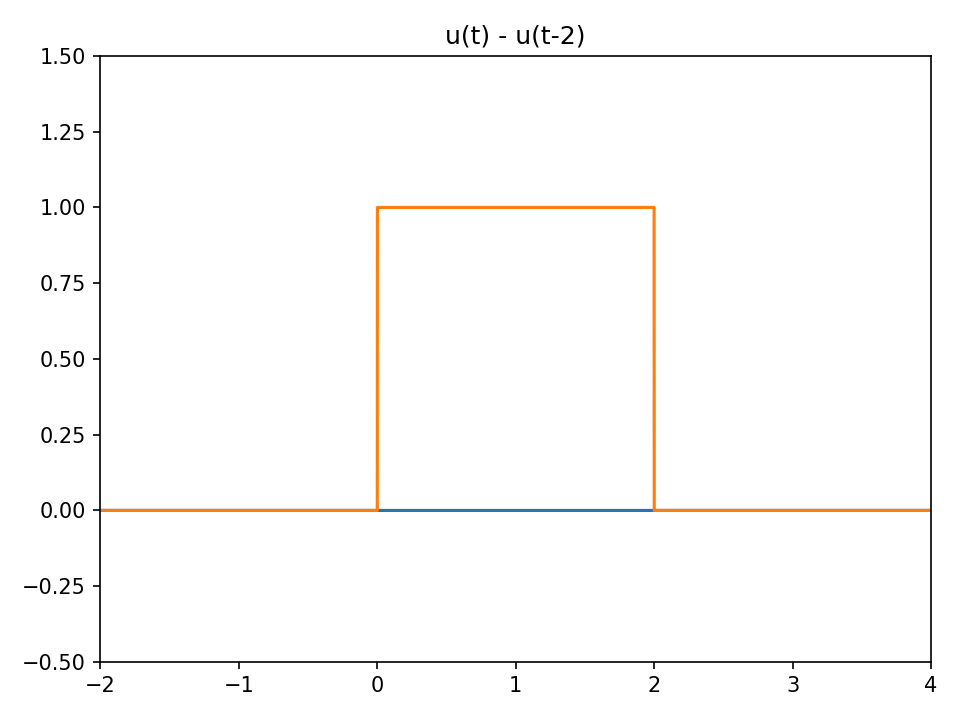
\includegraphics[height=3in]{./py-graphics/target/compesccont.png}
	\caption{Composición de dos escalones para formar una señal tipo pulso (tiempo continuo)}
	\label{fig:compesccont}
\end{figure}

\begin{figure}[htbp]
	\centering
	
\includegraphics[height=3in]{./graphics/compcontuno.eps}
	\caption{Composición de señales (tiempo continuo)}
	\label{fig:compcontuno}
\end{figure}

\begin{figure}[htbp]
	\centering
	
\includegraphics[height=3in]{./graphics/compescdisc.eps}
	\caption{Composición de dos escalones para formar un par de impulsos (tiempo discreto)}
	\label{fig:compescdisc}
\end{figure}

\begin{figure}[htbp]
	\centering
	
\includegraphics[height=3in]{./graphics/compcontdos.eps}
	\caption{Composición de señales (tiempo discreto)}
	\label{fig:compcontdos}
\end{figure}

\begin{figure}[htbp]
	\centering
	
\includegraphics[height=3in]{./graphics/comppreguno.eps}
	\caption{Pregunta sobre composición de señales (tiempo continuo)}
	\label{fig:comppreguno}
\end{figure}

\begin{figure}[htbp]
	\centering
	
\includegraphics[height=3in]{./graphics/comppregdos.eps}
	\caption{Pregunta sobre composición de señales (tiempo discreto)}
	\label{fig:comppregdos}
\end{figure}

\section{Señales de tiempo discreto}

\subsection{El impulso unitario}

Hemos visto que el impulso unitario de tiempo discreto se define como:
\begin{equation}
	\delta[n] =
	\begin{cases}
		0, & n \neq 0, \\ 
		1, & n = 0.
	\end{cases}
\end{equation}

Vea la Fig. (\ref{fig:impunidisc}).

\begin{figure}[htbp]
	\centering
	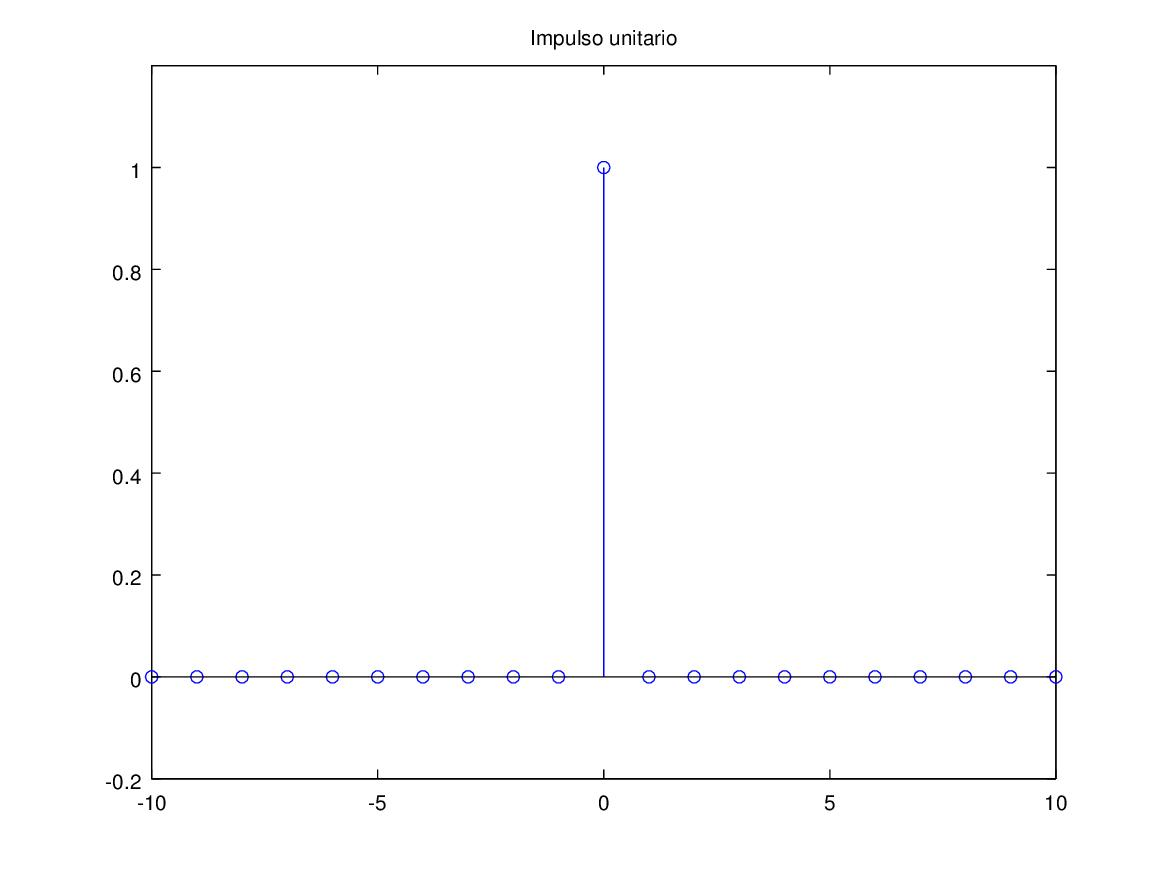
\includegraphics[height=2in]{./graphics/impunidisc.eps}
	\caption{Impulso unitario de tiempo discreto.}
	\label{fig:impunidisc}
\end{figure}

\subsection{El impulso unitario desplazado}

Desplazar un impulso unitario en el tiempo es sencillo. Veamos la
definición de $\delta[n-m]$ (La diferencia con la definición de
$\delta[n]$ aparece resaltada):
\begin{equation}
	\delta[n \mathbf{-m}] = 
	\begin{cases}
		1, & n \mathbf{-m} = 0, \\
		0, & n \mathbf{-m} \neq 0.
	\end{cases}
	\quad \longrightarrow \quad
	\delta[n \mathbf{-m}] = 
	\begin{cases}
		1, & n = \mathbf{m}, \\
		0, & n \neq \mathbf{m}.
	\end{cases}
\end{equation}

\subsection{El impulso multiplicado por un coeficiente}

La multiplicación de un impulso unitario $\delta[n]$ por un
coeficiente $a$ se define como:
\begin{equation}
	a \, \delta[n] = 
	\begin{cases}
		a, & n = 0, \\
		0, & n \neq 0.
	\end{cases}
\end{equation}

\subsection{La suma de dos impulsos desplazados en el tiempo y multiplicados por coeficientes}

La suma de dos impulsos desplazados en el tiempo y multiplicados por
coeficientes es una combinación lineal de impulsos. La podemos
definir de la siguiente forma:
\begin{equation}
	a_{1} \, \delta[n - m_{1}] + a_{2} \, \delta[n - m_{2}] = 
	\begin{cases}
		a_{1}, & n = m_{1}, \\
		a_{2}, & n = m_{2}, \\
		0, & (n \neq m_{1}) \wedge (n \neq m_{2}).
	\end{cases}
\end{equation}

\subsection{La suma de $N$ impulsos desplazados en el tiempo y multiplicados por coeficientes}

Podemos definir la suma de $N$ impulsos desplazados en el tiempo y multiplicados por
coeficientes $a_{k}$:
\begin{equation}
	x[n] = \sum_{k = 1}^{N} a_{k} \, \delta[n - k],
\end{equation}
donde para $m \in \mathbb{N}$:
\begin{equation}
	x[m] = \sum_{k = 1}^{N} a_{k} \, \delta[m - k] = a_{m},
\end{equation}
porque solo donde $m = k$ se cumple $\delta[m - k] = \delta[0] = 1$ y por lo tanto hay un solo impulso igual a $1$ que multiplica al coeficiente $a_{m}$. Todos los otros coeficientes están multiplicados por $0$.

\subsection{La señal como combinación lineal de impulsos}

\begin{enumerate}
	\item Consideremos una sucesión de impulsos $\delta[n - n_{0}]$ (ver Fig. \ref{fig:convone} y la Ec. \ref{claveuno}), multiplicados por los
	respectivos coeficientes $x[n_{0}]$:
	\begin{align}
		x[-2]\delta[n+2] &= 
		\begin{cases}
			x[-2], & n = -2, \\ 
			0, & n \neq -2.
		\end{cases} \\
		x[-1]\delta[n+1] &= 
		\begin{cases}
			x[-1], & n = -1, \\ 
			0, & n \neq -1.
		\end{cases} \\
		x[0]\delta[n] &= 
		\begin{cases}
			x[0], & n = 0, \\ 
			0, & n \neq 0.
		\end{cases} \\
		x[1]\delta[n-1] &= 
		\begin{cases}
			x[1], & n = 1, \\ 
			0, & n \neq 1.
		\end{cases} \\
		x[2]\delta[n-2] &= 
		\begin{cases}
			x[2], & n = 2, \\ 
			0, & n \neq 2.
		\end{cases}
	\end{align}
	y en general:
	\begin{equation}
		x[k]\delta[n-k] = 
		\begin{cases}
			x[k], & n = k, \\ 
			0, & n \neq k.
		\end{cases}
	\end{equation}
	
	\item Como podemos ver en la Fig. (\ref{fig:convone}), la suma de
	impulsos desplazados en el tiempo multiplicados por coeficientes
	adecuados equivalen a cualquier señal arbitraria $x[n]$.
	
	\begin{figure}[htbp]
		\centering
		\includegraphics[width=3in]{./graphics/convone.eps}
		\caption{Una señal como suma de impulsos desplazados en el
			tiempo multiplicados por coeficientes adecuados. Los impulsos
			desplazados $\delta[n-k]$ se representan $d[n-k]$. Sólo se
			muestran tres impulsos por razones de espacio.}
		\label{fig:convone}
	\end{figure}
	
	\item En efecto, agregando más impulsos desplazados y
	multiplicados adecuadamente podemos obtener una expresión que se
	puede escribir en forma general:
	\begin{equation}
		x[n] = \sum_{k=-\infty}^{\infty} x[k] \, \delta[n-k] .
		\label{cduna}
	\end{equation}
	
	\item La Ec. (\ref{cduna}) corresponde a la representación de una
	secuencia arbitraria $x[n]$ como:
	\begin{itemize}
		\item una combinación lineal de impulsos desplazados $\delta[n-k]$,
		\item donde los coeficientes de la combinación lineal son los valores $x[k]$.
	\end{itemize}
	
	\item Cada impulso desplazado $\delta[n-k]$ actúa
	como selector: suponga que elegimos un valor $n=n_{0}$ y entonces
	tenemos que:
	\begin{equation}
		x[n_{0}] = \sum_{k=-\infty}^{\infty} x[k] \, \delta[n_{0}-k] .
		\label{cddos}
	\end{equation}
	
	\item Recordemos la definición de impulso:
	\begin{equation}
		\delta[n] = 
		\begin{cases}
			1, & n = 0, \\ 
			0, & n \neq 0.
		\end{cases}
	\end{equation}
	El impulso ``vale'' $1$ cuando el índice $n$ (lo que aparece
	entre corchetes) vale $0$. Note que en la ec. (\ref{cddos}) sólo
	uno de los infinitos impulsos tiene un índice nulo,
	específicamente:
	\begin{equation}
		n_{0}-k=0.
	\end{equation}
	Entonces, de todos los infinitos términos sólo uno es no
	nulo ($k=n_{0})$. Así obtenemos la igualdad:
	\begin{equation}
		x[n_{0}] = x[n_{0}] .
	\end{equation}
	
	\item La utilidad de la ecuación (\ref{cduna}) es que expresa una secuencia
	\begin{equation}
		...x[-3], x[-2], x[-1], x[0], x[1], x[2], x[3]...
	\end{equation}
	como una sumatoria.
\end{enumerate}

\subsection{La señal multiplicada con un impulso}

\begin{enumerate}
	\item Consideremos una señal $x[n]$ a la que
	multiplicamos por un impulso $\delta[n - n_{0}]$. Hemos probado que:
	\begin{equation}
		x[n] \, \delta[n - n_{0}] = x[n_{0}] \, \delta[n - n_{0}].
	\end{equation}
	
	\item Recordemos que el impulso desplazado $\delta[n - n_{0}]$
	actúa como ``selector'' al multiplicar a una señal $x[n]$:
	la única muestra de $x[n]$ multiplicada por $1$ es $x[n_{0}]$,
	todas las demás se multiplican por $0$.
\end{enumerate}

\subsection{Escalado temporal}

\begin{enumerate}
	\item Supongamos que tenemos una señal $x[n]$ y la usamos para
	generar otra señal:
	\begin{equation}
		y[n] = x[3n].
		\label{escaladotemporaluno}
	\end{equation}
	¿Qué significa la Ec. (\ref{escaladotemporaluno})?
	Analicemos la siguiente tabla:
	
	\begin{center}
		\begin{tabular}{ccc}
			$n$ & $x[n]$ & $y[n] = x[3n]$ \\
			0   &  $x[0]$ & $x[0]$ \\
			1   &  $x[1]$ & $x[3]$ \\
			2   &  $x[2]$ & $x[6]$ \\
			3   &  $x[3]$ & $x[9]$ \\
			4   &  $x[4]$ & $x[12]$ \\
			5   &  $x[5]$ & $x[15]$ \\
			6   &  $x[6]$ & $x[18]$ \\
			... &  ... & ...
		\end{tabular}
	\end{center}
	
	\item Supongamos que tenemos una señal $x[n]$ y la usamos para
	generar otra señal:
	\begin{equation}
		y[n] = x\left[\frac{n}{3}\right].
		\label{escaladotemporaldos}
	\end{equation}
	¿Qué significa la Ec. (\ref{escaladotemporaldos})?
	Analicemos la siguiente tabla:
	
	\begin{center}
		\begin{tabular}{ccc}
			$n$ & $x[n]$  & $x[\frac{n}{3}]$ \\
			0   &  $x[0]$ & $x[0]$ \\
			1   &  $x[1]$ & $x[\frac{1}{3}]$ ?\\
			2   &  $x[2]$ & $x[\frac{2}{3}]$ ?\\
			3   &  $x[3]$ & $x[1]$ \\
			4   &  $x[4]$ & $x[\frac{4}{3}]$ ?\\
			5   &  $x[5]$ & $x[\frac{5}{3}]$ ?\\
			6   &  $x[6]$ & $x[2]$ \\
			7   &  $x[7]$ & $x[\frac{7}{3}]$ ?\\
			... &  ... & ...
		\end{tabular}
	\end{center}
	
	Como podemos ver, el problema es que el índice de una señal
	de tiempo discreto debe ser un número entero. Por lo tanto,
	deberíamos emplear la siguiente definición:
	\begin{equation}
		y[n] = 
		\begin{cases}
			x\left[\frac{n}{3}\right], & n = 3m, \\
			0, & n = 3m + 1, \\
			0, & n = 3m + 2.
		\end{cases}
	\end{equation}
	$\forall m \in \mathbb{N}$.
	
\end{enumerate}

\subsection{Tiempo inverso}

El caso de escalado temporal más sencillo es el del ``viaje al
pasado''. En este caso $y[n] = x[-n]$. Es algo como reproducir un audio "al revés".
Esta es una operación usada en dos casos. Existe un dispositivo denominado scrambler que se puede aplicar a un teléfono: divide el audio en segmentos y después los invierte en tiempo, segmento por segmento, antes de enviarlos por el canal de comunicación. En el otro lado del canal, un dispositivo similar recupera la señal original con el mismo proceso. La idea es que "nadie" pueda espiar la conversación, o mejor dicho que nadie la espíe fácilmente.

También hubo rumores que si se reproducen en tiempo inverso las canciones de rock se pueden oir mensajes ocultos. Un ejemplo con MATLAB:
\begin{verbatim}
	n = 1:5;
	x = randn(1, 5);
	subplot(2,1,1); stem(n, x); 
	subplot(2,1,2); stem(-n, x);
\end{verbatim}

\subsection{Desplazamiento en el tiempo}

\begin{enumerate}
	\item Supongamos una señal $x[n]$. Podemos desplazarla en el tiempo
	haciendo $y[n] = x[n - n_{0}]$.
	\item Por ejemplo, si $x_{1}[n] = \cos(2\pi \frac{2}{5} n)$,
	podemos obtener su versión desplazada cuatro muestras como
	$y_{1}[n] = x_{1}[n - 4] = \cos(2\pi \frac{2}{5} (n - 4))$.
\end{enumerate}

\subsection{Tren de impulsos}

\begin{enumerate}
	\item El impulso unitario está definido como:
	\begin{equation}
		\delta[n] = 
		\begin{cases}
			1, & n = 0, \\
			0, & n \neq 0.
		\end{cases}
	\end{equation}
	
	\item Podemos desplazar el impulso unitario definiendo:
	\begin{equation}
		\delta[n - n_{0}] = 
		\begin{cases}
			1, & n = n_{0}, \\
			0, & n \neq n_{0}.
		\end{cases}
	\end{equation}
	
	\item Por lo tanto, la siguiente definición:
	\begin{equation}
		\delta[n - k \, n_{0}] = 
		\begin{cases}
			1, & n = k \, n_{0}, \\
			0, & n \neq k \, n_{0}.
		\end{cases}
	\end{equation}
	donde $k$ es un número entero, nos da impulsos ubicados en múltiplos enteros de $n_{0}$.
	
	\item Si sumamos todos los impulsos obtenidos en el punto anterior,
	obtenemos el tren de impulsos:
	\begin{equation}
		x[n] = \sum_{k=-\infty}^{\infty} \delta[n - k \, n_{0}].
	\end{equation}
	
\end{enumerate}


\section{Señales de tiempo continuo}

\subsection{El pulso}

Un pulso unitario de tiempo continuo $p(t)$ de duración $\tau$ se define
como una diferencia de escalones unitarios con un factor $\frac{1}{\tau}$:
\begin{equation}
	p(t) = \frac{1}{\tau} \left(u(t) - u(t - \tau) \right),
\end{equation}
donde $\tau > 0$.

\subsection{El pulso desplazado}

Un pulso unitario de tiempo continuo $p(t)$ de duración $\tau$
desplazado en el tiempo $t_{0}$ se define como una diferencia de escalones
unitarios desplazados en el tiempo $t_{0}$:
\begin{equation}
	p(t-t_{0}) = \frac{1}{\tau} \left(u(t-t_{0}) - u(t - t_{0} - \tau) \right).
\end{equation}

\subsection{El impulso como límite del pulso}

Cuando $\tau$ tiende a $0$, el ancho del impulso tiende a $0$, su
altura tiende a $\infty$, y su área se mantiene igual a $1$.

\begin{figure}[htbp]
	\centering
	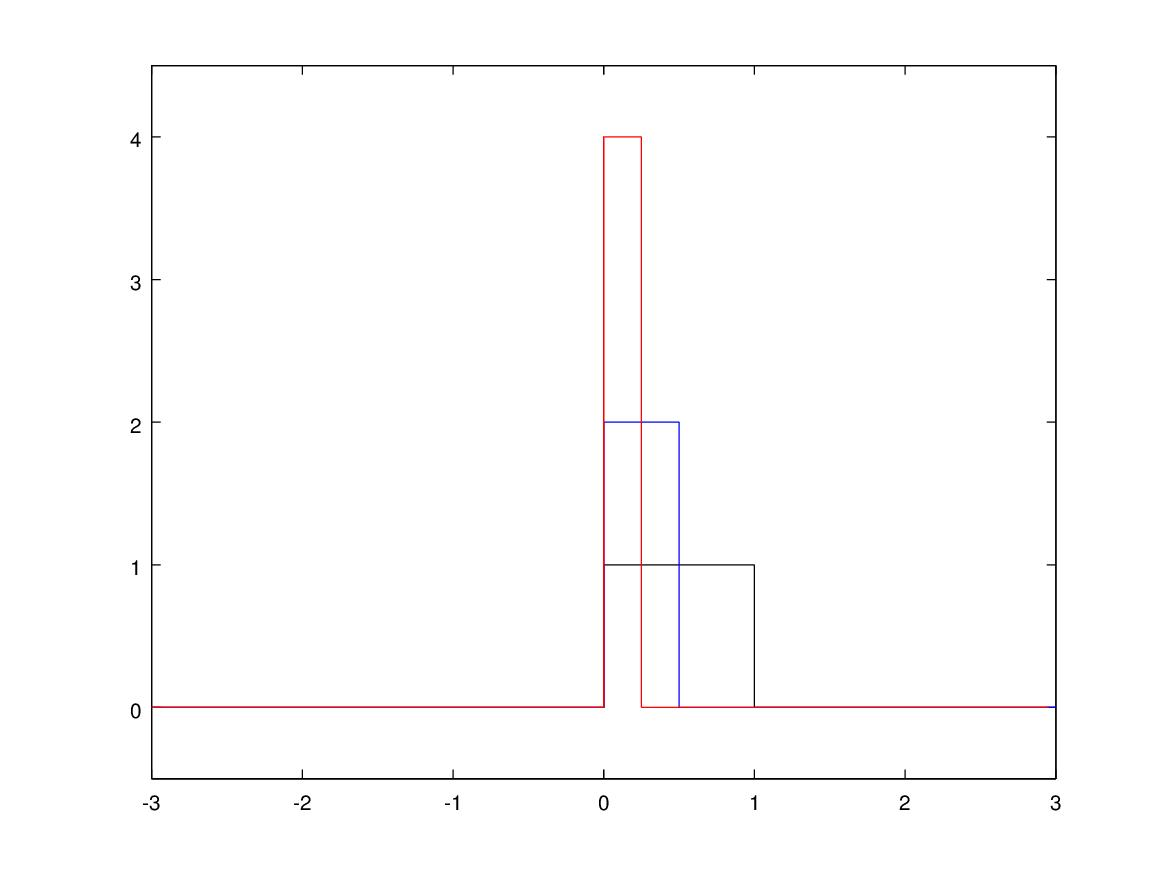
\includegraphics[width=3in]{./graphics/sucimpcont.eps}
	\caption{Impulso como límite de una sucesión de impulsos}
	\label{fig:sucimpcont}
\end{figure}

\begin{figure}[htbp]
	\centering
	\includegraphics[width=3in]{./graphics/lecture02_tex_gr7.eps}
	\caption{Otra función de área unitaria}
	\label{fig:lecture02texgr7}
\end{figure}

\begin{figure}[htbp]
	\centering
	\includegraphics[width=3in]{./graphics/lecture02_tex_gr8.eps}
	\caption{Otra función de área unitaria (y van tres)}
	\label{fig:lecture02texgr8}
\end{figure}

\subsection{La señal aproximada por una combinación lineal de pulsos}

\begin{figure}[htbp]
	\centering
	\includegraphics[width=3in]{./graphics/contconv222.eps}
	\caption{Señal aproximada por combinación lineal de pulsos}
	\label{fig:contconv222}
\end{figure}

La señal $x(t)$ puede aproximarse como una combinación lineal
de pulsos desplazados en el tiempo como puede verse en la figura
(\ref{fig:contconv222}), o analíticamente mediante los
siguientes pasos:
\begin{enumerate}
	\item Desplace los pulsos en el tiempo:
	\begin{align}
		\delta_{\Delta}(t+\Delta) &=
		\begin{cases}
			\frac{1}{\Delta}, & -\Delta \leq t < 0, \\ 
			0, & (t < -\Delta) \lor (0 \leq t).
		\end{cases} \\
		\delta_{\Delta}(t) &=
		\begin{cases}
			\frac{1}{\Delta}, & 0 \leq t < \Delta, \\ 
			0, & (t < 0) \lor (\Delta \leq t).
		\end{cases} \\
		\delta_{\Delta}(t-\Delta) &=
		\begin{cases}
			\frac{1}{\Delta}, & \Delta \leq t < 2\Delta, \\ 
			0, & (t < \Delta) \lor (2\Delta \leq t).
		\end{cases} \\
		&\vdots \nonumber \\
		\delta_{\Delta}(t-k\Delta) &=
		\begin{cases}
			\frac{1}{\Delta}, & k\Delta \leq t < (k+1)\Delta, \\ 
			0, & (t < k\Delta) \lor ((k+1)\Delta \leq t).
		\end{cases}
	\end{align}
	
	\item Multiplicando por $x(k\Delta)\Delta$ al $k$-ésimo pulso se obtiene:
	\begin{align}
		x(-\Delta)\delta_{\Delta}(t+\Delta)\Delta &=
		\begin{cases}
			\frac{x(-\Delta)}{\Delta}\Delta, & -\Delta \leq t < 0, \\ 
			0, & (t < -\Delta) \lor (0 \leq t).
		\end{cases} \\
		x(0)\delta_{\Delta}(t)\Delta &=
		\begin{cases}
			\frac{x(0)}{\Delta}\Delta, & 0 \leq t < \Delta, \\ 
			0, & (t < 0) \lor (\Delta \leq t).
		\end{cases} \\
		x(\Delta)\delta_{\Delta}(t-\Delta)\Delta &=
		\begin{cases}
			\frac{x(\Delta)}{\Delta}\Delta, & \Delta \leq t < 2\Delta, \\ 
			0, & (t < \Delta) \lor (2\Delta \leq t).
		\end{cases} \\
		&\vdots \nonumber \\
		x(k\Delta)\delta_{\Delta}(t-k\Delta)\Delta &=
		\begin{cases}
			\frac{x(k\Delta)}{\Delta}\Delta, & k\Delta \leq t < (k+1)\Delta, \\ 
			0, & (t < k\Delta) \lor ((k+1)\Delta \leq t).
		\end{cases}
	\end{align}
	
	\item Observe que un valor dado de $t$ (por ejemplo $t_{0}$) sólo puede pertenecer a \textbf{un} intervalo 
	$k\Delta \leq t < (k+1)\Delta$; por lo tanto, para $t_{0}$ solo uno de los productos puede ser distinto de $0$.
	Sumando los infinitos productos obtenemos:
	\begin{equation}
		x_{\Delta}(t) = \sum_{k=-\infty}^{\infty} x(k\Delta) \, \delta_{\Delta}(t-k\Delta) \, \Delta .
		\label{funcaspulsessum}
	\end{equation}
\end{enumerate}

\subsection{La señal como combinación lineal de impulsos}

Observe que en la ecuación (\ref{funcaspulsessum}) cuando 
$\Delta$ tiende a cero, $x_{\Delta}(t)$ tiende a $x(t)$.

\begin{equation}
	x(t) = \lim_{\Delta \to 0} x_{\Delta}(t) = \lim_{\Delta \to 0} \sum_{k=-\infty}^{\infty} x(k\Delta) \, \delta_{\Delta}(t-k\Delta) \, \Delta .
\end{equation}
Además, cuando $\Delta$ tiende a cero, la sumatoria se convierte en una integral:
\begin{equation}
	x(t) = \int_{-\infty}^{\infty} x(\tau) \, \delta(t-\tau) \, d\tau .
\end{equation}
Notemos que por la propiedad del muestreo, debe cumplirse:
\begin{equation}
	x(\tau) \, \delta(t-\tau) = x(t) \, \delta(t-\tau) ,
\end{equation}
y en ese caso:
\begin{equation}
	x(t) = x(t) \left( \int_{-\infty}^{\infty} \delta(t-\tau) \, d\tau \right),
\end{equation}
con lo que hemos probado que una función $x(t)$ puede escribirse
como una combinación lineal de impulsos.

\subsection{Desplazamiento en el tiempo}

\begin{enumerate}
	\item Supongamos una señal $x(t)$. Podemos desplazarla en el tiempo
	haciendo $y(t) = x(t - t_{0})$.
	\item Por ejemplo, si $x_{1}(t) = \cos(2\pi \frac{2}{10} t)$,
	podemos obtener su versión desplazada cuatro unidades de tiempo como
	$y_{1}(t) = x_{1}(t - 4) =  \cos(2\pi \frac{2}{10} (t - 4))$.
\end{enumerate}


\subsection{Escalado temporal}

\begin{enumerate}
	\item El escalado temporal es reemplazar la variable independiente $t$
	por otra variable a la que llamaremos $v$. La relación de estas
	variables está dada por una escala que simbolizaremos con la letra
	$a$. Por ejemplo, $t = a \, v$.
	
	\item Consideremos la señal $x(t) = \sin(2\pi t)$. Podemos
	realizar el escalado temporal $t = 2v$, para obtener $y(v) =
	\sin(4\pi v)$.
\end{enumerate}

\subsection{Tiempo inverso}

Un caso especial de escalado temporal es cuando la escala es
negativa. Por ejemplo, con $t = -v$, obtenemos el denominado tiempo inverso.

\subsection{Tren de impulsos}

\begin{enumerate}
	\item Supongamos una serie de impulsos desplazados en el tiempo $\delta(t)$,
	$\delta(t - T)$, $\delta(t - 2T)$, $\delta(t - 3T)$ y en
	general $\delta(t - kT)$, para $k$ entero.
	
	\item El par de impulsos sucesivos $\delta(t - kT)$ y $\delta(t - (k+1)T)$ está separado por un intervalo de tiempo $T$.
	
	\item El tren de impulsos es igual a la sumatoria de todos los
	impulsos $\delta(t - kT)$, para $k$ entero:
	\begin{equation}
		\Pi_{T}(t) = \sum_{k=-\infty}^{\infty} \delta(t - k \, T),
	\end{equation}
	donde los impulsos son no nulos en $t = kT$.
\end{enumerate}

\subsection{Muestreo}

El muestreo digital de una señal analógica (de tiempo continuo) nos permite obtener una señal de tiempo discreto. Si cumplimos ciertas condiciones, que vamos a estudiar durante este curso, 
es posible realizar un proceso inverso que nos permite recuperar la señal de tiempo continuo original.

El muestreo ideal es una función que toma los valores de $x(t)$ en los instantes $t = kT$, y $0$ para todo $t \neq kT$, 
donde $T$ es el período de muestreo y $k$ es una variable entera.

Matemáticamente, podemos representar la operación de muestreo como 
la multiplicación de una señal $x(t)$ con un tren de impulsos de período $T$:
\begin{equation}
	y(t) = x(t) \cdot \Pi_{T}(t) = x(t) \left( \sum_{k=-\infty}^{\infty} \delta(t - kT) \right).
\end{equation}
Entonces:
\begin{equation}
	y(t) = \sum_{k=-\infty}^{\infty} x(t) \, \delta(t - kT) = \sum_{k=-\infty}^{\infty} x(kT) \, \delta(t - kT).
\end{equation}


\section{Operaciones útiles, para tiempo discreto}

% Lathi, página 287

\subsection{Decimación}

Supongamos una señal $x[n]$. La decimación de una señal $x[n]$ es la generación de una nueva señal $y[n]$ mediante la eliminación de ciertas muestras de $x[n]$. Para eso multiplicamos $x[n]$ por:
\begin{equation}
	y[n] = x[n] \left( \sum_{k=-\infty}^{\infty} \delta[n - k \, N] \right).
\end{equation}
Si escribimos:
\begin{equation}
	y[n] = \sum_{k=-\infty}^{\infty} x[n] \, \delta[n - k \, N] =
	\sum_{k=-\infty}^{\infty} x[k \, N] \, \delta[n - k \, N],
\end{equation}
es evidente que para $n = qN + r$, con $q \in \mathbb{N}$ y $0 < r < N$, debe ser $y[n] = 0$.

\subsection{Interpolación}

Supongamos una señal $x[n]$. La interpolación de una señal $x[n]$ es la generación de una nueva señal $y[n]$ mediante la introducción de nuevas muestras 
calculadas, por ejemplo, como promedios de dos muestras consecutivas de $x[n]$. Por ejemplo:
\begin{align}
	y[0] &= x[0], \\
	y[1] &= (x[0] + x[1]) / 2, \\
	y[2] &= x[1], \\
	y[3] &= (x[1] + x[2]) / 2,
\end{align}
y así sucesivamente. Esta no es la única forma de interpolar. Es sólo un ejemplo de un tema que vamos a ver con más detenimiento cuando veamos transformada de Fourier.
	
	
	\chapter{Sistemas (y señales)}
	
	% Aquí puedes insertar la introducción al capítulo.
	
\section{Definiciones}

\begin{enumerate}
	\item Las señales son magnitudes naturales variables portadoras de información entre sistemas, representadas por funciones de variables independientes.
	\item Los sistemas son conjuntos de partes que interactúan entre si, con un propósito común.
	\item Los sistemas reciben señales de entrada para entregar señales de salida.
	\item Sistema de tiempo continuo es aquel que recibe, procesa y entrega solamente señales de tiempo continuo.
	\item Sistema de tiempo discreto es aquel que recibe, procesa y entrega solamente señales de tiempo discreto.
	\item Sistema híbrido es aquel que recibe, procesa y entrega señales de tiempo continuo y discreto.
	\item Los sistemas pueden representarse mediante relaciones entre las señales de entrada y salida.
	\item En el caso de sistemas de tiempo continuo, simbolizados
	\begin{equation}
		x(t) \rightarrow S \rightarrow y(t),
	\end{equation}
	podemos emplear los siguientes operadores matemáticos para describirlos:
	\begin{enumerate}
		\item Ecuaciones algebraicas
		\begin{equation}
			F(t, x(t), y(t)) = 0,
		\end{equation}
		donde $x(t)$ es la entrada e $y(t)$ es la salida del sistema. Por ejemplo:
		\begin{equation}
			y(t) - x(t) \, \cos(2 \, t) = 0.
		\end{equation}
		
		\item Ecuaciones diferenciales donde $x(t)$ es la entrada e $y(t)$ es la salida del sistema. Por ejemplo:
		\begin{equation}
			\frac{d y(t)}{dt} + 2 \, y(t) - x(t) = 0.
		\end{equation}
	\end{enumerate}
	
	\item En el caso de sistemas de tiempo discreto, simbolizados
	\begin{equation}
		x[n] \rightarrow S \rightarrow y[n],
	\end{equation}
	podemos emplear los siguientes operadores matemáticos para describirlos:
	\begin{enumerate}
		\item Ecuaciones algebraicas donde $x[n]$ es la entrada e $y[n]$ es la salida del sistema. Por ejemplo:
		\begin{equation}
			y[n] - x[n] \, 2^{-n} = 0.
		\end{equation}
		
		\item Ecuaciones de diferencias finitas donde $x[n]$ es la entrada e $y[n]$ es la salida del sistema. Por ejemplo:
		\begin{equation}
			y[n] - x[n] + x[n-1] - \frac{x[n-1]}{2} - y[n-1] - 2 \, y[n-2] + 4 \, y[n-3] = 0.
		\end{equation}
	\end{enumerate}
	
	\item Las descripciones de sistemas, ya sean ecuaciones algebraicas, ecuaciones diferenciales, o de diferencias son modelos matemáticos del sistema, y los podemos usar para análisis y diseño.
\end{enumerate}

\subsection{Ejemplos}

\subsubsection{Divisor resistivo de tensión}
Supongamos que tenemos un divisor resistivo de tensión donde la relación entre la tensión de entrada $v_{e}(t)$ y salida $v_{s}(t)$ es la ecuación:
\begin{equation}
	V_{s}(t) = \frac{R_{2}}{R_{1} + R_{2}} \, V_{e}(t). \label{divires}
\end{equation}
Esta es una ecuación algebraica de tiempo continuo. Ver Figura (\ref{circuitoeps}).

\subsubsection{Circuito RC Serie}
Supongamos que tenemos un circuito RC serie descripto por la ecuación diferencial:
\begin{equation}
	\frac{dv_{c}(t)}{dt} + \frac{1}{R \, C} \, v_{c}(t) = \frac{1}{R \, C} \, v_{s}(t). \label{rcserie}
\end{equation}
donde
\begin{itemize}
	\item $v_{c}(t)$ tensión en el capacitor,
	\item $v_{s}(t)$ tensión en la fuente,
	\item $R$ valor de la resistencia,
	\item $C$ valor del capacitor.
\end{itemize}
Ver Figura (\ref{circuitoeps}).

\subsubsection{Un negocio}
Supongamos que el dueño de un negocio repone todos los días la mercadería. La ecuación que describe la relación entre la cantidad de mercadería que entra en el depósito y el dinero necesario para comprarla es:
\begin{equation}
	t[n] = p \, (m - x[n]).
\end{equation}
donde
\begin{itemize}
	\item $x[n]$ es la cantidad de mercadería en el depósito,
	\item $m$ la cantidad máxima de mercadería que puede tener guardada,
	\item $p$ el precio unitario,
	\item $t[n]$ el pago por la compra del día $n$.
\end{itemize}
Esta es una ecuación algebraica de tiempo discreto.

\subsubsection{Cuenta bancaria}
Supongamos que tenemos una cuenta bancaria en la que obtenemos cierto interés mensual por mantener cierto depósito de dinero. La ecuación de diferencias que nos dice cuánto dinero tendremos el próximo mes es:
\begin{equation}
	y[n+1] = (1 + c/100) \, y[n] + x[n],
\end{equation}
donde
\begin{itemize}
	\item $y[n+1]$ dinero en la cuenta el próximo mes,
	\item $y[n]$ dinero en la cuenta este mes,
	\item $x[n]$ dinero depositado o extraído este mes,
	\item $c$ interés.
\end{itemize}
Esta es una ecuación de diferencias y por lo tanto, de tiempo discreto.

\subsubsection{Cálculo de raíces de polinomios}
Supongamos que tenemos que calcular \textbf{una} raíz del polinomio
\begin{equation}
	Q(x) = 0.
\end{equation}
Para obtener \textbf{una} solución podemos escribir la ecuación de diferencias
\begin{equation}
	x_{k+1} = x_{k} - \left(\frac{Q(x)}{\frac{d Q(x)}{dx}}\right)_{x=x_{k}}.
\end{equation}
Si damos a $x_{0}$ un valor suficientemente cercano a \textbf{la} raíz buscada del polinomio $Q(x)$, obtendremos una secuencia que converge rápidamente. Por ejemplo, si consideramos el polinomio
\begin{equation}
	Q(x) = x^{2} - 2 = 0, 
\end{equation}
calcularemos la raíz cuadrada de $2$. Por lo tanto, iteramos la ecuación de diferencias
\begin{equation}
	x_{k+1} = \frac{2 + x^{2}_{k}}{2 x_{k}}, \qquad x_{0} = 2,
\end{equation}
para obtener los primeros cinco valores de la secuencia
\begin{equation}
	\begin{array}{llllll}
		2 & 1.5 & 1.41667 & 1.41422 & 1.41421 & ...
	\end{array}
\end{equation}
que como vemos se acerca rápidamente al resultado correcto.

\section{Modelos}

Necesitamos describir los sistemas con los que trabajamos para poder analizarlos, verificar sus propiedades, o para diseñar nuevos sistemas. Como ya vimos, podemos usar ecuaciones diferenciales y ecuaciones de diferencias.

\subsection{Ecuaciones diferenciales}

Consideremos una ecuación diferencial
\begin{equation}
	\frac{d^{N} y(t)}{dt^{N}} + \sum_{i=0}^{N-1} a_{i} \, \frac{d^{i} y(t)}{dt^{i}} = \sum_{j=0}^{M} b_{j} \, \frac{d^{j} x(t)}{dt^{j}},
\end{equation}
donde $x(t)$ es la entrada, $y(t)$ es la salida, y los coeficientes $a_{i}$ y $b_{j}$ son constantes reales, $N \geq 1$, $M \geq 0$, $N > M$. Por ejemplo,
\begin{equation}
	\frac{d^{3}y(t)}{dt^{3}} + 3 \, \frac{d^{2}y(t)}{dt^{2}} + 2 \, \frac{dy(t)}{dt} + y(t) = x(t).
\end{equation}
Las ecuaciones diferenciales pueden escribirse como un sistema de ecuaciones diferenciales de primer orden denominadas ecuaciones de estado empleando variables de estado. Una posible definición de las variables de estado es la siguiente:
\begin{eqnarray}
	v_{1}   &=& y(t),                                               \\
	v_{k+1} &=& \frac{dv_{k}}{dt} = \frac{d^{k}y}{dt^{k}}, \quad 0 < k < N .
\end{eqnarray}
Con esta definición podemos escribir las ecuaciones de estado:
\begin{eqnarray}
	\frac{dv_{k}}{dt} &=& v_{k+1}, \quad 1 \leq k < N,  \\
	\frac{dv_{N}}{dt} &=& G(t, x(t), v_{1}, v_{2},...,v_{N}).
\end{eqnarray}
Por ejemplo, para
\begin{equation}
	\frac{d^{3}y(t)}{dt^{3}} + 3 \, \frac{d^{2}y(t)}{dt^{2}} + 2 \, \frac{dy(t)}{dt} + y(t) = x(t),
\end{equation}
definimos
\begin{equation}
	v_{1} = y(t),
\end{equation}
\begin{equation}
	\frac{dv_{1}}{dt} = v_{2} = \frac{dy(t)}{dt},
\end{equation}
\begin{equation}
	\frac{dv_{2}}{dt} = v_{3} = \frac{d^{2}y(t)}{dt^{2}},
\end{equation}
\begin{equation}
	\frac{dv_{3}}{dt} = \frac{d^{3}y(t)}{dt^{3}} = -v_{1} - 2 \, v_{2} - 3 \, v_{3} + x(t).
\end{equation}
En forma matricial:
\begin{equation}
	\begin{bmatrix}
		\dot{v}_{1} \\
		\dot{v}_{2} \\
		\dot{v}_{3}
	\end{bmatrix} 
	= \begin{bmatrix}
		0 & 1 & 0 \\
		0 & 0 & 1 \\
		-1 & -2 & -3
	\end{bmatrix} 
	\begin{bmatrix}
		v_{1}\\
		v_{2}\\
		v_{3}
	\end{bmatrix}
	+
	\begin{bmatrix}
		0 \\
		0 \\
		1
	\end{bmatrix} \, x(t).
\end{equation}
Las principales razones para emplear ecuaciones de estado son las siguientes:
\begin{enumerate}
	\item La teoría de ecuaciones diferenciales en esta notación permite trabajar con sistemas de varias entradas y varias salidas.
	\item Es muy sencillo programar computadoras para trabajar con esta notación.
	\item Esta notación permite realizar simulaciones por computadora de grandes sistemas con muchas entradas y muchas salidas.
\end{enumerate}

\subsection{Ecuaciones de diferencias}

Consideremos una ecuación de diferencias
\begin{equation}
	F(n, x[n], y[n-1],..., y[n-M+1]) = y[n].
\end{equation}
donde $x[n]$ es la entrada, $y[n]$ es la salida, y $M > 1$. Por ejemplo
\begin{equation}
	y[n+1] + \frac{1}{2} \, y[n] + \frac{1}{4} \, y[n-1] + \frac{1}{8} \, y[n-2] - x[n] = 0.
\end{equation}
Las ecuaciones de diferencias pueden escribirse como un sistema de ecuaciones de diferencias de primer orden denominadas ecuaciones de estado. Una posible definición de las variables de estado es:
\begin{eqnarray}
	v_{1}[n]   &=& y[n],                                               \\
	v_{k+1}[n] &=& v_{k}[n-1] = y[n-k], \quad 0 < k < M .
\end{eqnarray}
Con esta definición podemos escribir las ecuaciones de estado:
\begin{eqnarray}
	v_{k}[n+1] &=& v_{k+1}[n], \quad 1 \leq k < M,  \\
	v_{M}[n+1] &=& G(n, x[n], v_{1}[n], v_{2}[n],...,v_{M}[n]).
\end{eqnarray}
Por ejemplo, considerando la ecuación de diferencias
\begin{equation}
	y[n+1] + \frac{1}{2} \, y[n] + \frac{1}{4} \, y[n-1] + \frac{1}{8} \, y[n-2] - x[n] = 0,
\end{equation}
podemos definir las variables de estado
\begin{equation}
	v_{1}[n] = y[n-2],
\end{equation}
\begin{equation}
	v_{2}[n] = y[n-1] = v_{1}[n+1],
\end{equation}
\begin{equation}
	v_{3}[n] = y[n] = v_{2}[n+1],
\end{equation}
\begin{equation}
	v_{3}[n+1] = y[n+1] = - \frac{1}{2} \, v_{3}[n] - \frac{1}{4} \, v_{2}[n] - \frac{1}{8} \, v_{1}[n] + x[n].
\end{equation}
En forma matricial:
\begin{equation}
	\begin{bmatrix}
		v_{1}[n+1] \\
		v_{2}[n+1] \\
		v_{3}[n+1]
	\end{bmatrix} 
	= \begin{bmatrix}
		0 & 1 & 0 \\
		0 & 0 & 1 \\
		-\frac{1}{8} & -\frac{1}{4} & -\frac{1}{2}
	\end{bmatrix} 
	\begin{bmatrix}
		v_{1}[n]\\
		v_{2}[n]\\
		v_{3}[n]
	\end{bmatrix}
	+
	\begin{bmatrix}
		0 \\
		0 \\
		1
	\end{bmatrix} \, x[n].
\end{equation}

\subsection{De ecuación diferencial a ecuación de diferencias}

\subsubsection{Aproximando la derivada, hacia adelante}
Sabemos que por definición de derivada
\begin{equation}
	\frac{dy}{dt} = \lim_{\Delta \rightarrow 0} \frac{y(t+\Delta) - y(t)}{\Delta}.
\end{equation}
Entonces, si cambiamos el límite por un $\Delta$ pequeño, podemos escribir
\begin{equation}
	\frac{dy}{dt} \approx \frac{y[n+1] - y[n]}{\Delta}.
\end{equation}
Entonces, si tenemos la ecuación diferencial
\begin{equation}
	\frac{dy(t)}{dt} + 2 \, y(t) = x(t),
\end{equation}
resulta la ecuación de diferencias
\begin{equation}
	\frac{y[n+1] - y[n]}{\Delta} + 2 \, y[n] = x[n],
\end{equation}
o
\begin{equation}
	(y[n+1] - y[n]) + 2 \,  \Delta \, y[n] = \Delta \, x[n],
\end{equation}
y finalmente
\begin{equation}
	y[n+1] + (2 \, \Delta - 1) \, y[n] = \Delta \, x[n].
\end{equation}

\subsubsection{Aproximando la derivada, hacia atrás}
Podemos cambiar levemente la definición de derivada
\begin{equation}
	\frac{dy}{dt} = \lim_{\Delta \rightarrow 0} \frac{y(t) - y(t-\Delta)}{\Delta}.
\end{equation}
Entonces, si cambiamos el límite por un $\Delta$ pequeño, podemos escribir
\begin{equation}
	\frac{dy}{dt} \approx \frac{y[n] - y[n-1]}{\Delta}.
\end{equation}
Entonces, si tenemos la ecuación diferencial
\begin{equation}
	\frac{dy(t)}{dt} + 2 \, y(t) = x(t),
\end{equation}
resulta la ecuación de diferencias
\begin{equation}
	\frac{y[n] - y[n-1]}{\Delta} + 2 \, y[n] = x[n],
\end{equation}
o
\begin{equation}
	(y[n] - y[n-1]) + 2 \,  \Delta \, y[n] = \Delta \, x[n],
\end{equation}
y finalmente
\begin{equation}
	(1 + 2 \, \Delta) \, y[n] - y[n-1] = \Delta \, x[n].
\end{equation}

\subsubsection{Otra aproximación de derivada}
Otra forma de definir derivada es
\begin{equation}
	\frac{dy}{dt} = \lim_{\Delta \rightarrow 0} \frac{y(t+\Delta) - y(t-\Delta)}{2 \, \Delta}.
\end{equation}
Entonces podemos aproximar, para un $\Delta$ pequeño
\begin{equation}
	\frac{dy}{dt} \approx \frac{y(t+\Delta) - y(t-\Delta)}{2 \, \Delta}.
\end{equation}
Entonces, si tenemos la ecuación diferencial
\begin{equation}
	\frac{dy(t)}{dt} + 2 \, y(t) = x(t),
\end{equation}
resulta la ecuación de diferencias
\begin{equation}
	\frac{y[n+1] - y[n-1]}{2 \, \Delta} + 2 \, y[n] = x[n],
\end{equation}
o
\begin{equation}
	(y[n+1] - y[n-1]) + 4 \, \Delta \, y[n] = 2 \, \Delta \, x[n],
\end{equation}
y finalmente
\begin{equation}
	y[n+1] + 4 \, \Delta \, y[n] - y[n-1] = 2 \, \Delta \, x[n].
\end{equation}

\section{Diagrama de bloques}

\begin{enumerate}
	\item Es posible hacer descripciones de sistemas usando:
	\begin{enumerate}
		\item bloques que representan los distintos componentes del sistema.
		\item flechas que representan los flujos de señal entre los componentes (qué salida se conecta a qué entrada).
	\end{enumerate}
	
	\item Se pueden hacer diagramas de bloques del mismo sistema con énfasis en distintos aspectos:
	\begin{enumerate}
		\item Caja negra, con énfasis en los conjuntos de entradas y salidas.
		\item Caja blanca, con énfasis en las relaciones entre los distintos componentes del sistema.
	\end{enumerate}
	
\end{enumerate}

	\section{Interconexiones de sistemas}
	Existen varias formas de interconectar sistemas:
\begin{enumerate}
	\item Conexión serie.
	\item Conexión paralelo.
	\item Retroalimentación.
\end{enumerate}

	% Serie (cascada), paralelo y realimentación.

	\begin{figure}[htbp]
	\centering
	\begin{tikzpicture}[node distance=2.5cm, auto]
		
		\node (input) {};
		
		\node [block, right=of input] (sys1) {Sistema 1 \\ $S_1$};
		
		\node [block, right=of sys1] (sys2) {Sistema 2 \\ $S_2$};
		
		\node [right=of sys2] (output) {};
		
		% --- Conexiones ---
		\draw [signal] (input) -- node[label] {Entrada, $x(t)$} (sys1);
		\draw [signal] (sys1) -- node[label] {Señal Intermedia  \\ $w(t)$} (sys2);
		\draw [signal] (sys2) -- node[label] {Salida, $y(t)$} (output);
		
		% Dibujamos el rectángulo tomando como referencia la esquina superior izquierda de S1
		% y la esquina inferior derecha de S2, dándoles un margen (xshift/yshift).
		\draw[dashed, gray, thick, rounded corners=5pt]
		([xshift=-0.7cm, yshift=0.8cm]sys1.north west) rectangle 
		([xshift=0.7cm, yshift=-1.5cm]sys2.south east);
		
		% Colocamos el texto exactamente en el medio de ambos bloques, desplazado hacia abajo
		\path (sys1.south east) -- (sys2.south west) 
		node[midway, below=0.6cm, font=\small] {Sistema Total Comprendido};
		
	\end{tikzpicture}
	\caption{Ejemplo de interconexión de sistemas en cascada o serie. La salida del Sistema 1 es la entrada directa del Sistema 2.}
	\label{fig:interconexion_serie}
\end{figure}

\begin{figure}[htbp]
	\centering
	\begin{tikzpicture}[auto]
		
		% --- Definición de NODOS ---
		% Nodo de entrada invisible
		\node (input) at (0,0) {};
		
		% Punto de bifurcación (el punto negro donde la señal se divide)
		\node [branch] (split) at (2,0) {};
		
		% Sistemas en paralelo (arriba y abajo)
		\node [block] (sys1) at (4.5, 1.5) {Sistema 1 \\ $S_1$};
		\node [block] (sys2) at (4.5, -1.5) {Sistema 2 \\ $S_2$};
		
		% Sumador
		\node [sum] (adder) at (7, 0) {$+$};
		
		% Nodo de salida invisible
		\node (output) at (9.5, 0) {};
		
		% --- CONEXIONES ---
		% Entrada general al nodo de bifurcación
		\draw [signal] (input) -- node[label] {Entrada, $x(t)$} (split);
		
		% Bifurcación hacia los sistemas (el operador |- hace que la línea doble en ángulo recto)
		\draw [signal] (split) |- (sys1);
		\draw [signal] (split) |- (sys2);
		
		% Salidas de los sistemas hacia el sumador (el operador -| también hace el ángulo recto)
		% Se añade un pequeño "+" cerca del sumador para indicar que las señales se suman
		\draw [signal] (sys1) -| node[pos=0.25, label] {$y_1(t)$} (adder.north) 
		node[pos=0.9, right, font=\footnotesize] {$+$};
		
		\draw [signal] (sys2) -| node[pos=0.25, below=0.1cm, font=\small, align=center] {$y_2(t)$} (adder.south) 
		node[pos=0.9, right, font=\footnotesize] {$+$};
		
		% Salida general del sumador
		\draw [signal] (adder) -- node[label] {Salida, $y(t)$} (output);
		
		% --- CAJA PUNTEADA ---
		% Usamos coordenadas absolutas para asegurar que abarque todo (desde la bifurcación hasta el sumador)
		\draw[dashed, gray, thick, rounded corners=5pt]
		(1.5, 2.6) rectangle (7.6, -2.6);
		
		% Etiqueta inferior de la caja
		\node[font=\small] at (4.55, -2.3) {Sistema Total Comprendido};
		
	\end{tikzpicture}
	\caption{Ejemplo de interconexión de sistemas en paralelo. La señal de entrada se bifurca y excita a ambos sistemas simultáneamente, luego sus salidas se combinan en un sumador.}
	\label{fig:interconexion_paralelo}
\end{figure}
	
	\begin{figure}[htbp]
	\centering
	\begin{tikzpicture}[auto]
		
		% --- Definición de NODOS ---
		% Nodo de entrada invisible
		\node (input) at (0,0) {};
		
		% Sumador (donde se mezclan la entrada y la realimentación)
		\node [sum] (sum) at (2.5,0) {$+$};
		
		% Sistema 1 (Ruta de avance / Forward path)
		\node [block] (sys1) at (5,0) {Sistema 1 \\ $S_1$};
		
		% Punto de bifurcación para tomar la muestra de salida
		\node [branch] (branch) at (7.5,0) {};
		
		% Nodo de salida invisible
		\node (output) at (9.5,0) {};
		
		% Sistema 2 (Ruta de realimentación / Feedback path)
		% Lo colocamos debajo del Sistema 1
		\node [block] (sys2) at (5,-2) {Sistema 2 \\ $S_2$};
		
		% --- CONEXIONES ---
		% Entrada -> Sumador (Añadimos un pequeño "+" para indicar suma positiva)
		\draw [signal] (input) -- node[label] {Entrada, $x(t)$} 
		node[pos=0.85, above left, font=\footnotesize] {$+$} (sum);
		
		% Sumador -> Sistema 1 (Señal de error)
		\draw [signal] (sum) -- node[label] {$e(t)$} (sys1);
		
		% Sistema 1 -> Bifurcación -> Salida
		\draw [signal] (sys1) -- (branch) -- node[label] {Salida, $y(t)$} (output);
		
		% Bifurcación -> Sistema 2 (Baja y dobla a la izquierda)
		\draw [signal] (branch) |- (sys2);
		
		% Sistema 2 -> Sumador (Sigue a la izquierda y sube al sumador)
		% Añadimos un pequeño "-" para indicar realimentación negativa (típico en control)
		\draw [signal] (sys2) -| node[pos=0.9, right, font=\footnotesize] {$-$} (sum.south);
		
		% --- CAJA PUNTEADA ---
		% Coordenadas absolutas que envuelven todo el lazo (desde antes del sumador hasta la bifurcación)
		\draw[dashed, gray, thick, rounded corners=5pt]
		(1.5, 1.2) rectangle (8.2, -3.2);
		
		% Etiqueta inferior de la caja
		\node[font=\small] at (4.85, -2.9) {Sistema Total Comprendido};
		
	\end{tikzpicture}
	\caption{Ejemplo de interconexión de sistemas con realimentación (feedback). La salida del Sistema 1 se mide y se hace pasar por el Sistema 2, para luego restarse a la señal de entrada original.}
	\label{fig:interconexion_realimentacion}
\end{figure}

	\section{Propiedades Fundamentales}
	% Definiciones y métodos de verificación.
	
	\subsection{Sistemas sin memoria o estáticos}
	Los sistemas sin memoria o estáticos son aquellos en los que la salida actual depende únicamente de la entrada actual.
	\begin{equation}
		y(t) = 2 \, x(t),
	\end{equation}
	\begin{equation}
		y[n] = (x[n])^{3} + 4 \, x[n].
	\end{equation}
	
	\subsection{Sistemas con memoria o dinámicos}
	Los sistemas con memoria o dinámicos son aquellos en los que la salida actual depende de entradas de un momento distinto al actual. Por ejemplo:
	\begin{equation}
		\frac{dy(t)}{dt} + a \, y(t) = x(t),
	\end{equation}
	\begin{equation}
		\int_{0}^{t} x(\tau) \, d\tau = y(t),
	\end{equation}
	\begin{equation}
		y(t)=x(t)-x(t-\tau ),
	\end{equation}
	\begin{equation}
		y[n] = \sum_{k=0}^{2}x[n-k] = x[n] + x[n-1] + x[n-2].
	\end{equation}
		
\subsection{Sistemas inversos}
Un sistema $S$ tiene un sistema inverso $S^{-1}$ si su composición es tal que
\begin{equation}
	x(t) = S^{-1}(S(x(t))),
\end{equation}
\begin{equation}
	x[n] = S^{-1}(S(x[n])).
\end{equation}
Tengamos en cuenta que un sistema puede no tener sistema inverso. Por ejemplo:
\begin{equation}
	y(t) = (x(t))^{2}.
\end{equation}

\subsection{Sistemas causales}
Un sistema es causal o no anticipativo si su salida no depende de entradas futuras. Por ejemplo:
\begin{equation}
	y(t) = a \, x(t),
\end{equation}
\begin{equation}
	y[n] = x[n-1] + x[n-2].
\end{equation}
Todos los sistemas sin memoria son causales.

\subsection{Sistemas no causales}
Un sistema es no causal o anticipativo si su salida depende de entradas futuras. Por ejemplo, consideremos la ecuación:
\begin{equation}
	y[n] = \frac{1}{5} \, \sum_{k=-2}^{2}x[n-k].
\end{equation}
Calculemos la salida para $y[2]$. Expandiendo la sumatoria obtenemos:
\begin{equation}
	y[2] = \frac{1}{5} \, \left( x[2-(-2)] + x[2-(-1)] + x[2-0] + x[2-1] + x[2-2] \right).
\end{equation}
Simplificando, resulta:
\begin{equation}
	y[2] = \frac{1}{5} \left( x[4] + x[3] + x[2] + x[1] + x[0] \right).
\end{equation}
Como podemos ver, para calcular $y[2]$ necesitamos conocer las entradas futuras $x[4]$ y $x[3]$. Por lo tanto, el sistema es no causal.
	
\subsection{Sistemas dinámicos autónomos}
Un sistema dinámico es autónomo si:
\begin{itemize}
	\item Su ecuación diferencial es del tipo:
	\begin{equation}
		F\left(y(t), \frac{dy}{dt}, \dots, \frac{d^{M}y}{dt^{M}}\right) = 0,                  
	\end{equation}
	donde $y(t)$ es la salida del sistema.
	\item Su ecuación de diferencias es del tipo:
	\begin{equation}
		F(y[n], \dots, y[n-M]) = 0, 
	\end{equation}
	donde $y[n]$ es la salida del sistema.
\end{itemize}

\subsection{Sistemas dinámicos no autónomos}
Un sistema dinámico es no autónomo si:
\begin{itemize}
	\item Su ecuación diferencial es del tipo:
	\begin{equation}
		F\left(t, x(t), \frac{dx}{dt}, \dots, \frac{d^{N}x}{dt^{N}}, y(t), \frac{dy}{dt}, \dots, \frac{d^{M}y}{dt^{M}}\right) = 0,
	\end{equation}
	donde $x(t)$ es la entrada e $y(t)$ es la salida del sistema.
	\item Su ecuación de diferencias es del tipo:
	\begin{equation}
		F(n, x[n], \dots, x[n-N], y[n], \dots, y[n-M]) = 0, 
	\end{equation}
	donde $x[n]$ es la entrada e $y[n]$ es la salida del sistema.
\end{itemize}

\subsection{Linealidad homogénea}
Una función es lineal homogénea sí y solo sí:
\begin{equation}
	f(a \, x_{1} + b \, x_{2}) = a \, f(x_{1}) + b \, f(x_{2}).
\end{equation}
Por ejemplo, $y = f(x) = m \, x$ es una función lineal, porque se cumple:
\begin{equation}
	\begin{array}{ll}
		y_{1} & = m \, x_{1}, \\ 
		y_{2} & = m \, x_{2}, \\ 
		a \, y_{1}+ b \, y_{2} & = a \, m \, x_{1} + b \, m \, x_{2} = m \, (a \, x_{1}+ b \, x_{2}).
	\end{array}
\end{equation}
En cambio, $y = f(x) = m \, x + 1$ no es una función lineal como podemos verificar:
\begin{equation}
	\begin{array}{ll}
		y_{1} & = m \, x_{1}+1, \\ 
		y_{2} & = m \, x_{2}+1, \\ 
		a \, y_{1}+ b \, y_{2} & = m \, (a\, x_{1}+ b \, x_{2}) + (a+b) \neq m \, (a \, x_{1}+b \, x_{2}) + 1.
	\end{array}
\end{equation}

\subsection{Sistemas lineales}
Se dice que un sistema $S$ es lineal si su respuesta para una entrada compuesta $a \, x_{1}+b \, x_{2}$ cumple con la siguiente propiedad:
\begin{equation}
	S(a \, x_{1}+ b\, x_{2}) = a \, S(x_{1}) + b \, S(x_{2}),
\end{equation}
conocida como principio de superposición.

\subsection{Sistemas no lineales}
Se dice que un sistema $f$ es no lineal si su respuesta para una entrada compuesta $a \, x_{1}+b \, x_{2}$ cumple con la siguiente propiedad:
\begin{equation}
	f(a \, x_{1}+b \, x_{2}) \neq a \, f(x_{1}) + b \, f(x_{2}),
\end{equation}
y por lo tanto, \textbf{NO} cumple con el principio de superposición. Por ejemplo, esta ecuación diferencial no es lineal:
\begin{equation}
	\frac{dy(t)}{dt} = y(t) \, (M - y(t)) + x(t).
\end{equation}

\subsection{Puntos de equilibrio}
\begin{enumerate}
	\item Un sistema dinámico de tiempo continuo con ecuación de estado $\mathbf{\dot x} = f(\mathbf{x})$, tiene un punto de equilibrio $\mathbf{x_{e}}$ si se satisface la siguiente ecuación:
	\begin{equation}
		\mathbf{0} = f(\mathbf{x_{e}}).
	\end{equation}
	
	\item Un sistema dinámico de tiempo discreto con ecuación de estados $\mathbf{x_{k+1}} = f(\mathbf{x_{k}})$, tiene un punto de equilibrio $\mathbf{x_{e}}$ si se satisface la siguiente ecuación:
	\begin{equation}
		\mathbf{x_{e}} = f(\mathbf{x_{e}}).
	\end{equation}
\end{enumerate}

\subsection{Sistemas dinámicos estables}
\begin{enumerate}
	\item \textbf{Sistemas no autónomos} (BIBO: Bounded Input Bounded Output) La salida permanece acotada para entradas acotadas.
	\item \textbf{Sistemas autónomos} El sistema estable evoluciona por si sólo a un estado de equilibrio.
\end{enumerate}
	
\subsection{Sistemas invariantes en el tiempo}
Un sistema invariante en el tiempo es aquél cuyas características y comportamiento están fijas en el tiempo. Este tipo de sistemas para una entrada determinada generan la misma salida independientemente del momento de aplicación.
\begin{enumerate}
	\item La salida $y(t)$ para la entrada $x(t+t_{0})$ es independiente del valor $t_{0}$.
	\item La salida $y[n]$ para la entrada $x[n + n_{0}]$ es independiente del valor $n_{0}$.
\end{enumerate}

\subsection{Sistemas variantes en el tiempo}
Si un sistema no es invariante en el tiempo, entonces se dice que es variante. En realidad, todos los sistemas físicos \textbf{son} variantes, debido al deterioro natural impuesto por la termodinámica. Lo que sucede es que con una escala de tiempo adecuada, el deterioro puede ignorarse.

\subsection{Ejemplos}

\subsubsection{Primer caso}
Supongamos un sistema definido por:
\begin{equation}
	y(t) = g(t) \, x(t).
\end{equation}
¿Es lineal? Si, como podemos ver en las siguientes ecuaciones:
\begin{eqnarray}
	y(t) &=& g(t) \, (a \, x_{1}(t) + b \, x_{2}(t)) = a \, g(t) \, x_{1}(t) + b \, g(t) \, x_{2}(t),    \\
	y(t) &=& a \, y_{1}(t) + b \, y_{2}(t).
\end{eqnarray}
¿Es invariante en el tiempo? No, como podemos ver:
\begin{eqnarray}
	y_{1}(t) &=& g(t) \, x_{1}(t) \rightarrow y_{1}(t-\tau) = g(t-\tau) \, x_{1}(t-\tau), \\
	y_{2}(t) &=& g(t) \, x_{1}(t-\tau).
\end{eqnarray}
¿Tiene memoria? No, porque no necesitamos conocer otro valor que el de la entrada actual para calcular la salida.

\subsubsection{Segundo caso, tiempo continuo}
El sistema:
\begin{equation}
	y(t) = S(x(t)) = 2 x(t),
\end{equation}
es un sistema sin memoria o estático de tiempo continuo que tiene un sistema inverso:
\begin{equation}
	S^{-1}(x(t)) = \frac{1}{2} x(t).
\end{equation}

\subsubsection{Tercer caso, tiempo discreto}
El sistema:
\begin{equation}
	y[n] = \sum_{k=0}^{\infty} x[n-k],
\end{equation}
es un sistema con memoria o dinámico de tiempo discreto que tiene un sistema inverso:
\begin{eqnarray}
	x[n] &=& y[n] - y[n-1] = \left(\sum_{k=0}^{\infty} x[n-k]\right) - \left( \sum_{k=0}^{\infty}x[n-1-k]\right), \\
	x[n] &=& x[n] + \left( \sum_{k=1}^{\infty} x[n-k]\right) - \left(\sum_{k=0}^{\infty}x[n-1-k]\right).
\end{eqnarray}
Haciendo el cambio de variable $p = k - 1$ en la primera sumatoria, obtenemos:
\begin{equation}
	x[n] = x[n] + \left( \sum_{p=0}^{\infty} x[n-1-p]\right) - \left(\sum_{k=0}^{\infty} x[n-1-k]\right).
\end{equation}
	
\chapter{Software clásico}

\section{Introducción a Matlab / Octave}

Matlab y Octave son intérpretes que nos permiten realizar cálculos numéricos, incluso con números complejos, vectores y matrices, y realizar gráficos en distintas representaciones.

En este apunte, mostramos algunas de las operaciones y comandos básicos para la operación interactiva. 

\subsection{La línea de comandos}

\begin{enumerate}
	
	\item Cuando Matlab/Octave comienza a ejecutarse, aparece una ventana tipo consola (sin interfaz gráfica), y una línea marcada con el símbolo \verb->>-. Esta es la línea de comandos, donde escribimos las diferentes órdenes.
	
	\item Para probar podemos escribir:
	\begin{verbatim}
		2 + 2
		3 - 5
		3 / 1.4
		2 * pi / 4
		(1 + 2 * i) / (1 - 2 * i)
	\end{verbatim}
	Nota: $i$ es la unidad imaginaria.
	
	\item En las últimas versiones de Matlab/Octave, a medida que vamos escribiendo comandos, estos quedan registrados en un historial de comandos, que podemos revisar más tarde y recordar lo hecho.
	
	\item El comando \texttt{diary} nos permite grabar en un archivo de texto todas las órdenes, datos y resultados de una sesión. Para usar el comando \texttt{diary} escribamos en la línea de comandos:
	\begin{verbatim}
		>> diary 'archivo.txt'
	\end{verbatim}
	
	\item La idea de esta clase es generar un archivo, denominado \verb-archivo.txt-, con todas las órdenes dadas.
\end{enumerate}

\subsection{El sistema de ayuda}

\begin{enumerate}
	\item Para ver cómo se usa un comando es posible escribir en la línea de comandos:
	\begin{verbatim}
		>> help comando
	\end{verbatim}
	donde \texttt{comando} es el nombre del comando que nos interesa.
	
	\item La orden \texttt{help comando} nos da una descripción del comando y posiblemente una lista de comandos relacionados.
	\begin{verbatim}
		>> help diary
	\end{verbatim}
\end{enumerate}

\subsection{Valores escalares}

\begin{enumerate}
	\item Como hemos visto, operamos con números reales y complejos, también llamados escalares.
	\item La unidad imaginaria puede escribirse como $i$ o $j$.
	\item Probemos los siguientes comandos:
	\begin{verbatim}
		(1 + 2 * j) * (1 - 2 * i)
		45 * (56 + i) - 34 * (16 - 32 * j)
	\end{verbatim}
\end{enumerate}

\subsection{Valores matriciales o arreglos}

\begin{enumerate}
	\item Matlab/Octave trabaja también con arreglos de reales y complejos.
	\item Podemos crear un vector fila escribiendo:
	\begin{verbatim}
		[ 1 + 2 * i  1 - 3 * i ]
	\end{verbatim}
	o separando con comas:
	\begin{verbatim}
		[ 1 + 2 * i, 1 - 3 * i ]
	\end{verbatim}
	
	\item Podemos crear un vector columna escribiendo:
	\begin{verbatim}
		[ 1 + 2 * i; 1 - 3 * i ]
	\end{verbatim}
	o separando con un salto de línea:
	\begin{verbatim}
		[ 1 + 2 * i
		1 - 3 * i ]
	\end{verbatim}
\end{enumerate}

\subsection{Metáfora de Matlab / Octave}

Podemos suponer, a modo de metáfora, que disponemos de un pizarrón donde escribimos las cuentas que vamos haciendo, línea por línea.

\subsection{Variables}

\begin{enumerate}
	
	\item A diferencia de una calculadora, Matlab/Octave permite asignar nombres a los diferentes valores. Esta combinación de nombre y valor recibe el nombre de variable.
	
	\item A continuación vemos ejemplos de los distintos tipos de variables. La constante $i$ es la unidad imaginaria, y ya está definida por defecto. El símbolo \texttt{\%} se usa para indicar que aquello escrito a su derecha hasta el fin de la línea es un comentario y no será ejecutado por el intérprete.
	
	\item Pruebe ingresar lo que aparece después de \verb->>-:
	\begin{verbatim}
		>> a = 5            % escalar real
		>> b = 5 + 10 * i   % escalar complejo
		>> c = [1 2 3]      % vector fila
		>> d = [1, 2, 3]    % otra forma de escribir un vector fila
		>> e = [1; 2; 3]    % un vector columna
		>> f = [1, 2, 3; 4, 5, 6; 7, 8, 9] % una matriz 3 x 3
	\end{verbatim}
\end{enumerate}

\subsection{Continuando con la metáfora de Matlab / Octave}

\begin{enumerate}
	\item Las variables son similares a divisiones que dibujamos en nuestro pizarrón, en las cuales escribimos los valores y los nombres respectivos.
	\item El espacio ocupado por las variables en memoria se denomina espacio de trabajo (workspace).
\end{enumerate}

\subsubsection{Los comandos who y what}

\begin{enumerate}
	\item El comando \texttt{who} da una lista de las variables presentes en el espacio de trabajo actual.
	\item Pruebe ingresar:
	\begin{verbatim}
		>> help who
	\end{verbatim}
	
	\item El comando \texttt{what} da una lista de archivos de código presentes en el directorio de trabajo actual. También puede probar \texttt{ls} o \texttt{dir} para listar todos los archivos. Verifique cuál es el directorio por defecto.
	\item Pruebe ingresar:
	\begin{verbatim}
		>> help what
	\end{verbatim}
	
	\item Ejecute:
	\begin{verbatim}
		>> who
		>> what
	\end{verbatim}
\end{enumerate}

\subsection{Operaciones con números complejos}

\begin{enumerate}
	\item A continuación vemos algunas de las operaciones que pueden realizarse con números complejos. Pruebe ingresar:
	\begin{verbatim}
		>> x = 3 + 4 * i
		>> real(x)  % 3
		>> imag(x)  % 4
		>> conj(x)  % 3 - 4 * i
		>> abs(x)   % 5
		>> angle(x) % 0.9273 (en radianes)
	\end{verbatim}
\end{enumerate}

\subsection{Raíces y coeficientes de un polinomio}

\begin{enumerate}
	\item Supongamos que tenemos un polinomio general:
	\begin{equation}
		b_{n}x^{n}+b_{n-1}x^{n-1}+...+b_{0}=0.
	\end{equation}
	Para hallar las raíces del polinomio podemos colocar sus coeficientes en un vector ordenado (de mayor a menor grado) y usar la función \texttt{roots}:
	\begin{verbatim}
		p = [bn, ..., b0];
		roots(p)
	\end{verbatim}
	
	\item Supongamos que tenemos que hallar las raíces del polinomio $x^{2}+2x+3=0$. Escribamos entonces:
	\begin{verbatim}
		p = [1, 2, 3];
		roots(p)
	\end{verbatim}
	
	\item Supongamos ahora que conocemos las raíces y necesitamos hallar los coeficientes del polinomio originario. Podemos usar la función \texttt{poly}:
	\begin{verbatim}
		>> r = [-1.0, 2.7, -3.1, -3.1];
		>> poly(r)
	\end{verbatim}
	
	\item Por ejemplo, si las raíces son $1, -1+2i, -1-2i$, entonces:
	\begin{verbatim}
		>> r = [1, -1+2*i, -1-2*i];
		>> poly(r)
	\end{verbatim}
	
	\item Pruebe con el vector correspondiente al polinomio $x^4+2x^3+3x^2+4x+5$:
	\begin{verbatim}
		>> p = [1, 2, 3, 4, 5]; 
		>> r = roots(p)
		>> poly(r)
	\end{verbatim}
	
	\item ¿Cuál le parece que es el resultado de la siguiente orden?
	\begin{verbatim}
		poly(roots(p))
	\end{verbatim}
	
	\item Pruebe las siguientes órdenes para mayor información:
	\begin{verbatim}
		>> help roots
		>> help poly
	\end{verbatim}
\end{enumerate}

\subsection{Generación de vectores y matrices}

\begin{enumerate}
	\item Matlab permite la generación de secuencias de valores y su asignación a vectores mediante un mecanismo sumamente eficiente basado en el operador dos puntos (\texttt{:}).
	\item Por ejemplo, supongamos que deseamos obtener un vector fila con una lista de números que comienza en $1$, termina en $2$ con incrementos de $0.1$. Escribiendo:
	\begin{verbatim}
		>> t = 1:0.1:2
	\end{verbatim}
	se obtiene el vector deseado. Observe que $t$ está formado por una fila de once columnas ($1 \times 11$).
	
	\item Si deseamos generar $t$ como un vector columna, podemos transponerlo agregando un apóstrofe (\texttt{'}):
	\begin{verbatim}
		>> t = (1:0.1:2)'
	\end{verbatim}
	
	\item Practique los siguientes puntos:
	\begin{enumerate}
		\item Genere un vector que contenga valores entre $-2$ y $2$ espaciados cada $0.01$.
		\item Para generar matrices llenas de ceros o unos podemos usar las funciones \texttt{zeros} y \texttt{ones}, respectivamente. Encuentre cómo se usan estas funciones con la ayuda (\texttt{help}) y haga un ejemplo con cada una.
	\end{enumerate}
\end{enumerate}

\subsection{Operaciones sobre vectores y matrices, primera parte}

\begin{enumerate}
	\item Matlab permite realizar operaciones con matrices siempre que sus dimensiones sean compatibles. Primero veremos cuál es la función que nos permite averiguar las dimensiones de una variable.
	\item Pruebe los siguientes comandos:
	\begin{verbatim}
		>> t = 1:0.1:2;
		>> size(t)
		>> size(t')
	\end{verbatim}
	
	\item Las operaciones algebraicas de suma, resta y multiplicación por escalares son muy simples. Pruebe:
	\begin{verbatim}
		>> t + 2
		>> t - 2
		>> t * 2
	\end{verbatim}
	
	\item Estas operaciones se realizan sumando, restando o multiplicando cada elemento individual del vector por el escalar. De la misma forma se aplican funciones trigonométricas elemento a elemento:
	\begin{verbatim}
		>> cos(t)
		>> sin(2 * t - 1)
	\end{verbatim}
	
	\item Supongamos ahora que queremos elevar al cuadrado cada elemento de un vector. Pruebe con los comandos:
	\begin{verbatim}
		>> t .* t
		>> t .^ 2
	\end{verbatim}
	
	\item Para realizar el producto matricial interno y externo de dos vectores escriba:
	\begin{verbatim}
		>> t' * t
		>> t * t'
	\end{verbatim}
	Indique la diferencia estructural entre los resultados de ambas operaciones.
\end{enumerate}

\subsection{Operaciones sobre vectores y matrices, segunda parte}

Es posible realizar operaciones vectoriales forzando el cálculo "elemento a elemento" (point-wise) agregando un punto (\texttt{.}) antes del operador matemático.
\begin{enumerate}
	\item Definamos:
	\begin{verbatim}
		x = [-1 2]
		y = [3 4]
	\end{verbatim}
	
	\item Si calculamos \texttt{z = x + y} resulta \texttt{z = [(-1 + 3) , (2 + 4)]} = \texttt{[2, 6]}.
	\item Si calculamos \texttt{z = x * y} obtendremos un mensaje de error de álgebra lineal, diciendo que las matrices no tienen dimensiones internas compatibles para ser multiplicadas.
	\item ¿Cómo podemos obtener el producto elemento a elemento $[-1 \cdot 3, 2 \cdot 4]$? Empleando el operador \texttt{.*}:
	\begin{verbatim}
		x .* y
	\end{verbatim}
	y obtendrá:
	\begin{verbatim}
		[-3 8]
	\end{verbatim}
	
	\item Lo mismo se debe hacer con la división:
	\begin{verbatim}
		x ./ y
	\end{verbatim}
	y la exponenciación:
	\begin{verbatim}
		x .^ y
	\end{verbatim}
	o
	\begin{verbatim}
		x .^ 2
	\end{verbatim}
\end{enumerate}

\subsection{Operaciones sobre vectores y matrices, tercera parte}

\begin{enumerate}
	
	\item Ingresemos un vector:
	\begin{verbatim}
		v = [1, 2, 3, 4, 5, 6, 7]
	\end{verbatim}
	
	\item Podemos acceder a los valores almacenados empleando la notación \verb-v(i)-, donde $i$ es un número entero (índice) mayor o igual a $1$. Pruebe:
	\begin{verbatim}
		v(1)
	\end{verbatim}
	
	\item También podemos extraer una porción (slice) del vector $v$ escribiendo \verb-v(i:j)-, donde $i \leq j$. Pruebe:
	\begin{verbatim}
		v(2:7)
		v(1:6)
		v(2:7) - v(1:6)  % Útil para calcular diferencias finitas
	\end{verbatim}
	
	\item Observe que la palabra reservada \texttt{end} permite acceder al último elemento dinámicamente:
	\begin{verbatim}
		v(2:end) - v(1:end-1)
	\end{verbatim}
	
	\item Matlab/Octave tiene una extensa librería de funciones de álgebra lineal aplicables a matrices. A continuación mostramos una pequeña tabla representativa:
	\begin{center}
		\begin{tabular}{ll}
			\textbf{Comando} & \textbf{Resultado} \\ \hline
			\texttt{det} & Determinante de una matriz cuadrada \\
			\texttt{eig} & Autovalores y autovectores \\
			\texttt{inv} & Inversa matricial \\
			\texttt{svd} & Descomposición en valores singulares (SVD) \\
			\texttt{cond} & Número de condición de una matriz \\
		\end{tabular}
	\end{center}
	
	\item Supongamos un sistema de 2 ecuaciones lineales con dos incógnitas representable matricialmente como $Ax=b$, donde:
	\begin{verbatim}
		A = [1, 2; 2, 1];
		b = [1; 2];
	\end{verbatim}
	
	\begin{enumerate}
		\item Matemáticamente, este sistema se resuelve calculando $x = A^{-1}b$. En código podríamos escribir:
		\begin{verbatim}
			x = inv(A) * b;
		\end{verbatim}
		\textbf{Nota importante:} Aunque usar \texttt{inv()} es correcto teóricamente, numéricamente es ineficiente y propenso a errores de precisión en matrices grandes. El método recomendado y optimizado en Matlab/Octave es usar el operador de "división izquierda" (\texttt{\textbackslash}):
		\begin{verbatim}
			x = A \ b;
		\end{verbatim}
		
		\item ¿Cómo puede verificar que el resultado es correcto? Calculando el vector de error (residuo):
		\begin{verbatim}
			e = A * x - b;
			e' * e   % Suma de los errores al cuadrado (debe ser muy cercana a 0)
		\end{verbatim}
		
		\item Resuelva los siguientes sistemas de ecuaciones y calcule los errores correspondientes:
		\begin{eqnarray}
			A_{1} = \begin{bmatrix} 1 & 1 \\ -1 & 1 \end{bmatrix}, & b_{1} = \begin{bmatrix} 0 \\ 1 \end{bmatrix}, \\
			A_{2} = \begin{bmatrix} 100.0 & 100.0 \\ 100.0 & 100.0 + 5 \cdot eps \end{bmatrix}, & b_{2} = \begin{bmatrix} 0 \\ 1 \end{bmatrix}.
		\end{eqnarray}
		
		\item ¿Para qué sirve la constante integrada \texttt{eps}? (Pista: es la distancia desde $1.0$ hasta el próximo número de punto flotante más grande en precisión doble).
		
		\item Busque en la ayuda el listado completo de operaciones matriciales (\texttt{help matfun}).
	\end{enumerate}
\end{enumerate}

\subsection{Graficación de funciones 2D}

\begin{enumerate}
	\item Para graficar funciones existen distintos comandos. Escriba:
	\begin{verbatim}
		>> t = 0:0.1:2*pi;
		>> y = cos(2 * t - 1);
		>> figure(1); plot(t, y);
		>> figure(2); stem(t, y);
	\end{verbatim}
	
	\item El comando \texttt{figure} crea o selecciona ventanas gráficas independientes. \texttt{plot} dibuja una señal de tiempo continuo uniendo los puntos con líneas, mientras que \texttt{stem} grafica la secuencia de valores discretos explícitos (ideal para señales muestreadas).
	
	\item Estos comandos admiten un tercer parámetro opcional para configurar el estilo (\verb-plot(t, y, 'formato')-). El formato es una cadena de texto (ej: \texttt{'r*: '}) que combina:
	\begin{itemize}
		\item \textbf{Colores:} \texttt{y} (amarillo), \texttt{m} (magenta), \texttt{c} (cyan), \texttt{r} (rojo), \texttt{g} (verde), \texttt{b} (azul), \texttt{w} (blanco), \texttt{k} (negro).
		\item \textbf{Marcadores:} \texttt{.} (punto), \texttt{o} (círculo), \texttt{x} (equis), \texttt{*} (asterisco), \texttt{s} (cuadrado).
		\item \textbf{Líneas:} \texttt{-} (sólida), \texttt{:} (punteada), \texttt{-.} (raya y punto), \texttt{--} (discontinua).
	\end{itemize}
	
	\item Por ejemplo:
	\begin{verbatim}
		>> plot(t, y, 'c+:')
	\end{verbatim}
	dibuja una línea punteada celeste uniendo las cruces ubicadas en cada dato.
	
	\item Observe los comandos complementarios para enriquecer el gráfico:
	\begin{verbatim}
		>> t = 0:0.1:2*pi;
		>> clf; plot(t, cos(t), 'm:o');
		>> grid on;
		>> xlabel('Tiempo (s)');
		>> ylabel('Amplitud (V)');
		>> title('Función periódica');
	\end{verbatim}
	
	\item El comando \texttt{subplot} permite colocar múltiples gráficos en la misma ventana mediante una cuadrícula (filas, columnas, índice activo). Pruebe:
	\begin{verbatim}
		>> clf;
		>> subplot(3, 2, 1); plot(t, cos(t));
		>> subplot(3, 2, 2); stem(t, cos(t));
		>> subplot(3, 2, 3); plot(t, sin(t));
		>> subplot(3, 2, 4); stem(t, sin(t));
		>> subplot(3, 2, 5); plot(t, tan(t));
		>> subplot(3, 2, 6); stem(t, tan(t));
	\end{verbatim}
	
\end{enumerate}

\subsection{Cómo guardar gráficos en archivos (Matlab y Octave)}

\begin{enumerate}
	
	\item Supongamos que hemos realizado un gráfico y queremos guardarlo como imagen para incluirlo en nuestro documento LaTeX. El formato moderno más práctico es PNG (o PDF vectorial).
	
	\item Una vez dibujada la figura, pruebe ejecutar:
	\begin{verbatim}
		>> print('mi_grafico.png', '-dpng');
	\end{verbatim}
	Esto generará el archivo visual en el directorio de trabajo actual. 
\end{enumerate}

\subsection{Graficación de funciones en tres dimensiones}

\begin{enumerate}
	\item Es posible graficar curvas paramétricas y superficies tridimensionales usando herramientas como \texttt{plot3}, \texttt{mesh} o \texttt{surf}.
	
	\item Busque la ayuda ejecutando \texttt{help plot3} o \texttt{help surf}.
	
	\item Desarrolle un script breve para dibujar una superficie en 3D (ej: usando la función \texttt{peaks} integrada) y guárdelo en un archivo de imagen.
\end{enumerate}


\subsection{Escritura y salida de texto formateado}

\begin{enumerate}
	\item Con el comando \texttt{fprintf} podemos escribir texto y valores en la pantalla de forma estructurada.
	
	\item Compare el resultado de:
	\begin{verbatim}
		>> fprintf('hola')
	\end{verbatim}
	con:
	\begin{verbatim}
		>> fprintf('hola\n')
	\end{verbatim}
	El carácter especial \verb-\n- indica el salto de línea.
	
	\item Puede imprimir valores de variables usando comodines (\texttt{\%d} para enteros, \texttt{\%f} para flotantes, \texttt{\%s} para cadenas):
	\begin{verbatim}
		>> fprintf('El valor de pi es aproximadamente %f\n', pi);
	\end{verbatim}
\end{enumerate}

\subsection{Estructuras de Control: Iteración}

\begin{enumerate}
	\item Supongamos que deseamos armar una tabla de la función $y = 2x - 1$ para todos los valores enteros de $x$ entre $1$ y $8$.
	
	\item Podemos usar un bucle \texttt{for}:
	\begin{verbatim}
		for x = 1:8
		fprintf('x = %d; y = %d\n', x, 2 * x - 1);
		end
	\end{verbatim}
	
	\item Alternativamente, usando un bucle \texttt{while}:
	\begin{verbatim}
		x = 1;
		while (x <= 8)
		fprintf('x = %d; y = %d\n', x, 2 * x - 1);
		x = x + 1; 
		end
	\end{verbatim}
\end{enumerate}

\subsection{Toma de decisiones}

\begin{enumerate}
	
	\item La función \texttt{mod(x, y)} calcula el resto de la división entera.
	\item Podemos condicionar la ejecución de código empleando \texttt{if}, \texttt{elseif}, y \texttt{else}:
	\begin{verbatim}
		for x = 1:15
		if (mod(x, 2) == 0)
		fprintf('%d es par\n', x);
		elseif (mod(x, 3) == 0)
		fprintf('%d es impar y divisible por 3\n', x);
		else
		fprintf('%d es impar\n', x);
		end
		end
	\end{verbatim}
\end{enumerate}

\section{Ejemplo 1: Integración gráfica}

En esta sección repasaremos los conceptos escribiendo un pequeño script para:
\begin{enumerate}
	\item Generar un vector eje de abscisas de 51 números.
	\item Generar datos aleatorios asociados a ese eje.
	\item Graficar con etiquetas correspondientes al título y los ejes.
\end{enumerate}

Para graficar los números generados, escriba el siguiente código y ejecútelo:
\begin{verbatim}
	x = 1:1:51;            % Los datos del eje temporal discreto
	y = rand(size(x));     % Señal de ruido aleatorio uniforme entre 0 y 1
	plot(x, y, 'b-*');
	title('Señal estocástica generada por computadora');
	xlabel('Índice de muestra (n)');
	ylabel('Amplitud aleatoria');
	grid on;
\end{verbatim}

\section{Ejemplo 2: Interacción con archivos de texto (I/O)}

En esta sección veremos cómo escribir y leer datos estructurados.
\begin{enumerate}
	\item Usamos la función \texttt{fopen} para abrir o crear el archivo, obteniendo un Identificador (\texttt{fid}):
	\begin{verbatim}
		fid = fopen('datos.txt', 'w'); % 'w' para escritura, 'r' lectura
	\end{verbatim}
	
	\item A continuación, el código de escritura (empleando bucles dobles anidados) y lectura vectorizada:
	\begin{verbatim}
		% -- ESCRITURA --
		esc = fopen('matriz_datos.txt', 'w');
		
		for fila = 1:3
		for col = 1:10
		fprintf(esc, '%d ', fila + col); % Espacio separador
		end
		fprintf(esc, '\n'); % Salto al terminar la fila
		end
		fclose(esc); % SIEMPRE liberar el recurso
		
		% -- LECTURA --
		lec = fopen('matriz_datos.txt', 'r');
		% Lee los datos respetando la estructura 3x10 definida
		[A, cantidad_leida] = fscanf(lec, '%d', [3, 10]);
		fclose(lec);
	\end{verbatim}
	
	\item La variable \texttt{cantidad\_leida} resultará ser $30$, verificando que no hubo errores en el proceso.
\end{enumerate}

\section{Ejemplo 3: Vectorización eficiente y protección matemática}

En el siguiente algoritmo procesaremos datos evitando el uso ineficiente de ciclos \texttt{for} y protegiéndonos de cálculos indefinidos (como divisiones por cero).

\begin{enumerate}
	\item La indexación lógica \verb-(abs(vector) < eps)- nos permite encontrar qué elementos son peligrosamente cercanos a cero.
	\item \texttt{eps} es la constante de "precisión de máquina" en punto flotante, el menor número manejable para comparaciones con el cero.
	
	\begin{verbatim}
		% Supongamos que ya leímos una matriz A de Nx3 dimensiones
		a = A(:, 1);  % Extrae TODA la columna 1
		b = A(:, 2);
		c = A(:, 3);
		
		% Protegemos el divisor 'c' de valer exactamente 0
		ud = c + (abs(c) < eps) * eps; 
		vd = (a - b);
		vd = vd + (abs(vd) < eps) * eps;
		
		% Cálculos vectorizados: División punto a punto simultánea
		u = (a + b) ./ ud;  
		v = c ./ vd;        
	\end{verbatim}
\end{enumerate}


\chapter{Software moderno}

\section{Introducción a Python, NumPy y Matplotlib}

Python es un lenguaje de programación de propósito general, pero al equiparlo con librerías científicas como \texttt{NumPy} (para cálculo numérico y arreglos) y \texttt{Matplotlib} (para graficación), se convierte en un entorno inmensamente poderoso, similar a Matlab/Octave, pero de código completamente abierto.

En este apunte, mostramos algunas de las operaciones y comandos básicos para la operación interactiva utilizando Python.

\subsection{La línea de comandos y el entorno}

\begin{enumerate}
	
	\item Hoy en día, la forma más común de interactuar con Python para cálculo científico es a través de \textbf{Jupyter Notebooks} o consolas interactivas como \textbf{IPython}. En estos entornos, escribimos el código en "celdas" o líneas de comandos marcadas con \verb-In []:-.
	
	\item Para tener acceso a las funciones matemáticas y gráficos, siempre comenzaremos nuestros scripts importando las librerías fundamentales:
	\begin{verbatim}
		import numpy as np
		import matplotlib.pyplot as plt
	\end{verbatim}
	
	\item Para probar operaciones básicas podemos escribir:
	\begin{verbatim}
		2 + 2
		3 - 5
		3 / 1.4
		2 * np.pi / 4
		(1 + 2j) / (1 - 2j)
	\end{verbatim}
	\textbf{Nota:} En Python, la unidad imaginaria se representa con \texttt{j} en lugar de \texttt{i}, y siempre debe llevar un número delante (ej. \texttt{1j} en lugar de solo \texttt{j}).
	
	\item Si utilizamos un entorno tradicional, podemos guardar nuestras órdenes en un archivo de texto con extensión \texttt{.py} (un "script") y ejecutarlo completo desde la terminal con \texttt{python mi\_script.py}.
\end{enumerate}

\subsection{El sistema de ayuda}

\begin{enumerate}
	\item Para ver cómo se usa un comando en Python, utilizamos la función integrada \texttt{help()}:
	\begin{verbatim}
		help(np.cos)
	\end{verbatim}
	\item Si utilizamos IPython o Jupyter, podemos colocar un signo de interrogación al final de la función para abrir una ventana de ayuda rápida:
	\begin{verbatim}
		np.cos?
	\end{verbatim}
\end{enumerate}

\subsection{Valores escalares}

\begin{enumerate}
	\item Como hemos visto, operamos con números reales y complejos, también llamados escalares.
	\item Probemos los siguientes comandos:
	\begin{verbatim}
		(1 + 2j) * (1 - 2j)
		45 * (56 + 1j) - 34 * (16 - 32j)
	\end{verbatim}
\end{enumerate}

\subsection{Valores matriciales o arreglos}

\begin{enumerate}
	\item NumPy trabaja con un objeto fundamental llamado \texttt{ndarray} (n-dimensional array). Para crear vectores y matrices usamos la función \texttt{np.array()}.
	\item Podemos crear un vector fila escribiendo:
	\begin{verbatim}
		c = np.array([1 + 2j, 1 - 3j])
	\end{verbatim}
	
	\item Podemos crear un vector columna anidando listas (una lista de listas, donde cada sublista es una fila):
	\begin{verbatim}
		e = np.array([[1 + 2j], 
		[1 - 3j]])
	\end{verbatim}
\end{enumerate}

\subsection{Metáfora del entorno de trabajo}

Podemos suponer, a modo de metáfora, que disponemos de un pizarrón donde escribimos las cuentas que vamos haciendo, línea por línea.

\subsection{Variables}

\begin{enumerate}
	
	\item Python permite asignar nombres a los diferentes valores mediante el operador \texttt{=}. El símbolo \texttt{\#} se usa para indicar que aquello escrito a su derecha es un comentario y no será ejecutado por el intérprete.
	
	\item Pruebe ingresar los siguientes valores:
	\begin{verbatim}
		a = 5                  # escalar real
		b = 5 + 10j            # escalar complejo
		c = np.array([1, 2, 3]) # vector de 1D
		d = np.array([[1], [2], [3]]) # vector columna (matriz 3x1)
		f = np.array([[1, 2, 3], 
		[4, 5, 6], 
		[7, 8, 9]]) # una matriz 3 x 3
	\end{verbatim}
\end{enumerate}

\subsection{Operaciones con números complejos}

\begin{enumerate}
	\item A continuación vemos algunas de las operaciones que pueden realizarse con números complejos en NumPy. Pruebe ingresar:
	\begin{verbatim}
		x = 3 + 4j
		np.real(x)  # 3.0
		np.imag(x)  # 4.0
		np.conj(x)  # 3.0 - 4.0j
		np.abs(x)   # 5.0 (Módulo)
		np.angle(x) # 0.9273 (Fase en radianes)
	\end{verbatim}
\end{enumerate}

\subsection{Raíces y coeficientes de un polinomio}

\begin{enumerate}
	\item Supongamos que tenemos un polinomio general:
	\begin{equation}
		b_{n}x^{n}+b_{n-1}x^{n-1}+...+b_{0}=0.
	\end{equation}
	Para hallar las raíces del polinomio podemos colocar sus coeficientes en un arreglo ordenado (de mayor a menor grado) y usar la función \texttt{np.roots}:
	\begin{verbatim}
		p = [bn, ..., b0]
		np.roots(p)
	\end{verbatim}
	
	\item Supongamos que tenemos que hallar las raíces del polinomio $x^{2}+2x+3=0$. Escribamos entonces:
	\begin{verbatim}
		p = [1, 2, 3]
		np.roots(p)
	\end{verbatim}
	
	\item Supongamos ahora que conocemos las raíces y necesitamos hallar los coeficientes del polinomio originario. Podemos usar la función \texttt{np.poly}:
	\begin{verbatim}
		r = [-1.0, 2.7, -3.1, -3.1]
		np.poly(r)
	\end{verbatim}
	
	\item ¿Cuál le parece que es el resultado de la siguiente orden?
	\begin{verbatim}
		np.poly(np.roots([1, 2, 3, 4, 5]))
	\end{verbatim}
	
\end{enumerate}

\subsection{Generación de vectores y matrices}

\begin{enumerate}
	\item NumPy permite la generación de secuencias de valores. La función equivalente al operador dos puntos (\texttt{:}) es \texttt{np.arange(inicio, fin, paso)}.
	\item \textbf{¡CUIDADO! DIFERENCIA CRÍTICA:} En Python, el valor de \texttt{fin} \textbf{NUNCA} se incluye en el arreglo resultante.
	\begin{verbatim}
		t = np.arange(1, 2.1, 0.1)
	\end{verbatim}
	Se genera el vector \texttt{[1.0, 1.1, ..., 2.0]}. Tuvimos que usar \texttt{2.1} como fin para que incluyera el \texttt{2.0}.
	
	\item Una forma mucho más segura para números con decimales es \texttt{np.linspace(inicio, fin, cantidad\_de\_puntos)}, que \textbf{sí} incluye el final:
	\begin{verbatim}
		t = np.linspace(1, 2, 11) # 11 puntos entre 1 y 2
	\end{verbatim}
	
	\item Para generar matrices llenas de ceros o unos podemos usar las funciones \texttt{np.zeros} y \texttt{np.ones}, pasándoles una tupla con las dimensiones:
	\begin{verbatim}
		Z = np.zeros((3, 3))
		U = np.ones((2, 4))
	\end{verbatim}
\end{enumerate}

\subsection{Operaciones sobre vectores y matrices, primera parte}

\begin{enumerate}
	\item Para averiguar las dimensiones de un arreglo en NumPy usamos el atributo \texttt{.shape}:
	\begin{verbatim}
		t = np.linspace(1, 2, 11)
		print(t.shape) # Imprime (11,)
	\end{verbatim}
	
	\item Las operaciones algebraicas de suma, resta y multiplicación por escalares se realizan elemento a elemento de forma nativa:
	\begin{verbatim}
		t + 2
		t - 2
		t * 2
		np.cos(t)
		np.sin(2 * t - 1)
	\end{verbatim}
	
	\item \textbf{¡CUIDADO! OTRA DIFERENCIA CRÍTICA:} A diferencia de otros lenguajes matemáticos, en NumPy el operador de multiplicación \texttt{*} y exponenciación \texttt{**} actúan \textbf{elemento a elemento por defecto}. No necesita poner un punto (\texttt{.}).
	\begin{verbatim}
		t * t   # Multiplicación elemento a elemento
		t ** 2  # Eleva al cuadrado cada elemento
	\end{verbatim}
	
	\item Si desea realizar un \textbf{producto matricial} verdadero (álgebra lineal), debe usar el operador \texttt{@} o la función \texttt{np.dot()}:
	\begin{verbatim}
		A = np.array([[1, 2], [3, 4]])
		B = np.array([[5, 6], [7, 8]])
		
		C = A * B  # Producto elemento a elemento
		D = A @ B  # PRODUCTO MATRICIAL REAL
	\end{verbatim}
\end{enumerate}

\subsection{Operaciones sobre vectores y matrices, indexación y extracción}

\begin{enumerate}
	\item Ingresemos un vector:
	\begin{verbatim}
		v = np.array([10, 20, 30, 40, 50, 60, 70])
	\end{verbatim}
	
	\item \textbf{¡ÍNDICES DESDE CERO!:} En Python, el primer elemento está en la posición \texttt{0}, no en la \texttt{1}.
	\begin{verbatim}
		v[0] # Extrae el primer elemento (10)
		v[2] # Extrae el TERCER elemento (30)
	\end{verbatim}
	
	\item También podemos extraer una porción (slice) del vector escribiendo \verb-v[i:j]-. En Python, esto extrae desde el índice \texttt{i} \textbf{hasta el índice j-1} (el límite superior no se incluye):
	\begin{verbatim}
		v[1:4] # Extrae los elementos en índices 1, 2 y 3: [20, 30, 40]
	\end{verbatim}
	
	\item Podemos acceder al último elemento dinámicamente usando índices negativos:
	\begin{verbatim}
		v[-1] # Extrae el 70
		v[1:] # Extrae desde el índice 1 hasta el final
		v[:-1] # Extrae desde el principio hasta el penúltimo
	\end{verbatim}
\end{enumerate}

\subsection{Álgebra lineal}

\begin{enumerate}
	\item El sub-módulo \texttt{np.linalg} contiene la librería de álgebra lineal. 
	\begin{center}
		\begin{tabular}{ll}
			\textbf{Comando} & \textbf{Resultado} \\ \hline
			\texttt{np.linalg.det(A)} & Determinante \\
			\texttt{np.linalg.eig(A)} & Autovalores y autovectores \\
			\texttt{np.linalg.inv(A)} & Inversa matricial \\
			\texttt{np.linalg.svd(A)} & Descomposición SVD \\
			\texttt{np.linalg.cond(A)} & Número de condición \\
		\end{tabular}
	\end{center}
	
	\item Supongamos un sistema de 2 ecuaciones lineales $Ax=b$:
	\begin{verbatim}
		A = np.array([[1, 2], [2, 1]])
		b = np.array([[1], [2]])
	\end{verbatim}
	
	\item El método recomendado y optimizado numérica y computacionalmente para resolver el sistema es usar la función \texttt{solve()}:
	\begin{verbatim}
		x = np.linalg.solve(A, b)
	\end{verbatim}
	
	\item Verifique que el resultado es correcto calculando el vector de error (residuo):
	\begin{verbatim}
		e = (A @ x) - b
		np.transpose(e) @ e   # Suma de los errores al cuadrado (cercana a 0)
	\end{verbatim}
\end{enumerate}

\subsection{Graficación de funciones 2D con Matplotlib}

\begin{enumerate}
	\item Para graficar funciones usamos el módulo \texttt{pyplot} de Matplotlib. Escriba:
	\begin{verbatim}
		t = np.arange(0, 2*np.pi, 0.1)
		y = np.cos(2 * t - 1)
		
		plt.figure(1)
		plt.plot(t, y)
		
		plt.figure(2)
		plt.stem(t, y)
		plt.show() # Este comando abre las ventanas en pantalla
	\end{verbatim}
	
	\item \texttt{plot} dibuja una señal de tiempo continuo uniendo los puntos con líneas, mientras que \texttt{stem} grafica la secuencia de valores discretos explícitos.
	
	\item Estos comandos admiten un parámetro de formato idéntico al de Matlab (\texttt{'r*:'}):
	\begin{itemize}
		\item \textbf{Colores:} \texttt{y}, \texttt{m}, \texttt{c}, \texttt{r}, \texttt{g}, \texttt{b}, \texttt{w}, \texttt{k}.
		\item \textbf{Marcadores:} \texttt{.}, \texttt{o}, \texttt{x}, \texttt{*}, \texttt{s}.
		\item \textbf{Líneas:} \texttt{-}, \texttt{:}, \texttt{-.}, \texttt{--}.
	\end{itemize}
	
	\item Observe los comandos complementarios para enriquecer el gráfico:
	\begin{verbatim}
		plt.figure()
		plt.plot(t, np.cos(t), 'm:o')
		plt.grid(True)
		plt.xlabel('Tiempo (s)')
		plt.ylabel('Amplitud (V)')
		plt.title('Función periódica')
		plt.show()
	\end{verbatim}
	
	\item El comando \texttt{subplot} permite colocar múltiples gráficos en la misma ventana (filas, columnas, índice activo):
	\begin{verbatim}
		plt.figure(figsize=(10,8)) # Ajusta el tamaño de la ventana
		plt.subplot(2, 1, 1); plt.plot(t, np.cos(t))
		plt.subplot(2, 1, 2); plt.stem(t, np.cos(t))
		plt.show()
	\end{verbatim}
\end{enumerate}

\subsection{Cómo guardar gráficos en archivos}

\begin{enumerate}
	\item Una vez dibujada la figura (y \textbf{antes} de llamar a \texttt{plt.show()}), podemos guardar el gráfico en alta calidad (PNG o PDF) utilizando:
	\begin{verbatim}
		plt.savefig('mi_grafico.png', dpi=300)
	\end{verbatim}
\end{enumerate}

\subsection{Graficación de funciones en tres dimensiones}

\begin{enumerate}
	\item Es posible graficar curvas y superficies en 3D importando herramientas específicas e indicándole a la figura que la proyección es 3D:
	\begin{verbatim}
		fig = plt.figure()
		ax = fig.add_subplot(projection='3d')
		
		# Ejemplo rápido
		X, Y = np.meshgrid(np.linspace(-5, 5, 50), np.linspace(-5, 5, 50))
		Z = np.sin(np.sqrt(X**2 + Y**2))
		ax.plot_surface(X, Y, Z, cmap='viridis')
		plt.show()
	\end{verbatim}
\end{enumerate}



\subsection{Escritura y salida de texto formateado}

\begin{enumerate}
	\item Con la función nativa \texttt{print} podemos mostrar texto y valores. En Python moderno, lo mejor son los "f-strings" (cadenas formateadas), anteponiendo una \texttt{f} y colocando las variables entre llaves \texttt{\{\}}:
	\begin{verbatim}
		variable = 42
		print(f"El resultado del cálculo es {variable}")
		print(f"El valor de pi es aproximadamente {np.pi:.4f}")
	\end{verbatim}
	El modificador \texttt{:.4f} indica que se muestren 4 decimales.
\end{enumerate}

\subsection{Estructuras de Control: Iteración e identación}

\begin{enumerate}
	\item \textbf{¡CUIDADO! IDENTACIÓN:} En Python no se usa la palabra \texttt{end} para terminar un ciclo o condición. El bloque de código que pertenece al ciclo se define **únicamente** por su margen izquierdo (sangría o identación).
	
	\item Bucle \texttt{for} (la función \texttt{range(1, 9)} genera enteros del 1 al 8):
	\begin{verbatim}
		for x in range(1, 9):
		y = 2 * x - 1
		print(f"x = {x}; y = {y}")
		# Aquí, al quitar la sangría, el bucle terminó.
	\end{verbatim}
	
	\item Alternativamente, usando un bucle \texttt{while}:
	\begin{verbatim}
		x = 1
		while x <= 8:
		y = 2 * x - 1
		print(f"x = {x}; y = {y}")
		x = x + 1 
	\end{verbatim}
\end{enumerate}

\subsection{Toma de decisiones}

\begin{enumerate}
	\item El resto de la división entera se calcula con el operador \texttt{\%}.
	\item Podemos condicionar la ejecución empleando \texttt{if}, \texttt{elif}, y \texttt{else}:
	\begin{verbatim}
		for x in range(1, 16):
		if x % 2 == 0:
		print(f"{x} es par")
		elif x % 3 == 0:
		print(f"{x} es impar y divisible por 3")
		else:
		print(f"{x} es impar")
	\end{verbatim}
\end{enumerate}

\section{Ejemplo 1: Integración gráfica}

En esta sección repasaremos los conceptos escribiendo un pequeño script para:
\begin{enumerate}
	\item Generar un vector eje de abscisas de 51 números.
	\item Generar datos aleatorios asociados a ese eje.
	\item Graficar con etiquetas correspondientes.
\end{enumerate}

Para graficar los números generados, escriba el siguiente código y ejecútelo:
\begin{verbatim}
	x = np.arange(1, 52)         # Vector de 1 a 51
	y = np.random.rand(len(x))   # Ruido uniforme entre 0 y 1
	
	plt.plot(x, y, 'b-*')
	plt.title('Señal estocástica generada por computadora')
	plt.xlabel('Índice de muestra (n)')
	plt.ylabel('Amplitud aleatoria')
	plt.grid(True)
	plt.show()
\end{verbatim}

\section{Ejemplo 2: Interacción con archivos de texto (I/O)}

En Python, la lectura y escritura de matrices numéricas está extremadamente simplificada gracias a NumPy, evitando los ineficientes bucles anidados.

\begin{enumerate}
	\item \textbf{Escritura directa:} Supongamos que generamos una matriz de datos \texttt{A} de $3 \times 10$:
	\begin{verbatim}
		# Generamos datos de prueba
		filas = np.arange(1, 4).reshape(3, 1) # Vector columna
		cols = np.arange(1, 11).reshape(1, 10) # Vector fila
		A = filas + cols  # Broadcasting mágico de NumPy genera matriz 3x10
		
		# Guardamos en archivo en una sola línea
		np.savetxt('matriz_datos.txt', A, fmt='%d')
	\end{verbatim}
	
	\item \textbf{Lectura directa:}
	\begin{verbatim}
		# Leemos el archivo y lo convertimos a matriz de enteros automáticamente
		matriz_leida = np.loadtxt('matriz_datos.txt', dtype=int)
		print(matriz_leida.shape) # Verificará que es (3, 10)
	\end{verbatim}
\end{enumerate}

\section{Ejemplo 3: Vectorización eficiente y protección matemática}

En el siguiente algoritmo procesaremos datos evitando el uso ineficiente de ciclos \texttt{for} y protegiéndonos de cálculos indefinidos (divisiones por cero).

\begin{enumerate}
	\item La indexación lógica \verb-(np.abs(vector) < eps)- nos permite encontrar y enmascarar valores peligrosamente cercanos a cero.
	\item \texttt{eps} es la constante de "precisión de máquina", accesible vía \texttt{np.finfo(float).eps}.
	
	\begin{verbatim}
		# Supongamos que tenemos una matriz_leida de Nx3 dimensiones
		a = matriz_leida[:, 0]  # Extrae TODA la columna 0 (la primera)
		b = matriz_leida[:, 1]
		c = matriz_leida[:, 2]
		
		eps = np.finfo(float).eps
		
		# Protegemos el divisor 'c' de valer exactamente 0
		ud = c + (np.abs(c) < eps) * eps 
		vd = (a - b)
		vd = vd + (np.abs(vd) < eps) * eps
		
		# Cálculos vectorizados: División punto a punto automática en NumPy
		u = (a + b) / ud  
		v = c / vd        
		
		print(u)
		print(v)
	\end{verbatim}
\end{enumerate}
	
	% ==========================================
	% SEMANA 2
	% ==========================================
	
\chapter{La suma de convolución}

\section{Deducción de la fórmula}

A continuación calculamos la salida $y[n]$ de un sistema lineal para una entrada arbitraria $x[n]$. Para poder hacerlo, usamos pulsos desplazados en el tiempo $\delta[n-n_{0}]$ donde $n_{0}$ es un instante de tiempo.

\subsection{Representación de señales en términos de impulsos}

\begin{enumerate}
	
	\item Consideremos una secuencia $x[n]$ (ver Fig. \ref{fig:convone}). Por la propiedad del muestreo podemos escribir:
	\begin{align}
		x[-2]\delta[n+2] &= \begin{cases}
			x[-2], & n=-2, \\ 
			0,     & n\neq -2.
		\end{cases} \\
		x[-1]\delta[n+1] &= \begin{cases}
			x[-1], & n=-1, \\ 
			0,     & n\neq -1.
		\end{cases} \\
		x[0]\delta[n] &= \begin{cases}
			x[0], & n=0, \\ 
			0,    & n\neq 0.
		\end{cases} \\
		x[1]\delta[n-1] &= \begin{cases}
			x[1], & n=1, \\ 
			0,    & n\neq 1.
		\end{cases} \\
		x[2]\delta[n-2] &= \begin{cases}
			x[2], & n=2, \\ 
			0,    & n\neq 2.
		\end{cases}
	\end{align}
	y en general:
	\begin{equation}
		x[k]\delta[n-k] = \begin{cases}
			x[k], & n=k, \\ 
			0,    & n\neq k.
		\end{cases}
	\end{equation}
	
	\item Como podemos ver en la Fig. (\ref{fig:convone}), la suma de impulsos desplazados en el tiempo multiplicados por coeficientes adecuados equivalen a cualquier señal arbitraria $x[n]$.
	
	\begin{figure}[htbp]
		\centering
		\includegraphics[width=3in]{./graphics/convone.eps}
		\caption{Una señal como suma de impulsos desplazados en el tiempo multiplicados por coeficientes adecuados. Los impulsos desplazados $\delta[n-k]$ se representan $d[n-k]$. Sólo se muestran tres impulsos por razones de espacio.}
		\label{fig:convone}
	\end{figure}
	
	\item En efecto, agregando más impulsos desplazados y multiplicados adecuadamente podemos obtener una expresión que se puede escribir en forma general:
	\begin{equation}
		x[n] = \sum_{k=-\infty}^{\infty} x[k] \, \delta[n-k].
		\label{cduna.5}
	\end{equation}
	
	\item La Ec. (\ref{cduna.5}) corresponde a la representación de una secuencia arbitraria $x[n]$ como:
	\begin{itemize}
		\item una combinación lineal de impulsos desplazados $\delta[n-k]$,
		\item donde los coeficientes de la combinación lineal son los valores $x[k]$.
	\end{itemize}
	
	\item Cada impulso desplazado $\delta[n-k]$ actúa como selector: suponga que elegimos un valor $n=n_{0}$ y entonces tenemos que:
	\begin{equation}
		x[n_{0}] = \sum_{k=-\infty}^{\infty} x[k] \, \delta[n_{0}-k].
		\label{cddos.5}
	\end{equation}
	
	\item Recordemos la definición de impulso:
	\begin{equation}
		\delta[n] = \begin{cases}
			1, & n=0, \\ 
			0, & n\neq 0.
		\end{cases}
	\end{equation}
	El impulso ``vale'' $1$ cuando el índice $n$ (lo que aparece entre corchetes) vale $0$. Note que en la ec. (\ref{cddos.5}) sólo uno de los infinitos impulsos tiene un índice nulo, específicamente:
	\begin{equation}
		n_{0}-k=0.
	\end{equation}
	Entonces, de todos los infinitos términos sólo uno es no nulo ($k=n_{0}$). Así obtenemos la igualdad:
	\begin{equation}
		x[n_{0}] = x[n_{0}].
	\end{equation}
	
	\item La utilidad de la ecuación (\ref{cduna.5}) es que expresa una secuencia
	\begin{equation}
		...x[-3], \, x[-2], \, x[-1], \, x[0], \, x[1], \, x[2], \, x[3]...
	\end{equation}
	como una sumatoria.
\end{enumerate}

\subsection{La respuesta al impulso y la suma de convolución}

\begin{enumerate}
	
	\item Sea $h_{k}[n] = h[n-k]$ la respuesta de un sistema lineal $S$ al impulso unitario desplazado $\delta[n-k]$,
	\begin{align*}
		\vdots & \\ 
		\delta[n+1] &\xrightarrow{S} h_{-1}[n], \\ 
		\delta[n] &\xrightarrow{S} h_{0}[n], \\ 
		\delta[n-1] &\xrightarrow{S} h_{1}[n], \\ 
		\vdots & \\ 
		\delta[n-k] &\xrightarrow{S} h_{k}[n].
	\end{align*}
	Vea la Fig. (\ref{fig:convtwoone}).
	\begin{figure}[htbp]
		\centering
		\includegraphics[width=3in]{./graphics/convtwoone.eps}
		\caption{Las respuestas de un sistema lineal frente a impulsos desplazados en el tiempo. Los gráficos de la columna izquierda representan las entradas, y los de la columna derecha las salidas.}
		\label{fig:convtwoone}
	\end{figure}
	
	\item Como el sistema $S$ es lineal, podemos multiplicar a ambos lados por constantes y obtenemos:
	\begin{align*}
		\vdots & \\ 
		x[-1] \delta[n+1] &\xrightarrow{S} x[-1] h_{-1}[n], \\ 
		x[0] \delta[n] &\xrightarrow{S} x[0] h_{0}[n], \\ 
		x[1] \delta[n-1] &\xrightarrow{S} x[1] h_{1}[n], \\ 
		\vdots & \\ 
		x[k] \delta[n-k] &\xrightarrow{S} x[k] h_{k}[n].
	\end{align*}
	Como el sistema es lineal, podemos ``sumar'' las infinitas entradas y las infinitas salidas para obtener:
	\begin{equation}
		x[n] = \left( \sum_{k=-\infty}^{\infty} x[k] \delta[n-k] \right) 
		\xrightarrow{S}
		\left( \sum_{k=-\infty}^{\infty} x[k] h_{k}[n] \right) = y[n].
		\label{convo}
	\end{equation}
	Vea la Fig. (\ref{fig:convtwotwo}).
	
	\begin{figure}[htbp]
		\centering
		\includegraphics[width=3in]{./graphics/convtwotwo.eps}
		\caption{En la columna de la izquierda, desde la primera a la quinta fila vemos impulsos desplazados en el tiempo $\delta[n-k]$ multiplicados por $x[k]$. En la columna de la derecha, en las filas respectivas vemos las respuestas correspondientes. En los subgráficos de la sexta fila, vemos la suma de los resultados parciales para obtener la señal de entrada $x[n]$ (izquierda) y la salida correspondiente $y[n]$ (derecha).}
		\label{fig:convtwotwo}
	\end{figure}
	Por el principio de superposición, $y[n]$ es la respuesta a la entrada $x[n]$:
	\begin{equation}
		y[n] = \sum_{k=-\infty}^{\infty} x[k] h_{k}[n]
	\end{equation}
	
	\item Si el sistema $S$ es invariante en el tiempo, entonces para cualquier valor de $k$ se cumple que:
	\begin{equation}
		h_{k}[n] = h_{0}[n].
	\end{equation}
	Por conveniencia notacional, definimos la respuesta al impulso de un sistema invariante en el tiempo:
	\begin{equation}
		h[n] = h_{0}[n],
	\end{equation}
	o sea que $h[n]$ es la salida de un sistema $S$ LTI cuando $\delta[n]$ es la entrada. Entonces podemos escribir:
	\begin{equation}
		h_{k}[n] =  h[n-k],
	\end{equation}
	y
	\begin{equation}
		y[n] = \sum_{k=-\infty}^{\infty} x[k] h[n-k].
	\end{equation}
	Esta es la suma de convolución o superposición. La convolución de dos señales se representa:
	\begin{equation}
		y[n] = x[n] * h[n].
	\end{equation}
	
\end{enumerate}

\section{Ejemplos}

\subsection{Convolución con un impulso desplazado}

Supongamos un sistema con una respuesta al impulso $h[n] = \delta[n - n_{0}]$. Vamos a calcular su salida para una entrada $x[n]$.

\begin{enumerate}
	\item Comenzamos escribiendo la suma de convolución:
	\begin{equation}
		y[n] = \sum_{k=-\infty}^{\infty} x[k] h[n-k].
	\end{equation}
	\item Si $h[n] = \delta[n - n_{0}]$, entonces $h[n - k] = \delta[n - n_{0} - k]$.
	\item Reemplazando $h[n - k]$ en la suma de convolución resulta:
	\begin{equation}
		y[n] = \sum_{k=-\infty}^{\infty} x[k] h[n-k] = \sum_{k=-\infty}^{\infty} x[k] \delta[n - n_{0} - k].
	\end{equation}
	Observemos que tenemos una señal $x[k]$ multiplicada por un impulso $\delta[n - n_{0} - k]$.
	\item ¿Dónde ``vale'' $1$ el impulso $\delta[n - n_{0} - k]$? Justo cuando $n - n_{0} - k = 0$.
	\item ¿Para cuál valor de $k$ la señal $x[k]$ va a estar multiplicada por $1$, y para cuáles valores de $k$ va a estar multiplicada por $0$?
	\item Para el valor $k = n - n_{0} \implies x[k] \, \delta[n - n_{0} - k] = x[n - n_{0}] \, \delta[0]$.
	\item Para los valores $n - n_{0} - k = m \neq 0$ se verifica:
	\begin{equation}
		x[k] \, \delta[n - n_{0} - k] = x[n - n_{0} - m] \cdot 0 = 0.
	\end{equation}
	\item Por lo tanto:
	\begin{equation}
		y[n] = \dots + x[n - n_{0} + 1] \cdot 0 + x[n - n_{0}] \cdot 1 + x[n - n_{0} - 1] \cdot 0 + \dots 
	\end{equation}
	\item El resultado es:
	\begin{equation}
		y[n] = \sum_{k=-\infty}^{\infty} x[k] h[n-k] = x[n - n_{0}].
	\end{equation}
	\item Como la respuesta al impulso es un impulso desplazado en el tiempo, todas las entradas para este sistema generan salidas desplazadas en el tiempo.
\end{enumerate}

\subsection{Convolución con varios impulsos desplazados}

Supongamos que tenemos un sistema lineal invariante en el tiempo con respuesta al impulso $h[n] = \delta[n - n_{0}] + \delta[n - n_{1}]$. Calcular la respuesta $y[n]$ para una entrada $x[n]$.

\begin{enumerate}
	\item Si la respuesta al impulso fuera $h[n] = \delta[n - n_{0}]$, la salida sería $y[n] = x[n - n_{0}]$.
	\item Si la respuesta al impulso fuera $h[n] = \delta[n - n_{1}]$, la salida sería $y[n] = x[n - n_{1}]$.
	\item Entonces, para $h[n] = \delta[n - n_{0}] + \delta[n - n_{1}]$, la salida es $y[n] = x[n - n_{0}] + x[n - n_{1}]$ (Principio de superposición).
\end{enumerate}

\section{La suma de convolución paso a paso}

Para calcular la convolución 
\begin{equation}
	y[n] = \sum_{k=-\infty}^{\infty} x[k] h[n - k],
\end{equation}
en el momento $n = n_{0}$, debemos ejecutar los siguientes pasos:
\begin{enumerate}
	\item reemplazar la variable independiente $k$ por $-k$ para obtener $h[-k]$, la versión reflejada respecto a $k = 0$.
	\item desplazar $h[-k]$ a la posición $n_{0}$, o en otras palabras, se desplaza $h[-k]$ de forma tal que el valor original $h[0]$ esté ubicado en $k = n_{0}$.
	\item evaluar el producto $z[n_{0},k] = x[k] \, h[n_{0} - k]$.
	\item evaluar la sumatoria $y[n_{0}] = \sum_{k=-\infty}^{\infty} z[n_{0},k]$.
\end{enumerate}

\section{Cálculo de la suma de convolución en forma gráfica}

El cálculo de la convolución tiene una interpretación gráfica.
\begin{enumerate}
	\item Consideremos la fórmula:
	\begin{equation}
		y[n] = \sum_{k=-\infty}^{\infty} x[k] h[n-k].
		\label{condiscgraf}
	\end{equation}
	
	\item En la ec. (\ref{condiscgraf}) el factor $h[n-k]$ es una versión de $h[k]$ invertida en el tiempo (observe la variable $k$ en ambas funciones) y desplazada en el tiempo (observe la variable $n$, que toma un valor constante para todos los sumandos $x[k] h[n-k]$).
	\item En la ec. (\ref{condiscgraf}), el desplazamiento en el tiempo del factor $h[n-k]$ depende del índice de la salida $y[n]$.
	\item En base a las anteriores observaciones, es posible enunciar la siguiente ``receta'' para calcular la convolución en forma gráfica:
	\begin{enumerate}
		\item Dibuje la señal $x[k]$.
		\item Invierta en el tiempo la señal $h[k]$ para obtener $h[-k]$.
		\item Repita los siguientes pasos para calcular distintos valores de $y[n]$:
		\begin{enumerate}
			\item Desplace en el tiempo la señal $h[-k]$ para obtener $h[n-k]$.
			\item Obtenga el producto $z[n,k] = x[k] \, h[n-k]$.
			\item El valor de $y[n]$ es $\sum_{k} z[n,k]$.
		\end{enumerate}
	\end{enumerate}
\end{enumerate}

\section{Ejemplos}

\subsection{Convolución de señales de duración finita}

Calculemos la convolución de las señales:
\begin{align}
	x[n] &= \begin{cases}
		2, & n=1, \\ 
		-2, & n=2, \\ 
		0, & \text{resto}.
	\end{cases} \\ 
	h[n] &= \begin{cases}
		-1, & n=1, \\ 
		-1, & n=2, \\ 
		0, & \text{resto}.
	\end{cases}
\end{align}

Dado que podemos considerar la señal $x[n]$ como dos impulsos desplazados y multiplicados por coeficientes, podemos calcular las respuestas del sistema a los impulsos por separado y sumarlas después de multiplicarlas por los coeficientes adecuados. Tenemos entonces:

\begin{center}
	\begin{tabular}{ccccc}
		$n$ &  $h[n-1]$ & $h[n-2]$ & $y[n] = h[n-1] x[1] + h[n-2] x[2]$ \\ \hline
		$0$ &  $0$      & $0$      & $0$  \\
		$1$ &  $0$      & $0$      & $0$  \\
		$2$ &  $-1$     & $0$      & $-2$ \\
		$3$ &  $-1$     & $-1$     & $0$  \\
		$4$ &  $0$      & $-1$     & $2$  \\
		$5$ &  $0$      & $0$      & $0$  \\
		$6$ &  $0$      & $0$      & $0$
	\end{tabular}
\end{center}

Resumiendo:
\begin{equation}
	y[n] = \begin{cases}
		-2, & n=2, \\ 
		0,  & n=3, \\ 
		2,  & n=4, \\ 
		0,  & \text{resto}.
	\end{cases}
\end{equation}

\subsubsection{Forma gráfica}

\begin{enumerate}
	\item Dibujemos las señales $x[n]$, $h[n]$ y $h[-n]$. Ver Fig. (\ref{fig:convejemp0101}) a (\ref{fig:convejemp0106}).
	\item Dibujemos $h[n-k]$ para distintos valores de $n$, junto con $x[k]$.
	\item Dibujemos el producto $z[n,k] = x[k] \, h[n-k]$.
	\item Calculemos $\sum_{k}z[n,k]$ para obtener $y[n]$.
\end{enumerate}

\begin{figure}[htbp]
	\centering
	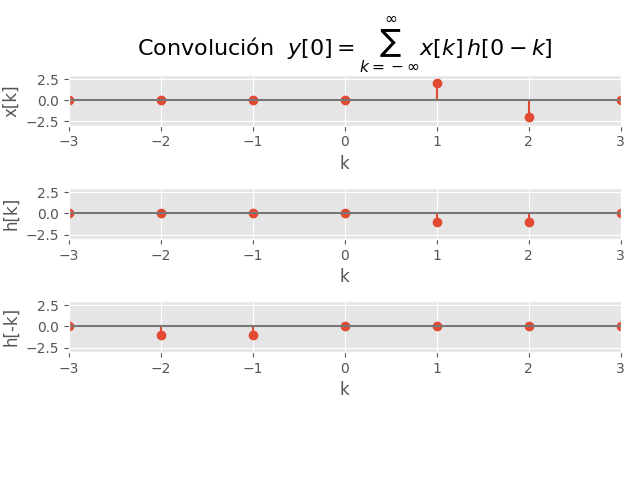
\includegraphics[width=6in]{./graphics/convejemp01-01.png}
	\caption{Señales $x[k]$, $h[k]$ y $h[-k]$.}
	\label{fig:convejemp0101}
\end{figure}

\begin{figure}[htbp]
	\centering
	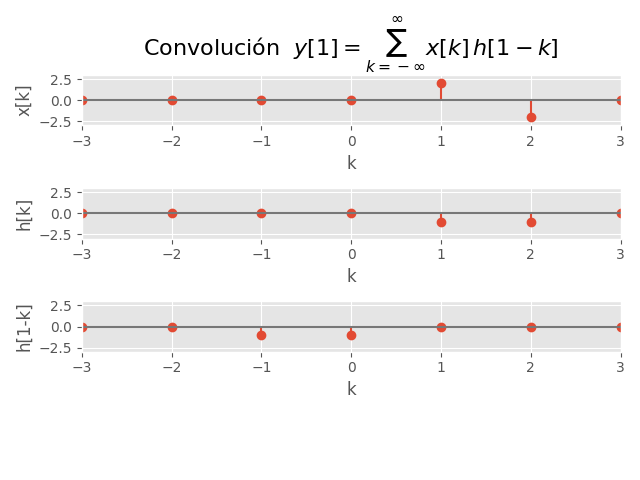
\includegraphics[width=6in]{./graphics/convejemp01-02.png}
	\caption{Señales $x[k]$, $h[k]$ y $h[1-k]$.}
	\label{fig:convejemp0102}
\end{figure}

\begin{figure}[htbp]
	\centering
	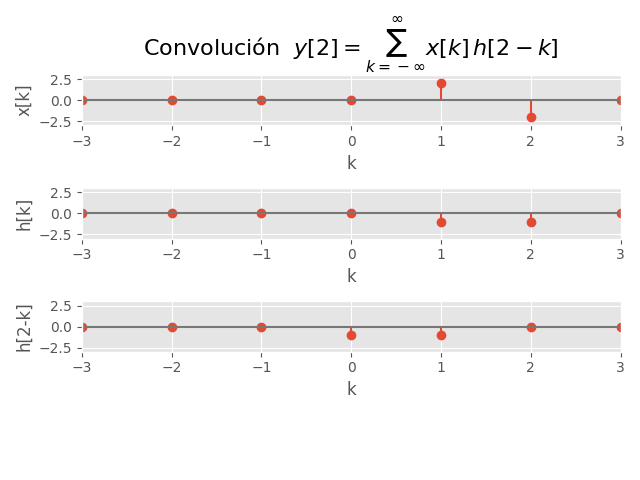
\includegraphics[width=6in]{./graphics/convejemp01-03.png}
	\caption{Señales $x[k]$, $h[k]$ y $h[2-k]$.}
	\label{fig:convejemp0103}
\end{figure}

\begin{figure}[htbp]
	\centering
	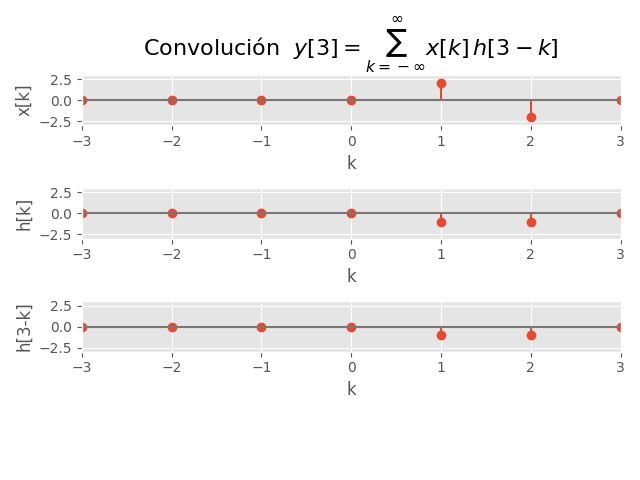
\includegraphics[width=6in]{./graphics/convejemp01-04.png}
	\caption{Señales $x[k]$, $h[k]$ y $h[3-k]$.}
	\label{fig:convejemp0104}
\end{figure}

\begin{figure}[htbp]
	\centering
	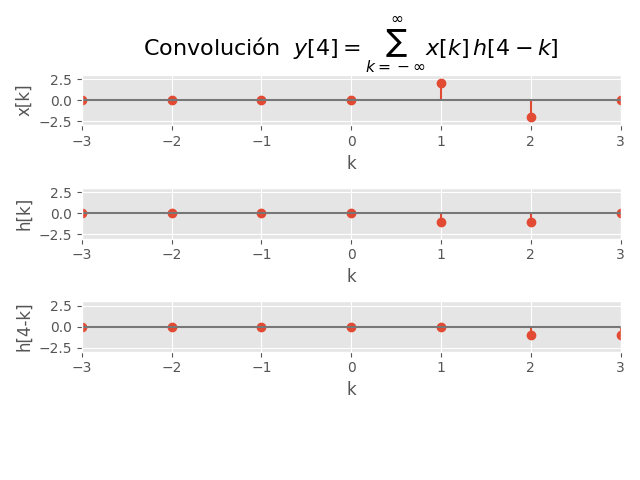
\includegraphics[width=6in]{./graphics/convejemp01-05.png}
	\caption{Señales $x[k]$, $h[k]$ y $h[4-k]$.}
	\label{fig:convejemp0105}
\end{figure}

\begin{figure}[htbp]
	\centering
	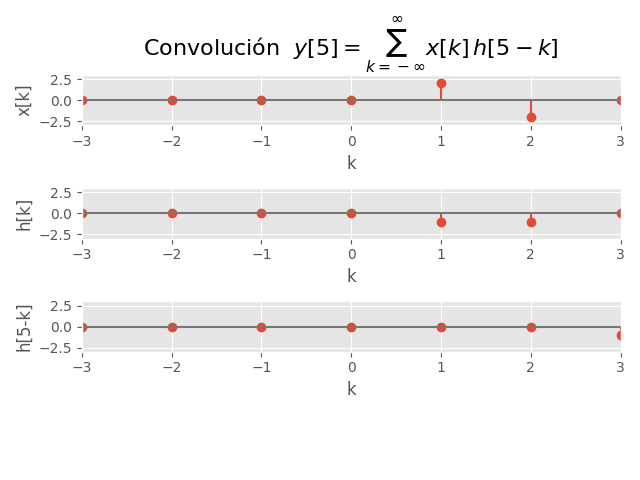
\includegraphics[width=6in]{./graphics/convejemp01-06.png}
	\caption{Señales $x[k]$, $h[k]$ y $h[5-k]$.}
	\label{fig:convejemp0106}
\end{figure}

\subsection{Convolución con un impulso}

Calculemos ahora la convolución de las señales:
\begin{align}
	x[n] &= \left( \frac{99}{100}\right)^n u[n], \\
	h[n] &= \delta[n-1].
\end{align}

\subsubsection{Forma gráfica}

\begin{enumerate}
	\item Dibujemos las señales $x[k]$, $h[k]$ y $h[-k]$.
	\item Dibujemos $h[n-k]$ para distintos valores de $n$, junto con $x[k]$. Ver Fig. (\ref{fig:convejemp0201}).
	\item Dibujemos el producto $z[n,k] = x[k] \, h[n-k]$.
	\item Calculemos $\sum_{k}z[n,k]$ para obtener $y[n]$.
\end{enumerate}

\begin{figure}[htbp]
	\centering
	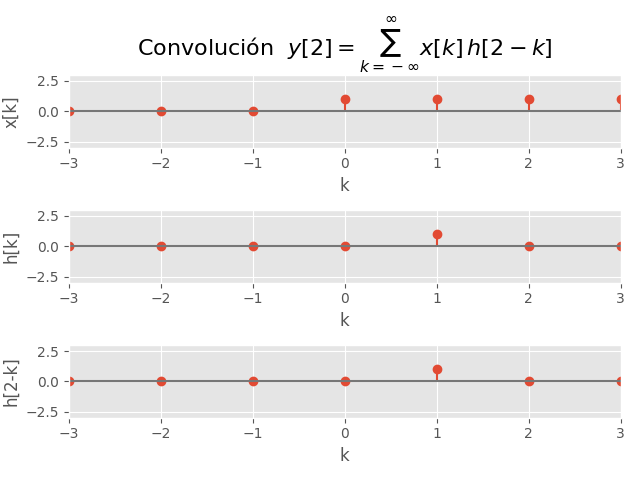
\includegraphics[width=6in]{./graphics/convejemp02-01.png}
	\caption{Señales $x[k]$, $h[k]$ y $h[2-k]$.}
	\label{fig:convejemp0201}
\end{figure}

\subsubsection{Forma analítica}

\begin{enumerate}
	\item Según la Ec. (\ref{convo}), tenemos:
	\begin{equation}
		y[n] = \sum_{k=-\infty}^{\infty} \left( \frac{99}{100}\right)^k u[k] \, \delta[n-1-k].
	\end{equation}
	
	\item Dado que dentro de la sumatoria aparece un escalón unitario, podemos eliminarlo modificando adecuadamente el límite inferior del índice $k$. Además, dado que la entrada contiene un factor escalón $u[n]$, la salida también tiene un factor similar. Entonces, como $u[k] = 0$ para $k < 0$, el límite inferior es $k = 0$, y además la sumatoria queda multiplicada por $u[n]$:
	\begin{equation}
		y[n] = \left(\sum_{k=0}^{\infty} \left( \frac{99}{100}\right)^k \delta[n-1-k] \right) \cdot u[n].
		\label{ejeconvimpulso.0}
	\end{equation}
	
	\item Observe que el índice del impulso es $n - 1 - k$, y que por lo tanto está ubicado en $k = n - 1$. Entonces:
	\begin{equation}
		\sum_{k=0}^{\infty}\left( \frac{99}{100}\right)^k \delta[n-1-k] = 
		\left( \frac{99}{100}\right)^{n-1} \delta[0] =
		\left( \frac{99}{100}\right)^{n-1}
		\label{ejeconvimpulso}
	\end{equation}
	
	\item Reemplazando (\ref{ejeconvimpulso}) en (\ref{ejeconvimpulso.0}), obtenemos:
	\begin{equation}
		y[n] = \left( \frac{99}{100}\right)^{n-1} \cdot u[n].
	\end{equation}
	
	\item En general, consideremos una respuesta al impulso:
	\begin{equation}
		h[n] = \delta[n-n_{0}].
	\end{equation}
	y calculemos su convolución para una entrada genérica $x[n]$.
	
	\item Según la Ec. (\ref{convo}), tenemos:
	\begin{equation}
		y[n] = \sum_{k=-\infty}^{\infty} x[k] \, \delta[n-n_{0}-k],
	\end{equation}
	
	\item Observe que el índice del impulso es $n - n_{0} - k$, y que por lo tanto está ubicado en $k = n - n_{0}$. Entonces:
	\begin{equation}
		x[k] \, \delta[n-n_{0}-k] = x[n-n_{0}] \, \delta[0] = x[n-n_{0}].
	\end{equation}
	
	\item Considerando la sumatoria, obtenemos:
	\begin{equation}
		\sum_{k=-\infty}^{\infty} x[n-n_{0}] \delta[n-n_{0}-k] = x[n-n_{0}].
	\end{equation}
	
	\item Dado que
	\begin{equation}
		u[n-n_{0}] = \left( \sum_{k=-\infty}^{\infty} \delta[n-n_{0}-k] \right)
	\end{equation}
	la salida $y[n]$ es:
	\begin{equation}
		y[n] = x[n-n_{0}] \, u[n-n_{0}].
	\end{equation}
\end{enumerate}

\subsection{Convolución de una señal con una ventana rectangular}

Calculemos la convolución de las señales:
\begin{align}
	x[n] &= \left( \frac{1}{2}\right)^n u[n], \\
	h[n] &= u[n] - u[n-2] = \delta[n] + \delta[n-1].
\end{align}

\subsubsection{Forma gráfica}

\begin{enumerate}
	\item Dibujemos las señales $x[k]$, $h[k]$ y $h[-k]$.
	\item Dibujemos $h[n-k]$ para distintos valores de $n$, junto con $x[k]$.
	\item Dibujemos el producto $z[n,k] = x[k] h[n-k]$.
	\item Calculemos $\sum_{k}z[n,k]$ para obtener $y[n]$.
\end{enumerate}

\subsubsection{Forma analítica}

\begin{enumerate}
	\item Según la Ec. (\ref{convo}), tenemos:
	\begin{equation}
		y[n] = \sum_{k=-\infty}^{\infty} \left( \frac{1}{2}\right)^k u[k] \, h[n-k].
	\end{equation}
	
	\item Ajustamos los índices de la sumatoria porque la señal es nula para $k < 0$:
	\begin{equation}
		y[n] = \sum_{k=0}^{\infty} \left( \frac{1}{2}\right)^k \, h[n-k].
	\end{equation}
	
	\item Expresamos a la ventana rectangular como una suma de impulsos desplazados en el tiempo:
	\begin{equation}
		y[n] = \sum_{k=0}^{\infty} \left( \frac{1}{2}\right)^k \left(\delta[n-k] + \delta[n-1-k] \right).
	\end{equation}
	
	\item Desdoblamos la convolución en dos:
	\begin{align}
		\sum_{k=0}^{\infty} \left( \frac{1}{2}\right)^k \, \delta[n-k] &= \left( \frac{1}{2}\right)^n u[n], \\
		\sum_{k=0}^{\infty} \left( \frac{1}{2}\right)^k \, \delta[n-1-k] &= \left( \frac{1}{2}\right)^{n-1} u[n-1].
	\end{align}
	
	\item El resultado final es:
	\begin{equation}
		y[n] = \left( \frac{1}{2}\right)^n u[n] + \left(\frac{1}{2}\right)^{n-1} u[n-1].
	\end{equation}
\end{enumerate}

\subsection{Convolución de señales infinitas}

Considere una entrada $x[n]$ y una respuesta al impulso unitario dadas por:
\begin{align}
	x[n] &= \alpha^n u[n], \\
	h[n] &= u[n],
\end{align}
donde el valor absoluto de $\alpha$ es menor que $1$:
\begin{equation}
	0 < |\alpha| < 1.
\end{equation}

\subsubsection{Forma gráfica}

\begin{enumerate}
	\item Dibujemos las señales $x[k]$, $h[k]$ y $h[-k]$.
	\item Dibujemos $h[n-k]$ para distintos valores de $n$, junto con $x[k]$.
	\item Dibujemos el producto $z[n,k] = x[k] \, h[n-k]$.
	\item Calculemos $\sum_{k} z[n,k]$ para obtener una aproximación de $y[n]$.
\end{enumerate}

\subsubsection{Forma analítica}

\begin{enumerate}
	\item Según la Ec. (\ref{convo}), tenemos:
	\begin{equation}
		\alpha^{k} u[k] u[n-k] = \begin{cases}
			\alpha^k, & 0 \leq k \leq n, \\ 
			0, & (k < 0) \lor (k > n).
		\end{cases}
		\label{convinf}
	\end{equation}
	
	\item Para poder realizar esta sumatoria, debemos recordar sucesiones geométricas. Definamos la suma parcial:
	\begin{equation}
		S_{n} = \sum_{k=0}^n \alpha^k,
	\end{equation}
	y multipliquemos por $\alpha$ para obtener:
	\begin{equation}
		\alpha \, S_{n} = \sum_{k=0}^n \alpha^{k+1}.
	\end{equation}
	Entonces podemos escribir:
	\begin{equation}
		S_{n} - \alpha \, S_{n} = \left( \sum_{k=0}^n \alpha^k \right) - \left( \sum_{k=0}^n \alpha^{k+1} \right)
	\end{equation}
	y simplificando:
	\begin{equation}
		S_n - \alpha \, S_n = \alpha^0 - \alpha^{n+1}.
	\end{equation}
	Podemos despejar entonces:
	\begin{equation}
		S_n = \frac{\alpha^0 - \alpha^{n+1}}{1-\alpha} = \frac{1-\alpha^{n+1}}{1-\alpha}.
		\label{sumageo}
	\end{equation}
	
	\item Aplicamos la Ec. (\ref{sumageo}) a la Ec. (\ref{convinf}):
	\begin{equation}
		\sum_{k=0}^n \alpha^k = \frac{1-\alpha^{n+1}}{1-\alpha}.
		\label{sumaserie}
	\end{equation}
	Por lo tanto, la respuesta es:
	\begin{equation}
		y[n] = \left( \frac{1-\alpha^{n+1}}{1-\alpha} \right) u[n].
	\end{equation}
\end{enumerate}

\subsection{Convolución de una señal consigo misma}

Vamos a calcular la convolución de una señal consigo misma, definiendo:
\begin{align}
	x[n] &= \left( \frac{8}{10}\right)^n u[n], \\
	h[n] &= \left( \frac{8}{10}\right)^n u[n].
\end{align}

\subsubsection{Forma gráfica}

\begin{enumerate}
	\item Dibujemos las señales $x[k]$, $h[k]$ y $h[-k]$.
	\item Dibujemos $h[n-k]$ para distintos valores de $n$, junto con $x[k]$.
	\item Dibujemos el producto $z[n,k] = x[k] h[n-k]$.
	\item Calculemos $\sum_{k}z[n,k]$ para obtener $y[n]$ en forma aproximada.
\end{enumerate}

\subsubsection{Forma analítica}

\begin{enumerate}
	\item Según la Ec. (\ref{convo}), tenemos:
	\begin{equation}
		y[n] = \sum_{k=-\infty}^{\infty} \left( \frac{8}{10}\right)^k u[k] \left( \frac{8}{10}\right)^{n-k} u[n-k].
	\end{equation}
	
	\item Podemos modificar los límites de la sumatoria, pues $u[k] = 0$ para $k < 0$, y $u[n-k] = 0$ para $n - k < 0$:
	\begin{equation}
		y[n] = \left( \sum_{k=0}^{n} \left( \frac{8}{10}\right)^{k+n-k} \right) \cdot u[n].
	\end{equation}
	Observe que si uno de los factores de la entrada es un escalón $u[n - n_{0}]$, la salida también tiene el mismo factor.
	
	\item Extraemos de la sumatoria el factor común de todos los sumandos $\left(\frac{8}{10}\right)^n$, que es independiente de $k$, y obtenemos:
	\begin{equation}
		y[n] = \left( \left( \frac{8}{10}\right)^n \sum_{k=0}^{n} 1 \right) \cdot u[n].
	\end{equation}
	
	\item Finalmente resulta esto:
	\begin{equation}
		y[n] = \left( \frac{8}{10}\right)^n \, (n+1) \, u[n].
	\end{equation}
	El factor $u[n]$ aparece porque la sumatoria cuyo resultado es $n + 1$ tiene un límite inferior $k = 0$, y por lo tanto la sumatoria es no nula si y solo si $n \geq 0$.
\end{enumerate}	
	
\chapter{Sistemas LIT en tiempo discreto}

\section{Introducción}

Hemos visto que la suma de convolución 
\begin{equation}
	y[n] = \sum_{k=-\infty}^{\infty} x[k] \, h[n-k] = x[n] * h[n] ,
\end{equation}
define la respuesta $y$ de un sistema LIT para una entrada $x$ si conocemos la respuesta al impulso $h$. Por lo tanto, en este capítulo usaremos la convolución como herramienta para estudiar distintas propiedades de los sistemas LIT.

\section{Propiedades de los sistemas LIT}

\subsection{La propiedad conmutativa}

El resultado de la convolución es independiente del ordenamiento de las señales, o en otras palabras, un sistema LIT de respuesta al impulso $h$ excitado con una entrada $x$ genera una salida similar al de un sistema LIT de respuesta al impulso $x$ excitado con una entrada $h$.

Consideremos la operación de convolución:
\begin{equation}
	y[n] = \sum_{k=-\infty}^{\infty} x[k] \, h[n-k] = \sum_{k=-\infty}^{\infty} h[k] \, x[n-k].
\end{equation}

Realizamos un cambio de variable $m = n - k$ y por consecuencia definimos $k = n - m$ para obtener:
\begin{equation}
	y[n] = \sum_{k=-\infty}^{\infty} x[k] \, h[n-k] = \sum_{m=-\infty}^{\infty} x[n-m] \, h[m].
\end{equation}

\subsection{La propiedad distributiva}

La salida de un sistema LIT cuya respuesta al impulso es $h_{a} + h_{b}$ para una entrada $x$ es similar a la suma de las salidas de dos sistemas de respuestas al impulso $h_{a}$ y $h_{b}$ frente a una entrada $x$.

Probaremos la distributividad de la convolución discreta:
\begin{align}
	y[n] &= x[n] * \left( h_{a}[n] + h_{b}[n] \right) , \\
	y[n] &= x[n] * h_{a}[n] + x[n] * h_{b}[n],
\end{align}
planteando:
\begin{equation}
	y[n] = \sum_{k=-\infty}^{\infty} x[k] \, \left( h_{a}[n-k] + h_{b}[n-k] \right).
\end{equation}
Dado que la multiplicación es distributiva respecto a la suma, obtenemos:
\begin{equation}
	y[n] = \sum_{k=-\infty}^{\infty} \left( x[k] \, h_{a}[n-k] + x[k] \, h_{b}[n-k] \right).
\end{equation}
Separando sumatorias:
\begin{equation}
	y[n] = \sum_{k=-\infty}^{\infty} \left( x[k] \, h_{a}[n-k] \right) + \sum_{k=-\infty}^{\infty} \left( x[k] \, h_{b}[n-k] \right) ,
\end{equation}
obtenemos:
\begin{equation}
	y[n] = x[n] * h_a[n] + x[n] * h_{b}[n] .
\end{equation}

\subsection{La propiedad asociativa}

La operación de convolución es asociativa:
\begin{align}
	y[n] &= x[n] * \left( h_a[n] * h_{b}[n] \right) , \\
	y[n] &= \left( x[n] * h_a[n] \right) * h_{b}[n] , \\
	y[n] &= x[n] * h_a[n] * h_{b}[n].
\end{align}

Para probar la propiedad asociativa, planteamos las dos formas de hacer el cálculo. Primero consideremos:
\begin{align}
	y_{1}[n] &= \sum_{p=-\infty}^{\infty} x[p] \, h_{a}[n-p], \\
	y[n] &= \sum_{q=-\infty}^{\infty} y_{1}[q] \, h_{b}[n-q].
\end{align}
Sustituyendo $y_1[q]$:
\begin{equation}
	y[n] = \sum_{q=-\infty}^{\infty} \left( \sum_{p=-\infty}^{\infty} x[p] \, h_{a}[q-p] \right) \, h_{b}[n-q],
\end{equation}
y reordenando:
\begin{equation}
	y[n] = \sum_{q=-\infty}^{\infty} \sum_{p=-\infty}^{\infty} x[p] \, h_{a}[q-p] \, h_{b}[n-q]. \label{eq:asoc1}
\end{equation}

Después consideramos el cálculo alternativo:
\begin{align}
	h[n] &= \sum_{r=-\infty}^{\infty} h_{a}[r] \, h_{b}[n-r], \\
	y[n] &= \sum_{s=-\infty}^{\infty} x[s] \, h[n-s].
\end{align}
Sustituyendo $h[n-s]$:
\begin{equation}
	y[n] = \sum_{s=-\infty}^{\infty} x[s] \, \left( \sum_{r=-\infty}^{\infty} h_{a}[r] \, h_{b}[n - s - r] \right),
\end{equation}
y reordenando:
\begin{equation}
	y[n] = \sum_{s=-\infty}^{\infty} \sum_{r=-\infty}^{\infty} x[s] \, h_{a}[r] \, h_{b}[n - s - r]. \label{eq:asoc2}
\end{equation}

Comparando (\ref{eq:asoc1}) y (\ref{eq:asoc2}), y considerando los cambios de variable $p = s$ y $q - p = r$ (lo que implica $q = r + s$), vemos que:
\begin{equation}
	n - q = n - (r + s) = n - s - r, 
\end{equation}
por lo tanto, ambas expresiones son idénticas, demostrando la propiedad.

\subsection{Preguntas}

\begin{enumerate}
	\item ¿Qué significado tiene la propiedad conmutativa de los sistemas lineales?
	\item ¿Qué significado tiene la propiedad distributiva de los sistemas lineales?
	\item ¿Qué significado tiene la propiedad asociativa de los sistemas lineales?
	\item Dé algún ejemplo concreto de estas tres propiedades.
\end{enumerate}

\subsection{Sistemas LIT con y sin memoria}

Un sistema no tiene memoria si su salida en cualquier momento depende solamente de la entrada de ese momento. Si un sistema no tiene memoria entonces debe ser $h[n]=0$ para todo $n \neq 0$, y por lo tanto:
\begin{equation}
	h[n] = K \, \delta[n] .
\end{equation}
Si un sistema tiene una respuesta al impulso $h[n]$ que es distinta de $0$ para $n \neq 0$, entonces el sistema tiene memoria.

\subsection{Preguntas}

\begin{enumerate}
	\item ¿Conoce algún sistema físico que no tenga memoria?
	\item ¿Conoce algún sistema físico que tenga memoria?
\end{enumerate}

\subsection{Sistemas LIT causales}

Si $y[n_{0}]$ no depende de $x[n]$ para $n > n_{0}$, entonces un sistema LIT es causal. Entonces todos los valores $h[n]$ para $n < 0$ deben ser $0$ y por lo tanto en la suma de convolución podemos cambiar el límite superior:
\begin{equation}
	y[n] = \sum_{k=-\infty}^{n} x[k] \, h[n-k],
\end{equation}
porque $h[n-k] = 0$ cuando $n - k < 0$, es decir, cuando $k > n$.

Además, si la entrada $x[n]$ comienza en $n = 0$ (es decir, $x[n]=0$ para $n<0$), podemos cambiar el límite inferior de la sumatoria:
\begin{equation}
	y[n] = \sum_{k=0}^{n} x[k] \, h[n-k].
\end{equation}
Esta fórmula significa que podemos calcular la salida de un sistema LIT causal con entrada causal de tiempo discreto con una cantidad finita de multiplicaciones y sumas.

\subsection{Preguntas}

Indicar si las siguientes afirmaciones son verdaderas o falsas, en el caso de un sistema lineal invariante en el tiempo:

\begin{enumerate}
	\item Si la entrada es nula para todo tiempo, entonces la salida es nula para todo tiempo.
	\item Si la relación entre entrada y salida es $y[n] = x[n] \, \cos(n)$, entonces el sistema es LIT.
	\item Si la relación entre entrada y salida es $y[n] = \sum_{k=0}^{n} x[k]$, entonces el sistema es LIT.
\end{enumerate}

\subsection{Sistemas LIT estables e inestables}

\subsubsection{Estabilidad BIBO}

El criterio de estabilidad \textbf{BIBO} (Bounded Input Bounded Output o entrada acotada, salida acotada) se puede expresar matemáticamente estableciendo que si la entrada está acotada por una constante $M_x < \infty$:
\begin{equation}
	|x[n]| \leq M_{x},
\end{equation}
entonces la salida debe estar acotada por una constante finita $M_y < \infty$:
\begin{equation}
	|y[n]| \leq M_{y}.
\end{equation}

Sustituyendo la suma de convolución y aplicando la desigualdad triangular (el valor absoluto de una suma es menor o igual a la suma de los valores absolutos), obtenemos:
\begin{equation}
	|y[n]| = \left| \sum_{k=-\infty}^{\infty} x[k] \, h[n-k] \right| \leq \sum_{k=-\infty}^{\infty} |x[k]| \, |h[n-k]|.
\end{equation}
Dado que $|x[k]| \leq M_x$ para todo $k$, podemos extraer la cota de la sumatoria:
\begin{equation}
	|y[n]| \leq M_{x} \sum_{k=-\infty}^{\infty} |h[n-k]|.
\end{equation}
Realizando el cambio de variable $m = n-k$, la sumatoria de $|h[n-k]|$ es idéntica a la sumatoria de $|h[m]|$. Para que la salida esté siempre acotada ($|y[n]| \leq M_{y} < \infty$), se debe cumplir que la suma de los valores absolutos de la respuesta al impulso sea finita:
\begin{equation}
	\sum_{m=-\infty}^{\infty} |h[m]| < \infty.
\end{equation}
A esto se lo conoce como una respuesta al impulso "absolutamente sumable".

\subsection{Respuesta de un sistema LIT en tiempo discreto a una entrada exponencial compleja}

\begin{enumerate}
	\item Vamos a calcular la convolución de una entrada $x[n] = e^{j \, \omega \, n}$ con una respuesta al impulso $h[n]$.
	\item Comenzamos escribiendo la fórmula alternativa de la suma de convolución:
	\begin{equation}
		y[n] = \sum_{k=-\infty}^{\infty} h[k] \, x[n-k].
	\end{equation}
	\item Sustituyendo $x[n - k] =  e^{j \, \omega \, (n-k)}$ obtenemos:
	\begin{equation}
		y[n] = \sum_{k=-\infty}^{\infty} h[k] \, e^{j \, \omega \, (n-k)} = \sum_{k=-\infty}^{\infty} h[k] \, e^{-j \, \omega \, k} \, e^{j \, \omega \, n}. \label{dt.eigenfunc.1}
	\end{equation}
	\item Viendo la ecuación (\ref{dt.eigenfunc.1}) podemos extraer el factor común $e^{j \, \omega \, n}$ de la sumatoria (ya que no depende de $k$) y escribir:
	\begin{equation}
		y[n] = \left(\sum_{k=-\infty}^{\infty} h[k] \, e^{-j \, \omega \, k}\right) \, e^{j \, \omega \, n}. \label{dt.eigenfunc.2}
	\end{equation}
	\item Viendo la ecuación (\ref{dt.eigenfunc.2}), podemos definir $H(e^{j \, \omega})$, la transformada de Fourier en tiempo discreto de $h[n]$:
	\begin{equation}
		H(e^{j \, \omega}) = \sum_{k=-\infty}^{\infty} h[k] \, e^{-j \, \omega \, k}. \label{dt.eigenfunc.3}
	\end{equation}	 
	\item Entonces resulta:
	\begin{equation}
		y[n] = H(e^{j \, \omega}) \, e^{j \, \omega \, n}.
	\end{equation}
	Se dice que las funciones de la forma $e^{j \, \omega \, n}$ son \textit{autofunciones} (o funciones propias) de los sistemas lineales invariantes en el tiempo, siendo $H(e^{j \, \omega})$ su autovalor correspondiente.
\end{enumerate}  

\subsection{Respuestas}

Estas son las respuestas a las preguntas planteadas arriba:

\begin{enumerate}
	\item ¿Qué significado tiene la propiedad conmutativa de los sistemas lineales?
	Un sistema LIT con respuesta al impulso $h[n]$ responde a una entrada $x[n]$ igual que un sistema LIT con respuesta al impulso $x[n]$ responde a una entrada $h[n]$. Además, cuando conectamos en serie dos sistemas LIT, no importa el orden en que se conecten: el conjunto de los dos sistemas va a responder igual ante cualquier entrada.
	
	\item ¿Qué significado tiene la propiedad distributiva de los sistemas lineales?
	Podemos implementar un sistema LIT con respuesta al impulso $h_{1}[n] + h_{2}[n]$ conectando en paralelo dos sistemas LIT cuyas respectivas respuestas al impulso sean $h_{1}[n]$ y $h_{2}[n]$.
	
	\item ¿Qué significado tiene la propiedad asociativa de los sistemas lineales?
	Cuando conectamos en cascada (serie) sistemas LIT, podemos agruparlos para formar nuevos sistemas LIT equivalentes sin alterar la salida final.
	
	\item ¿Conoce algún sistema físico que no tenga memoria?
	Un cable o un divisor resistivo ideal.
	
	\item ¿Conoce algún sistema físico que tenga memoria?
	Un tanque de agua (acumula o "recuerda" el agua que entra) o un capacitor en un circuito eléctrico.
	
	\item ¿La siguiente afirmación es verdadera o falsa? "Si la entrada es nula para todo tiempo, entonces la salida es nula para todo tiempo."
	\textbf{Verdadero}, pues si la entrada es nula, todos los productos en la suma de convolución son nulos.
	
	\item ¿La siguiente afirmación es verdadera o falsa? "Si la relación entre entrada y salida es $y[n] = x[n] \, \cos(n)$, entonces el sistema es LIT."
	\textbf{Falso}, porque el sistema varía en el tiempo. La respuesta a un impulso depende del instante de tiempo en el que este ocurra:
	\begin{equation}
		y[n] = \delta[n - n_{0}] \, \cos(n_{0}).
	\end{equation}
	
	\item ¿La siguiente afirmación es verdadera o falsa? Si la relación entre entrada y salida es $y[n] = \sum_{k=0}^{n} x[k]$, entonces el sistema es LIT.
	\textbf{Verdadero}, pues dicha relación puede escribirse como la convolución de la entrada con un escalón unitario $h[n] = u[n]$:
	\begin{equation}
		y[n] = \sum_{k=-\infty}^{\infty} x[k] \, u[k] \, u[n-k].
	\end{equation}
\end{enumerate}
	

\chapter{La integral de convolución}

\section{Deducción de la fórmula}

A continuación calculamos la salida $y(t)$ para una entrada arbitraria $x(t)$ en función de la respuesta al impulso $h(t)$ del sistema lineal invariante en el tiempo.

\subsection{Una señal como límite de una sumatoria}

\begin{figure}[htbp]
	\centering
	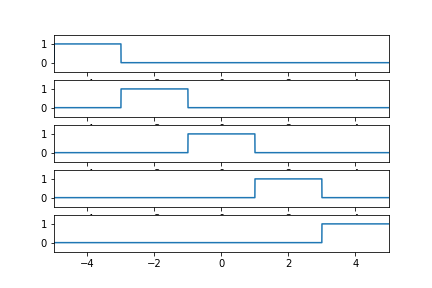
\includegraphics[width=0.7\linewidth]{graphics/pulses.png}
	\caption{Pulsos desplazados en el tiempo}
	\label{fig:pulses}
\end{figure}

\begin{figure}[htbp]
	\centering
	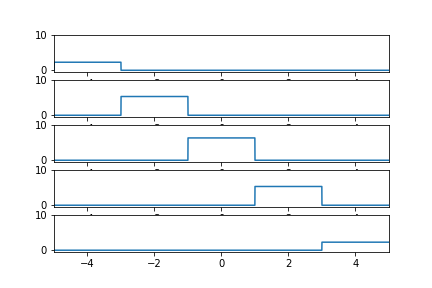
\includegraphics[width=0.7\linewidth]{graphics/modulated_pulses.png}
	\caption{Pulsos desplazados en el tiempo y modulados}
	\label{fig:modulatedpulses}
\end{figure}

\begin{figure}[htbp]
	\centering
	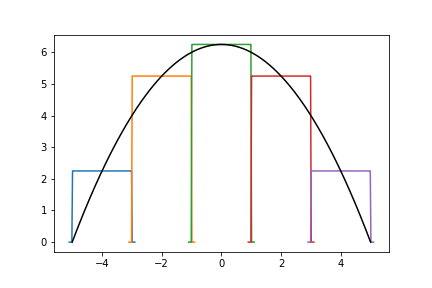
\includegraphics[width=0.7\linewidth]{graphics/coarse-approximation.png}
	\caption{Aproximación grosera}
	\label{fig:coarse-approximation}
\end{figure}

\begin{figure}[htbp]
	\centering
	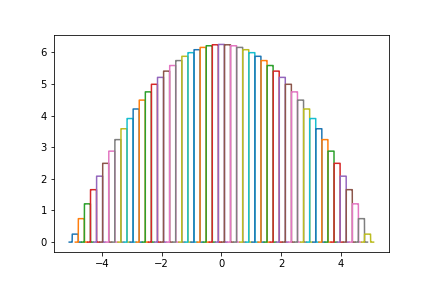
\includegraphics[width=0.7\linewidth]{graphics/fine-approximation.png}
	\caption{Aproximación fina}
	\label{fig:fine-approximation}
\end{figure}

Vamos a probar que podemos representar una señal continua como el límite de una suma de pulsos. Consideremos pulsos desplazados en el tiempo $\delta_{\Delta}\left(t - k \, \Delta \right)$ donde $\Delta$ es un incremento de tiempo variable.

Observando la figura \ref{fig:pulses}, podemos escribir las definiciones de los pulsos desplazados en el tiempo:
\begin{align}
	\vdots \nonumber \\ 
	\delta_{\Delta}(t+\Delta) &= \begin{cases}
		\frac{1}{\Delta}, & -\Delta \leq t < 0, \\ 
		0, & (t < -\Delta) \lor (0 \leq t).
	\end{cases} \\ 
	\delta_{\Delta}(t) &= \begin{cases}
		\frac{1}{\Delta}, & 0 \leq t < \Delta, \\ 
		0, & (t < 0) \lor (\Delta \leq t).
	\end{cases} \\ 
	\delta_{\Delta}(t-\Delta) &= \begin{cases}
		\frac{1}{\Delta}, & \Delta \leq t < 2\Delta, \\ 
		0, & (t < \Delta) \lor (2\Delta \leq t).
	\end{cases} \\ 
	\vdots \nonumber \\ 
	\delta_{\Delta}(t-k\Delta) &= \begin{cases}
		\frac{1}{\Delta}, & k\Delta \leq t < (k+1)\Delta, \\ 
		0, & (t < k\Delta) \lor ((k+1)\Delta \leq t).
	\end{cases}
\end{align}

Multiplicando por $x(k \, \Delta) \, \Delta$ al $k$-ésimo pulso (ver figura \ref{fig:modulatedpulses}) se obtiene:
\begin{align}
	\vdots \nonumber \\ 
	x(-\Delta) \, \delta_{\Delta}(t+\Delta) \, \Delta &= \begin{cases}
		\frac{x(-\Delta)}{\Delta} \, \Delta, & -\Delta \leq t < 0, \\ 
		0, & (t < -\Delta) \lor (0 \leq t).
	\end{cases} \\ 
	x(0) \, \delta_{\Delta}(t) \, \Delta &= \begin{cases}
		\frac{x(0)}{\Delta} \, \Delta, & 0 \leq t < \Delta, \\ 
		0, & (t < 0) \lor (\Delta \leq t).
	\end{cases} \\ 
	x(\Delta) \, \delta_{\Delta}(t-\Delta) \, \Delta &= \begin{cases}
		\frac{x(\Delta)}{\Delta} \, \Delta, & \Delta \leq t < 2\Delta, \\ 
		0, & (t < \Delta) \lor (2\Delta \leq t).
	\end{cases} \\ 
	\vdots \nonumber \\ 
	x(k\Delta) \, \delta_{\Delta}(t-k\Delta) \, \Delta &= \begin{cases}
		\frac{x(k\Delta)}{\Delta} \, \Delta, & k\Delta \leq t < (k+1)\Delta, \\ 
		0, & (t < k\Delta) \lor ((k+1)\Delta \leq t).
	\end{cases}
\end{align}

Observe que un valor dado de $t$ (por ejemplo $t_{0}$) sólo puede pertenecer a \textbf{un} intervalo $k\Delta \leq t < (k+1)\Delta$, por lo tanto, para $t_{0}$ solo uno de los productos puede ser distinto de $0$. Sumando los infinitos productos (ver figura \ref{fig:coarse-approximation}) obtenemos:
\begin{equation}
	x_{\Delta}(t) = \sum_{k=-\infty}^{\infty} x(k\Delta) \, \delta_{\Delta}(t-k\Delta) \, \Delta .
\end{equation}

Considerando la suma de los pulsos desplazados en el tiempo, podemos observar que cuando $\Delta$ tiende a cero (ver figura \ref{fig:fine-approximation}), $x_{\Delta}(t)$ tiende a $x(t)$.
\begin{equation}
	x(t) = \lim_{\Delta \to 0} x_{\Delta}(t) = \lim_{\Delta \to 0} \sum_{k=-\infty}^{\infty} x(k \, \Delta) \, \delta_{\Delta}(t-k \, \Delta) \, \Delta .
\end{equation}
Además, cuando $\Delta$ tiende a cero, la sumatoria se convierte en una integral:
\begin{equation}
	x(t) = \int_{-\infty}^{\infty} x(\tau) \, \delta(t-\tau) \, d\tau . \label{integral.convolucion}
\end{equation}

Notemos que por la propiedad del muestreo del impulso, debe cumplirse:
\begin{equation} 
	x(\tau) \, \delta(t-\tau) = x(t) \, \delta(t-\tau),
\end{equation}
y en ese caso:
\begin{equation}
	x(t) = x(t) \left( \int_{-\infty}^{\infty} \delta(t-\tau) \, d\tau \right).
\end{equation}

\subsection{La respuesta al impulso y la convolución}

Definamos $h_{k \, \Delta }(t) = h_{\Delta}\left( t-k \, \Delta \right)$ como la salida de un sistema invariante en el tiempo para el pulso $\delta_{\Delta}(t-k \, \Delta)$. 

Además, recordemos la ecuación (\ref{integral.convolucion}):
\begin{equation}
	x_{\Delta}(t) = \sum_{k=-\infty}^{\infty} x(k \, \Delta) \, \delta_{\Delta}(t-k \, \Delta) \, \Delta .
\end{equation}

La salida $y_{\Delta}(t)$ para una entrada $x_{\Delta}(t)$ puede definirse, por el principio de superposición, como:
\begin{equation}
	y_{\Delta}(t) = \sum_{k=-\infty}^{\infty} x(k\Delta) \, h_{k\Delta}(t) \, \Delta.
\end{equation}

Definamos $k\Delta = \tau$. Entonces, cuando $\Delta \to 0$, obtenemos como límite la señal $y(t)$, pero como siempre vamos a tener un $k$ suficientemente grande, $\tau$ no es necesariamente nula. Podemos escribir:
\begin{equation}
	y(t) = \lim_{\Delta \to 0} \sum_{k=-\infty}^{\infty} x(k \, \Delta) \, h_{k\Delta}(t) \, \Delta = \int_{-\infty}^{\infty} x(\tau) \, h_{\tau}(t) \, d\tau .
\end{equation}

Si el sistema es invariante en el tiempo, entonces:
\begin{equation}
	h_{\tau}(t) = h_{0}(t-\tau) ,
\end{equation}
(es decir, no importa para qué $\tau$ calculamos la respuesta, y por lo tanto elegimos $\tau=0$). Reemplazando $h_0$ simplemente por $h$, obtenemos la \textbf{integral de convolución}:
\begin{equation}
	y(t) = \int_{-\infty}^{\infty} x(\tau) \, h(t-\tau) \, d\tau .
\end{equation}

\section{Cálculo de la integral de convolución en forma gráfica}


El cálculo de la convolución tiene una interpretación gráfica.
\begin{enumerate}
	\item Consideremos la fórmula, utilizando $v$ como variable muda de integración:
	\begin{equation}
		y(t) = \int_{-\infty}^{\infty} x(v) \, h(t - v) \, dv. \label{concontgraf}
	\end{equation}
	
	\item En la Ec. (\ref{concontgraf}), el factor $h(t - v)$ es una versión de $h(v)$ invertida en el tiempo (observe el signo de la variable $v$) y desplazada por la variable independiente $t$, que es el instante para el cual deseamos calcular la salida $y(t)$.
	
	\item En base a la observación anterior, es posible enunciar la siguiente "receta" para calcular la convolución en forma gráfica:
	\begin{enumerate}
		\item Dibuje la señal $x(v)$.
		\item Invierta en el tiempo la señal $h(v)$ para obtener $h(-v)$.
		\item Repita los siguientes pasos para calcular distintos valores de $y(t)$:
		\begin{enumerate}
			\item Desplace en el tiempo la señal $h(-v)$ para obtener $h(t-v)$.
			\item Obtenga el producto $z(v,t) = x(v) \, h(t - v)$.
			\item El valor de $y(t)$ es el área bajo la curva $\int z(v,t) \, dv$.
		\end{enumerate}
	\end{enumerate}
\end{enumerate}

\section{Ejemplos}

\subsection{Convolución de una señal con un impulso desplazado}

Supongamos la entrada $x(t) = \delta(t-a)$ a un sistema lineal invariante en el tiempo con respuesta al impulso $h(t)$. En este caso la salida es:
\begin{equation}
	y(t) = \int_{-\infty}^{\infty} \delta(v - a) \, h(t - v) \, dv.
\end{equation}
Notemos que por la propiedad del impulso, el producto $\delta(v - a) \, h(t - v)$ es no nulo solo cuando $v = a$, es decir, $\delta(v - a) \, h(t - a)$. Por lo tanto:
\begin{equation}
	y(t) = \int_{-\infty}^{\infty} h(t - a) \, \delta(v - a ) \, dv = h(t - a) \left( \int_{-\infty}^{\infty} \delta(v - a ) \, dv \right).
\end{equation}
Recordemos que por definición de impulso:
\begin{equation}
	\int_{-\infty}^{\infty} \delta(v - a ) \, dv = 1.
\end{equation}
Por lo tanto:
\begin{equation}
	y(t) = h(t - a).
\end{equation}
Así comprobamos la invariancia en el tiempo de los sistemas cuya salida $y(t)$ para una entrada $x(t)$ puede calcularse con la integral de convolución.

\subsection{Dos señales infinitas}

\begin{enumerate}
	
	\item Sean dos señales definidas como:
	\begin{align}
		x(t) &= e^{2t} \, u(-t) ,  \\
		h(t) &= u(t-3).
	\end{align}
	
	\item Calculando la integral de convolución tenemos:
	\begin{equation}
		x(t) * h(t) = \int_{-\infty}^{\infty} e^{2\tau} u(-\tau) u(t-3-\tau) d\tau .
	\end{equation}
	
	\item El producto de los escalones $u(-\tau) u(t-3-\tau)$ puede analizarse así:
	\begin{enumerate}
		\item Debemos observar las transiciones de los escalones (donde cambian de $0$ a $1$ y viceversa). Estas transiciones determinan los límites de integración, porque si el integrando es nulo entonces la integral se anula.
		\item Sabemos que $u(-\tau) = 1$ para $\tau \leq 0$.
		\item Sabemos que $u(t-3-\tau) = 1$ para $\tau \leq t-3$.
		\item Por lo tanto, el integrando es no nulo cuando $\tau \leq \min(0, t-3)$.
	\end{enumerate}
	
	\item Evaluando para distintos valores de $t$:
	\begin{itemize}
		\item Para $t < 3$, el límite superior es $t-3$. 
		\begin{equation}
			x(t) * h(t) = \int_{-\infty}^{t-3} e^{2\tau} d\tau = \left[ \frac{1}{2}e^{2\tau} \right]_{-\infty}^{t-3} = \frac{1}{2}e^{2(t-3)}.
		\end{equation}
		
		\item Para $t \geq 3$, el límite superior es $0$.
		\begin{equation}
			x(t) * h(t) = \int_{-\infty}^{0} e^{2\tau} d\tau = \left[ \frac{1}{2}e^{2\tau} \right]_{-\infty}^{0} = \frac{1}{2}.
		\end{equation}
	\end{itemize}
	
\end{enumerate}

\subsection{Un par de señales limitadas en tiempo}

\begin{enumerate}
	
	\item Sean las señales:
	\begin{equation}
		x(t) = u(t) - u(t-4),
	\end{equation}
	y
	\begin{equation}
		h(t) = \cos\left( \frac{\pi t}{2}\right) \left( u(t) - u(t-4) \right).
	\end{equation}
	
	\item Planteando la integral de convolución (y aplicando la propiedad conmutativa para que el argumento complejo quede en el coseno), obtenemos:
	\begin{equation}
		x(t) * h(t) = \int_{-\infty}^{\infty} \cos\left( \frac{\pi \tau}{2}\right) \left( u(\tau) - u(\tau -4) \right) \left( u(t-\tau) - u(t-4-\tau) \right) d\tau .
	\end{equation}
	
	\item Analizando el solapamiento de ambas ventanas rectangulares de ancho 4, obtenemos los siguientes intervalos:
	\begin{align}
		t < 0, &\quad x(t) * h(t) = 0, \\
		0 \leq t < 4, &\quad x(t) * h(t) = \int_{0}^{t} \cos\left( \frac{\pi \tau}{2}\right) d\tau , \\
		4 \leq t < 8, &\quad x(t) * h(t) = \int_{t-4}^{4} \cos\left( \frac{\pi \tau}{2}\right) d\tau , \\
		t \geq 8, &\quad x(t) * h(t) = 0.
	\end{align}
	
\end{enumerate}

\subsection{Otro par de señales limitadas en tiempo}

\begin{enumerate}
	
	\item Sean dos señales definidas por:
	\begin{align}
		x(t) &= \begin{cases}
			1, & 0 \leq t < T, \\ 
			0, & (t < 0) \lor (t \geq T).
		\end{cases} \\
		h(t) &= \begin{cases}
			t, & 0 \leq t < T, \\ 
			0, & (t < 0) \lor (t \geq T).
		\end{cases}
	\end{align}
	En forma compacta usando escalones unitarios:
	\begin{align}
		x(t) &= u(t) - u(t-T) , \\
		h(t) &= t \, (u(t) - u(t-T)) .
	\end{align}
	
	\item Invirtiendo y desplazando en el tiempo una de las señales, tenemos:
	\begin{equation}
		h(t-\tau) = (t-\tau) \, (u(t-\tau) - u(t-\tau -T)) .
	\end{equation}
	
	\item Finalmente, calculamos la integral:
	\begin{equation}
		f(t) = \int_{-\infty}^{\infty} \left( u(\tau) - u(\tau-T) \right) (t-\tau) \left( u(t-\tau) - u(t-\tau-T) \right) d\tau.
	\end{equation}
	
	\item Al igual que en el ejemplo anterior, analizamos el solapamiento de la ventana $x(\tau)$ (entre $0$ y $T$) con la ventana deslizante $h(t-\tau)$ (entre $t-T$ y $t$), obteniendo la siguiente función a trozos:
	\begin{equation}
		f(t) = \begin{cases}
			0, & t < 0, \\
			\left[ t \tau - \frac{\tau^2}{2} \right]_{0}^{t} = \frac{t^2}{2}, & 0 \leq t < T, \\
			\left[ t \tau - \frac{\tau^2}{2} \right]_{t-T}^{T} = -\frac{t^2}{2} + tT, & T \leq t < 2T, \\
			0, & t \geq 2T.
		\end{cases}
	\end{equation}
	
\end{enumerate}

\chapter{Sistemas LIT y la integral de convolución}

% corresponde al archivo sys_2023/chapter-12.tex

\section{Introducción}

Hemos visto que la integral de convolución 
\begin{equation}
	y(t) = \int_{-\infty }^{\infty } x(\tau) \, h(t-\tau) \, d\tau = x(t) * h(t) ,
\end{equation}
define la respuesta $y(t)$ de un sistema LIT para una entrada $x(t)$ si conocemos la respuesta al impulso $h(t)$. Por lo tanto, en este capítulo usaremos la convolución como herramienta para estudiar distintas propiedades de los sistemas LIT en tiempo continuo.

\section{Propiedades de los sistemas LIT}

\subsection{La propiedad conmutativa}

El resultado de la convolución es independiente del ordenamiento de las señales, o en otras palabras, un sistema LIT de respuesta al impulso $h(t)$ excitado con una entrada $x(t)$ genera una salida similar a la de un sistema LIT de respuesta al impulso $x(t)$ excitado con una entrada $h(t)$.

Consideremos la operación de convolución:
\begin{equation}
	y(t) = \int_{-\infty }^{\infty } x(\tau) \, h(t-\tau) \, d\tau = \int_{-\infty }^{\infty } h(\tau) \, x(t-\tau) \, d\tau .
\end{equation}

Realizamos un cambio de variable $\upsilon = t - \tau$ y por consecuencia definimos $\tau = t - \upsilon$. Al cambiar los límites de integración (cuando $\tau \to \infty$, $\upsilon \to -\infty$), obtenemos:
\begin{equation}
	y(t) = -\int_{\infty }^{-\infty } x(t-\upsilon) \, h(\upsilon) \, d\upsilon = \int_{-\infty }^{\infty } x(t-\upsilon) \, h(\upsilon) \, d\upsilon .
\end{equation}

\subsection{La propiedad distributiva}

La salida de un sistema LIT cuya respuesta al impulso es $h_{a} + h_{b}$ para una entrada $x$ es similar a la suma de las salidas de dos sistemas con respuestas al impulso $h_{a}$ y $h_{b}$ frente a una entrada $x$.

Se puede probar la distributividad de la convolución respecto a la suma de señales:
\begin{align}
	y(t) &= x(t) * \left( h_a(t) + h_{b}(t) \right) , \\
	y(t) &= x(t) * h_a(t) + x(t) * h_{b}(t),
\end{align}
pues para la integral vale la siguiente propiedad de linealidad:
\begin{equation}
	\int_{a}^{b} x(v) \, (f(v) + g(v)) \, dv = \int_{a}^{b} x(v) \, f(v) \, dv + \int_{a}^{b} x(v) \, g(v) \, dv.
\end{equation}

\subsection{La propiedad asociativa}

Queda como ejercicio para el alumno la prueba de esta propiedad (similar a la demostración en tiempo discreto).
\begin{align}
	y(t) &= x(t) * \left( h_a(t) * h_{b}(t) \right) , \\
	y(t) &= \left( x(t) * h_a(t) \right) * h_{b}(t) , \\
	y(t) &= x(t) * h_a(t) * h_{b}(t) .
\end{align}

\subsection{Preguntas}

\begin{enumerate}
	\item ¿Qué significado tiene la propiedad conmutativa de los sistemas lineales?
	\item ¿Qué significado tiene la propiedad distributiva de los sistemas lineales?
	\item ¿Qué significado tiene la propiedad asociativa de los sistemas lineales?
	\item Dé algún ejemplo concreto de estas tres propiedades.
\end{enumerate}

\subsection{Sistemas LIT con y sin memoria}

Un sistema no tiene memoria si su salida en cualquier momento depende solamente de la entrada de ese mismo momento. Si un sistema no tiene memoria entonces su respuesta al impulso debe ser $h(t) = 0$ para todo $t \neq 0$, y por lo tanto toma la forma:
\begin{equation}
	h(t) = K \, \delta(t) .
\end{equation}
Si un sistema tiene una respuesta al impulso $h(t)$ que no es idénticamente cero para $t \neq 0$, entonces el sistema tiene memoria.

\subsection{Preguntas}

\begin{enumerate}
	\item ¿Conoce algún sistema físico que no tenga memoria?
	\item ¿Conoce algún sistema físico que tenga memoria?
\end{enumerate}

\subsection{Sistemas LIT causales y no causales}

Si $y(t)$ no depende de la entrada en instantes futuros ($x(t_{1})$ para $t_{1} > t$), entonces un sistema LIT es causal. Esto implica que la función $h(t-\tau)$ que multiplica a $x(\tau)$ debe ser cero para $\tau > t$, o sea que:
\begin{equation}
	h(t) = 0, \quad \text{para } t < 0.
\end{equation}
Por lo tanto, la integral de convolución para un sistema LIT causal restringe su límite superior:
\begin{equation}
	y(t) = \int_{-\infty}^{t} x(\tau) \, h(t-\tau) \, d\tau .
\end{equation}
Adicionalmente, si sabemos que la \textbf{entrada también es causal} (es decir, $x(t) = 0$ para $t < 0$), el límite inferior de la integral también se modifica, resultando en:
\begin{equation}
	y(t) = \int_{0}^{t} x(\tau) \, h(t-\tau) \, d\tau .
\end{equation}

\subsection{Sistemas LIT estables e inestables}

\subsubsection{Estabilidad BIBO}

El criterio de estabilidad \textbf{BIBO} (Bounded Input Bounded Output o entrada acotada, salida acotada) se puede expresar matemáticamente estableciendo que si la magnitud de la entrada está acotada por un valor finito:
\begin{equation}
	|x(t)| \leq M_{x} < \infty,
\end{equation}
entonces la salida debe estar acotada por un valor finito:
\begin{equation}
	|y(t)| \leq M_{y} < \infty.
\end{equation}

Analizando la integral de convolución y aplicando la desigualdad de valor absoluto, el sistema será estable si:
\begin{equation}
	|y(t)| = \left| \int_{-\infty }^{\infty } x(\tau) \, h(t-\tau) \, d\tau \right| \leq \int_{-\infty }^{\infty } |x(\tau)| \, |h(t-\tau)| \, d\tau .
\end{equation}
Dado que sabemos que $|x(\tau)| \leq M_x$, podemos extraer esta cota constante de la integral:
\begin{equation}
	|y(t)| \leq M_{x} \int_{-\infty }^{\infty } |h(t-\tau)| \, d\tau.
\end{equation}
Haciendo un cambio de variable $\upsilon = t - \tau$, la integral sobre todo el eje real no se ve alterada por el desplazamiento $t$. Para garantizar que la salida $|y(t)|$ siempre sea finita (menor que $M_y$), la integral del valor absoluto de la respuesta al impulso debe ser un valor finito:
\begin{equation}
	\int_{-\infty }^{\infty } |h(\tau)| \, d\tau < \infty.
\end{equation}
A esta condición necesaria y suficiente se la denomina poseer una respuesta al impulso \textbf{absolutamente integrable}.

\subsection{Preguntas}

\begin{enumerate}
	\item ¿Conoce algún sistema físico inestable?
	\item Dé ejemplos de sistemas estables e inestables.
	\item Indicar si las siguientes afirmaciones son verdaderas o falsas, en el caso de un sistema lineal invariante en el tiempo:
	\begin{enumerate}
		\item Si la entrada es nula para todo tiempo, entonces la salida es nula para todo tiempo.
		\item Si la relación entre entrada y salida es $y(t) = x(t) \cos(t)$, entonces el sistema es LTI.
		\item Si la relación entre entrada y salida es $y(t) = \int_{-\infty}^{t} x(\tau) \, d\tau$, entonces el sistema es LTI.
	\end{enumerate}
\end{enumerate}

\subsection{Respuestas a las afirmaciones}

\begin{enumerate}
	\item \textbf{Verdadero.} Si la entrada es nula ($x(t)=0$), la integral de convolución se evalúa como cero para todo $t$.
	
	\item \textbf{Falso.} Porque el sistema es variante en el tiempo. La respuesta a un impulso depende del instante de tiempo en que el impulso ocurre. Si aplicamos $x(t) = \delta(t - t_0)$, la salida será:
	\begin{equation}
		y(t) = \delta(t - t_{0}) \cos(t) = \delta(t - t_{0}) \cos(t_{0}).
	\end{equation}
	La amplitud del impulso de salida depende de cuándo se aplicó ($t_0$), lo cual viola la propiedad de invarianza.
	
	\item \textbf{Verdadero.} Dicha relación corresponde al comportamiento de un integrador ideal, el cual es un sistema LTI, y su salida puede escribirse formalmente como la convolución de la entrada con un escalón unitario $u(t)$:
	\begin{equation}
		y(t) = \int_{-\infty}^{t} x(\tau) \, d\tau = \int_{-\infty}^{\infty} x(\tau) \, u(t-\tau) \, d\tau = x(t) * u(t).
	\end{equation}
\end{enumerate}

	% ==========================================
	% BIBLIOGRAFÍA Y EJERCICIOS
	% ==========================================
	
	\cleardoublepage
	\phantomsection
	\addcontentsline{toc}{chapter}{Bibliografía y Ejercicios Recomendados}
	\chapter*{Bibliografía y Ejercicios Recomendados}
	
	\textbf{Bibliografía específica para este bloque:}
	\begin{itemize}
		\item \textbf{Oppenheim:} Capítulo 1 (Secciones 1.1 a 1.6) y Capítulo 2 (Secciones 2.1 a 2.4).
	\end{itemize}
	
	\textbf{Ejercicios recomendados:}
	\begin{itemize}
		\item Problemas de fin de capítulo 1.21 a 1.27 (propiedades de sistemas).
		\item Problemas de fin de capítulo 2.21 a 2.23 (convoluciones básicas).
	\end{itemize}
	
% ==========================================
% INICIO DEL BLOQUE II
% ==========================================

\part{Análisis de Fourier}

% ==========================================
% SEMANA 3
% ==========================================

\chapter{Series de Fourier (Tiempo continuo)}

\section{Motivación}

¿Para qué estudiamos series de Fourier? Veremos que es posible representar una señal de dos formas diferentes, una en el dominio del tiempo y otra en el dominio de la frecuencia. En otras palabras, podemos visualizar la señal de dos formas: una cuyo eje horizontal corresponde al tiempo, y otra cuyo eje horizontal corresponde a la frecuencia. En las dos representaciones tenemos la misma información.

La forma más sencilla de comenzar a trabajar en el dominio de la frecuencia es graficar los coeficientes de series de Fourier en función de las frecuencias de las armónicas de funciones periódicas. En las aplicaciones de procesamiento de señales y electrónica, nos interesa conocer la distribución de energía en función de la frecuencia.

\section{Definiciones}

Recordemos que una señal $x(t)$ es periódica si y sólo si existe el período, un número $T > 0$ que cumple con la condición:
\begin{equation}
	x(t) = x(t+T),
\end{equation}
para todo valor de $t$. Como ejemplos, veamos las siguientes funciones elementales y comprobemos su periodicidad:
\begin{align}
	x_1(t) &= \cos(\omega_0 \, t) = \cos\left(\omega_0 \left(t + \frac{2\pi}{\omega_0}\right)\right) = \cos(\omega_0 \, t + 2\pi), \\
	x_2(t) &= e^{j \omega_0 t} = e^{j \omega_0 \left(t + \frac{2\pi}{\omega_0}\right)} = e^{j \omega_0 t} e^{j 2\pi} = e^{j \omega_0 t}.
\end{align}

Para una señal periódica $x(t)$ con período fundamental $T = \frac{2\pi}{\omega_0}$, la representación en serie de Fourier (Ecuación de Síntesis) está dada por la suma ponderada de exponenciales complejas armónicamente relacionadas:
\begin{equation}
	x(t) = \sum_{k=-\infty}^{\infty} c_k \, e^{j k \omega_0 t}
\end{equation}
donde los coeficientes espectrales $c_k$ se calculan mediante la Ecuación de Análisis:
\begin{equation}
	c_k = \frac{1}{T} \int_{T} x(t) \, e^{-j k \omega_0 t} \, dt
\end{equation}

\section{Ejercicios}

% Signals and Systems with Matlab 2009, pages 65 - 67

\begin{enumerate}
	\item Obtenga coeficientes de Fourier (para una serie expresada como suma ponderada de exponenciales imaginarias) para una señal triangular obtenida integrando la señal cuadrada $x_{5}(t)$ definida previamente en la ecuación (\ref{squarewave}). Grafique el espectro correspondiente.
	
	\item Obtenga coeficientes de Fourier (para una serie expresada como suma ponderada de exponenciales imaginarias) para una señal triangular obtenida integrando la señal $x_{6}(t)$ definida en la ecuación (\ref{squarewaveone.1}). Grafique el espectro correspondiente.
	
	\item Obtenga coeficientes de Fourier (para una serie expresada como suma ponderada de exponenciales imaginarias) para el tren de pulsos rectangulares periódico de período $T$, tal que $0 < T_{1} \leq T$, definido en un período fundamental como:
	\begin{equation}
		x_{7}(t) = \begin{cases}
			1, & |t| \leq \frac{T_{1}}{2}, \\
			0, & \frac{T_{1}}{2} < |t| \leq \frac{T}{2}.
		\end{cases}
	\end{equation}
	Compruebe analíticamente que los coeficientes $c_k$ se pueden definir como una envolvente tipo "Sinc":
	\begin{equation}
		c_{k} = \frac{1}{T} \int_{-T_1/2}^{T_1/2} 1 \cdot e^{-j k \omega_0 t} \, dt = \frac{\sin\left(k \, \omega_0 \, \frac{T_{1}}{2}\right)}{k \, \pi} = \frac{T_1}{T} \text{sinc}\left(k \, \omega_0 \, \frac{T_1}{2}\right)
	\end{equation}
\end{enumerate}

\section{Serie de Fourier muestreada}

% Desarrollo de los siguientes temas:
% - Diferencia fundamental con CTFS (periodicidad de las exponenciales discretas, N coeficientes).
% - Ecuaciones de síntesis y análisis (sumatorias finitas).
% - Propiedades de la DTFS.
% - Sistemas LTI y Series de Fourier: Filtrado de señales periódicas.


% ==========================================
% SEMANA 4
% ==========================================

\chapter{Transformada de Fourier de tiempo continuo}

\section{Introducción}

\begin{enumerate}
	
	\item Vamos a ver como podemos \textbf{modificar} el concepto de \textbf{serie de Fourier} \textbf{para estudiar funciones no periódicas} de tiempo continuo. Esto nos permite \textbf{definir} el concepto de \textbf{contenido de frecuencias de una señal}, aún cuando sea no periódica.
	
	\item Pensemos en el ejemplo de un tren de pulsos simétrico, donde
	\begin{equation}
		a_{0} = \frac{T_{1}}{T_{2}},
	\end{equation}
	y
	\begin{equation}
		a_{k} = \frac{T_{1}}{T} \, \frac{\sin\left(\frac{k \, \pi \, T_{1}}{T}\right)}{\frac{k \, \pi \, T_{1}}{T}}. \label{tf.1}
	\end{equation}
	
	\item Podemos escribir (\ref{tf.1}) de la siguiente forma
	\begin{equation}
		T a_{k} = \left. T_{1} \, \frac{\sin(\omega)}{\omega} \right|_{\omega = \frac{k \, \pi \, T_{1}}{T}}
	\end{equation}
	y entonces es evidente que la podemos interpretar como una \textbf{secuencia} formada por \textbf{muestras} de una \textbf{función envolvente} $T_{1} \, \frac{\sin(\omega)}{\omega}$ donde la variable $\omega$ es continua, y la secuencia $T a_{k}$ está formada por valores igualmente espaciados en frecuencia, con intervalo $\frac{2 \, \pi}{T}$ (suponiendo $2T_1$ como el ancho del pulso).
	
	\item Observe que la separación de las muestras de la envolvente de $T a_{k}$ está dada por 
	\begin{equation}
		\omega_{T} = \frac{2 \, \pi}{T}.
	\end{equation}
	Entonces, cuanto mayor sea $T$ menor será $\omega_{T}$ y la cantidad de muestras en un intervalo dado de frecuencia será mayor.
	
	\item Si fijamos el valor del ancho del pulso (recordando que debe ser menor a $T$, por hipótesis) la envolvente de $T a_{k}$ es independiente de $T$.
	
\end{enumerate}

\section{Síntesis y análisis}

\subsection{Teoría}

\begin{enumerate}
	
	\item Vamos a construir una señal $x(t)$ no periódica como el límite de una señal $\hat{x}(t)$ periódica cuando el período $T$ tiende a $\infty$. Veamos qué pasa con los coeficientes de la serie de Fourier. Recordemos que una señal periódica $\hat{x}(t) = \hat{x}(t+T)$ se puede escribir como una serie de Fourier mediante la ecuación de síntesis 
	\begin{equation}
		\hat{x}(t) = \sum_{k=-\infty}^{\infty} a_{k} \, e^{j \, k \, \omega_{0} \, t},
	\end{equation}
	donde los coeficientes $a_{k}$ se calculan mediante la ecuación de análisis 
	\begin{equation}
		a_{k} = \frac{1}{T} \int_{-\frac{T}{2}}^{\frac{T}{2}} \hat{x}(t) e^{-j \, k \, \omega_{0} \, t} \, dt.
	\end{equation}
	
	\item Definamos la señal no periódica $x(t)$ especificando 
	\begin{equation}
		x(t) = \begin{cases}
			\hat{x}(t), & |t| \leq \frac{T}{2}, \\
			0, & |t| > \frac{T}{2},
		\end{cases}
		\qquad
		\hat{x}(t) = \hat{x}(t+T) .
	\end{equation}
	Entonces los coeficientes de la serie de Fourier son 
	\begin{equation}
		a_{k} = \frac{1}{T} \int_{-\frac{T}{2}}^{\frac{T}{2}} \hat{x}(t) e^{-j \, k \, \omega_{0} \, t} \, dt = \frac{1}{T} \int_{-\infty}^{\infty} x(t) e^{-j \, k \, \omega_{0} \, t} \, dt.
	\end{equation}
	\textbf{Las dos integrales son iguales en valor porque un período de $\hat{x}(t)$ coincide con $x(t),$ justamente donde se evalúa la primer integral, y $x(t)$ es nula para $|t| > \frac{T}{2}.$}
	
	\item Definamos la ecuación de análisis de la transformada de Fourier como 
	\begin{equation}
		X(j \, \omega) = \int_{-\infty}^{\infty} x(t) e^{-j \, \omega \, t} \, dt.
	\end{equation}
	Tenemos que los coeficientes de la serie de Fourier forman la secuencia de valores 
	\begin{equation}
		T a_{k} = X(j \, k \, \omega_{0}) .
	\end{equation}
	
	\item Usando la ecuación de síntesis de la serie de Fourier podemos escribir 
	\begin{equation}
		\hat{x}(t) = \frac{1}{T} \sum_{k=-\infty}^{\infty} X(j \, k \, \omega_{0}) e^{j \, k \, \omega_{0} \, t}.
	\end{equation}
	Dado que $\omega_{0} = \frac{2 \, \pi}{T} \longleftrightarrow T = \frac{2 \, \pi}{\omega_{0}}$ vemos que la serie de Fourier puede escribirse como
	\begin{equation}
		\hat{x}(t) = \frac{1}{2 \, \pi} \sum_{k=-\infty}^{\infty} X(j \, k \, \omega_{0}) e^{j \, k \, \omega_{0} \, t} \, \omega_{0}.
	\end{equation}
	A medida que $T \rightarrow \infty$, $\omega_{0} \rightarrow 0$ (o sea un diferencial de frecuencia $d\omega$), $\hat{x}(t) \rightarrow x(t)$ y la sumatoria de Riemann se convierte en integral, obteniendo la ecuación de síntesis:
	\begin{equation}
		x(t) = \frac{1}{2 \, \pi} \int_{-\infty}^{\infty} X(j \, \omega) e^{j \, \omega \, t} \, d\omega .
	\end{equation}
	\textbf{A medida que $T \rightarrow \infty$, se agranda el rango de valores de $t$ en el que las dos funciones $\hat{x}(t)$ y $x(t)$ son iguales.}
\end{enumerate}

\subsection{Prestar atención}

Como hemos visto antes, vamos a usar la ecuación de análisis 
\begin{equation}
	X(j \, \omega) = \int_{-\infty}^{\infty} x(t) e^{-j \, \omega \, t} \, dt,  \label{analisis}
\end{equation}
y la ecuación de síntesis 
\begin{equation}
	x(t) = \frac{1}{2 \, \pi} \int_{-\infty}^{\infty} X(j \, \omega) e^{j \, \omega \, t} \, d\omega . \label{sintesis}
\end{equation}
Esto significa que estamos usando la variable $\omega$ (radianes por segundo), y no la variable $f$ (ciclos por segundo o Hertz). Recordemos que ambas están relacionadas por 
\begin{equation}
	\omega = 2 \, \pi f.
\end{equation}
Este cambio de variables afecta a las ecuaciones que serían de la forma 
\begin{equation}
	X(f) = \int_{-\infty}^{\infty} x(t) e^{-j 2 \, \pi f t} \, dt,
\end{equation}
y 
\begin{equation}
	x(t) = \int_{-\infty}^{\infty} X(f) e^{j 2 \, \pi f t} \, df.
\end{equation}
Usamos las fórmulas dadas por las ecs. (\ref{analisis}) y (\ref{sintesis}) porque son las que aparecen en la convención de los libros estándar de la asignatura (como Oppenheim). La diferencia de notación no afecta la teoría.

\subsection{Concepto de la Transformada de Fourier}

\begin{enumerate}
	
	\item La Transformada de Fourier es una generalización de la serie de Fourier, y permite estudiar funciones no periódicas en el dominio de la frecuencia.
	\item La Transformada de Fourier permite descomponer una señal en componentes armónicas cuyas frecuencias varían en diferenciales, a diferencia de la serie de Fourier donde las frecuencias de las armónicas varían en incrementos discretos de $\omega_{0} = \frac{2 \, \pi}{T}$, la frecuencia fundamental.
\end{enumerate}

\section{Convergencia de la Transformada de Fourier}

Sea una señal $x(t),$ y consideremos las funciones $X(j \, \omega)$ y $\hat{x}(t)$ (o $x_F(t)$) definidas como 
\begin{equation}
	X(j \, \omega) = \int_{-\infty}^{\infty} x(t) e^{-j \, \omega \, t} \, dt,  \label{convergenciaUno}
\end{equation}
y 
\begin{equation}
	x_{F}(t) = \frac{1}{2 \, \pi} \int_{-\infty}^{\infty} X(j \, \omega) e^{j \, \omega \, t} \, d\omega .
\end{equation}
La pregunta es: ¿cuándo $x_{F}(t)$ es una representación válida de $x(t)$?

\subsection{Energía finita}

Si $x(t)$ tiene energía finita 
\begin{equation}
	\int_{-\infty}^{\infty} |x(t)|^{2} \, dt < \infty ,
\end{equation}
entonces $X(j \, \omega)$ es finita, o sea que la integral (\ref{convergenciaUno}) converge, y además 
\begin{equation}
	\int_{-\infty}^{\infty} |x(t) - x_{F}(t)|^{2} \, dt = 0.
\end{equation}
Esto implica que $x_{F}(t)$ y $x(t)$ son similares excepto en, a lo sumo, una cantidad limitada de valores de $t$ donde las funciones tengan discontinuidades.

\subsection{Condiciones de Dirichlet}

Son \textbf{condiciones alternativas} a la de energía, y son \textbf{suficientes} para asegurar que $x_{F}(t)$ es igual a $x(t)$ excepto en puntos de discontinuidad.
\begin{enumerate}
	\item $x(t)$ debe ser absolutamente integrable:
	\begin{equation}
		\int_{-\infty}^{\infty} |x(t)| \, dt < \infty .
	\end{equation}
	
	\item $x(t)$ tiene un número finito de máximos y mínimos dentro de cualquier intervalo finito.
	\item $x(t)$ tiene un número finito de discontinuidades dentro de cualquier intervalo finito, y dichas discontinuidades son finitas. En este caso, en los puntos de discontinuidad de $x(t)$, la transformada inversa $x_{F}(t)$ es igual al promedio de los valores de $x(t)$ a ambos lados de la discontinuidad.
\end{enumerate}
Si se cumplen estas condiciones, entonces $x(t)$ tiene transformada de Fourier.

\subsection{Pregunta}

Las señales que llegan a las antenas de un televisor o un equipo de radio, por mencionar dos ejemplos, ¿tienen transformada de Fourier? Justifique.

\section{Ejemplos}

\subsection{Impulso temporal}

Calculemos la transformada de Fourier de un impulso $\delta(t)$
\begin{equation}
	X(j \, \omega) = \int_{-\infty}^{\infty} \delta(t) e^{-j \, \omega \, t} \, dt.
\end{equation}
Por la propiedad del muestreo 
\begin{equation}
	\delta(t) e^{-j \, \omega \, t} = \delta(t) e^{0} = \delta(t) ,
\end{equation}
y por lo tanto 
\begin{equation}
	X(j \, \omega) = \int_{-\infty}^{\infty} \delta(t) e^{-j \, \omega \, t} \, dt = \int_{-\infty}^{\infty} \delta(t) \, dt = 1.
\end{equation}
Note que es un valor constante para todo valor de $\omega.$

\subsection{Impulso temporal desplazado}

Calculemos la transformada de Fourier de un impulso desplazado en el tiempo $\delta(t - t_{0})$
\begin{equation}
	X(j \, \omega) = \int_{-\infty}^{\infty} \delta(t - t_{0}) e^{-j \, \omega \, t} \, dt.
\end{equation}
Recordemos que, por la propiedad del muestreo,
\begin{equation}
	\delta(t - t_{0}) e^{-j \, \omega \, t} = \delta(t - t_{0}) e^{-j \, \omega \, t_{0}}
\end{equation}
y por lo tanto podemos escribir
\begin{equation}
	X(j \, \omega) = \int_{-\infty}^{\infty} \delta(t - t_{0}) e^{-j \, \omega \, t_{0}} \, dt = e^{-j \, \omega \, t_{0}} \int_{-\infty}^{\infty} \delta(t - t_0) \, dt = e^{-j \, \omega \, t_{0}},
\end{equation}
teniendo en cuenta que el factor $e^{-j \, \omega \, t_{0}}$ no depende de la variable de integración $t$ y puede ser extraído de la integral como una constante.

\subsection{Impulso en frecuencia}

Sea la transformada de Fourier 
\begin{equation}
	X(j \, \omega) = 2 \, \pi \, \delta(\omega - \omega_{0}) .
\end{equation}
Apliquemos la ecuación de síntesis para obtener 
\begin{equation}
	x(t) = \frac{1}{2 \, \pi} \int_{-\infty}^{\infty} 2 \, \pi \, \delta(\omega - \omega_{0}) \, e^{j \, \omega \, t} \, d\omega = e^{j \, \omega_{0} \, t}.
\end{equation}
Esto significa que las funciones periódicas exponenciales complejas $e^{j \, \omega_{0} \, t}$ también tienen transformada de Fourier, y son impulsos en frecuencia $2 \, \pi \, \delta(\omega - \omega_{0})$.

\subsection{Tren de impulsos en frecuencia}

En general, si tenemos un tren de impulsos en frecuencia
\begin{equation}
	X(j \, \omega) = \sum_{k=-\infty}^{\infty} 2 \, \pi \, a_{k} \, \delta(\omega - k \, \omega_{0}) ,
\end{equation}
al aplicar la inversa obtenemos la serie de Fourier:
\begin{equation}
	x(t) = \sum_{k=-\infty}^{\infty} a_{k} \, e^{j \, k \, \omega_{0} \, t},
\end{equation}
por lo que podemos escribir la dualidad:
\begin{equation}
	\sum_{k=-\infty}^{\infty} a_{k} \, e^{j \, k \, \omega_{0} \, t} 
	\stackrel{\mathcal{F}}{\longleftrightarrow}
	\sum_{k=-\infty}^{\infty} 2 \, \pi \, a_{k} \, \delta(\omega - k \omega_{0}). \label{tf.tif}
\end{equation}

\subsection{Tren de impulsos temporal}

Consideremos el tren de impulsos temporal
\begin{equation}
	x(t) = \sum_{k=-\infty}^{\infty} \delta(t - kT) .
\end{equation}
Calculemos los coeficientes de la serie de Fourier, y observemos que dentro del intervalo fundamental de integración (de $-T/2$ a $T/2$) tenemos $x(t) = \delta(t)$, lo que permite escribir:
\begin{equation}
	a_{k} = \frac{1}{T} \int_{-\frac{T}{2}}^{\frac{T}{2}} \delta(t) e^{-j \, k \, \omega_{0} \, t} \, dt = \frac{1}{T}.
\end{equation}
Y por lo tanto, aplicando la propiedad (\ref{tf.tif}), tenemos que la transformada de Fourier de un tren de impulsos en el tiempo es otro tren de impulsos en frecuencia:
\begin{equation}
	X(j \, \omega) = \sum_{k=-\infty}^{\infty} \frac{2 \, \pi}{T} \, \delta\left(\omega - \frac{2 \, \pi \, k}{T}\right).
\end{equation}

\subsection{Pulso rectangular en tiempo}

Calculemos la transformada de la señal pulso rectangular 
\begin{equation}
	x(t) = \begin{cases}
		1, & |t| \leq T_{1}, \\ 
		0, & |t| > T_{1}.
	\end{cases}
\end{equation}
Según la ecuación de análisis 
\begin{equation}
	X(j \, \omega) = \int_{-T_{1}}^{T_{1}} e^{-j \, \omega \, t} \, dt = \frac{\left[e^{-j \, \omega \, t}\right]_{-T_{1}}^{T_{1}}}{-j \, \omega}.
\end{equation}
Evaluando la integral
\begin{equation}
	X(j \, \omega) = \frac{e^{-j \, \omega \, T_{1}} - e^{j \, \omega \, T_{1}}}{-j \, \omega}.
\end{equation}
Finalmente, multiplicando y diviendo por $2$ (o $2T_1$) y usando la identidad de Euler para el seno llegamos a la expresión:
\begin{equation}
	X(j \, \omega) = 2 \, \frac{e^{j \, \omega \, T_{1}} - e^{-j \, \omega \, T_{1}}}{2j \, \omega} = 2 \, \frac{\sin(\omega \, T_{1})}{\omega}.
\end{equation}
Que puede escribirse elegantemente como:
\begin{equation}
	X(j \, \omega) = 2 \, T_{1} \, \frac{\sin(\omega \, T_{1})}{\omega \, T_{1}}.
\end{equation}

\subsection{Pulso rectangular en frecuencia}

Veamos cuál es la señal $x(t)$ cuya transformada de Fourier es un filtro pasabajos ideal:
\begin{equation}
	X(j \, \omega) = \begin{cases}
		1, & |\omega| \leq W_{1}, \\ 
		0, & |\omega| > W_{1}.
	\end{cases}
\end{equation}
Según la ecuación de síntesis 
\begin{equation}
	x(t) = \frac{1}{2 \, \pi} \int_{-W_{1}}^{W_{1}} e^{j \, \omega \, t} \, d\omega = \frac{1}{2 \, \pi} \, \frac{\left[e^{j \, \omega \, t}\right]_{-W_{1}}^{W_{1}}}{j \, t}.
\end{equation}
Evaluando la integral
\begin{equation}
	x(t) = \frac{1}{2 \, \pi} \, \frac{e^{j \, W_{1} \, t} - e^{-j \, W_{1} \, t}}{j \, t}.
\end{equation}
Reordenando los términos para que coincidan con la definición del seno:
\begin{equation}
	x(t) = \frac{1}{\pi t} \left( \frac{e^{j \, W_{1} \, t} - e^{-j \, W_{1} \, t}}{2j} \right) = \frac{\sin(W_{1} \, t)}{\pi \, t}.
\end{equation}
Por lo tanto, resulta la clásica función Sinc:
\begin{equation}
	x(t) = \frac{W_{1}}{\pi} \frac{\sin(W_{1} \, t)}{W_{1} \, t}.
\end{equation}

\subsection{Exponencial decreciente derecha}

Consideremos la señal causal
\begin{equation}
	x(t) = e^{-a \, t} \, u(t), \quad a > 0.
\end{equation}
Según la ecuación de análisis 
\begin{equation}
	X(j \, \omega) = \int_{0}^{\infty} e^{-a \, t} \, e^{-j \, \omega \, t} \, dt = \left[ \frac{e^{-(a + j \, \omega) t}}{-(a + j \, \omega)} \right]_{0}^{\infty}.
\end{equation}
Dado que $a>0$, el límite en infinito converge a cero, por lo que:
\begin{equation}
	X(j \, \omega) = \frac{1}{a + j \, \omega}, \quad a > 0.
\end{equation}
Observe además que la señal es absolutamente integrable:
\begin{equation}
	\int_{0}^{\infty} | e^{-a \, t} \, u(t) | \, dt = \frac{1}{a}.
\end{equation}
y la función $x(t)$ tiene una única discontinuidad acotada en $t = 0$. Por lo tanto, esta función verifica plenamente las condiciones de Dirichlet.

\section{Propiedades de la Transformada de Fourier de tiempo continuo}

\subsection{Linealidad}

Sea una función combinada:
\begin{equation}
	r(t) = a \, x(t) + b \, y(t).
\end{equation}
Podemos probar que su transformada es:
\begin{equation}
	R(j \, \omega) = \int_{-\infty}^{\infty} (a \, x(t) + b \, y(t)) e^{-j \, \omega \, t} \, dt.
\end{equation}
Por la linealidad del operador integral, esto se puede separar como:
\begin{equation}
	R(j \, \omega) = a \left( \int_{-\infty}^{\infty} x(t) e^{-j \, \omega \, t} \, dt \right) + b \left( \int_{-\infty}^{\infty} y(t) e^{-j \, \omega \, t} \, dt \right).
\end{equation}
Por lo tanto resulta:
\begin{equation}
	R(j \, \omega) = a \, X(j \, \omega) + b \, Y(j \, \omega).
\end{equation}
Así deducimos la propiedad:
\begin{equation}
	a \, x(t) + b \, y(t) \stackrel{\mathcal{F}}{\longleftrightarrow} a \, X(j \, \omega) + b \, Y(j \, \omega) .
\end{equation}

\subsection{Desplazamiento en el tiempo}

Dada la función retardada
\begin{equation}
	r(t) = x(t - t_{0}) ,
\end{equation}
su transformada es
\begin{equation}
	R(j \, \omega) = \int_{-\infty}^{\infty} x(t - t_{0}) e^{-j \, \omega \, t} \, dt.
\end{equation}

Aplicando un cambio de variable $\tau = t - t_{0}$ (donde $dt = d\tau$), obtenemos:
\begin{equation}
	R(j \, \omega) = \int_{-\infty}^{\infty} x(\tau) \, e^{-j \, \omega (\tau + t_{0})} \, d\tau.
\end{equation}
Separando el término exponencial:
\begin{equation}
	R(j \, \omega) = e^{-j \, \omega \, t_{0}} \int_{-\infty}^{\infty} x(\tau) e^{-j \, \omega \tau} \, d\tau.
\end{equation}
Así, llegamos a la conclusión:
\begin{equation}
	x(t - t_{0}) \stackrel{\mathcal{F}}{\longleftrightarrow} e^{-j \, \omega \, t_{0}} X(j \, \omega) .
\end{equation}

\subsection{Conjugación y simetría del conjugado}

\begin{enumerate}
	\item El conjugado de la transformada de Fourier es 
	\begin{equation}
		\overline{X(j \, \omega)} = \overline{\int_{-\infty}^{\infty} x(t) \, e^{-j \, \omega \, t} \, dt} = \int_{-\infty}^{\infty} \overline{x(t)} \, e^{j \, \omega \, t} \, dt.
	\end{equation}
	Cambiando el signo de $\omega$ obtenemos:
	\begin{equation}
		\overline{X(-j \, \omega)} = \int_{-\infty}^{\infty} \overline{x(t)} \, e^{-j \, \omega \, t} \, dt.
	\end{equation}
	Como conclusión:
	\begin{equation}
		\overline{x(t)} \stackrel{\mathcal{F}}{\longleftrightarrow} \overline{X(-j \, \omega)} .
	\end{equation}
	
	\item Si $x(t)$ es puramente real, entonces $x(t) = \overline{x(t)}$. Sustituyendo esto, tenemos:
	\begin{equation}
		\overline{X(-j \, \omega)} = \int_{-\infty}^{\infty} x(t) e^{-j \, \omega \, t} \, dt = X(j \, \omega),
	\end{equation}
	lo que demuestra la propiedad de simetría conjugada para señales reales:
	\begin{equation}
		X(-j \, \omega) = \overline{X(j \, \omega)} . \label{conjuuno}
	\end{equation}
	
	\item De la Ec. (\ref{conjuuno}), si $x(t)$ es real se desprende que la parte real del espectro es una función par, y la parte imaginaria es impar:
	\begin{align}
		\Re(X(j \, \omega)) &= \Re(X(-j \, \omega)), \\
		\Im(X(j \, \omega)) &= -\Im(X(-j \, \omega)).
	\end{align}
	
	\item En términos polares, si $x(t)$ es real, el módulo al cuadrado es:
	\begin{equation}
		|X(j \, \omega)|^{2} = X(j \, \omega) \, \overline{X(j \, \omega)} = X(j \, \omega) \, X(-j \, \omega) = |X(-j \, \omega)|^{2}.
	\end{equation}
	Por lo tanto el módulo $|X(j \, \omega)|$ es una función par, y la fase $\angle X(j \, \omega)$ es una función impar.
	
	\item Si $x(t)$ es real y par ($x(t) = x(-t)$), entonces $X(j \, \omega)$ es puramente real y par.
	\item Si $x(t)$ es real e impar ($x(t) = -x(-t)$), entonces $X(j \, \omega)$ es puramente imaginaria e impar.
\end{enumerate}

\subsection{Diferenciación en el tiempo}

\begin{enumerate}
	\item Escribamos la ecuación de síntesis:
	\begin{equation}
		x(t) = \frac{1}{2 \, \pi} \int_{-\infty}^{\infty} X(j \, \omega) e^{j \, \omega \, t} \, d\omega .
	\end{equation}
	
	\item Derivemos ambos términos respecto al tiempo:
	\begin{equation}
		\frac{dx(t)}{dt} = \frac{1}{2 \, \pi} \int_{-\infty}^{\infty} X(j \, \omega) \frac{d(e^{j \, \omega \, t})}{dt} \, d\omega.
	\end{equation}
	
	\item Obtenemos finalmente:
	\begin{equation}
		\frac{dx(t)}{dt} = \frac{1}{2 \, \pi} \int_{-\infty}^{\infty} j \, \omega \, X(j \, \omega) e^{j \, \omega \, t} \, d\omega.
	\end{equation}
	
	\item La conclusión es que derivar en el tiempo equivale a multiplicar por $j\omega$ en frecuencia:
	\begin{equation}
		\frac{dx(t)}{dt} \stackrel{\mathcal{F}}{\longleftrightarrow} j \, \omega \, X(j \, \omega) .
	\end{equation}
	
\end{enumerate}

\subsection{Diferenciación en frecuencia}

\begin{enumerate}
	\item Escribamos la ecuación de análisis:
	\begin{equation}
		X(j \, \omega) = \int_{-\infty}^{\infty} x(t) e^{-j \, \omega \, t} \, dt.
	\end{equation}
	
	\item Derivemos ambos términos respecto a la frecuencia:
	\begin{equation}
		\frac{dX(j \, \omega)}{d\omega} = \int_{-\infty}^{\infty} x(t) \, \frac{d(e^{-j \, \omega \, t})}{d\omega} \, dt.
	\end{equation}
	
	\item Obtenemos:
	\begin{equation}
		\frac{dX(j \, \omega)}{d\omega} = \int_{-\infty}^{\infty} -j \, t \, x(t) \, e^{-j \, \omega \, t} \, dt.
	\end{equation}
	
	\item Multiplicando por $j$ en ambos lados:
	\begin{equation}
		j \, \frac{dX(j \, \omega)}{d\omega} = \int_{-\infty}^{\infty} t \, x(t) \, e^{-j \, \omega \, t} \, dt.
	\end{equation}
	
\end{enumerate}

Conclusión:
\begin{equation}
	t \, x(t) \stackrel{\mathcal{F}}{\longleftrightarrow} j \, \frac{dX(j \, \omega)}{d\omega} .
\end{equation}


\subsection{Escalado en tiempo y frecuencia}

\begin{enumerate}
	
	\item Vamos a calcular la transformada de $x(a \, t)$ en función de la transformada de $x(t)$.
	\item Escribamos la ecuación de análisis:
	\begin{equation}
		\mathcal{F}\{x(at)\} = \int_{-\infty}^{\infty} x(a \, t) e^{-j \, \omega \, t} \, dt,
	\end{equation}
	donde $a \neq 0$. 
	
	\item Hagamos la sustitución $\tau = a \, t$ (con $dt = d\tau / a$). Debemos cuidar los límites de integración según el signo de $a$:
	\begin{equation}
		\mathcal{F}\{x(at)\} = \begin{cases}
			\frac{1}{a} \int_{-\infty}^{\infty} x(\tau) e^{-j \frac{\omega}{a} \tau} \, d\tau , & a > 0, \\ 
			-\frac{1}{a} \int_{-\infty}^{\infty} x(\tau) e^{-j \frac{\omega}{a} \tau} \, d\tau , & a < 0.
		\end{cases}
	\end{equation}
	
	\item El signo de $a$ afecta al orden de integración. Si se conservan los límites originales, debe absorberse el signo mediante el valor absoluto. La conclusión es:
	\begin{equation}
		x(at) \stackrel{\mathcal{F}}{\longleftrightarrow} \frac{1}{|a|} X\left( \frac{j \, \omega}{a} \right) ,
	\end{equation}
	donde $a \neq 0$.
	
\end{enumerate}

\subsection{Convolución en el dominio del tiempo}

\begin{enumerate}
	\item Empezamos con la integral de convolución:
	\begin{equation}
		y(t) = \int_{-\infty}^{\infty} x(\tau) \, h(t-\tau) \, d\tau .
	\end{equation}
	\item Deseamos obtener la transformada de Fourier:
	\begin{equation}
		Y(j \, \omega) = \int_{-\infty}^{\infty} \left[ \int_{-\infty}^{\infty} x(\tau) \, h(t-\tau) \, d\tau \right] e^{-j \, \omega \, t} \, dt.
	\end{equation}
	\item Cambiando el orden de integración, y observando que $x(\tau)$ no depende de $t$, obtenemos:
	\begin{equation}
		Y(j \, \omega) = \int_{-\infty}^{\infty} x(\tau) \left( \int_{-\infty}^{\infty} h(t-\tau) \, e^{-j \, \omega \, t} \, dt \right) d\tau .
	\end{equation}
	\item Por la propiedad de desplazamiento en el tiempo, la integral interior es la transformada de una señal retardada $\tau$:
	\begin{equation}
		\int_{-\infty}^{\infty} h(t-\tau) \, e^{-j \, \omega \, t} \, dt = e^{-j \, \omega \tau} \, H(j \, \omega).
	\end{equation}
	Reemplazando esto en la ecuación principal obtenemos:
	\begin{equation}
		Y(j \, \omega) = \int_{-\infty}^{\infty} x(\tau) \, e^{-j \, \omega\tau} \, H(j \, \omega) \, d\tau .
	\end{equation}
	\item Extrayendo $H(j \, \omega)$ (que no depende de $\tau$) de la integral, nos queda:
	\begin{equation}
		Y(j \, \omega) = \left( \int_{-\infty}^{\infty} x(\tau) e^{-j \, \omega \tau} \, d\tau \right) H(j \, \omega) = X(j \, \omega) \, H(j \, \omega) .
	\end{equation}
\end{enumerate}

\textbf{Conclusión fundamental: la convolución de señales en el dominio del tiempo implica la multiplicación de sus espectros en el dominio de la frecuencia.}
\begin{equation}
	x(t) * h(t) \stackrel{\mathcal{F}}{\longleftrightarrow} X(j \, \omega) \cdot H(j \, \omega) .
\end{equation}

\subsection{Convolución en el dominio de la frecuencia (Modulación)}

\begin{enumerate}
	\item Empezamos definiendo un espectro $R(j\omega)$ como la convolución de dos espectros:
	\begin{equation}
		R(j \, \omega) = \frac{1}{2 \, \pi} \int_{-\infty}^{\infty} X(j \, \theta) Y(j(\omega - \theta)) \, d\theta .
	\end{equation}
	\item Aplicando la ecuación de síntesis y manipulando el orden de integración (proceso dual al anterior), llegamos a que la señal temporal correspondiente es:
	\begin{equation}
		r(t) = y(t) \cdot x(t) .
	\end{equation}
\end{enumerate}

\textbf{Conclusión: la convolución de transformadas en frecuencia implica la multiplicación de señales en el dominio del tiempo.}
\begin{equation}
	x(t) \cdot y(t) \stackrel{\mathcal{F}}{\longleftrightarrow} \frac{1}{2 \, \pi} X(j \, \omega) * Y(j \, \omega).
\end{equation}

\subsection{Traslación en frecuencia}

Partiendo de la integral de síntesis, si multiplicamos una señal por una exponencial compleja $e^{j \, \omega_{0} t}$ (lo que altera su fase de forma lineal), equivale a un desplazamiento de su espectro en la frecuencia por $\omega_0$.
\begin{equation}
	e^{j \, \omega_{0} t} x(t) \stackrel{\mathcal{F}}{\longleftrightarrow} X(j(\omega - \omega_{0})) .
\end{equation}
Observemos la dualidad con la propiedad de desplazamiento temporal:
\begin{equation}
	x(t - t_{0}) \stackrel{\mathcal{F}}{\longleftrightarrow} e^{-j \, \omega \, t_{0}} X(j \, \omega) .
\end{equation}

\subsection{Relación de Parseval}

La energía total de una señal puede calcularse tanto en el dominio del tiempo como integrando el cuadrado de su espectro en el dominio de la frecuencia:
\begin{equation}
	\int_{-\infty}^{\infty} |x(t)|^{2} \, dt = \frac{1}{2 \, \pi} \int_{-\infty}^{\infty} |X(j \, \omega)|^{2} \, d\omega .
\end{equation}

\subsection{Dualidad}

La similitud estructural entre las ecuaciones de análisis y síntesis da lugar a la propiedad de dualidad. Si una señal $x(t)$ tiene un espectro $X(j\omega)$ (o $X(f)$), entonces si generamos una señal temporal con la "forma" de $X(t)$, su espectro tendrá la forma de $x(-\omega)$. En términos de la frecuencia $f$ en Hertz:
\begin{align}
	x(t) &\stackrel{\mathcal{F}}{\longleftrightarrow} X(f), \\
	X(t) &\stackrel{\mathcal{F}}{\longleftrightarrow} x(-f).
\end{align}

\subsection{Integración}

Dada una señal $x(t)$, su integral es la función $\int_{-\infty}^{t} x(v) \, dv$. Se puede demostrar que integrar en el tiempo equivale a dividir por $j\omega$ en frecuencia, añadiendo un término de impulso en $\omega=0$ que representa el valor medio o el área acumulada de la señal:
\begin{equation}
	\int_{-\infty}^{t} x(\tau) \, d\tau \stackrel{\mathcal{F}}{\longleftrightarrow} \frac{1}{j \, \omega} X(j \, \omega) + \pi X(0) \delta(\omega).
\end{equation}

Para probar esta propiedad, debemos encontrar primero la transformada del escalón $u(t)$.

\subsubsection{Escalón $u(t)$}

\begin{enumerate}
	
	\item Primero encontremos la transformada de una señal simétrica 
	\begin{equation}
		x(t) = -\frac{1}{2} + u(t).
	\end{equation}
	
	\item Dado que la señal $x(t)$ es constante en $-\frac{1}{2}$ y $\frac{1}{2}$ excepto por un salto de amplitud $1$ en $t=0$, la derivada de $x(t)$ es igual al impulso unitario $\delta(t)$.
	Entonces, por la propiedad de la derivada, $j\omega X(j\omega) = 1$, por lo que la transformada de $x(t)$ debe ser:
	\begin{equation}
		-\frac{1}{2} + u(t) \stackrel{\mathcal{F}}{\longleftrightarrow} \frac{1}{j \omega}. \label{fourierintegraluno}
	\end{equation}
	
	\item Recordemos que la transformada de Fourier de una constante $K$ es $2\pi K \delta(\omega)$, por ende la de la señal constante $\frac{1}{2}$ es $\pi \delta(\omega)$. Despejando $u(t)$ de la Ec. (\ref{fourierintegraluno}) y empleando la propiedad de linealidad, obtenemos finalmente:
	\begin{equation}
		u(t) \stackrel{\mathcal{F}}{\longleftrightarrow} \pi \delta(\omega) + \frac{1}{j \omega}.
	\end{equation}
	
\end{enumerate}

\subsubsection{Integral}

\begin{enumerate}
	
	\item La integral de $x(t)$ puede ser expresada como la convolución con un escalón:
	\begin{equation}
		\int_{-\infty}^{t} x(v) \, dv = x(t) * u(t).
	\end{equation}
	Entonces, por la propiedad de la convolución, la transformada de Fourier de la integral es la multiplicación de los espectros: $X(j\omega) \cdot U(j\omega)$.
	\item Por lo tanto:
	\begin{equation}
		\int_{-\infty}^{t} x(\tau) \, d\tau \stackrel{\mathcal{F}}{\longleftrightarrow} X(j \, \omega) \left( \frac{1}{j \, \omega} + \pi \delta(\omega) \right) = \frac{X(j\omega)}{j \omega} + \pi X(0) \delta(\omega).
	\end{equation}
\end{enumerate}


\section{Propiedades y Sistemas LTI en Frecuencia}
% Desarrollo de propiedades clave (desplazamiento, escalamiento, diferenciación/integración).
% Propiedad fundamental de Convolución: y(t) = x(t) * h(t) \iff Y(j\omega) = X(j\omega)H(j\omega).
% Sistemas descritos por ecuaciones diferenciales (obtención de H(j\omega)).


% ==========================================
% SEMANA 5
% ==========================================

\chapter{Series de Fourier (Tiempo discreto)}

\section{Definiciones}

\subsection{Señales periódicas}

Recordemos que una función $x[n]$ es periódica si y solo si existe un número entero $N > 0$ que cumple la condición
\begin{equation}
	x[n] = x[n+N],
\end{equation}
para todo $n$. Por ejemplo, 
\begin{align}
	x[n] &= \cos \left(\frac{2\pi}{N} n\right) = \cos\left(\frac{2\pi}{N} (n + N)\right) = \cos \left(\frac{2\pi}{N} n + 2\pi\right),\\
	x[n] &= \sin \left(\frac{2\pi}{N} n\right) = \sin\left(\frac{2\pi}{N} (n+N)\right) = \sin \left(\frac{2\pi}{N} n + 2\pi\right), \\
	x[n] &= e^{j\frac{2\pi}{N} n} = e^{j\frac{2\pi}{N} (n + N)} = e^{j\frac{2\pi}{N}n + j2\pi} = e^{j\frac{2\pi}{N}n} e^{j2\pi}.
\end{align}
Recordemos que $e^{j2\pi} = \cos(2\pi) + j\sin(2\pi) = 1$.

\subsection{Señales periódicas armónicamente relacionadas}

Las señales periódicas armónicamente relacionadas cumplen con la condición
\begin{equation}
	\phi_{k}[n] = e^{jk\omega n} = e^{jk\frac{2\pi}{N}n}, \qquad \forall k=0, \pm 1, \pm 2, \dots  \label{NHar}
\end{equation}
o la condición
\begin{equation}
	\alpha_{k}[n] = \cos(k\omega n) = \cos \left(k\frac{2\pi}{N}n\right), \qquad \forall k=0, 1, 2, \dots, N - 1, 
\end{equation}
o la condición
\begin{equation}
	\beta_{k}[n] = \sin(k\omega n) = \sin \left(k\frac{2\pi}{N}n\right), \qquad \forall k=0, 1, 2, \dots, N - 1.
\end{equation}
En otras palabras, son funciones periódicas cuyas frecuencias son múltiplos enteros de una frecuencia fundamental.

\begin{enumerate}
	\item Cada una de estas señales tiene una frecuencia fundamental $\omega$ y período fundamental $N$.
	\item La armónica $k$-ésima, para $k \neq 0$, es periódica con \textbf{período} $\frac{N}{k}$.
	\item Solamente existen $N$ señales distintas en el conjunto descripto por (\ref{NHar}), o sea 
	\begin{equation}
		\phi_{k}[n] = \phi_{k+rN}[n].
	\end{equation}
	Para el caso de las exponenciales complejas podemos demostrar:
	\begin{equation}
		e^{j(k + rN)\frac{2\pi}{N}n} = e^{jk\frac{2\pi}{N}n + jrN\frac{2\pi}{N}n} = e^{jk\frac{2\pi}{N}n + jr2\pi n} = e^{jk\frac{2\pi}{N}n} (e^{j2\pi})^{rn} = e^{jk\frac{2\pi}{N}n}.
	\end{equation}
\end{enumerate}

Por ejemplo, para $N = 4$ tenemos las armónicas
\begin{equation}
	x_{0}[n] = 1, \qquad x_{1}[n] = e^{j\frac{2\pi}{4}n}, \qquad x_{2}[n] = e^{j2\frac{2\pi}{4}n}, \qquad x_{3}[n] = e^{j3\frac{2\pi}{4}n}.
\end{equation}
Observemos las igualdades
\begin{equation}
	x_{k}[n] = e^{jk\frac{2\pi}{4}n} = x_{k}[n + 4] = e^{jk\frac{2\pi}{4}(n + 4)} = e^{jk\frac{2\pi}{4}n} e^{jk\frac{2\pi}{4}4} = e^{jk\frac{2\pi}{4}n},
\end{equation}
y
\begin{equation}
	x_{4}[n] = e^{j4\frac{2\pi}{4}n} = e^{j2\pi n} = 1 = x_{0}[n].
\end{equation}

\section{Serie de Fourier de tiempo discreto}

\subsection{Síntesis}

La serie de Fourier de tiempo discreto es una sumatoria de $N$ armónicas complejas de período $N$, y la podemos escribir así:
\begin{equation}
	x[n] = \sum_{k=0}^{N-1} a_{k} \phi_{k}[n] = \sum_{k=0}^{N-1} a_{k} e^{jk\omega n} = \sum_{k=0}^{N-1} a_{k} e^{jk\left(\frac{2\pi}{N}\right)n}.
\end{equation}
\begin{enumerate}
	\item La sumatoria debe incluir solamente $N$ armónicas. 
	\item El valor inicial de $k$ puede ser cualquiera (típicamente de $0$ a $N-1$ o centrado alrededor de $0$).
\end{enumerate}

\subsection{Análisis, o el cálculo de coeficientes de la serie de Fourier}

\begin{enumerate}
	\item Comenzamos escribiendo la serie de Fourier de una señal periódica de tiempo discreto:
	\begin{equation}
		x[n] = \sum_{k=0}^{N-1} a_{k} e^{jk\frac{2\pi}{N}n}.
	\end{equation}
	Multiplicando la serie por $e^{-jr\frac{2\pi}{N}n}$ obtenemos:
	\begin{equation}
		x[n] e^{-jr\frac{2\pi}{N}n} = \sum_{k=0}^{N-1} a_{k} e^{jk\frac{2\pi}{N}n} e^{-jr\frac{2\pi}{N}n}.
	\end{equation}
	
	\item Sumamos ambos lados de la igualdad desde $n=0$ hasta $N-1$:
	\begin{equation}
		\sum_{n=0}^{N-1} x[n] e^{-jr\frac{2\pi}{N}n} = \sum_{n=0}^{N-1} \sum_{k=0}^{N-1} a_{k} e^{j(k-r)\frac{2\pi}{N}n}.
	\end{equation}
	
	\item Invertimos el orden de las sumatorias a la derecha del signo de igualdad, y dado que $a_{k}$ no depende de $n$ se obtiene:
	\begin{equation}
		\sum_{n=0}^{N-1} x[n] e^{-jr\frac{2\pi}{N}n} = \sum_{k=0}^{N-1} a_{k} \left( \sum_{n=0}^{N-1} e^{j(k-r)\frac{2\pi}{N}n} \right).
	\end{equation}
	
	\item Puede probarse que por ortogonalidad:
	\begin{equation}
		\sum_{n=0}^{N-1} e^{jk\frac{2\pi}{N}n} =
		\begin{cases} 
			N, & k=0, \pm N, \pm 2N, \dots \\ 
			0, & k \neq 0, \pm N, \pm 2N, \dots
		\end{cases},
	\end{equation}
	mediante el siguiente razonamiento:
	\begin{enumerate}
		\item Verificamos la igualdad trivial si $k$ es múltiplo de $N$: $e^{j0} = e^{jN\frac{2\pi}{N}n} = 1$, sumado $N$ veces da $N$.
		\item Recordamos la propiedad de las series geométricas convergentes:
		\begin{equation}
			\sum_{n=0}^{N-1} a^n = \frac{1-a^{N}}{1-a}, \quad a \neq 1,
		\end{equation}
		para obtener:
		\begin{equation}
			\sum_{n=0}^{N-1} \left( e^{jk\frac{2\pi}{N}} \right)^n = \frac{1-\left(e^{jk\frac{2\pi}{N}}\right)^N}{1-e^{jk\frac{2\pi}{N}}} = \frac{1-e^{jk2\pi}}{1-e^{jk\frac{2\pi}{N}}} = 0.
		\end{equation}
	\end{enumerate}
	
	\item Entonces, todos los términos de la sumatoria exterior se anulan excepto cuando $k=r$, obteniendo:
	\begin{equation}
		\sum_{n=0}^{N-1} x[n] e^{-jr\frac{2\pi}{N}n} = a_{r} N,
	\end{equation}
	o sea:
	\begin{equation}
		a_{r} = \frac{1}{N} \sum_{n=0}^{N-1} x[n] e^{-jr\frac{2\pi}{N}n}.
		\label{dtfs.ar}
	\end{equation}
\end{enumerate}

\subsection{Ejemplo de cálculo de los coeficientes de una serie de Fourier}
\begin{enumerate}
	\item Consideremos una señal periódica con $N = 2$. Supongamos que $x[0] = 1$ y $x[1] = 0$.
	Por lo tanto $x[2] = 1$, $x[3] = 0$, y así sucesivamente. ¿Cuáles son los coeficientes correspondientes?
	
	\item Dado que $N = 2$, los coeficientes a calcular son $a_{0}$ y $a_{1}$. Si recordamos la ecuación (\ref{dtfs.ar}):
	\begin{equation}
		a_{r} = \frac{1}{N} \sum_{n=0}^{N-1} x[n] e^{-jr\frac{2\pi}{N}n},
	\end{equation}
	podemos escribir, para $N = 2$:
	\begin{equation}
		a_{r} = \frac{1}{2} \left(x[0] e^{-jr\frac{2\pi}{2}0} + x[1] e^{-jr\frac{2\pi}{2}1}\right).
	\end{equation}
	
	\item En nuestro caso, para $r = 0$ resulta:
	\begin{equation}
		a_{0} = \frac{1}{2} \left(x[0] e^{0} + x[1] e^{0}\right) = \frac{1}{2} (x[0] + x[1]),
	\end{equation}
	y para $r = 1$ resulta:
	\begin{equation}
		a_{1} = \frac{1}{2} \left(x[0] e^{0} + x[1] e^{-j\pi}\right).
	\end{equation}
	
	\item Sustituyendo los valores de $x[0] = 1$ y $x[1] = 0$, obtenemos:
	\begin{equation}
		a_{0} = \frac{1}{2} (1 + 0) = \frac{1}{2},
	\end{equation}
	y
	\begin{equation}
		a_{1} = \frac{1}{2} (1 \times 1 + 0 \times e^{-j\pi}) = \frac{1}{2}.
	\end{equation}
\end{enumerate}

\subsubsection{Ejercicios}

\begin{enumerate}
	\item Calcular los coeficientes de Fourier de una señal periódica $N = 2$, donde $x[0] = 0$ y $x[1] = 1$.
	\item Calcular los coeficientes de Fourier de una señal periódica $N = 3$, donde $x[0] = 0$, $x[1] = 1$ y $x[2] = -1$.
\end{enumerate}

\section{Propiedades de las series de Fourier}

Así indicaremos la relación entre una función y su serie de Fourier:
\begin{equation}
	x[n] \xrightarrow{FS} a_{k}.
\end{equation}

\subsection{Linealidad}

Sean dos funciones con igual período $N$:
\begin{align}
	x[n] &= x[n+N], \\
	y[n] &= y[n+N],
\end{align}
con coeficientes de Fourier:
\begin{align}
	x[n] &\xrightarrow{FS} a_{k}, \\
	y[n] &\xrightarrow{FS} b_{k}.
\end{align}
Es posible probar que la combinación lineal en el tiempo resulta en una combinación lineal en frecuencia:
\begin{equation}
	z[n] = A x[n] + B y[n] \xrightarrow{FS} c_{k} = A a_{k} + B b_{k}.
\end{equation}
Queda como ejercicio para el lector.

\subsection{Desplazamiento en el tiempo}

\begin{enumerate}
	\item Dadas las funciones periódicas:
	\begin{align}
		x[n] &= x[n+N], \\
		y[n] &= x[n-n_{0}],
	\end{align}
	sus series de Fourier cumplen con la relación:
	\begin{align}
		x[n] &\xrightarrow{FS} a_{k}, \\
		y[n] &\xrightarrow{FS} b_{k} = e^{-jk\frac{2\pi}{N}n_{0}} a_{k}.
	\end{align}
	
	\item En efecto, escribiendo la ecuación de análisis:
	\begin{equation}
		b_{k} = \frac{1}{N} \sum_{n=0}^{N-1} x[n-n_{0}] e^{-jk\frac{2\pi}{N}n},
	\end{equation}
	podemos reemplazar $x[n-n_0]$ por su serie de Fourier de síntesis:
	\begin{equation}
		b_{k} = \frac{1}{N} \sum_{n=0}^{N-1} \left( \sum_{r=0}^{N-1} a_{r} e^{jr\frac{2\pi}{N}(n-n_{0})} \right) e^{-jk\frac{2\pi}{N}n}.
	\end{equation}
	
	\item Agrupando términos obtenemos:
	\begin{equation}
		b_{k} = \frac{1}{N} \sum_{r=0}^{N-1} a_{r} e^{-jr\frac{2\pi}{N}n_{0}} \left( \sum_{n=0}^{N-1} e^{j(r-k)\frac{2\pi}{N}n} \right).
	\end{equation}
	
	\item Aprovechando la propiedad de ortogonalidad vista anteriormente, la sumatoria interior sobre $n$ resulta en $N$ sólo cuando $r = k$, y $0$ en cualquier otro caso dentro del período.
	\item Por lo tanto, el único término que sobrevive es cuando $r=k$:
	\begin{equation}
		b_{k} = a_{k} e^{-jk\frac{2\pi}{N}n_{0}}.
	\end{equation}
\end{enumerate}

\subsection{Desplazamiento en frecuencia}

Consideremos una señal periódica de período $N$, $x[n] = x[n+N]$, con coeficientes de Fourier $a_{k}$. Es posible probar que al multiplicar $x[n]$ por una armónica discreta de frecuencia $M$, los coeficientes se desplazan en el dominio frecuencial:
\begin{equation}
	e^{jM\left(\frac{2\pi}{N}\right)n} x[n] \xrightarrow{FS} a_{k-M}.
\end{equation}

\subsection{Conjugación e Inversión}

Consideremos una señal periódica $x[n]$, con coeficientes $a_{k}$. 
\begin{align}
	x^*[n] &\xrightarrow{FS} a_{-k}^*, \\
	x[-n] &\xrightarrow{FS} a_{-k}.
\end{align}

\subsection{Convolución periódica circular}

Dadas dos señales periódicas $x[n]$ e $y[n]$ con coeficientes $a_k$ y $b_k$ respectivamente, la convolución circular genera el producto de sus coeficientes escalado por $N$:
\begin{equation}
	\sum_{r=0}^{N-1} x[r] y[n-r] \xrightarrow{FS} c_{k} = N a_{k} b_{k}.
\end{equation}

\subsection{Multiplicación}

El producto de señales en el tiempo corresponde a la convolución de coeficientes en frecuencia:
\begin{equation}
	x[n] y[n] \xrightarrow{FS} c_{k} = \sum_{r=0}^{N-1} a_{r} b_{k-r}.
\end{equation}

\subsection{Relación de Parseval}

La potencia media de una señal periódica en el tiempo se preserva en la sumatoria de las potencias de sus componentes espectrales:
\begin{enumerate}
	\item La potencia media de una señal periódica $N$ es:
	\begin{equation}
		P_x = \frac{1}{N}\sum_{n=0}^{N-1} |x[n]|^{2} = \frac{1}{N}\sum_{n=0}^{N-1} x[n] \overline{x[n]}
	\end{equation}
	
	\item Sustituyendo la función conjugada por la representación conjugada de su serie de Fourier obtenemos:
	\begin{equation}
		P_x = \frac{1}{N} \sum_{n=0}^{N-1} x[n] \left(\sum_{k=0}^{N-1} \overline{a_{k}} e^{-j\frac{2\pi}{N}kn} \right).
	\end{equation}
	
	\item Intercambiando sumatorias obtenemos:
	\begin{equation}
		P_x = \sum_{k=0}^{N-1} \overline{a_{k}} \left( \frac{1}{N}\sum_{n=0}^{N-1} x[n] e^{-j\frac{2\pi}{N}kn} \right).
	\end{equation}
	
	\item Finalmente, observamos que la expresión entre paréntesis es exactamente la ecuación de análisis para $a_{k}$:
	\begin{equation}
		\frac{1}{N}\sum_{n=0}^{N-1} |x[n]|^{2} = \sum_{k=0}^{N-1} a_{k} \overline{a_{k}} = \sum_{k=0}^{N-1} |a_{k}|^2.
	\end{equation}
	La secuencia $|a_{k}|^{2}$, para $k = 0, 1, \dots, N - 1$ se denomina Espectro de Densidad de Potencia Discreta.
\end{enumerate}

\section{Cálculo de los coeficientes mediante la Transformada Discreta}

\subsection{La forma matricial (DFT) y la introducción a la FFT}

Lo que tradicionalmente calculamos como coeficientes de Fourier es equivalente a la Transformada Discreta de Fourier (DFT). A continuación veremos el desarrollo matricial de esta transformación, lo cual sienta las bases para el algoritmo de la Transformada Rápida de Fourier (Fast Fourier Transform, o FFT), un algoritmo de complejidad $\mathcal{O}(N \log N)$ para calcular estos mismos productos.

\begin{enumerate}
	\item Si observamos la fórmula de análisis de la serie discreta:
	\begin{equation}
		a_{r} =  \frac{1}{N} \sum_{n=0}^{N-1} x[n] e^{-jr\frac{2\pi}{N}n},
	\end{equation}
	podemos introducir la notación del núcleo de transformación, conocido como el factor "twiddle" $W$:
	\begin{equation}
		W = e^{-j\frac{2\pi}{N}}.
	\end{equation}
	Por tanto, podemos reescribir:
	\begin{equation}
		a_{r} =  \frac{1}{N} \sum_{n=0}^{N-1} x[n] W^{nr}.
	\end{equation}
	
	\item Esta operación puede verse como un producto escalar entre vectores:
	\begin{equation}
		N a_{r} =
		\begin{bmatrix}
			W^{r \cdot 0} & W^{r \cdot 1} & \dots & W^{r(N-1)}
		\end{bmatrix}
		\cdot 
		\begin{bmatrix}
			x[0] \\ x[1] \\ \dots \\ x[N-1]
		\end{bmatrix}.
	\end{equation}
	
	\item Extendiendo esto a todos los coeficientes simultáneamente, se conforma la matriz de transformación DFT $\mathbf{M}_N$:
	\begin{equation}
		N \mathbf{a} = \mathbf{M}_N \mathbf{x} = 
		\begin{bmatrix}
			W^{0 \cdot 0} & W^{0 \cdot 1} & \dots & W^{0(N-1)} \\
			W^{1 \cdot 0} & W^{1 \cdot 1} & \dots & W^{1(N-1)} \\
			\dots & \dots & \dots & \dots \\
			W^{(N-1)0} & W^{(N-1)1} & \dots & W^{(N-1)(N-1)}
		\end{bmatrix}
		\begin{bmatrix}
			x[0] \\ x[1] \\ \dots \\ x[N-1]
		\end{bmatrix}.
	\end{equation}
	
	\item La matriz $\mathbf{M}_N$ posee importantes propiedades estructurales:
	\begin{enumerate}
		\item Es una matriz simétrica ($\mathbf{M}_N = \mathbf{M}_N^T$), puesto que $W^{nk} = W^{kn}$.
		\item Sus columnas/filas son ortogonales conjugadas. El producto de $\mathbf{M}_N$ por su transpuesta conjugada (matriz Hermítica $\mathbf{M}_N^H$ o $\mathbf{M}_N^*$) es igual a $N$ veces la matriz identidad $\mathbf{I}$:
		\begin{equation}
			\mathbf{M}_{N}^H \mathbf{M}_{N} = \mathbf{M}_{N} \mathbf{M}_{N}^H = N \mathbf{I}.
		\end{equation}
		\item Gracias a esta ortogonalidad, si $N \mathbf{a} = \mathbf{M}_N \mathbf{x}$, el vector de muestras en el tiempo $\mathbf{x}$ puede recuperarse multiplicando por la Hermítica:
		\begin{equation}
			\mathbf{M}_{N}^H \mathbf{a} = \mathbf{x}.
		\end{equation}
	\end{enumerate}
\end{enumerate}

\subsection{Implementación práctica: Octave/MATLAB}

Generamos la matriz $M$ y verificamos sus propiedades.
\lstinputlisting{./fft/demo_matriz.m}

\subsubsection{Uso de la función integrada fft}
\lstinputlisting{./fft/myfft.m}
\lstinputlisting{./fft/demofft.m}
\lstinputlisting{./fft/demofase.m}

\subsubsection{Las diferencias entre notas musicales de diferentes instrumentos}
\lstinputlisting{./fft/demo_instrumentos.m}

\subsection{Implementación en Python (SciPy/NumPy)}

Dado que hoy en día muchos pipelines de análisis de señales se desarrollan en Python (usando librerías especializadas para Data Science y Machine Learning), aquí mostramos la equivalencia para realizar el análisis espectral básico con \texttt{numpy.fft} y \texttt{matplotlib}.

\begin{lstlisting}[language=Python]
	import numpy as np
	import matplotlib.pyplot as plt
	
	# Generar señal de prueba
	N = 64
	n = np.arange(N)
	# Señal: Suma de dos armonicas de frecuencias distintas
	x = np.cos(2 * np.pi * 3 * n / N) + 0.5 * np.sin(2 * np.pi * 10 * n / N)
	
	# Calcular coeficientes FFT (equivale a nuestro 'a')
	# Dividimos por N para normalizar segun la definicion de Serie de Fourier
	a_k = np.fft.fft(x) / N 
	
	# Calcular Espectro de Potencia Discreto
	potencia = np.abs(a_k)**2
	
	# Eje de frecuencias k
	k = np.arange(N)
	
	# Graficar
	plt.figure(figsize=(10, 4))
	plt.stem(k, potencia, basefmt="b-")
	plt.title('Espectro de Densidad de Potencia')
	plt.xlabel('Indice de frecuencia k')
	plt.ylabel('|a_k|^2')
	plt.grid(True)
	plt.show()
\end{lstlisting}


\chapter{Transformada de Fourier de tiempo discreto}

\section{Introducci\'{o}n}

\begin{enumerate}
	\item Vamos a ver como podemos \textbf{modificar} el concepto de \textbf{serie de Fourier} que relacionamos normalmente con las funciones peri\'{o}dicas de tiempo discreto \textbf{para estudiar funciones no peri\'{o}dicas} de tiempo discreto. Esto nos permite \textbf{definir} el concepto de \textbf{contenido de frecuencias de una se\~{n}al}, a\'{u}n cuando sea aperi\'{o}dica.
	
	\item Pensemos en una se\~{n}al $\hat{x}[n]$ peri\'{o}dica de tiempo discreto con un per\'{\i}odo fundamental $2N + 1$ definida por:
	\begin{equation}
		\hat{x}[n] = 
		\begin{cases} 
			0, & -N \leq n < -N_{1} \\ 
			1, & -N_{1} \leq n \leq N_{1} \\ 
			0, & N_{1} < n \leq N 
		\end{cases}
	\end{equation}
	\begin{equation}
		\hat{x}[n] = \hat{x}[n + 2N + 1].
	\end{equation}
	
	\item Recordemos la ecuaci\'{o}n de an\'{a}lisis de la serie de Fourier de tiempo discreto; para este caso podemos escribir as\'{\i}:
	\begin{equation}
		a_{k} = \frac{1}{2N + 1} \sum_{n=-N_{1}}^{N_{1}} \hat{x}[n] e^{-jk\omega_{N}n},
	\end{equation}
	donde $\omega_{N} = \frac{2\pi}{2N + 1}$.
	
	\item Para el caso $k=0$ obtenemos el coeficiente $a_{0}$ (com\'{u}nmente llamado en electr\'{o}nica nivel de continua):
	\begin{equation}
		a_{0} = \frac{1}{2N + 1} \sum_{n=-N_{1}}^{N_{1}} 1 = \frac{2N_{1} + 1}{2N + 1}.
	\end{equation}
	El valor $\frac{2N_{1} + 1}{2N + 1}$ es denominado ciclo de trabajo del tren de pulsos, e indica el porcentaje del per\'{\i}odo en que la se\~{n}al es igual a $1$.
	
	\item Para el caso $k \neq 0$ obtenemos los dem\'{a}s coeficientes $a_{k}$:
	\begin{equation}
		a_{k} = \frac{1}{2N + 1} \sum_{n=-N_{1}}^{N_{1}} e^{-jk\omega_{N}n}.
	\end{equation}
	
	\item Multiplicando ambos lados de la ecuaci\'{o}n por $2N + 1$ y desdoblando la sumatoria resulta:
	\begin{equation}
		(2N + 1) a_{k} = \sum_{n=-N_{1}}^{-1} e^{-jk\omega_{N}n} + \sum_{n=1}^{N_{1}} e^{-jk\omega_{N}n} + 1,
	\end{equation}
	que podemos escribir como:
	\begin{equation}
		(2N + 1) a_{k} = \sum_{n=-N_{1}}^{0} e^{-jk\omega_{N}n} + \sum_{n=0}^{N_{1}} e^{-jk\omega_{N}n} - 1,
	\end{equation}
	teniendo en cuenta que al poner un l\'{\i}mite igual a $0$ en ambas sumatorias estamos sumando dos veces un t\'{e}rmino $e^{0} = 1$ y restamos $1$ para no alterar la igualdad.
	
	\item Invertimos los l\'{\i}mites en la primer sumatoria e invertimos el signo del exponente correspondiente para no alterar el resultado:
	\begin{equation}
		(2N + 1) a_{k} = \sum_{n=0}^{N_{1}} e^{jk\omega_{N}n} + \sum_{n=0}^{N_{1}} e^{-jk\omega_{N}n} - 1.
	\end{equation}
	
	\item Tenemos entonces dos sumatorias de sucesiones geom\'{e}tricas. Por lo tanto podemos escribir:
	\begin{equation}
		(2N + 1) a_{k} = \frac{1 - e^{jk\omega_{N}(N_{1}+1)}}{1 - e^{jk\omega_{N}}} + \frac{1 - e^{-jk\omega_{N}(N_{1}+1)}}{1 - e^{-jk\omega_{N}}} - 1. \label{ejemploTFTDinicial}
	\end{equation}
	
	\item La utilidad de la ecuaci\'{o}n (\ref{ejemploTFTDinicial}) se ve si la escribimos as\'{\i}:
	\begin{equation}
		(2N + 1) a_{k} = \left. X(e^{j\omega}) \right|_{\omega = k\omega_{N}} =
		\left. \frac{1 - e^{j\omega(N_{1}+1)}}{1 - e^{j\omega}} + \frac{1 - e^{-j\omega(N_{1}+1)}}{1 - e^{-j\omega}} - 1 \right|_{\omega=k\omega_{N}},  \label{funTFTDinicial}
	\end{equation}
	y entonces es evidente que la podemos interpretar como una \textbf{secuencia} formada por \textbf{muestras} de una \textbf{funci\'{o}n envolvente}. La variable $\omega$ es continua y la funci\'{o}n continua $X(e^{j\omega})$ muestreada en (\ref{funTFTDinicial}) es la envolvente de la secuencia $(2N+1) a_{k}$, formada por valores igualmente espaciados en frecuencia.
	
	\item Observe que la separaci\'{o}n de las muestras de la envolvente est\'{a} dada por:
	\begin{equation}
		\omega_{N} = \frac{2\pi}{2N + 1}.
	\end{equation}
	Entonces, cuanto mayor sea $N$ menor ser\'{a} $\omega_{N}$ y la cantidad de muestras en un intervalo dado de frecuencia ser\'{a} mayor.
	
	\item Si fijamos el valor $N_{1}$ (recordando que debe ser $N_{1} < N,$ por hip\'{o}tesis) la envolvente es independiente de $N$.
\end{enumerate}

\section{Las ecuaciones de an\'{a}lisis y s\'{\i}ntesis}

\subsection{An\'{a}lisis}

\begin{enumerate}
	\item Definamos una se\~{n}al aperi\'{o}dica $x[n]$ de duración finita:
	\begin{align}
		0 \leq n \leq N_{1} &\implies x[n] \neq 0, \\
		(n < 0) \vee (n > N_{1}) &\implies x[n] = 0.
	\end{align}
	
	\item Definamos una se\~{n}al peri\'{o}dica $\tilde{x}[n] = \tilde{x}[n+N]$ (donde $N > N_{1}$) de forma tal que en un período coincida con la señal original:
	\begin{align}
		(n \bmod N) > N_{1} &\implies \tilde{x}[n] = 0, \\ 
		(n \bmod N) \leq N_{1} &\implies \tilde{x}[n] = x[n \bmod N].
	\end{align}
	
	\item La se\~{n}al peri\'{o}dica $\tilde{x}[n]$ se puede escribir como una serie de Fourier:
	\begin{equation}
		\tilde{x}[n] = \sum_{k=0}^{N-1} a_{k} e^{jk\left(\frac{2\pi}{N}\right)n},
	\end{equation}
	donde:
	\begin{equation}
		N a_{k} = \sum_{n=0}^{N-1} \tilde{x}[n] e^{-jk\left(\frac{2\pi}{N}\right)n}.
	\end{equation}
	
	\item Entonces como $\tilde{x}[n] = x[n]$ en el intervalo $[0,N-1]$ se puede reemplazar $\tilde{x}[n]$ por $x[n]$:
	\begin{equation}
		N a_{k} = \sum_{n=0}^{N-1} \tilde{x}[n] e^{-jk\left(\frac{2\pi}{N}\right)n} = \sum_{n=0}^{N-1} x[n] e^{-jk\left(\frac{2\pi}{N}\right)n}.
	\end{equation}
	
	\item Adem\'{a}s como $x[n] = 0$ fuera del intervalo $[0,N_{1}]$, podemos extender formalmente los l\'{\i}mites de la sumatoria a infinito:
	\begin{equation}
		N a_{k} = \sum_{n=0}^{N-1} x[n] e^{-jk\left(\frac{2\pi}{N}\right)n} = \sum_{n=-\infty}^{\infty} x[n] e^{-jk\left(\frac{2\pi}{N}\right)n}.
	\end{equation}
	
	\item Definimos la ecuaci\'{o}n de an\'{a}lisis de la Transformada de Fourier de Tiempo Discreto (DTFT):
	\begin{equation}
		X(e^{j\omega}) = \sum_{n=-\infty}^{\infty} x[n] e^{-j\omega n}.
	\end{equation}
\end{enumerate}

\subsection{S\'{\i}ntesis}

\begin{enumerate}
	\item Tenemos que los coeficientes de Fourier de la versión periodicada se pueden calcular tomando muestras de la DTFT:
	\begin{equation}
		N a_{k} = X(e^{jk\omega_{N}}),
	\end{equation}
	donde $\omega_{N} = \frac{2\pi}{N}$.
	
	\item Por lo tanto, podemos reescribir la serie de Fourier como:
	\begin{equation}
		\tilde{x}[n] = \sum_{k=0}^{N-1} \frac{1}{N} X(e^{jk\omega_{N}}) e^{jk\omega_{N}n}.
	\end{equation}
	Dado que $\omega_{N} = \frac{2\pi}{N}$ tenemos que $\frac{\omega_{N}}{2\pi} = \frac{1}{N}$ y por lo tanto:
	\begin{equation}
		\tilde{x}[n] = \frac{1}{2\pi} \sum_{k=0}^{N-1} X(e^{jk\omega_{N}}) e^{jk\omega_{N}n} \omega_{N}.
	\end{equation}
	
	A medida que la cantidad de puntos $N \to \infty$, el incremento en frecuencia tiende a un diferencial $\omega_{N} \to d\omega$, la funci\'{o}n peri\'{o}dica $\tilde{x}[n]$ tiende a la original $x[n]$, y la suma de Riemann se convierte en la integral de s\'{\i}ntesis:
	\begin{equation}
		x[n] = \frac{1}{2\pi} \int_{2\pi} X(e^{j\omega}) e^{j\omega n} \, d\omega.
	\end{equation}
	(La integral se evalúa en cualquier intervalo de longitud $2\pi$, típicamente de $0$ a $2\pi$ o de $-\pi$ a $\pi$).
\end{enumerate}

\section{Convergencia de la Transformada de Fourier}

La transformada de Fourier:
\begin{equation}
	X(e^{j\omega}) = \sum_{n=-\infty}^{\infty} x[n] e^{-j\omega n},
\end{equation}
de una secuencia $x[n]$ existe y converge uniformemente si la secuencia es absolutamente sumable:
\begin{equation}
	\sum_{n=-\infty}^{\infty} |x[n]| < \infty,
\end{equation}
\textbf{o} converge en el sentido de la energía mínima (error cuadrático medio nulo) si es de energía finita:
\begin{equation}
	\sum_{n=-\infty}^{\infty} |x[n]|^{2} < \infty.
\end{equation}

Observe que la ecuaci\'{o}n de s\'{\i}ntesis no presenta problemas de convergencia pues sus l\'{\i}mites de integraci\'{o}n est\'{a}n restringidos a un per\'{\i}odo finito:
\begin{equation}
	x[n] = \frac{1}{2\pi} \int_{0}^{2\pi} X(e^{j\omega}) e^{j\omega n} \, d\omega.
\end{equation}

\section{Transformada de Fourier para se\~{n}ales peri\'{o}dicas}

\begin{enumerate}
	\item Consideremos la se\~{n}al exponencial compleja pura:
	\begin{equation}
		x[n] = e^{j\omega_{0}n}.
	\end{equation}
	
	\item Podemos probar que su Transformada de Fourier discreta es un tren de deltas de Dirac ponderados:
	\begin{equation}
		X(e^{j\omega}) = 2\pi \sum_{k=-\infty}^{\infty} \delta(\omega - \omega_{0} - 2\pi k).
	\end{equation}
	
	\item Para hacerlo, usemos la ecuaci\'{o}n de s\'{\i}ntesis:
	\begin{equation}
		\frac{1}{2\pi} \int_{-\pi}^{\pi} X(e^{j\omega}) e^{j\omega n} \, d\omega = \frac{1}{2\pi} \int_{-\pi}^{\pi} \left( 2\pi \sum_{k=-\infty}^{\infty} \delta(\omega - \omega_{0} - 2\pi k) \right) e^{j\omega n} \, d\omega.
	\end{equation}
	
	\item Observemos que el intervalo $[-\pi, \pi]$ contiene exactamente un impulso cuando $\omega = \omega_{0}$ (asumiendo $\omega_0$ en el rango principal, con $k=0$), por lo tanto:
	\begin{equation}
		\int_{-\pi}^{\pi} \delta(\omega - \omega_{0}) e^{j\omega n} \, d\omega = e^{j\omega_{0}n}.
	\end{equation}
	
	\item En general, a una se\~{n}al peri\'{o}dica descrita por su Serie de Fourier:
	\begin{equation}
		x[n] = \sum_{k=0}^{N-1} a_{k} e^{jk\left(\frac{2\pi}{N}\right)n},
	\end{equation}
	le corresponde la Transformada de Fourier formada por deltas de Dirac en las frecuencias armónicas:
	\begin{equation}
		X(e^{j\omega}) = 2\pi \sum_{k=-\infty}^{\infty} a_{k} \delta\left(\omega - \frac{2\pi k}{N}\right).
		\label{tfdperiodica}
	\end{equation}
	
	\item Para probarlo formalmente, evaluamos la ecuación de s\'{\i}ntesis:
	\begin{equation}
		\frac{1}{2\pi} \int_{0}^{2\pi} \left( \sum_{k=-\infty}^{\infty} 2\pi a_{k} \delta\left(\omega - \frac{2\pi k}{N}\right) \right) e^{j\omega n} \, d\omega.
	\end{equation}
	Intercambiando la posici\'{o}n de las sumatorias y las integrales:
	\begin{equation}
		\sum_{k=-\infty}^{\infty} a_{k} \int_{0}^{2\pi} \delta\left(\omega - \frac{2\pi k}{N}\right) e^{j\omega n} \, d\omega.
	\end{equation}
	
	\item Aplicando la propiedad de filtrado del impulso $\delta\left(\omega - \frac{2\pi k}{N}\right)$, el término $e^{j\omega n}$ se evalúa en $\omega = \frac{2\pi k}{N}$:
	\begin{equation}
		\sum_{k=-\infty}^{\infty} a_{k} e^{j\frac{2\pi k}{N}n} \left( \int_{0}^{2\pi} \delta\left(\omega - \frac{2\pi k}{N}\right) \, d\omega \right).
	\end{equation}
	
	\item Evaluemos la integral de acuerdo al valor de $k$. Sabemos que el impulso debe estar dentro del intervalo de integración $[0, 2\pi)$ para que no sea nula:
	\begin{equation}
		\int_{0}^{2\pi} \delta\left(\omega - \frac{2\pi k}{N}\right) \, d\omega = 
		\begin{cases}
			1, & 0 \leq k < N, \\ 
			0, & \text{en otro caso}.
		\end{cases}
	\end{equation}
	
	\item Por lo tanto, de la sumatoria infinita, solo sobreviven los $N$ términos correspondientes a un período fundamental:
	\begin{equation}
		x[n] = \sum_{k=0}^{N-1} a_{k} e^{jk\frac{2\pi}{N}n}.
	\end{equation}
\end{enumerate}

\section{Propiedades de la Transformada de Fourier de Tiempo Discreto}

A continuación se resumen las propiedades principales de la DTFT, denotando la relación como $x[n] \xrightarrow{TF} X(e^{j\omega})$.

\subsection{Ecuaciones Base}
\textbf{An\'{a}lisis:}
\begin{equation}
	X(e^{j\omega}) = \sum_{n=-\infty}^{\infty} x[n] e^{-j\omega n}.
\end{equation}
\textbf{S\'{\i}ntesis:}
\begin{equation}
	x[n] = \frac{1}{2\pi} \int_{2\pi} X(e^{j\omega}) e^{j\omega n} \, d\omega.
\end{equation}

\subsection{Periodicidad}
La DTFT es siempre periódica en $\omega$ con período $2\pi$:
\begin{equation}
	X(e^{j(\omega + 2\pi)}) = X(e^{j\omega}).
\end{equation}

\subsection{Linealidad}
Si $x[n] \xrightarrow{TF} X(e^{j\omega})$ y $y[n] \xrightarrow{TF} Y(e^{j\omega})$, entonces:
\begin{equation}
	a x[n] + b y[n] \xrightarrow{TF} a X(e^{j\omega}) + b Y(e^{j\omega}).
\end{equation}

\subsection{Desplazamiento en el tiempo}
\begin{equation}
	x[n - n_{0}] \xrightarrow{TF} e^{-j\omega n_{0}} X(e^{j\omega}).
\end{equation}

\subsection{Desplazamiento en frecuencia}
\begin{equation}
	e^{j\omega_{0}n} x[n] \xrightarrow{TF} X(e^{j(\omega - \omega_{0})}).
\end{equation}

\subsection{Conjugaci\'{o}n y Simetr\'{\i}a}
\begin{equation}
	x^*[n] \xrightarrow{TF} X^*(e^{-j\omega}).
\end{equation}
Si $x[n]$ es puramente real:
\begin{align}
	Even(x[n]) &\xrightarrow{TF} \Re[X(e^{j\omega})], \\
	Odd(x[n]) &\xrightarrow{TF} j\Im[X(e^{j\omega})].
\end{align}

\subsection{Diferencia temporal (Primera Diferencia)}
\begin{equation}
	x[n] - x[n-1] \xrightarrow{TF} (1 - e^{-j\omega}) X(e^{j\omega}).
\end{equation}

\subsection{Acumulaci\'{o}n (Suma)}
\begin{equation}
	\sum_{k=-\infty}^{n} x[k] \xrightarrow{TF} \frac{X(e^{j\omega})}{1 - e^{-j\omega}} + \pi X(e^{j0}) \sum_{k=-\infty}^{\infty} \delta(\omega - 2\pi k).
\end{equation}

\subsection{Diferenciaci\'{o}n en frecuencia}
\begin{equation}
	n x[n] \xrightarrow{TF} j \frac{d X(e^{j\omega})}{d\omega}.
\end{equation}

\subsection{Relaci\'{o}n de Parseval}
La energía en el tiempo es igual a la energía en frecuencia:
\begin{equation}
	\sum_{n=-\infty}^{\infty} |x[n]|^{2} = \frac{1}{2\pi} \int_{2\pi} |X(e^{j\omega})|^{2} \, d\omega.
\end{equation}

\subsection{Convoluci\'{o}n}
La convolución en el dominio del tiempo equivale a un producto ordinario en frecuencia:
\begin{equation}
	y[n] = h[n] * x[n] \xrightarrow{TF} Y(e^{j\omega}) = H(e^{j\omega}) X(e^{j\omega}).
\end{equation}

\subsection{Multiplicaci\'{o}n (Modulación)}
La multiplicación temporal equivale a la convolución periódica de sus transformadas:
\begin{equation}
	r[n] = x[n] y[n] \xrightarrow{TF} R(e^{j\omega}) = \frac{1}{2\pi} \int_{2\pi} X(e^{j\theta}) Y(e^{j(\omega - \theta)}) \, d\theta.
\end{equation}

\section{Tabla de pares comunes y propiedades}
% Definición y justificación de por qué X(e^{j\omega}) es siempre periódica (periodo 2\pi).
% Pares comunes: Impulso, escalón, señales exponenciales causales.
% Dualidad entre las transformaciones (CTFS, DTFS, CTFT, DTFT).
% Convolución en tiempo discreto.
% Sistemas descritos por ecuaciones de diferencias (obtención de H(e^{j\omega})).
% Matriz comparativa de propiedades y resolución de dudas.


% ==========================================
% SEMANA 6
% ==========================================

\chapter{Evaluación del Bloque I y II}

\section{Taller de Problemas}
% Resolución de exámenes anteriores. 
% Énfasis en linealidad/causalidad, convoluciones gráficas y espectros de magnitud/fase.

\section{Primer Examen Parcial}
% Temario: Capítulos 1 al 5 (Oppenheim).
% Formato: 2 problemas LTI/convolución, 2 problemas Fourier (CT y DT).

% ==========================================
% BIBLIOGRAFÍA Y EJERCICIOS - BLOQUE II
% ==========================================

\cleardoublepage
\phantomsection
\addcontentsline{toc}{chapter}{Bibliografía y Ejercicios Recomendados - Bloque II}
\chapter*{Bibliografía y Ejercicios Recomendados - Bloque II}

\textbf{Bibliografía específica para este bloque:}
\begin{itemize}
	\item \textbf{Oppenheim, Willsky y Nawab:} Capítulos 3, 4 y 5 completos.
\end{itemize}

\textbf{Ejercicios clave recomendados:}
\begin{itemize}
	\item 3.22 (Cálculo de coeficientes de serie).
	\item 4.21 (Pares de transformada en tiempo continuo).
	\item 5.21 (Pares de transformada en tiempo discreto).
\end{itemize}

% ==========================================
% INICIO DEL BLOQUE III
% ==========================================

\part{Caracterización y Muestreo}

% ==========================================
% SEMANA 7
% ==========================================

\chapter{Respuesta en frecuencia de sistemas LIT TC}

\section{Respuesta en frecuencia}

Si la entrada a un sistema de tiempo continuo es $x(t) = e^{st}$, entonces la salida es $y(t) = H(s) e^{st}$ donde
\begin{equation}
	H(s) = \int_{-\infty}^{\infty} h(\tau) e^{-s\tau} d\tau,
\end{equation}
en la cual $h(t)$ es la respuesta al impulso del sistema LIT. En el caso general de $s$ complejo, $H(s)$ es la funci\'{o}n del sistema. 

En el caso puramente imaginario donde $\Re(s) = 0 \implies s = j\omega$ y la entrada es $x(t) = e^{st} = e^{j\omega t}$, la respuesta en frecuencia del sistema esta definida por:
\begin{equation}
	H(j\omega) = \int_{-\infty}^{\infty} h(t) e^{-j\omega t} dt.
\end{equation}
La salida $y(t)$ para una entrada peri\'{o}dica arbitraria:
\begin{equation}
	x(t) = \sum_{k=-\infty}^{\infty} a_{k} e^{jk\omega t},
\end{equation}
est\'{a} dada entonces por el principio de superposici\'{o}n:
\begin{equation}
	y(t) = \sum_{k=-\infty}^{\infty} a_{k} H(jk\omega) e^{jk\omega t}.
\end{equation}

\subsection{Ejemplo}

\begin{enumerate}
	\item Sea un sistema con respuesta al impulso dada por:
	\begin{equation}
		h(t) = e^{-t} u(t),
	\end{equation}
	y una entrada dada por:
	\begin{equation}
		x(t) = \sum_{k=-3}^{3} a_{k} e^{jk2\pi t},
	\end{equation}
	donde:
	\begin{equation}
		\begin{aligned}
			a_{0} &= 1, \\
			a_{1} &= a_{-1} = \frac{1}{4}, \\
			a_{2} &= a_{-2} = \frac{1}{2}, \\
			a_{3} &= a_{-3} = \frac{1}{3}.
		\end{aligned}
	\end{equation}
	
	\item Calculamos primero la respuesta en frecuencia planteando la integral:
	\begin{equation}
		H(j\omega) = \int_{-\infty}^{\infty} h(t) e^{-j\omega t} dt.
	\end{equation}
	El sistema dado es causal porque la respuesta al impulso $h(t)$ es nula para $t < 0$. Por lo tanto, los l\'{i}mites de la integral cambian y resulta:
	\begin{equation}
		H(j\omega) = \int_{0}^{\infty} e^{-\tau} e^{-j\omega \tau} d\tau.
	\end{equation}
	Resolviendo la integral podemos escribir:
	\begin{equation}
		H(j\omega) = -\frac{1}{1+j\omega} \left[ e^{-(1+j\omega)\tau} \right]_{0}^{\infty}.
	\end{equation}
	Aplicando la regla de Barrow, obtenemos finalmente:
	\begin{equation}
		H(j\omega) = \frac{1}{1+j\omega}.
	\end{equation}
	
	\item Entonces la salida $y(t)$ es:
	\begin{equation}
		y(t) = \sum_{k=-3}^{3} b_{k} e^{jk2\pi t},
	\end{equation}
	donde, en general:
	\begin{equation}
		b_{k} = a_{k} H(jk2\pi).
	\end{equation}
	Por lo tanto, calculando cada $b_{k}$ obtenemos:
	\begin{equation}
		b_{0} = 1,
	\end{equation}
	y
	\begin{equation}
		\begin{aligned}
			b_{1} &= \frac{1}{4}\left( \frac{1}{1+j2\pi} \right), \quad &
			b_{-1} &= \frac{1}{4}\left( \frac{1}{1-j2\pi} \right), \\
			b_{2} &= \frac{1}{2}\left( \frac{1}{1+j4\pi} \right), \quad &
			b_{-2} &= \frac{1}{2}\left( \frac{1}{1-j4\pi} \right), \\
			b_{3} &= \frac{1}{3}\left( \frac{1}{1+j6\pi} \right), \quad &
			b_{-3} &= \frac{1}{3}\left( \frac{1}{1-j6\pi} \right).
		\end{aligned}
	\end{equation}
\end{enumerate}

\section{Representaci\'{o}n gr\'{a}fica de la respuesta en frecuencia de un sistema LIT}

La respuesta en frecuencia es una funci\'{o}n compleja y debe ser representada gr\'{a}ficamente en:
\begin{enumerate}
	\item Forma polar: magnitud $|H(j\omega)|$ y fase $\angle H(j\omega)$.
	\item Forma cartesiana: parte real $\Re\{H(j\omega)\}$ y parte imaginaria $\Im\{H(j\omega)\}$.
\end{enumerate}

Ambas representaciones permiten visualizar distintas propiedades de los sistemas LIT. Por tal motivo las estudiaremos por separado.

\subsection{Definiciones}

\subsubsection{Ganancia o atenuaci\'{o}n}
La ganancia y la atenuaci\'{o}n de un filtro son conceptos complementarios, y sus valores est\'{a}n determinados por la magnitud de la respuesta en frecuencia. Dado que la salida de un filtro $y(t)$ para una entrada peri\'{o}dica $x(t)$ de una sola frecuencia queda determinada por la amplitud multiplicada por $|H(j\omega)|$.

El m\'{o}dulo de la funci\'{o}n compleja $|H(j\omega)|$ determina la variaci\'{o}n del tama\~{n}o de la salida respecto a la entrada. Hablamos de ganancia cuando deseamos saber cu\'{a}nto queda ampliada la salida respecto a la entrada, y hablamos de atenuaci\'{o}n cuando deseamos saber cu\'{a}nto queda disminuida. Dado que por lo general los filtros ampl\'{i}an determinadas frecuencias y disminuyen otras, hablar de ganancia o atenuaci\'{o}n es equivalente a elegir un punto de vista.

\subsubsection{Fase}
La fase de un filtro es la fase de la respuesta en frecuencia (funci\'{o}n compleja) $\angle H(j\omega)$ en tiempo continuo o $\angle H(e^{j\omega})$ para tiempo discreto.

\subsubsection{Fase lineal y no lineal}
Cuando la fase del filtro es una funci\'{o}n \textbf{lineal} de $\omega$, hay una interpretaci\'{o}n simple de su efecto en el dominio del tiempo. Consideremos el sistema de tiempo continuo con respuesta en frecuencia:
\begin{equation}
	H(j\omega) = e^{-j\omega t_{0}},
\end{equation}
donde la ganancia es $1$ para toda frecuencia y fase lineal:
\begin{equation}
	|H(j\omega)| = 1, \quad \angle H(j\omega) = -\omega t_{0}.
\end{equation}
La salida de este sistema es exactamente igual a su entrada pero desplazada en el tiempo sin distorsi\'{o}n:
\begin{equation}
	y(t) = x(t - t_{0}).
\end{equation}

\subsubsection{Retraso de grupo}
El retraso de grupo define cu\'{a}nto se retrasa la envolvente de una se\~{n}al centrada en $\omega$:
\begin{equation}
	\tau(\omega) = -\frac{d \angle H(j\omega)}{d\omega}.
\end{equation}

\section{Gr\'{a}ficos de Bode}

\subsection{Sistemas de primer orden de tiempo continuo}

Consideremos la siguiente ecuaci\'{o}n diferencial:
\begin{equation}
	\tau \frac{dy(t)}{dt} + y(t) = x(t).
\end{equation}

\begin{enumerate}
	\item La funci\'{o}n de transferencia es:
	\begin{equation}
		H(s) = \frac{1}{s\tau + 1},
	\end{equation}
	con un polo en $s = -\frac{1}{\tau}$.
	
	\item La funci\'{o}n de respuesta en frecuencia es:
	\begin{equation}
		H(j\omega) = \frac{1}{j\omega \tau + 1}.
	\end{equation}
	
	\item La respuesta al impulso es:
	\begin{equation}
		h_{1}(t) = \frac{1}{\tau} e^{-\frac{t}{\tau}} u(t).
	\end{equation}
	
	\item La respuesta al escal\'{o}n es:
	\begin{equation}
		h_{2}(t) = h_{1}(t) * u(t) = \left(1 - e^{-\frac{t}{\tau}}\right) u(t).
	\end{equation}
	
	\item El par\'{a}metro $\tau$ es la constante de tiempo del sistema y controla la rapidez de la respuesta.
\end{enumerate}

\paragraph{La funci\'{o}n magnitud de Bode para sistemas de primer orden}
Consideremos la funci\'{o}n magnitud de Bode expresada en decibelios (dB):
\begin{equation}
	20\log_{10} |H(j\omega)| = -10\log_{10}\left((\omega\tau)^{2} + 1\right). \label{magbode}
\end{equation}

\paragraph{Simplificaci\'{o}n de la funci\'{o}n magnitud de Bode para sistemas de primer orden}
La funci\'{o}n (\ref{magbode}) puede simplificarse seg\'{u}n el valor asint\'{o}tico de $\omega$:
\begin{enumerate}
	\item (Forma normalizada en baja frecuencia):
	\begin{equation}
		\omega\tau \ll 1 \implies 20\log_{10} |H(j\omega)| \approx -10\log_{10}(1) = 0 \text{ dB}.
	\end{equation}
	
	\item (Forma normalizada en alta frecuencia):
	\begin{equation}
		\omega\tau \gg 1 \implies 20\log_{10} |H(j\omega)| \approx -20\log_{10}(\omega\tau).
	\end{equation}
\end{enumerate}
Esto significa que la funci\'{o}n (\ref{magbode}) tiene dos as\'{i}ntotas. Dado que el gr\'{a}fico se realiza con escala logar\'{i}tmica en el eje de abscisas, estas as\'{i}ntotas son líneas rectas.

\paragraph{As\'{i}ntotas de la funci\'{o}n magnitud de Bode}
\begin{enumerate}
	\item As\'{i}ntota de baja frecuencia, coincidente con la l\'{i}nea de $0 \text{ dB}$.
	\item As\'{i}ntota de alta frecuencia, con una pendiente constante de $-20 \text{ dB/d\'{e}cada}$.
	\item Estas as\'{i}ntotas se intersectan cuando $\omega\tau = 1$ o $\omega = \frac{1}{\tau}$.
	\item El punto de intersecci\'{o}n de las as\'{i}ntotas se llama \textbf{frecuencia de corte} o frecuencia de quiebre.
\end{enumerate}

En la frecuencia de quiebre, tenemos que el verdadero valor de la magnitud es:
\begin{equation}
	20\log_{10} |H(j\omega)| = -10\log_{10}(2) \approx -3 \text{ dB}.
\end{equation}

Consideremos ahora la funci\'{o}n fase de Bode:
\begin{equation}
	\angle H(j\omega) = -\arctan(\omega\tau). \label{faseBode}
\end{equation}
Esta funci\'{o}n tambi\'{e}n puede aproximarse por rectas. En la frecuencia de quiebre $\omega\tau = 1$, la fase vale exactamente $-\frac{\pi}{4}$ rad (o $-45^\circ$).

\subsection{Sistemas de segundo orden de tiempo continuo}

Consideremos la ecuaci\'{o}n diferencial:
\begin{equation}
	\frac{d^{2}y(t)}{dt^{2}} + 2\zeta \omega_{n} \frac{dy(t)}{dt} + \omega_{n}^{2} y(t) = \omega_{n}^{2} x(t).
\end{equation}

\begin{enumerate}
	\item La funci\'{o}n de transferencia correspondiente es:
	\begin{equation}
		H(s) = \frac{\omega_{n}^{2}}{s^{2} + 2\zeta \omega_{n} s + \omega_{n}^{2}}.
	\end{equation}
	
	\item La respuesta en frecuencia evaluando en $s = j\omega$ es:
	\begin{equation}
		H(j\omega) = \frac{\omega_{n}^{2}}{(\omega_{n}^{2} - \omega^{2}) + j 2\zeta \omega_{n} \omega},
	\end{equation}
	que tiene ra\'{i}ces en el denominador dadas por:
	\begin{equation}
		c_{1,2} = \omega_{n} \left( -\zeta \pm \sqrt{\zeta^{2}-1} \right).
	\end{equation}
	
	\item La respuesta al impulso se calcula aplicando expansi\'{o}n en fracciones parciales. El comportamiento depende fundamentalmente del par\'{a}metro $\zeta$ (coeficiente de amortiguamiento):
	
	\begin{enumerate}
		\item En el caso $0 < \zeta < 1$ (Sistema Subamortiguado): Las ra\'{i}ces son complejas conjugadas. La respuesta al impulso adquiere una forma oscilatoria amortiguada:
		\begin{equation}
			h_{1}(t) = \frac{\omega_{n}}{\sqrt{1-\zeta^{2}}} e^{-\zeta \omega_{n} t} \sin\left(\omega_{n}\sqrt{1-\zeta^{2}}t\right) u(t).
		\end{equation}
		Es en este escenario donde, si $\zeta < 0.707$, aparece un \textbf{pico de resonancia} visible en el diagrama de magnitud de Bode antes de que la atenuaci\'{o}n caiga.
		
		\item En el caso $\zeta > 1$ (Sistema Sobreamortiguado): Las ra\'{i}ces $c_{1}$ y $c_{2}$ son reales y negativas. La respuesta es la suma de dos exponenciales puramente decrecientes sin oscilaci\'{o}n.
		
		\item En el caso $\zeta = 1$ (Sistema Cr\'{i}ticamente Amortiguado): $c_{1} = c_{2} = -\omega_{n}$. La respuesta al impulso es:
		\begin{equation}
			h_{1}(t) = \omega_{n}^{2} t e^{-\omega_{n} t} u(t).
		\end{equation}
	\end{enumerate}
	
	\item La funci\'{o}n magnitud de Bode para un sistema normalizado de segundo orden est\'{a} dada por:
	\begin{equation}
		20\log_{10} |H(j\omega)| = -10\log_{10} \left[ \left(1 - \left(\frac{\omega}{\omega_{n}}\right)^{2}\right)^{2} + 4\zeta^{2} \left(\frac{\omega}{\omega_{n}}\right)^{2} \right].
	\end{equation}
	Las as\'{i}ntotas principales son:
	\begin{align}
		\omega \ll \omega_{n} &\implies 20\log_{10} |H(j\omega)| \approx 0 \text{ dB}, \\
		\omega \gg \omega_{n} &\implies 20\log_{10} |H(j\omega)| \approx -40\log_{10}(\omega) + 40\log_{10}(\omega_{n}).
	\end{align}
	Es decir, la pendiente en alta frecuencia decae a un ritmo de $-40 \text{ dB/d\'{e}cada}$.
\end{enumerate}

\section{Diagramas de Bode para respuestas en frecuencias racionales}

Supongamos que deseamos realizar el diagrama de Bode para un sistema cuya funci\'{o}n de transferencia general es una relaci\'{o}n de polinomios:
\begin{equation}
	H(s) = \frac{P(s)}{Q(s)}.
\end{equation}
Podemos escribir la funci\'{o}n de transferencia como una productoria de componentes b\'{a}sicos normalizados $H_{k}(s)$:
\begin{equation}
	H(s) = \prod_{k} H_{k}(s).
\end{equation}

Los t\'{e}rminos fundamentales de Bode son:
\begin{enumerate}
	\item Constantes puras: $B_{1}(s) = K$.
	\item Polos simples: $B_{2}(s) = \frac{1}{\frac{s}{c_i} + 1}$.
	\item Polos cuadr\'{a}ticos (complejos): $B_{3}(s) = \frac{1}{\frac{s^2}{\omega_n^2} + \frac{2\zeta}{\omega_n} s + 1}$.
	\item Polos en el origen: $B_{4}(s) = \frac{1}{s^{T}}$.
	\item Ceros simples: $B_{5}(s) = \frac{s}{c_i} + 1$.
	\item Ceros cuadr\'{a}ticos: $B_{6}(s) = \frac{s^2}{\omega_n^2} + \frac{2\zeta}{\omega_n} s + 1$.
	\item Ceros en el origen: $B_{7}(s) = s^{T}$.
\end{enumerate}

Graficar la respuesta completa en dB permite simplificar dr\'{a}sticamente el trabajo, dado que al aplicar logaritmos, la multiplicaci\'{o}n de las funciones de transferencia se convierte en una simple suma algebraica. Adem\'{a}s, note la simetr\'{i}a directa entre los polos y los ceros:
\begin{equation}
	|B_{5}(j\omega)| = \frac{1}{|B_{2}(j\omega)|} \implies 20\log_{10} |B_{5}| = -20\log_{10} |B_{2}|,
\end{equation}
y para la fase:
\begin{equation}
	\angle B_{5}(j\omega) = -\angle B_{2}(j\omega).
\end{equation}
Lo mismo ocurre para los sistemas de segundo orden ($B_6$ respecto a $B_3$). Esto permite trazar las as\'{i}ntotas de los polos y simplemente invertir el signo de la pendiente y de la fase para trazar los ceros.

\subsection{Ejemplos de Diagramas}

\begin{figure}[htpb]
	\centering
	\includegraphics[height=3in]{./graphics/bodeone.eps}
	\caption{Diagrama de Bode para un sistema con un polo simple.}
	\label{bodeoneeps}
\end{figure}

\begin{figure}[htpb]
	\centering
	\includegraphics[height=3in]{./graphics/bodetwo.eps}
	\caption{Diagrama de Bode para un sistema de segundo orden (dos polos).}
	\label{bodetwoeps}
\end{figure}

\section{Análisis de la respuesta en frecuencia}
% Representación de H(j\omega) y H(e^{j\omega}) en forma polar.

\section{Efectos de la Fase}
% Concepto de retraso de grupo (group delay) y distorsión de fase. Importancia de la fase lineal.

\section{Escalas Logarítmicas}
% Introducción a los diagramas de Bode (magnitud en dB y fase en grados).

\section{Relación Tiempo-Frecuencia}
% Cómo el ancho de banda en frecuencia afecta la rapidez de respuesta (tiempo de subida) en el dominio del tiempo.


\chapter{Respuesta en frecuencia de sistemas LIT TD}

\section{Respuesta en frecuencia (tiempo discreto)}

\subsection{Respuesta de un sistema LIT a una entrada peri\'{o}dica}

\begin{enumerate}
	
	\item Si la entrada a un sistema de tiempo discreto es $x[n] = z^n,$ entonces la salida es $y[n] = H(z) z^n$ donde:
	\begin{equation}
		H(z) = \sum_{k=-\infty}^{\infty} h[k] z^{-k},
	\end{equation}
	en la cual $h[n]$ es la respuesta al impulso del sistema LIT.
	
	\item En el caso general de $z$ complejo, $H(z)$ es la funci\'{o}n de transferencia del sistema.
	
	\item En el caso $|z| = 1 \implies z = e^{j\omega}$ y $x[n] = z^n = e^{j\omega n}$, la respuesta en frecuencia del sistema est\'{a} definida por la Transformada de Fourier de Tiempo Discreto (DTFT):
	\begin{equation}
		H(e^{j\omega}) = \sum_{n=-\infty}^{\infty} h[n] e^{-j\omega n}.
	\end{equation}
	
	\item La salida $y[n]$ para una entrada descrita por una Serie de Fourier Discreta:
	\begin{equation}
		x[n] = \sum_{k=0}^{N-1} a_{k} e^{jk\left( \frac{2\pi}{N} \right) n},
	\end{equation}
	est\'{a} dada entonces por el principio de superposición:
	\begin{equation}
		y[n] = \sum_{k=0}^{N-1} a_{k} H\left( e^{j \frac{2\pi k}{N}} \right) e^{jk\left( \frac{2\pi}{N} \right) n}.
	\end{equation}
	
\end{enumerate}

\subsubsection{Ejemplo}

\begin{enumerate}
	
	\item Sea un sistema causal con respuesta al impulso:
	\begin{equation}
		h[n] = \alpha^n u[n], \quad -1 < \alpha < 1,
	\end{equation}
	y una entrada sinusoidal:
	\begin{equation}
		x[n] = \cos\left( \frac{2\pi n}{N} \right) = \frac{1}{2} \left( e^{j\frac{2\pi n}{N}} + e^{-j\frac{2\pi n}{N}} \right).
	\end{equation}
	
	\item Calculamos la respuesta en frecuencia evaluando la sumatoria:
	\begin{equation}
		H(e^{j\omega}) = \sum_{n=-\infty}^{\infty} h[n] e^{-j\omega n}.
	\end{equation}
	El sistema dado es causal porque la respuesta al impulso es nula para $n < 0$. Por lo tanto, los l\'{\i}mites de la sumatoria cambian y resulta:
	\begin{equation}
		H(e^{j\omega}) = \sum_{n=0}^{\infty} \alpha^n e^{-j\omega n}.
	\end{equation}
	Resolviendo la serie geométrica podemos escribir:
	\begin{equation}
		H(e^{j\omega}) = \sum_{n=0}^{\infty} (\alpha e^{-j\omega})^n = \frac{1}{1 - \alpha e^{-j\omega}}.
	\end{equation}
	
	\item La salida $y[n]$ resulta ser la entrada ponderada por la respuesta en frecuencia evaluada en los tonos correspondientes:
	\begin{equation}
		y[n] = \frac{1}{2} \left( H\left(e^{j\frac{2\pi n}{N}}\right) e^{j\frac{2\pi n}{N}} + H\left(e^{-j\frac{2\pi n}{N}}\right) e^{-j\frac{2\pi n}{N}} \right),
	\end{equation}
	o sea:
	\begin{equation}
		y[n] = \frac{1}{2} \left( \frac{1}{1 - \alpha e^{-j\frac{2\pi n}{N}}} e^{j\frac{2\pi n}{N}} + \frac{1}{1 - \alpha e^{j\frac{2\pi n}{N}}} e^{-j\frac{2\pi n}{N}} \right).
	\end{equation}
	
\end{enumerate}

\subsection{Respuesta de un sistema LIT estable a entradas con transformada $Z$}

\begin{enumerate}
	
	\item Supongamos un sistema LIT estable. Recordemos que en este caso, existe la transformada $Z$ de la respuesta al impulso:
	\begin{equation}
		h[n] \stackrel{\mathcal{Z}}{\longleftrightarrow} H(z)
	\end{equation}
	y su regi\'{o}n de convergencia incluye el c\'{\i}rculo unitario. Esto garantiza adem\'{a}s la existencia de la transformada de Fourier $H(e^{j\omega})$.
	
	\item Sabemos que las transformadas $Z$ de la entrada $X(z)$, de la salida $Y(z)$ y de la respuesta al impulso de un sistema LIT est\'{a}n relacionadas por la expresi\'{o}n multiplicativa:
	\begin{equation}
		Y(z) = H(z) X(z).
	\end{equation}
	Calculando la antitransformada de $Y(z)$ obtenemos $y[n]$, la soluci\'{o}n de la ecuaci\'{o}n de diferencias.
	
\end{enumerate}

\section{Representaci\'{o}n gr\'{a}fica de la respuesta en frecuencia de un sistema LIT}

La respuesta en frecuencia es una funci\'{o}n compleja y debe ser representada gr\'{a}ficamente en:
\begin{enumerate}
	\item Forma polar: magnitud $|H(e^{j\omega})|$ y fase $\angle H(e^{j\omega})$.
	\item Forma cartesiana: parte real $\Re\{H(e^{j\omega})\}$ y parte imaginaria $\Im\{H(e^{j\omega})\}$.
\end{enumerate}

Ambas representaciones permiten visualizar distintas propiedades de los sistemas LIT. Por tal motivo las estudiaremos por separado.

\subsection{Definiciones}

\subsubsection{Ganancia o atenuaci\'{o}n}

La ganancia y la atenuaci\'{o}n de un filtro son conceptos complementarios, y sus valores est\'{a}n determinados por la magnitud de la respuesta en frecuencia. Dado que la salida de un filtro $y[n]$ para una entrada peri\'{o}dica escalar $x[n]$ queda determinada multiplicando por $|H(e^{j\omega})|$, el m\'{o}dulo de la funci\'{o}n compleja determina la variaci\'{o}n de la amplitud de la salida respecto a la entrada. 

Hablamos de ganancia cuando deseamos saber cu\'{a}nto queda ampliada la salida, y hablamos de atenuaci\'{o}n cuando deseamos saber cu\'{a}nto queda disminuida. Dado que por lo general los filtros ampl\'{i}an determinadas frecuencias y disminuyen otras, hablar de ganancia o atenuaci\'{o}n es equivalente a elegir un punto de referencia.

\subsubsection{Fase}

La fase de un filtro es el ángulo de la respuesta en frecuencia compleja $\angle H(e^{j\omega})$ evaluado para cada frecuencia $\omega$.

\subsubsection{Fase lineal y no lineal}

Cuando la fase del filtro es una funci\'{o}n \textbf{lineal} de $\omega$, hay una interpretaci\'{o}n simple de su efecto en el dominio del tiempo. En el caso de tiempo discreto, tenemos sistemas con fase lineal ideal cuando la pendiente de la fase con la frecuencia es un n\'{u}mero \textbf{entero} negativo. 

El sistema de tiempo discreto con respuesta en frecuencia:
\begin{equation}
	H(e^{j\omega}) = e^{-j\omega n_{0}},
\end{equation}
tiene una fase estrictamente lineal:
\begin{equation}
	\angle H(e^{j\omega}) = -\omega n_{0}.
\end{equation}
La salida de este sistema es igual a su entrada retardada en el tiempo una cantidad \textbf{entera} de muestras $n_{0}$:
\begin{equation}
	y[n] = x[n - n_{0}].
\end{equation}
Cuando la fase del filtro es una funci\'{o}n \textbf{no lineal} de $\omega$, cada componente espectral de la entrada experimenta un retraso temporal diferente. Esto provoca una dispersión de la señal, obteniendo una salida que puede diferir en forma significativa de la morfología original de la entrada, fenómeno conocido como distorsión de fase.

\subsubsection{Retraso de grupo}

El retraso de grupo en tiempo discreto evalúa cómo se retrasa la envolvente de un grupo de frecuencias estrecho, y se define como la derivada negativa de la fase continua con respecto a la frecuencia:
\begin{equation}
	\tau_g(\omega) = -\frac{d}{d\omega} \angle H(e^{j\omega}).
\end{equation}
Si el sistema tiene fase lineal, el retraso de grupo es constante para todas las frecuencias, indicando que todas las componentes se retrasan exactamente la misma cantidad de muestras, previniendo la distorsión de dispersión.

\section{Gr\'{a}ficos de Bode}

\subsection{Sistema de tiempo discreto con un polo}

Consideremos un sistema de tiempo discreto lineal, invariante en el tiempo y causal cuya ecuaci\'{o}n de diferencias es:
\begin{equation}
	y[n] - a y[n-1] = x[n],
\end{equation}
donde $|a| < 1$.

\begin{enumerate}
	\item La funci\'{o}n de transferencia de este sistema es:
	\begin{equation}
		H(z) = \frac{1}{1 - a z^{-1}}.
	\end{equation}
	
	\item La respuesta en frecuencia evaluando sobre el círculo unitario ($z = e^{j\omega}$) es:
	\begin{equation}
		H(e^{j\omega}) = \frac{1}{1 - a e^{-j\omega}}.
	\end{equation}
	
	\item La respuesta al impulso es una exponencial causal:
	\begin{equation}
		h_{1}[n] = a^{n} u[n].
	\end{equation}
	
	\item La respuesta al escal\'{o}n $h_{2}[n]$ se calcula evaluando la convoluci\'{o}n entre la respuesta al impulso y el escalón ($h_{1}[n] * u[n]$):
	\begin{equation}
		h_{2}[n] = \sum_{k=0}^{n} h_{1}[k] = \sum_{k=0}^{n} a^k = \frac{1 - a^{n+1}}{1 - a} u[n].
	\end{equation}
	
	\item La magnitud de $|a| < 1$ determina la velocidad del transitorio a la que responde el sistema:
	\begin{enumerate}
		\item El sistema decae m\'{a}s r\'{a}pido para valores de $|a|$ cercanos a $0$.
		\item El sistema posee mayor memoria y decae m\'{a}s lentamente para valores de $|a|$ cercanos a $1$.
	\end{enumerate}
	
	\item Para valores de $-1 < a < 0$:
	\begin{enumerate}
		\item La respuesta al impulso toma valores positivos y negativos alternados y decrecientes (oscilaciones de Nyquist, ya que el polo está sobre el eje real negativo).
		\item La respuesta al escal\'{o}n tiene sobrepaso de su valor final y oscilaciones amortiguadas.
	\end{enumerate}
	
	\item El cuadrado de la magnitud de la respuesta en frecuencia es el producto por su conjugado:
	\begin{equation}
		|H(e^{j\omega})|^2 = H(e^{-j\omega}) H(e^{j\omega}) = \left(\frac{1}{1 - a e^{j\omega}}\right) \left(\frac{1}{1 - a e^{-j\omega}}\right),
	\end{equation}
	que puede escribirse, usando la identidad de Euler ($e^{\pm j\omega} = \cos\omega \pm j\sin\omega$), como:
	\begin{equation}
		|H(e^{j\omega})|^2 = \frac{1}{1 - a(\cos\omega + j\sin\omega)} \frac{1}{1 - a(\cos\omega - j\sin\omega)}.
	\end{equation}
	Multiplicando los denominadores (diferencia de cuadrados):
	\begin{equation}
		|H(e^{j\omega})|^2 = \frac{1}{(1 - a\cos\omega)^{2} + (a\sin\omega)^{2}},
	\end{equation}
	y simplificando mediante la identidad trigonométrica fundamental $\sin^2\omega + \cos^2\omega = 1$:
	\begin{equation}
		|H(e^{j\omega})|^2 = \frac{1}{1 + a^{2} - 2a\cos\omega}.
	\end{equation}
	
	\item La fase de la respuesta en frecuencia (el ángulo del numerador menos el ángulo del denominador) es:
	\begin{equation}
		\angle H(e^{j\omega}) = -\arctan \left( \frac{a\sin\omega}{1 - a\cos\omega} \right).
	\end{equation}
\end{enumerate}

\subsection{Sistema de tiempo discreto con dos polos complejos}

Consideremos el sistema de tiempo discreto lineal, invariante en el tiempo y causal cuya ecuaci\'{o}n de diferencias es un resonador de segundo orden:
\begin{equation}
	y[n] - 2r\cos(\theta) y[n-1] + r^{2} y[n-2] = x[n],
\end{equation}
donde $0 < r < 1,$ y $0 \leq \theta \leq \pi.$

\begin{enumerate}
	\item La funci\'{o}n de transferencia se encuentra aplicando Transformada Z y factorizando las raíces conjugadas:
	\begin{equation}
		H(z) = \frac{1}{1 - 2r\cos(\theta) z^{-1} + r^{2} z^{-2}} = \frac{1}{(1 - r e^{j\theta} z^{-1})(1 - r e^{-j\theta} z^{-1})}.
	\end{equation}
	
	\item La respuesta en frecuencia evaluando en el círculo unitario resulta:
	\begin{equation}
		H(e^{j\omega}) = \frac{1}{1 - 2r\cos(\theta) e^{-j\omega} + r^{2} e^{-2j\omega}} = \frac{1}{(1 - r e^{j\theta} e^{-j\omega})(1 - r e^{-j\theta} e^{-j\omega})}.
	\end{equation}
	
	\item Mediante la expansión en fracciones parciales de $H(z)$ y aplicando la transformada inversa, se demuestra que la respuesta al impulso adopta la forma de una sinusoide amortiguada:
	\begin{equation}
		h[n] = r^{n} \frac{\sin((n+1)\theta)}{\sin(\theta)} u[n].
	\end{equation}
	El parámetro $r$ dicta el decaimiento exponencial de la envolvente, mientras que $\theta$ determina la frecuencia de oscilación del transitorio.
	
	\item La magnitud de la respuesta en frecuencia $|H(e^{j\omega})|$ exhibirá un claro \textbf{pico de resonancia} en una frecuencia cercana a $\omega = \theta$. A medida que $r$ se acerca a $1$ (los polos se acercan al círculo unitario), el pico de resonancia se vuelve más agudo y estrecho, y el sistema oscilará durante más tiempo en el dominio temporal antes de estabilizarse.
\end{enumerate}


\chapter{Filtros}

\section{Introducci\'{o}n}

\subsection{\textquestiondown Qu\'{e} es un filtro?}

\begin{enumerate} 
	
	\item Un filtro es un sistema din\'{a}mico con una respuesta en frecuencia especial que nos permite procesar la entrada para obtener una salida con un contenido arm\'{o}nico conveniente.
	\item Todos los sistemas f\'{\i}sicos act\'{u}an en cierta medida como filtros de sus entradas.
	\item El filtrado es un important\'{\i}simo m\'{e}todo de procesamiento de se\~{n}ales.
	\item Vamos a estudiar filtros lineales de tiempo continuo:
	\begin{enumerate}
		\item Estudio te\'{o}rico, en base a las Transformadas de Laplace y Fourier.
		\item Estudio pr\'{a}ctico, con implementaci\'{o}n de filtros (típicamente abarcado en Teor\'{\i}a de Circuitos II).
	\end{enumerate}
	
	\item Vamos a estudiar filtros lineales de tiempo discreto: 
	\begin{enumerate}
		\item Estudio te\'{o}rico, en base a las Transformadas Zeta y Fourier.
		\item Estudio pr\'{a}ctico, con implementaci\'{o}n de filtros en computadora (algoritmos DSP).
	\end{enumerate}
	
	\item Los filtros que estudiamos se usan para:
	\begin{enumerate}
		\item Separar componentes de la entrada pertenecientes a distintas bandas de frecuencia, permitiendo el paso a la salida de los componentes dentro de ciertas bandas y rechazando el paso de los otros (ej. ecualizadores musicales, crossovers).
		\item Generar cierto desfasaje entre entrada y salida (\'{u}til para compensar retardos en sistemas de comunicaci\'{o}n).
		\item Generar estimaciones de la derivada o la integral de la entrada.
		\item Eliminaci\'{o}n de ruido e interferencia.
		\item Otras aplicaciones.
	\end{enumerate}
	
	\item Los filtros lineales se basan en el concepto de respuesta en frecuencia de un sistema: 
	\begin{enumerate}
		\item Recordemos que la respuesta en frecuencia en tiempo continuo es la transformada de Laplace de la respuesta al impulso evaluada sobre el eje imaginario $s = j \omega$. Dado que la relaci\'{o}n entre entrada y salida en tiempo continuo es:
		\begin{equation}
			Y(s) = H(s) X(s),
		\end{equation}
		tenemos que el factor $H( j \omega)$ determina la amplitud y fase de la salida para una entrada senoidal dada:
		\begin{equation}
			Y(j \omega) = H(j \omega) X(j \omega).
		\end{equation}
		
		\item Recordemos que la respuesta en frecuencia en tiempo discreto es la transformada Zeta de la respuesta al impulso evaluada sobre el c\'{\i}rculo unitario $z = e^{j \omega}$. Dado que la relaci\'{o}n entre entrada y salida en tiempo discreto es:
		\begin{equation}
			Y(z) = H(z) X(z),
		\end{equation}
		tenemos que el factor $H(e^{j \omega})$ determina el comportamiento armónico en frecuencia:
		\begin{equation}
			Y(e^{j \omega}) = H(e^{j \omega}) X(e^{j \omega}).
		\end{equation}
	\end{enumerate}
	
\end{enumerate}

\section{Definiciones b\'{a}sicas}

\begin{enumerate}
	\item La \textbf{banda de paso} es el rango de frecuencia de entrada dentro de la cual la magnitud de la respuesta debe aproximarse a $1$ (o $0$ dB) con una tolerancia $\pm \delta _{1}.$
	\item La \textbf{banda de rechazo} es el rango de frecuencia de entrada dentro de la cual la magnitud de la respuesta debe aproximarse a $0$ (o gran atenuación) con una tolerancia $\pm \delta _{2}.$
	\item La \textbf{banda de transici\'{o}n} est\'{a} ubicada entre la banda de paso y la banda de rechazo, donde la magnitud cae desde el nivel de paso al nivel de rechazo.
\end{enumerate}

\subsection{Especificaciones para filtros}

Los filtros se especifican definiendo:
\begin{enumerate}
	\item Los l\'{\i}mites de la banda de paso ($\omega_p$).
	\item Los l\'{\i}mites de la banda de transici\'{o}n.
	\item Los l\'{\i}mites de la banda de rechazo ($\omega_r$ u $\omega_s$).
	\item La tolerancia (o rizado) de paso $\delta _{1}$ (frecuentemente dada en dB).
	\item La tolerancia (o atenuación mínima) de rechazo $\delta _{2}$ (frecuentemente dada en dB).
\end{enumerate}

\begin{figure}[htpb]
	\centering
	\includegraphics[height=3in]{./graphics/pasabajoideal.eps}
	\caption{Forma de la respuesta en frecuencia para un filtro pasabajo ideal.}
	\label{pasabajoidealeps}
\end{figure}

\begin{figure}[htpb]
	\centering
	\includegraphics[height=3in]{./graphics/pasabajoposible.eps}
	\caption{Respuesta en frecuencia para un filtro pasabajo real.}
	\label{pasabajoposibleeps}
\end{figure}

\begin{figure}[htpb]
	\centering
	\includegraphics[height=3in]{./graphics/pasabajolimitereal.eps}
	\caption{L\'{\i}mites de tolerancia (plantilla de diseño) de la respuesta en frecuencia para un pasabajo real.}
	\label{pasabajolimiterealeps}
\end{figure}

\section{Ejemplos de Filtros Simples}
\subsection{Un filtro pasabajos de tiempo continuo (Circuito RC)}

La ecuación diferencial de un circuito RC serie tomando la salida en el capacitor es:
\begin{equation}
	RC\frac{dv_{c}(t)}{dt} + v_{c}(t) = v_{s}(t).
\end{equation}
Si $v_{s}(t) = e^{j\omega t}$, entonces $v_{c}(t) = H(j\omega) e^{j\omega t}$ y adem\'{a}s:
\begin{equation}
	RC\frac{dH(j\omega) e^{j\omega t}}{dt} + H(j\omega) e^{j\omega t} = e^{j\omega t}.
\end{equation}
Derivando obtenemos:
\begin{equation}
	RC j\omega H(j\omega) e^{j\omega t} + H(j\omega) e^{j\omega t} = e^{j\omega t}.
\end{equation}
Simplificando y agrupando:
\begin{equation}
	(RC j\omega + 1) H(j\omega) = 1.
\end{equation}
As\'{\i} obtenemos finalmente la respuesta en frecuencia:
\begin{equation}
	H(j\omega) = \frac{1}{R C j\omega + 1}.
\end{equation}
cuya magnitud es:
\begin{equation}
	|H(j\omega)| = \frac{1}{\sqrt{R^{2} C^{2} \omega^{2} + 1}},
\end{equation}
y su fase es:
\begin{equation}
	\angle H(j\omega) = -\arctan(\omega R C).
\end{equation}
La respuesta al impulso correspondiente es:
\begin{equation}
	h(t) = \frac{1}{RC} e^{-\frac{t}{RC}} u(t),
\end{equation}
y la respuesta al escalón:
\begin{equation}
	s(t) = \left( 1 - e^{-\frac{t}{RC}} \right) u(t).
\end{equation}

\subsubsection{Programa MATLAB (Filtro Pasabajo)}

El siguiente programa MATLAB genera los gr\'{a}ficos de magnitud y fase de $H(j\omega)$ en funci\'{o}n de la frecuencia para $RC=1$.

\begin{lstlisting}[language=Matlab]
	% Constante RC = 1
	rc = 1;
	
	% Numerador y denominador de la funcion de transferencia H(s) = 1 / (s*RC + 1)
	num = [1];
	den = [rc, 1];
	
	% Generacion de 100 valores de frecuencia en escala logaritmica
	w = logspace(-2, 2, 100);
	
	% Calculo de magnitud y fase de la respuesta en frecuencia
	[mag, fase] = bode(num, den, w);
	
	% Mag y Fase vienen en arreglos 3D, los convertimos a 1D
	mag = squeeze(mag);
	fase = squeeze(fase);
	
	% Grafico de magnitud
	figure;
	semilogx(w, 20*log10(mag));
	title('Magnitud de Bode (Pasabajos)');
	xlabel('Frecuencia (rad/s)');
	ylabel('Magnitud (dB)');
	grid on;
	
	% Grafico de fase
	figure;
	semilogx(w, fase);
	title('Fase de Bode (Pasabajos)');
	xlabel('Frecuencia (rad/s)');
	ylabel('Fase (grados)');
	grid on;
\end{lstlisting}

\subsection{Un filtro pasaaltos de tiempo continuo (Circuito CR)}

La ecuación diferencial de un circuito RC serie tomando la salida en la resistencia es:
\begin{equation}
	RC\frac{dv_{r}(t)}{dt} + v_{r}(t) = RC\frac{dv_{s}(t)}{dt}.
\end{equation}
Si $v_{s}(t) = e^{j\omega t}$, entonces $v_{r}(t) = G(j\omega) e^{j\omega t}$ y adem\'{a}s:
\begin{equation}
	RC\frac{dG(j\omega) e^{j\omega t}}{dt} + G(j\omega) e^{j\omega t} = RC j\omega e^{j\omega t}.
\end{equation}
Simplificando y reagrupando:
\begin{equation}
	(RC j\omega + 1) G(j\omega) = R C j\omega.
\end{equation}
As\'{\i} obtenemos finalmente la respuesta en frecuencia:
\begin{equation}
	G(j\omega) = \frac{RC j\omega}{RC j\omega + 1}.
\end{equation}
cuya magnitud es:
\begin{equation}
	|G(j\omega)| = \frac{\omega R C}{\sqrt{\omega^{2} R^{2} C^{2} + 1}} = \frac{1}{\sqrt{\frac{1}{\omega^{2} R^{2} C^{2}} + 1}},
\end{equation}
y su fase es:
\begin{equation}
	\angle G(j\omega) = \frac{\pi}{2} - \arctan(\omega R C) = \arctan\left(\frac{1}{\omega R C}\right).
\end{equation}

\subsubsection{Programa MATLAB (Filtro Pasaalto)}

\begin{lstlisting}[language=Matlab]
	% Constante RC = 1
	rc = 1;
	
	% Numerador y denominador de G(s) = (s*RC) / (s*RC + 1)
	num = [rc, 0];
	den = [rc, 1];
	
	w = logspace(-2, 2, 100);
	[mag, fase] = bode(num, den, w);
	mag = squeeze(mag);
	fase = squeeze(fase);
	
	figure;
	semilogx(w, 20*log10(mag));
	title('Magnitud de Bode (Pasaaltos)');
	xlabel('Frecuencia (rad/s)');
	ylabel('Magnitud (dB)');
	grid on;
	
	figure;
	semilogx(w, fase);
	title('Fase de Bode (Pasaaltos)');
	xlabel('Frecuencia (rad/s)');
	ylabel('Fase (grados)');
	grid on;
\end{lstlisting}

\section{Filtros especiales de tiempo continuo}

\begin{enumerate}
	\item Los filtros vistos en los ejemplos anteriores (de primer orden) carecen de un rechazo rápido, teniendo bandas de transición muy amplias. Se ha probado que existen sistemas lineales de orden superior con funciones de transferencia adecuadas para satisfacer requerimientos estrictos y que pueden ser f\'{a}cilmente construidos.
	\item Primero veremos c\'{o}mo son las funciones de transferencia de filtros pasabajos normalizados. A continuaci\'{o}n mostraremos c\'{o}mo, mediante un cambio de variables, pueden obtenerse las funciones de transferencia de otros tipos de filtro (pasabandas, pasaaltos, suprimebandas, etc).
	\item El dise\~{n}o de este tipo de filtros est\'{a} automatizado mediante funciones de MATLAB o Python (SciPy). En la pr\'{a}ctica profesional se usan dichas herramientas para ahorrar tiempo, pero es esencial conocer la base analítica de los polinomios que dictan su forma.
\end{enumerate}

\subsection{Filtros Butterworth}

\begin{enumerate}
	\item Son aquellos filtros definidos por la propiedad de tener una respuesta en frecuencia cuya magnitud es \textbf{m\'{a}ximamente plana} en la banda de paso.
	\item El cuadrado de la magnitud de la respuesta en frecuencia es:
	\begin{equation}
		|H(j\omega)|^{2} = H(j\omega) H(-j\omega) = \frac{1}{1 + \left( \frac{\omega}{\omega_c} \right)^{2N}}.
	\end{equation}
	Para un filtro pasabajo de estas caracter\'{\i}sticas suceden dos cosas:
	\begin{enumerate}
		\item Las primeras $2N-1$ derivadas del cuadrado de la magnitud de la respuesta en frecuencia se anulan para $\omega = 0$.
		\item Cuando $\omega = \omega_c,$ $|H(j\omega)|^{2} = \frac{1}{2},$ y por lo tanto el ancho de la banda pasante (a $-3$ dB) se define directamente por $\omega_c.$
	\end{enumerate}
	
	\item A medida que el orden $N$ crece, las caracter\'{\i}sticas del filtro se acent\'{u}an: 
	\begin{enumerate}
		\item La magnitud de la respuesta se acerca m\'{a}s a $1$ en una mayor parte de la banda de paso.
		\item La magnitud se acerca m\'{a}s a cero en la banda de rechazo.
		\item La banda de transici\'{o}n se vuelve más pronunciada (caída de $-20N$ dB/década).
	\end{enumerate}
	
	\item Un filtro Butterworth pasabajo de tiempo continuo de orden $n$ y frecuencia de corte $\omega_c$ tiene determinados sus polos estables (en el semiplano izquierdo) por la igualdad:
	\begin{equation}
		s_{k} = \omega_c e^{j \pi \left(\frac{1}{2} + \frac{2k-1}{2n}\right)}, \quad  k \in [1,n],
	\end{equation}
	y su funci\'{o}n de transferencia es:
	\begin{equation}
		H(s) = \frac{\omega_c^n}{\prod_{k=1}^{n} (s - s_{k})}.
	\end{equation}
	
	\item Si la atenuaci\'{o}n a una frecuencia $\omega_{r}$ debe ser $\ge A$ (donde $A$ es un factor lineal, ej. 10 para -20dB), entonces el orden mínimo del filtro se obtiene con:
	\begin{equation}
		n \ge \frac{\log_{10}(A^{2}-1)}{2 \log_{10}\left(\frac{\omega_{r}}{\omega_{c}}\right)}.
	\end{equation}
\end{enumerate}

\begin{figure}[htpb]
	\centering
	\includegraphics[height=3in]{./graphics/butterworth.eps}
	\caption{Respuesta en frecuencia para un pasabajo Butterworth de distintos órdenes.}
	\label{butterwortheps}
\end{figure}

\subsection{Filtros Chebyshev}

\begin{enumerate}
	\item Se basan en el polin\'{o}mio de Chebyshev de orden $n$, $V_{n}(x)$, definido rigurosamente por:
	\begin{equation}
		V_{n}(x) = 
		\begin{cases} 
			\cos(n \arccos(x)) & \text{si } |x| \leq 1 \\
			\cosh(n \operatorname{arccosh}(x)) & \text{si } |x| > 1
		\end{cases}
	\end{equation}
	o equivalentemente por la relaci\'{o}n de recurrencia:
	\begin{align}
		V_{0}(x) &= 1, \\
		V_{1}(x) &= x, \\
		V_{n}(x) &= 2 x V_{n-1}(x) - V_{n-2}(x).
	\end{align}
	
	\item Puede probarse que $V_{n}^{2}(x)$ oscila (tiene \textit{ripple}) entre $0$ y $1$ mientras $0 \leq x \leq 1$, y que crece monot\'{o}nicamente rápido para $x > 1$.
	\item Existen dos tipos de filtro Chebyshev:
	\begin{enumerate}
		\item \textbf{Tipo I:} Presentan ondulación (ripple) en la banda de paso y caída monótona en la banda de rechazo.
		\item \textbf{Tipo II (Inversos):} Respuesta plana en la banda de paso y ondulación en la banda de rechazo.
	\end{enumerate}
	
	\item \textbf{Filtros Chebyshev tipo I:}
	Su magnitud al cuadrado es:
	\begin{equation}
		|H(j\omega)|^{2} = \frac{1}{1 + \epsilon^{2} V_{n}^{2}\left(\frac{\omega}{\omega_p}\right)},
	\end{equation}
	donde $\omega_p$ es la frecuencia de corte de la banda de paso y $\epsilon$ controla la amplitud del ripple.
	
	\item Para asegurar una atenuación $A$ en una frecuencia $\omega_r > \omega_p$, el orden necesario se calcula mediante:
	\begin{equation}
		n = \frac{\operatorname{arccosh}\left(\frac{\sqrt{A^{2}-1}}{\epsilon}\right)}{\operatorname{arccosh}\left(\frac{\omega_r}{\omega_p}\right)}.
	\end{equation}
	
	\item Los polos de un filtro Chebyshev tipo I est\'{a}n sobre una elipse centrada en el origen del plano $s$.
	
	\item \textbf{Filtros Chebyshev tipo II:}
	Su magnitud es:
	\begin{equation}
		|H(j\omega)|^{2} = \frac{1}{1 + \left[ \epsilon^{2} \frac{V_{n}^{2}(\omega_s / \omega_p)}{V_{n}^{2}(\omega_s / \omega)} \right]^{-1}},
	\end{equation}
	garantizando atenuación en la banda de stop $\omega > \omega_s$.
\end{enumerate}

\begin{figure}[htpb]
	\centering
	\includegraphics[height=3in]{./graphics/chebyuno.eps}
	\caption{Respuesta en frecuencia para un pasabajo Chebyshev Tipo I.}
	\label{chebyunoeps}
\end{figure}

\subsection{Filtros El\'{\i}pticos (de Cauer)}

\begin{enumerate}
	\item Los filtros el\'{\i}pticos pasabajos son aquellos cuya magnitud tiene la forma:
	\begin{equation}
		|H(j\omega)|^{2} = \frac{1}{1+ \epsilon^{2} U_{n}^{2}\left(\frac{\omega}{\omega_p}\right)}
	\end{equation}
	donde $U_{n}$ es una funci\'{o}n racional Jacobiana el\'{\i}ptica.
	\item Estos filtros permiten obtener ondulación controlada (ripple) tanto en la banda de paso como en la de rechazo. A cambio de esta doble ondulación, la \textbf{banda de transici\'{o}n es la m\'{a}s estrecha posible} para un orden $n$ dado en comparación con Butterworth o Chebyshev.
\end{enumerate}

\section{Transformaciones de Frecuencia}

Las tablas estándar de diseño entregan funciones de transferencia $H(s)$ correspondientes a un filtro \textbf{pasabajo normalizado} (cuya frecuencia de corte es $1$ rad/s). Para diseñar cualquier otro filtro, se toma el prototipo normalizado y se aplica una sustitución algebraica a la variable $s$.

\subsection{Pasabajo, frecuencia no normalizada}

Para obtener un filtro \textbf{pasabajo} con frecuencia de corte deseada $\omega_c$, se cambia la variable $s$ del prototipo por:
\begin{equation}
	s \longrightarrow \frac{s}{\omega_c}
\end{equation}

\subsection{Transformaci\'{o}n de pasabajo a pasaalto}

Para obtener un filtro \textbf{pasaalto} con frecuencia de corte $\omega_c$, se invierte la variable de frecuencia:
\begin{equation}
	s \longrightarrow \frac{\omega_c}{s}
\end{equation}

\subsection{Transformaci\'{o}n de pasabajo a pasabanda}

Para obtener un \textbf{pasabanda} delimitado por una frecuencia inferior $\omega_1$ y superior $\omega_2$ (con un ancho de banda $\Delta\omega = \omega_2 - \omega_1$ y frecuencia central $\omega_0 = \sqrt{\omega_1 \omega_2}$), se sustituye $s$ por:
\begin{equation}
	s \longrightarrow \frac{s^2 + \omega_0^2}{s \Delta\omega} = \frac{s^2 + \omega_1 \omega_2}{s (\omega_2 - \omega_1)}
\end{equation}
*(Nota: El orden del sistema resultante será el doble que el del prototipo pasabajo).*

\subsection{Transformaci\'{o}n de pasabajo a suprimebanda}

Para obtener un \textbf{suprimebanda} (rechazabanda o *notch*) que elimine las frecuencias entre $\omega_1$ y $\omega_2$, se invierte la sustitución del pasabanda:
\begin{equation}
	s \longrightarrow \frac{s \Delta\omega}{s^2 + \omega_0^2} = \frac{s (\omega_2 - \omega_1)}{s^2 + \omega_1 \omega_2}
\end{equation}
*(Nota: El orden del sistema resultante también se duplica).*

\section{Filtros Ideales}
% Pasabajos, pasaaltos y pasabanda. La imposibilidad física de los filtros ideales (causalidad).

\section{Filtros No Ideales}
% Concepto de banda de paso, banda de transición y banda de rechazo.

\section{Sistemas de primer y segundo orden}

\subsection{Tiempo continuo}
% Circuitos RC, RLC y su respuesta en frecuencia.

\subsection{Tiempo discreto}
% Ecuaciones de diferencias de primer y segundo orden.

\section{Análisis de resonancia y amortiguamiento}
% Desarrollo conceptual.


% ==========================================
% SEMANA 8
% ==========================================

\chapter{Muestreo en tiempo}

\section{Introducci\'{o}n}

\subsection{Definiciones b\'{a}sicas}

\begin{enumerate}
	\item Recordemos la definici\'{o}n \textbf{de la sucesi\'{o}n de funciones} cuyo l\'{\i}mite es el impulso unitario:
	\begin{equation}
		r_{\Delta} (t - t_{0}) = 
		\begin{cases}
			0 & t < t_{0}, \\
			\frac{1}{\Delta} & t_{0} \leq t \leq t_{0} + \Delta, \\
			0 & t > t_{0} + \Delta.
		\end{cases}
	\end{equation}
	donde $\Delta$ es una constante real positiva.
	
	\item Supongamos que tenemos una se\~{n}al continua $x(t)$. Podemos definir una nueva se\~{n}al al multiplicarla por un impulso desplazado:
	\begin{equation}
		z(t) = x(t) \delta(t - t_{0}).
	\end{equation}
	
	\item Para obtener los valores de la funci\'{o}n $z(t)$, construyamos una sucesi\'{o}n de funciones evaluando $x(t)$ con $r_{\Delta}$:
	\begin{equation}
		z_{\Delta}(t) = 
		\begin{cases}
			0 & t < t_{0}, \\
			x(t) \frac{1}{\Delta} & t_{0} \leq t \leq t_{0} + \Delta, \\
			0 & t > t_{0} + \Delta.
		\end{cases}
	\end{equation}
	La funci\'{o}n $z(t)$ es el l\'{\i}mite de esta sucesi\'{o}n cuando $\Delta \rightarrow 0$. Evaluando el límite, por la continuidad de $x(t)$, se obtiene:
	\begin{equation}
		z(t) = 
		\begin{cases}
			0 & t \neq t_{0}, \\
			x(t_{0}) & t = t_{0}.
		\end{cases}             
		\label{muescont}
	\end{equation}
	
	\item Podemos resumir la operaci\'{o}n fundamental del muestreo mediante la propiedad de filtrado del impulso:              
	\begin{equation}
		z(t) = x(t) \delta(t-t_{0}) = x(t_{0}) \delta(t-t_{0}).
	\end{equation}
\end{enumerate}

\section{Muestreo por modulaci\'{o}n con un tren de impulsos (tiempo continuo)}

\begin{enumerate}
	\item Veamos la Fig. (\ref{samponeeps}), y recordemos la definici\'{o}n de un tren de impulsos de tiempo continuo de per\'{\i}odo $T$:
	\begin{equation}
		p(t) = \sum_{n=-\infty}^{\infty} \delta(t-nT).
		\label{samptemp}
	\end{equation}
	Sabemos adem\'{a}s que la Transformada de Fourier de $p(t)$ es otro tren de impulsos en el dominio de la frecuencia:
	\begin{equation}
		P(j\omega) = \frac{2\pi}{T} \sum_{k=-\infty}^{\infty} \delta\left(\omega - k\frac{2\pi}{T}\right).
		\label{fouriertrenimp}
	\end{equation}
	
	\item Calculemos ahora el producto de $p(t)$ con una se\~{n}al continua $x(t)$, lo cual modela el muestreo ideal:
	\begin{equation}
		x_{p}(t) = x(t) p(t) = \sum_{n=-\infty}^{\infty} x(t) \delta(t-nT).
	\end{equation}
	Por la propiedad del producto de una se\~{n}al con un impulso, sabemos que $x(t) \delta(t-nT) = x(nT) \delta(t-nT)$. Por lo tanto, resulta: 
	\begin{equation}
		x_{p}(t) = \sum_{n=-\infty}^{\infty} x(nT) \delta(t-nT).
	\end{equation}
	
	\item Por la propiedad de la multiplicaci\'{o}n en el tiempo de la Transformada de Fourier, sabemos que a un producto en el tiempo le corresponde una convoluci\'{o}n en frecuencia:
	\begin{equation}
		X_{p}(j\omega) = \frac{1}{2\pi} \int_{-\infty}^{\infty} X(j\theta) P(j(\omega - \theta)) \, d\theta.
	\end{equation}
	Sustituyendo la ecuaci\'{o}n (\ref{fouriertrenimp}) escribimos:
	\begin{equation}
		X_{p}(j\omega) = \frac{1}{2\pi} \int_{-\infty}^{\infty} \frac{2\pi}{T} \sum_{k=-\infty}^{\infty} X(j\theta) \delta\left(\omega - \theta - k\frac{2\pi}{T}\right) d\theta.
	\end{equation}
	Intercambiando las posiciones de la integral y la sumatoria, y simplificando los factores $2\pi$, deducimos:
	\begin{equation}
		X_{p}(j\omega) = \frac{1}{T} \sum_{k=-\infty}^{\infty} \int_{-\infty}^{\infty} X(j\theta) \delta\left(\omega - \theta - k\frac{2\pi}{T}\right) d\theta.
	\end{equation}
	
	\item Dada la propiedad de la convoluci\'{o}n de una se\~{n}al con un impulso desplazado:
	\begin{equation}
		X(j\omega) * \delta\left(\omega - k\frac{2\pi}{T}\right) = X\left(j\left(\omega - k\frac{2\pi}{T}\right)\right),
	\end{equation}
	resulta la expresi\'{o}n fundamental del espectro muestreado:
	\begin{equation}
		X_{p}(j\omega) = \frac{1}{T} \sum_{k=-\infty}^{\infty} X\left(j\left(\omega - k\frac{2\pi}{T}\right)\right).
		\label{sampomega}
	\end{equation}
	
	\item Para explicar en palabras la ec. (\ref{sampomega}): el espectro de la se\~{n}al muestreada $X_p(j\omega)$ consiste en una sumatoria infinita o superposici\'{o}n de copias exactas del espectro original $X(j\omega)$, escaladas por $1/T$ y desplazadas en frecuencia a intervalos regulares múltiplos de la frecuencia de muestreo $\omega_s = \frac{2\pi}{T}$.
\end{enumerate}

\begin{figure}[htpb]
	\centering
	\includegraphics[height=3.5in]{./graphics/sampone.eps}
	\caption{Muestreo en el dominio del tiempo: La se\~{n}al original se modula con un tren de impulsos.}
	\label{samponeeps}
\end{figure}

\section{Teorema del muestreo de Nyquist-Shannon}

\begin{enumerate}
	\item Sea $x(t)$ una se\~{n}al de banda limitada (es decir, su espectro es nulo por encima de cierta frecuencia máxima), tal que $X(j\omega) = 0$ para $|\omega| > \omega_{a}$, donde $\omega_{a}$ es el ancho de banda o frecuencia máxima presente en la se\~{n}al. Entonces, $x(t)$ queda correcta y unívocamente especificada por sus muestras $x(nT)$ si la frecuencia de muestreo $\omega_s$ cumple con la \textbf{condición de Nyquist}:
	\begin{equation}
		\omega_{s} = \frac{2\pi}{T} > 2\omega_{a}.
	\end{equation}
	
	\item En otras palabras, si generamos una se\~{n}al muestreada $x_{p}(t)$ modulando un tren de impulsos peri\'{o}dicos de frecuencia $\omega_{s}$ con la se\~{n}al original $x(t)$, podemos recuperar $x(t)$ íntegramente haciendo pasar $x_{p}(t)$ por un filtro pasabajos ideal con ganancia $T$ y frecuencia de corte $\omega_c$ tal que $\omega_{a} < \omega_{c} < (\omega_{s}-\omega_{a})$.
	
	\item Las dos ecuaciones que debemos observar para entender la clave del muestreo en los dominios temporal y frecuencial son (\ref{samptemp}) y (\ref{sampomega}):
	\begin{align}
		p(t) &= \sum_{n=-\infty}^{\infty} \delta(t-nT), \\
		X_{p}(j\omega) &= \frac{1}{T} \sum_{k=-\infty}^{\infty} X\left(j\left(\omega - k\frac{2\pi}{T}\right)\right).
	\end{align}
	La separaci\'{o}n en el tren de impulsos temporal es $T$, y en el dominio espectral las réplicas están separadas por $\omega_s = \frac{2\pi}{T}$. Cuanto mayor sea la frecuencia de muestreo (menor tiempo $T$), mayor será la separaci\'{o}n entre las copias del espectro.
	
	\item Si la frecuencia de muestreo no es suficientemente alta ($\omega_s \leq 2\omega_a$), las copias desplazadas del espectro se superponen. Este solapamiento mezcla las altas frecuencias con las bajas, provocando una distorsión irreversible conocida como \textbf{aliasing} o solapamiento espectral.
\end{enumerate}

\begin{figure}[htpb]
	\centering
	\includegraphics[height=3.9in]{./graphics/samptwo.eps}
	\caption{Muestreo en el dominio de la frecuencia. La multiplicaci\'{o}n en el dominio del tiempo corresponde a una convoluci\'{o}n en el dominio de la frecuencia, generando infinitas réplicas del espectro original centradas en múltiplos de $\omega_{s}$.}
	\label{samptwoeps}
\end{figure}

\begin{figure}[htpb]
	\centering
	\includegraphics[height=4.0in]{./graphics/sampthree.eps}
	\caption{Aliasing o solapamiento de frecuencias provocado por un muestreo demasiado lento ($\omega_s < 2\omega_a$).}
	\label{sampthreeeps}
\end{figure}

\section{Reconstrucci\'{o}n ideal de se\~{n}ales muestreadas}

\begin{enumerate}
	\item Para recuperar la señal en el tiempo, debemos filtrar las réplicas espectrales. Recordemos la propiedad de la multiplicaci\'{o}n en el dominio de Fourier:
	\begin{equation}
		X(j\omega) = X_p(j\omega) H(j\omega) \quad \xrightarrow{\mathcal{F}^{-1}} \quad x(t) = x_p(t) * h(t).
	\end{equation}
	
	\item Supongamos un filtro de reconstrucción pasabajos ideal cuya respuesta en frecuencia es:
	\begin{equation}
		H(j\omega) = 
		\begin{cases}
			T & |\omega| \leq \omega_{c}, \\
			0 & |\omega| > \omega_{c}.
		\end{cases}
	\end{equation}
	Calculando la Transformada Inversa de Fourier, su respuesta al impulso es la función seno cardinal ($\text{sinc}$):
	\begin{equation}
		h(t) = T \frac{\sin(\omega_{c} t)}{\pi t}.
	\end{equation}
	Para una reconstrucción exacta (asumiendo muestreo a la tasa de Nyquist), usualmente se elige $\omega_c = \omega_s / 2 = \pi / T$, resultando en $h(t) = \frac{\sin(\pi t / T)}{\pi t / T}$.
	
	\item La se\~{n}al reconstruida en el tiempo se obtiene convolucionando $x_p(t)$ con $h(t)$:
	\begin{equation}
		x_{r}(t) = \sum_{n=-\infty}^{\infty} x(nT) \left[ T \frac{\sin(\omega_{c} (t-nT))}{\pi (t-nT)} \right].
	\end{equation}
	
	\item Esta es una \textbf{reconstrucci\'{o}n ideal} de ancho de banda estrictamente limitado, conocida como \textit{Interpolación de Whittaker-Shannon}. Es irrealizable en la pr\'{a}ctica porque requiere un filtro pasabajos ideal, cuya respuesta al impulso $h(t)$ se extiende desde $t = -\infty$ hasta $\infty$ (es un sistema fuertemente no causal).
\end{enumerate}

\begin{figure}[htpb]
	\centering
	\includegraphics[height=3in]{./graphics/muestreocontinua.eps}
	\caption{Se\~{n}al continua original lista para ser muestreada.}
	\label{muestreocontinuaeps}
\end{figure}

\begin{figure}[htpb]
	\centering
	\includegraphics[height=3in]{./graphics/muestreomuestreada.eps}
	\caption{Se\~{n}al muestreada $x_p(t)$ representada como un tren de impulsos modulados.}
	\label{muestreomuestreadaeps}
\end{figure}

\begin{figure}[htpb]
	\centering
	\includegraphics[height=3in]{./graphics/muestreoreconstruccion.eps}
	\caption{Reconstrucci\'{o}n ideal sumando las funciones sinc desplazadas.}
	\label{muestreoreconstruccioneps}
\end{figure}

\section{Reconstrucci\'{o}n real de se\~{n}ales muestreadas}

En la pr\'{a}ctica, los conversores Digital-a-Analógico (DAC) no generan impulsos ideales de duración nula ni utilizan filtros no causales, sino que mantienen el nivel del voltaje constante durante todo el período de muestreo $T$. Este método se conoce como \textbf{Retenedor de Orden Cero} (ZOH, por sus siglas en inglés \textit{Zero-Order Hold}).

\begin{enumerate}
	\item En el dominio del tiempo, la reconstrucción real mediante un ZOH equivale a convolucionar el tren de impulsos muestreado $x_p(t)$ con un pulso rectangular $h_0(t)$ definido por:
	\begin{equation}
		h_0(t) = 
		\begin{cases}
			1 & 0 \leq t < T \\
			0 & \text{en otro caso.}
		\end{cases}
	\end{equation}
	La señal de salida será una aproximación "escalonada" de la señal original.
	
	\item La respuesta en frecuencia de este filtro retenedor se obtiene calculando la Transformada de Fourier del pulso rectangular $h_0(t)$:
	\begin{equation}
		H_0(j\omega) = \int_{0}^{T} e^{-j\omega t} dt = \frac{1 - e^{-j\omega T}}{j\omega} = e^{-j\omega T/2} \left[ \frac{2 \sin(\omega T / 2)}{\omega} \right].
	\end{equation}
	Expresando esto en términos de una amplitud y una fase:
	\begin{equation}
		H_0(j\omega) = T \, \frac{\sin(\omega T/2)}{\omega T/2} \, e^{-j\omega T/2}.
	\end{equation}
	
	\item Analizando $H_0(j\omega)$ notamos dos efectos indeseados en la reconstrucción real:
	\begin{itemize}
		\item \textbf{Efecto de apertura:} A diferencia del filtro ideal pasabajos que es plano en la banda pasante, la magnitud del ZOH decae según la forma de un $|\text{sinc}|$, lo que atenúa progresivamente las altas frecuencias dentro de la banda base de la señal.
		\item \textbf{Imágenes de alta frecuencia no filtradas:} La magnitud no cae abruptamente a cero fuera de la banda base, dejando "imágenes" o lóbulos residuales en alta frecuencia que se manifiestan como los bordes abruptos de los "escalones" en el dominio del tiempo.
	\end{itemize}
	
	\item Para solucionar estas distorsiones, la señal escalonada generada por el ZOH suele pasarse posteriormente por un \textbf{filtro de suavizado o anti-imagen} analógico en cascada, el cual recorta las imágenes de alta frecuencia y puede incluir una compensación inversa para corregir la caída del lóbulo principal.
\end{enumerate}

\begin{figure}[htpb]
	\centering
	\includegraphics[height=3in]{./graphics/contconv222.eps}
	\caption{Reconstrucci\'{o}n real de la se\~{n}al muestreada mediante un retenedor de orden cero (sumatoria de pulsos rectangulares).}
	\label{muestreoreconstruccionrealeps}
\end{figure}

\section{Representación del muestreo como una multiplicación}
% El tren de impulsos unitarios como señal de muestreo.

\section{Efecto en el espectro}
% Replicación del espectro de la señal original en múltiplos de la frecuencia de muestreo \omega_s.

\section{El Teorema de Nyquist-Shannon}
% Condición para evitar el solapamiento (aliasing): \omega_s > 2\omega_M.

\section{Aliasing}
% Qué ocurre cuando se submuestrea una señal (ejemplos visuales y auditivos).


\chapter{Reconstrucción y Procesamiento Digital}

\section{Reconstrucción de señales}
% El filtro pasabajos ideal como interpolador.

\section{Interpolación práctica}
% Retención de orden cero (Zero-Order Hold) y de primer orden.

\section{Procesamiento de tiempo continuo en tiempo discreto}

\subsection{Diagrama de bloques}
% C/D (Conversor Continuo a Discreto) \to Sistema LTI Discreto \to D/C (Conversor Discreto a Continuo).

\subsection{Diseño de un sistema digital}
% Cómo diseñar un sistema digital que emule un filtro analógico.

\section{Decimación e Interpolación}
% Conceptos básicos de cambio de la frecuencia de muestreo en el dominio discreto.


% ==========================================
% BIBLIOGRAFÍA Y EJERCICIOS - BLOQUE III
% ==========================================

\cleardoublepage
\phantomsection
\addcontentsline{toc}{chapter}{Bibliografía y Ejercicios Recomendados - Bloque III}
\chapter*{Bibliografía y Ejercicios Recomendados - Bloque III}

\textbf{Bibliografía específica para este bloque:}
\begin{itemize}
	\item \textbf{Oppenheim, Willsky y Nawab:} Capítulo 6 (Secciones 6.1 a 6.5) y Capítulo 7 (Secciones 7.1 a 7.5).
\end{itemize}

\textbf{Ejercicios clave recomendados:}
\begin{itemize}
	\item 6.21 (Diagramas de magnitud y fase).
	\item 7.21 y 7.22 (Cálculo de frecuencias de Nyquist y reconstrucción).
\end{itemize}

% ==========================================
% INICIO DEL BLOQUE IV
% ==========================================

\part{Transformadas Complejas ($s$ y $z$)}

% ==========================================
% SEMANA 9
% ==========================================

\chapter{La transformada de Laplace}

La transformada de Laplace transforma un problema en el dominio del tiempo (encontrar la solución de una ecuación diferencial) en un problema en el dominio de la frecuencia compleja $s$ (encontrar la función temporal que corresponde a la función de transferencia asociada a la ecuación diferencial).

Aplicaremos las transformadas de Laplace y Fourier al estudio de la respuesta temporal y en frecuencia de circuitos eléctricos, electrónicos y sistemas dinámicos discretos o continuos.

\section{Definiciones de la transformada de Laplace}

\subsection{Transformada de Laplace bilateral}

A continuación vemos las ecuaciones fundamentales que definen esta transformación:
\begin{enumerate}
	\item La ecuación de análisis (Transformada Directa):
	\begin{equation}
		X(s) = \int_{-\infty}^{\infty} x(t) \, e^{-st} \, dt.
	\end{equation}
	donde la variable compleja $s$ se define como $s = \sigma + j\omega$.
	
	\item La ecuación de síntesis (Transformada Inversa):
	\begin{equation}
		x(t) = \frac{1}{2\pi j} \int_{\sigma - j\infty}^{\sigma + j\infty} X(s) \, e^{st} \, ds,
	\end{equation}
	donde la integración se realiza a lo largo de una línea vertical en el plano complejo que se encuentra dentro de la región de convergencia.
	
	\item El par función-transformada se denota comúnmente como:
	\begin{equation}
		x(t) \stackrel{\mathcal{L}}{\longleftrightarrow} X(s).
	\end{equation}
\end{enumerate}

\subsection{Transformada de Laplace unilateral}

Para el análisis de sistemas causales y la resolución de ecuaciones diferenciales con condiciones iniciales, es mucho más práctica la transformada unilateral, donde el límite inferior de integración comienza en $0^{-}$ (para incluir posibles impulsos en el origen):
\begin{equation}
	X(s) = \int_{0^{-}}^{\infty} x(t) \, e^{-st} \, dt.
\end{equation}

\section{Región de Convergencia (ROC)}

La Transformada de Laplace no converge para todos los valores de $s$. El conjunto de valores en el plano complejo $s$ para los cuales la integral $\int_{-\infty}^{\infty} |x(t) e^{-st}| dt < \infty$ se denomina \textbf{Región de Convergencia (ROC)}. 

La ROC es fundamental porque la expresión algebraica $X(s)$ por sí sola no especifica unívocamente a la señal $x(t)$ en la transformada bilateral; es necesario conocer la ROC para determinar si la señal es causal (hacia la derecha), anticausal (hacia la izquierda) o bilateral.

\section{Propiedades de la Transformada de Laplace}

A continuación, se listan las propiedades operacionales más importantes de la transformada de Laplace (unilateral). Asumimos que $x(t) \stackrel{\mathcal{L}}{\longleftrightarrow} X(s)$ y $y(t) \stackrel{\mathcal{L}}{\longleftrightarrow} Y(s)$.

\renewcommand{\arraystretch}{1.8} % Mejora el espaciado de las filas para las fracciones
\begin{center}
	\begin{tabular}{p{4.5cm} p{4cm} p{4.5cm}}
		\hline
		\textbf{Propiedad} & \textbf{Dominio del tiempo} & \textbf{Dominio de $s$} \\
		\hline
		Linealidad & $a \, x(t) + b \, y(t)$ & $a \, X(s) + b \, Y(s)$ \\
		Desplazamiento temporal & $x(t-t_0) \, u(t-t_0)$ & $e^{-st_0} X(s)$ \quad ($t_0 > 0$) \\
		Desplazamiento en $s$ & $e^{at} x(t)$ & $X(s-a)$ \\
		Escalamiento temporal & $x(at)$ & $\frac{1}{a} X\left(\frac{s}{a}\right)$ \quad ($a > 0$) \\
		Diferenciación en el tiempo & $\frac{dx(t)}{dt}$ & $s X(s) - x(0^{-})$ \\
		Diferenciación de orden $n$ & $\frac{d^n x(t)}{dt^n}$ & $s^n X(s) - \sum_{k=1}^{n} s^{n-k} x^{(k-1)}(0^{-})$ \\
		Integración en el tiempo & $\int_{0^{-}}^{t} x(\tau) d\tau$ & $\frac{1}{s} X(s)$ \\
		Convolución & $x(t) * y(t)$ & $X(s) \cdot Y(s)$ \\
		\hline
	\end{tabular}
\end{center}

\section{Pares Comunes de Transformadas de Laplace}

La siguiente tabla resume las transformadas de Laplace de las señales elementales de tiempo continuo (asumiendo que las señales son causales, multiplicadas implícita o explícitamente por $u(t)$).

\begin{center}
	\begin{tabular}{ll}
		\hline
		\textbf{Señal en el tiempo $x(t)$} & \textbf{Transformada $X(s)$} \\
		\hline
		Impulso unitario: $\delta(t)$ & $1$ \\ 
		Impulso desplazado: $\delta(t-t_0)$ & $e^{-st_0}$ \\
		Escalón unitario: $u(t)$ & $\frac{1}{s}$ \\ 
		Rampa: $t \, u(t)$ & $\frac{1}{s^2}$ \\
		Potencia $n$: $t^n \, u(t)$ & $\frac{n!}{s^{n+1}}$ \\
		Exponencial: $e^{-at} \, u(t)$ & $\frac{1}{s+a}$ \\
		Exponencial ponderada: $t^n e^{-at} \, u(t)$ & $\frac{n!}{(s+a)^{n+1}}$ \\
		Seno: $\sin(\omega t) \, u(t)$ & $\frac{\omega}{s^2+\omega^2}$ \\
		Coseno: $\cos(\omega t) \, u(t)$ & $\frac{s}{s^2+\omega^2}$ \\
		Seno amortiguado: $e^{-at}\sin(\omega t) \, u(t)$ & $\frac{\omega}{(s+a)^2+\omega^2}$ \\
		Coseno amortiguado: $e^{-at}\cos(\omega t) \, u(t)$ & $\frac{s+a}{(s+a)^2+\omega^2}$ \\
		\hline
	\end{tabular}
\end{center}

\section{La Región de Convergencia (ROC)}
% Por qué el álgebra no es suficiente; importancia de la ROC para identificar la señal original.

\section{Propiedades de la ROC}
% Relación con la causalidad y la duración de la señal (señales de lado derecho, izquierdo y biltaterales).

\section{Diagrama de Polos y Ceros}
% Visualización de la función de transferencia H(s) en el plano s.

\chapter{Propiedades y Estabilidad de Sistemas LTI}

\section{Propiedades de Laplace}
% Linealidad, desplazamiento, escalamiento y el teorema del valor inicial/final.

\section{Transformada de Laplace Inversa}
% Uso de fracciones parciales para volver al dominio del tiempo.

\section{Análisis de Sistemas LTI}

\subsection{Función de transferencia $H(s)$}
% Desarrollo de la función de transferencia.

\subsection{Causalidad}
% La ROC es un semiplano a la derecha del polo más a la derecha.

\subsection{Estabilidad}
% Un sistema LTI es estable si y solo si la ROC incluye el eje j\omega (equivalente a decir que todos los polos están en el semiplano izquierdo para sistemas causales).

\chapter{Transformada de Laplace y ecuaciones diferenciales}

En los sistemas lineales, invariantes en el tiempo, de tiempo continuo
la entrada y la salida est\'{a}n relacionadas por 

\begin{enumerate}
	\item   una ecuaci\'{o}n diferencial ordinaria 
	\begin{equation}
		\frac{d^{P}y\left( t\right) }{dt^{P}} +
		\left(\sum_{p=1}^{P-1}a_{p} \, \frac{d^{p}y\left( t\right) }{dt^{p}}\right) + 
		a_{0} \, y(t) =
		\left(\sum_{q=1}^{Q}b_{q} \, \frac{d^{q}x\left( t\right) }{dt^{q}}\right) + 
		b_{0} \, x(t).
	\end{equation}
	donde $P > Q$.
	
	\item   la integral de convoluci\'{o}n
	\begin{equation}
		y\left( t\right) = \int_{-\infty }^{\infty} x\left( \tau \right) h\left( t-\tau \right) d\tau.
	\end{equation}
\end{enumerate}

Ambas formas están relacionadas por la transformada de Laplace. Empezaremos estudiando la equivalencia entre ambas formas de cálculo para entradas de la forma $x(t) = e^{s \,  t}$, y despu\'{e}s generalizaremos para otro tipo de entradas.

\section{Respuesta de sistemas lineales para entradas exponenciales complejas}

\subsection{C\'{a}lculo mediante convoluci\'{o}n}

\begin{enumerate}
	\item Sea el sistema definido por la integral de convoluci\'{o}n, 
	\begin{equation}
		y\left( t\right) =
		\int_{-\infty }^{\infty }h\left( \tau \right) \, x\left(t-\tau
		\right) \, d\tau ,
	\end{equation}
	donde $h\left( t\right) $ es la respuesta al impulso, $x\left( t\right) $ es la entrada e $y\left( t\right) $ es la salida correspondiente.
	
	\item Supongamos una entrada exponencial compleja eterna
	\begin{equation}
		x\left( t\right) =X(s) \, e^{s \, t}.
	\end{equation}
	
	\item Por lo tanto, la integral de convoluci\'{o}n correspondiente es 
	\begin{equation}
		y\left( t\right) =\int_{-\infty }^{\infty }h\left( \tau \right) \,
		X(s) \, e^{s \, \left(t-\tau \right) } \, d\tau ,
	\end{equation}
	que puede expresarse como 
	\begin{equation}
		y\left( t\right) =
		\left( \int_{-\infty }^{\infty }h\left( \tau\right) \, e^{-s\tau }
		\, d\tau \right) \,  X(s) \, e^{s \, t} =
		H\left( s\right) \, X(s) \, e^{s \, t}.
	\end{equation}
	donde 
	\begin{equation}
		H\left( s\right) =\int_{-\infty }^{\infty }h\left( \tau \right) e^{-s\tau}d\tau,
		\label{laplacebilateral}
	\end{equation}
	es la transformada de Laplace bilateral de la respuesta al impulso del sistema.
	
	\item Supongamos ahora una entrada exponencial compleja para $t \geq 0$
	\begin{equation}
		x\left( t\right) = X(s) \, e^{s \, t} \, u(t).
	\end{equation}
	
	\item Por lo tanto, la integral de convoluci\'{o}n correspondiente es 
	\begin{equation}
		y\left( t\right) =
		\int_{-\infty}^{\infty }h\left( t - \tau \right) \, X(s) \, e^{s \, \tau} \, u(\tau) \, d\tau ,
	\end{equation}
	que puede expresarse como 
	\begin{equation}
		y\left( t\right) =
		\left( \int_{0}^{\infty }h\left(t - \tau\right) \, X(s) \,  e^{s \, \tau} \, d\tau \right) \, u(t).
	\end{equation}
	Por lo tanto, $y(t) = 0$ para $t < 0$. Además, si el sistema es causal, $h(t) = 0$ para $t < 0$.
	
	\item Finalmente
	\begin{equation}
		y(t) =
		\left(\int_{0}^{\infty }h\left(\tau\right) e^{- s \, \tau} d\tau\right) \, u(t) \, X(s) \, e^{s \, t}= 
		H^{+}(s) \, X(s) \, e^{s \, t} \, u(t).
		\label{laplaceunilateral}
	\end{equation}
	
	\item La función $H(s)$ es la función de transferencia del sistema, que determina la relación entre la salida $y(t)$ y la entrada $x(t)$.
	
	\item Si el sistema es no causal o la entrada es distinta de cero para $t < 0$ debemos emplear la transformada bilateral. Si el sistema es causal y la entrada es nula para $t < 0$ entonces usamos la transformada unilateral.
\end{enumerate}

\subsection{Calculo de $y(t)$ con la ecuación diferencial}

\begin{enumerate}
	\item Supongamos que tenemos una ecuación diferencial de la forma
	\begin{equation}
		\frac{d^{P}y\left( t\right) }{dt^{P}} +
		\left(\sum_{p=1}^{P-1}a_{p} \, \frac{d^{p}y\left( t\right) }{dt^{p}}\right) + 
		a_{0} \, y(t) =
		\left(\sum_{q=1}^{Q}b_{q} \, \frac{d^{q}x\left( t\right) }{dt^{q}}\right) + 
		b_{0} \, x(t).
		\label{conv.difeq.1}
	\end{equation}
	donde $P > Q$.
	
	\item Vamos a suponer que $x(t) = X(s) \, e^{s \, t}$ y que $y(t) = Y(s) \, e^{s \, t}$.
	
	\item Por lo tanto
	\begin{equation}
		\frac{d^{p}y\left( t\right) }{dt^{p}} = Y(s) \, s^{p} \, e^{s \, t},
	\end{equation}
	y
	\begin{equation}
		\frac{d^{q}x\left( t\right) }{dt^{q}} = X(s) \, s^{q} \, e^{s \, t}.
	\end{equation}
	
	\item Reemplazando en la ecuación diferencial (\ref{conv.difeq.1}), tenemos
	\begin{equation}
		Y(s) \, s^{P} \, e^{s \, t} +
		\left(\sum_{p=1}^{P-1}a_{p} \, Y(s) \, s^{p} \, e^{s \, t}\right) + 
		a_{0} \, Y(s) \, e^{s \, t} =
		\left(\sum_{q=1}^{Q}b_{q} \, X(s) \, s^{q} \, e^{s \, t}\right) + 
		b_{0} \, X(s) \, e^{s \, t}.
		\label{conv.difeq.2}
	\end{equation}
	
	\item Podemos agrupar
	\begin{equation}
		Y(s) \, \left(s^{P}  +
		\left(\sum_{p=1}^{P-1}a_{p} \, s^{p}\right) + 
		a_{0} \right) \, e^{s \, t} =
		X(s) \, \left(\left(\sum_{q=1}^{Q}b_{q} \, s^{q}\right) + 
		b_{0} \right) \, e^{s \, t}.
		\label{conv.difeq.3}
	\end{equation}
	
	\item Dado que $e^{s \, t} \neq 0$ para todo valor de $s$ y $t$, entonces podemos simplificar
	\begin{equation}
		Y(s) \, \left(s^{P}  +
		\left(\sum_{p=1}^{P-1}a_{p} \, s^{p}\right) + 
		a_{0} \right) =
		X(s) \, \left(\left(\sum_{q=1}^{Q}b_{q} \, s^{q}\right) + 
		b_{0} \right).
		\label{conv.difeq.4}
	\end{equation}
	
	\item Finalmente podemos despejar
	\begin{equation}
		\frac{Y(s)}{X(s)} = \frac{\left(\sum_{q=1}^{Q}b_{q} \, s^{q}\right) + 
			b_{0}}{s^{P}  +
			\left(\sum_{p=1}^{P-1}a_{p} \, s^{p}\right) + 
			a_{0}} = H(s).
		\label{conv.difeq.5}
	\end{equation}
	Esta es la función de transferencia $H(s)$ y es la transformada de Laplace de la respuesta al impulso $h(t)$. Los ceros del denominador de $H(s)$ son los polos del sistema lineal, y determinan su dinámica para cualquier entrada y condición inicial.
\end{enumerate}

\section{Causalidad}

En el caso de un sistema lineal invariante en el tiempo, un sistema causal tiene una respuesta al impulso $h(t) = 0$ para $t < 0$. La región de convergencia para la transformada de Laplace de esta respuesta al impulso es el semiplano derecho: en otras palabras, todos los polos de la función de transferencia $H(s)$ tienen parte real negativa, y por lo tanto $H(s)$ existe a la derecha del polo que está más a la derecha.

En este caso, como la región de convergencia incluye a todas las $s$ con parte real positiva, se dice que causalidad equivale a que la región de convergencia incluye al semiplano positivo (o semiplano derecho).

\section{Estabilidad}

Las funciones de transferencia cuyos polos no pertenecen al semiplano derecho (o sea, los polos con parte real negativa) son transformadas de Laplace de funciones del tiempo que tienden a $0$ a medida que $t$ tiende a $\infty$.

Por ejemplo, consideremos
\begin{equation}
	H(s) = \frac{1}{s + a}.
\end{equation}
El polo respectivo es $s=-a$. Si $a$ es una constante positiva, el polo tiene parte real negativa. La funci\'{o}n del tiempo asociada es $h(t) = e^{-a \, t} \, u(t)$.

\section{Ecuaci\'{o}n diferencial lineal homog\'{e}nea}

Para encontrar la soluci\'{o}n de la ecuaci\'{o}n homog\'{e}nea 
\begin{equation}
	\frac{d^{P}y_{h}\left( t\right) }{dt^{P}} +
	\left(\sum_{p=1}^{P-1}a_{p} \, \frac{d^{p}y_{h}\left( t\right) }{dt^{p}}\right) + a_{0} \, y(t)=0,
\end{equation}
supongamos que tiene la forma 
\begin{equation}
	y_{h}\left( t\right) = Y \, e^{\lambda t} \, u(t).
\end{equation}
Sustituyendo en la ecuaci\'{o}n diferencial homog\'{e}nea obtenemos 
\begin{equation}
	\left(\lambda^{P} + \left(
	\sum_{p=1}^{P-1}a_{p} \, \lambda^{p}\right) + a_{0} \, \right) Y \, e^{\lambda t} \, u(t) = 0.
\end{equation}
No estamos interesados en la soluci\'{o}n trivial $Y=0$. Por lo tanto tiene que ser 
\begin{equation}
	\lambda^{P} + \left(\sum_{p=1}^{P-1}a_{p} \, \lambda^{p}\right) + a_{0} = 0. \label{carpol}
\end{equation}

\subsubsection{Polinomio característico}

El polinomio (\ref{carpol}) recibe el nombre de polinomio caracter\'{\i}stico y sus ra\'{\i}ces son llamadas frecuencias, modos naturales, y polos del sistema lineal.

\subsubsection{Ejemplo con un polo}

\begin{enumerate}
	\item Consideremos la ecuaci\'{o}n diferencial 
	\begin{equation}
		\frac{dy}{dt}+a_{0} \, y = 0,
	\end{equation}
	
	\item Podemos calcular el polinomio caracter\'{\i}stico suponiendo que la soluci\'{o}n es de la forma
	\begin{equation}
		y\left( t\right) = Y \, e^{\lambda \, t}, \qquad
		\frac{dy}{dt}=\lambda \, Y \, e^{\lambda \, t},
	\end{equation}
	para obtener 
	\begin{equation}
		\lambda \, Y \, e^{\lambda \, t}+a_{0} \, Y \, e^{\lambda \, t}= 0.
	\end{equation}
	
	\item Finalmente, despejamos
	\begin{equation}
		\left(\lambda +a_{0} \right) \, Y \, e^{\lambda \, t}= 0.
	\end{equation}
	donde la soluci\'{o}n $\lambda = - a_{0}$ es un polo del sistema.
\end{enumerate}

\subsubsection{Ejemplo con dos polos}

\begin{enumerate}
	\item La ecuaci\'{o}n diferencial de una red el\'{e}ctrica RLC relacionando $v\left(t\right) $ e $i\left( t\right) $ es 
	\begin{equation}
		C\left( \frac{d^{2} v\left( t\right) }{dt^{2}}+
		\frac{1}{RC}\frac{dv\left( t\right) }{dt}+
		\frac{v\left( t\right) }{L \, C} \right) =
		\frac{di\left( t\right) }{dt}.
	\end{equation}
	
	\item La soluci\'{o}n homog\'{e}nea se obtiene suponiendo $v(t) = V \, e^{\lambda \, t}$ y $\frac{di\left( t\right) }{dt} = 0$
	\begin{equation}
		C\left( \lambda^{2} + \frac{\lambda}{RC} + \frac{1}{L \, C} \right) V e^{\lambda t} = 0,
	\end{equation}
	
	\item El polinomio caracter\'{\i}stico es 
	\begin{equation}
		\lambda ^{2}+\frac{1}{R \, C} \, \lambda +\frac{1}{L \, C} = 0.
	\end{equation}
	
	\item Sus ra\'{\i}ces son 
	\begin{equation}
		\lambda_{1}=-\frac{1}{2 \, R \, C}+\sqrt{\left( \frac{1}{2 \, R \, C}\right) ^{2}-\frac{1}{L \, C}},
	\end{equation}
	y 
	\begin{equation}
		\lambda_{2}=-\frac{1}{2 \, R \, C}-\sqrt{\left( \frac{1}{2 \, R \, C}\right) ^{2}-\frac{1}{L \, C}}.
	\end{equation}
	
	\item Si $\lambda_{1} \neq \lambda_{2}$ entonces la soluci\'{o}n natural tiene la forma
	\begin{equation}
		y_{f}\left( t\right) = c_{1} \, e^{\lambda_{1} \, t} + c_{2} \, e^{\lambda_{2} \, t}.
	\end{equation}
	
	\item Si $\lambda = \lambda_{1} = \lambda_{2}$ entonces la soluci\'{o}n natural tiene la forma
	\begin{equation}
		y_{f}\left( t\right) = (c_{1} + c_{2} \, t) \, e^{\lambda \, t}.
	\end{equation}
	
	\item Las constantes $c_{1}$ y $c_{2}$ se determinan mediante las condiciones iniciales o de borde.
\end{enumerate}

\subsubsection{Polos simples} 

Si las frecuencias, modos naturales o polos son distintos 
\begin{equation}
	i\neq j\longleftrightarrow \lambda _i\neq \lambda _{j},
\end{equation} 
entonces la soluci\'{o}n m\'{a}s general tiene la forma 
\begin{equation}
	y_{h}\left( t\right) =\sum_{k=1}^{P}c_{k} \, e^{\lambda_{k} t},
\end{equation}
donde los valores $c_{k}$ se determinan con las condiciones iniciales.

\subsubsection{Polos repetidos}

\begin{enumerate}
	\item Si hay $2$ polos repetidos $\lambda = \lambda_{1} = \lambda_{2}$, una solución tiene la forma
	\begin{equation}
		y(t) = (c_{1} + c_{2} \, t) \, e^{\lambda \, t}.
	\end{equation}
	
	\item Si hay $3$ polos repetidos $\lambda = \lambda_{1} = \lambda_{2} = \lambda_{3}$, una solución tiene la forma
	\begin{equation}
		y(t) = (c_{1} + c_{2} \, t + c_{3} \, t^{2}) \, e^{\lambda \, t}.
	\end{equation}
	
	\item En general, si hay $R$ polos repetidos $\lambda$, una soluci\'{o}n homog\'{e}nea tiene la forma 
	\begin{equation}
		y_{h}\left( t\right) =
		\left(\sum_{k=0}^{R-1} c_{k} \, t^{k}\right) \, e^{\lambda \, t}.
	\end{equation}
\end{enumerate}

\subsubsection{Polos complejos conjugados}

Si un polinomio característico tiene polos complejos conjugados
\begin{equation}
	(s + a)^{2} + b^{2} = s^{2} + 2 \, a \, s + a^{2} + b^{2} = (s + p) \, (s + \overline{p}) = 0,
\end{equation}
estos polos son diferentes entre si, por lo tanto una solución particular es
\begin{equation}
	y(t) = c_{1} \, e^{-p \, t} + c_{2} \, e^{-\overline{p} \, t}.
\end{equation}

Podemos reescribirla de la siguiente manera:
\begin{enumerate}
	\item considerando que los polos están en $p = a + b \, j$ y $\overline{p} = a - b \, j$:
	\begin{equation}
		y(t) = c_{1} \, e^{-(a + b \, j) \, t} + c_{2} \, e^{-(a - b \, j) \, t}.
	\end{equation}
	\item Factorizando la función exponencial:
	\begin{equation}
		y(t) = c_{1} \, e^{-a \, t} \, e^{-b \, j \, t} + c_{2} \, e^{-a \, t} \, e^{b \, j \, t}.
	\end{equation}
	\item Aplicando la relación de Euler $e^{\pm j \, b \, t} = \cos(b \, t) \pm j \, \sin(b \, t)$:
	\begin{equation}
		y(t) = c_{1} \, e^{-a \, t} \, (\cos(b \, t) - j \, \sin(b \, t)) + 
		c_{2} \, e^{-a \, t} \, (\cos(b \, t) + j \, \sin(b \, t)).
	\end{equation}
	\item Reagrupando factores y términos:
	\begin{equation}
		y(t) = (c_{1} + c_{2}) \, e^{-a \, t} \, \cos(b \, t) + j \, (c_{2} - c_{1}) \, e^{-a \, t} \, \sin(b \, t).
	\end{equation}
\end{enumerate}

\subsection{Ecuación homogénea de orden $2$ o superior}

Si tenemos una ecuación diferencial de orden $2$ o superior, entonces tendremos también un polinomio característico con $2$ o más polos (polos múltiples). Esto significa que tenemos $P$ posibles raíces del polinomio característico, tal vez algunas repetidas. Por lo tanto la solución completa de la ecuación diferencial homogénea será una suma de las soluciones para cada una de las ``diferentes'' raíces.

\section{Ecuaci\'{o}n diferencial lineal forzada con condiciones iniciales nulas}

\begin{enumerate}
	\item Estudiaremos la soluci\'{o}n de una ecuaci\'{o}n diferencial lineal con coeficientes constantes reales
	\begin{equation}
		\frac{d^{P}y\left( t\right) }{dt^{P}} +
		\left(\sum_{p=1}^{P-1}a_{p} \, \frac{d^{p}y\left( t\right) }{dt^{p}}\right) + a_{0} \, y(t)= 
		\left(\sum_{q=1}^{Q}b_{q} \, \frac{d^{q}x\left( t\right) }{dt^{q}}\right)  + b_{0} \, x(t),
	\end{equation}
	donde $P > Q$, con condiciones iniciales nulas.
	
	\item Aplicando la transformada unilateral de Laplace, podemos resolver esta ecuaci\'{o}n diferencial. Recordemos que para la derivada de una se\~{n}al $x(t)$, la transformada de Laplace unilateral es
	\begin{equation}
		\frac{dx}{dt} \xrightarrow{\mathcal{L}_{UL}} s \, X^{+}(s) - x_{0},
	\end{equation}
	y, en general,
	\begin{equation}
		\frac{d^{n}x(t)}{dt^{n}} \xrightarrow{\mathcal{L}_{UL}}
		s^{n} \, X^{+}(s) - \sum_{k=1}^{n} s^{n-k} x_{k-1},
	\end{equation}
	donde $x_{k}$ son los valores en $t = 0$ de $x(t)$ y sus derivadas.
	
	\item Si las condiciones iniciales son nulas, entonces
	\begin{equation}
		\frac{dx}{dt} \xrightarrow{\mathcal{L}_{UL}} s \, X^{+}(s),
	\end{equation}
	y, en general,
	\begin{equation}
		\frac{d^{n}x}{dt^{n}} \xrightarrow{\mathcal{L}_{UL}}
		s^{n} \, X^{+}(s).
	\end{equation}
	
	\item Por lo tanto, para condiciones iniciales nulas podemos escribir
	\begin{equation}
		\left(s^{P} + 
		\left(\sum_{p=0}^{P-1} a_{p} \, s^{p}\right) + a_{0} \right) \, Y(s) = 
		\left(\sum_{q=0}^{P} b_{q} \, s^{q} \right) \, X(s).
	\end{equation}
	
	\item Finalmente, podemos obtener la función de transferencia
	\begin{equation}
		H(s) = \frac{Y(s)}{X(s)} = 
		\frac{\sum_{q=0}^{Q} b_{q} \, s^{q}}{s^{P} + \sum_{p=0}^{P-1} a_{p} \, s^{p}}.
	\end{equation}
	
	\item Si conocemos cual es la entrada $x(t)$, conocemos su transformada $X(s)$, y por lo tanto podemos calcular la transformada de la salida $Y(s) = H(s) \, X(s)$, y aplicar la antitransformada de Laplace.
\end{enumerate}

\section{Ecuaci\'{o}n diferencial lineal forzada con condiciones iniciales no nulas}

\begin{enumerate}
	\item Estudiaremos la soluci\'{o}n de una ecuaci\'{o}n diferencial lineal con coeficientes constantes reales
	\begin{equation}
		\frac{d^{P}y\left( t\right) }{dt^{P}} +
		\left(\sum_{p=1}^{P-1}a_{p} \, \frac{d^{p}y\left( t\right) }{dt^{p}}\right) + a_{0} \, y(t)= 
		\left(\sum_{q=1}^{Q}b_{q} \, \frac{d^{q}x\left( t\right) }{dt^{q}}\right)  + b_{0} \, x(t),
	\end{equation}
	donde $P > Q$, con condiciones iniciales no nulas
	\begin{eqnarray}
		y(t_{0}) &=& y_{0}, \\
		\left. \frac{d^{i}y}{dt^{i}} \right|_{t=t_{0}} &=& y_{i},\\
		i &\in& [1,P-1].
	\end{eqnarray}
	
	\item Aplicando la transformada unilateral de Laplace, podemos resolver esta ecuaci\'{o}n diferencial teniendo en cuenta las condiciones iniciales. Recordemos que para la derivada de una se\~{n}al $f(t)$, la transformada de Laplace unilateral es
	\begin{equation}
		\frac{df}{dt} \xrightarrow{\mathcal{L}_{UL}} s \, F^{+}(s) - f_{0},
	\end{equation}
	y, en general,
	\begin{equation}
		\frac{d^{n}f(t)}{dt^{n}} \xrightarrow{\mathcal{L}_{UL}}
		s^{n} \, F^{+}(s) - \sum_{k=1}^{n} s^{n-k} \, f_{k-1},
	\end{equation}
	donde $f_{k}$ son los valores en $t = 0$ de $f(t)$ y sus derivadas.
	
	\item Por lo tanto, podemos escribir
	\begin{equation}
		\begin{aligned}
			s^P \, Y(s) &- \sum_{k=1}^{P} s^{P-k} \, y_{k-1} + \sum_{p=0}^{P-1}a_{p} \, \left(s^{p} \, Y(s) - \sum_{k=1}^{p} s^{p-k} \, y_{k-1}\right) \\ 
			&= \sum_{q=0}^{Q}b_{q} \, \left(s^{q} \, X(s) - \sum_{k=1}^{q} s^{q-k} \, x_{k-1}\right).
		\end{aligned}
	\end{equation}
	
	\item Entonces, reemplazando la transformada de Laplace $X(s)$ y las respectivas condiciones iniciales, nos queda una ecuación algebraica con una incógnita $Y(s)$ que puede ser despejada. Aplicando la antitransformada de Laplace, obtenemos $y(t)$ la respuesta temporal buscada.
\end{enumerate}

\subsection{Ejemplo}

\begin{enumerate}
	\item Consideremos los componentes de circuitos RLC descriptos mediante las siguientes relaciones tensi\'{o}n corriente:
	\begin{equation}
		v(t) = R \, i(t),
	\end{equation}
	\begin{equation}
		C \, \frac{dv(t)}{dt} = i(t),
	\end{equation}
	y
	\begin{equation}
		v(t) = L \, \frac{d i(t)}{dt}.
	\end{equation}
	Mediante la aplicaci\'{o}n de la Transformada de Laplace unilateral, podemos escribir:
	\begin{equation}
		V(s) = R \, I(s), \label{RS}
	\end{equation}
	\begin{equation}
		C \, \left( s \, V(s) - v(0) \right) = I(s), \label{CS}
	\end{equation}
	y
	\begin{equation}
		V(s) = L \, \left(s \, I(s) - i(0)\right).
		\label{LS}
	\end{equation}
	
	\item Supongamos un circuito RLC serie descripto por la siguiente ecuaci\'{o}n de malla:
	\begin{equation}
		v(t) = R \, i(t) + L \, \frac{di(t)}{dt} + \frac{1}{C} \int_{0}^{t} i(\tau) \, d\tau.
		\label{ES}
	\end{equation}
	Aplicando las igualdades (\ref{RS}), (\ref{CS}) y (\ref{LS}), podemos escribir la transformada de la ecuaci\'{o}n diferencial (\ref{ES}) y obtener:
	\begin{equation}
		V(s) = R \, I(s) + L \, \left(s \, I(s) - i(0)\right) + \frac{1}{s} \, \left(\frac{I(s)}{C} + v_{c}(0)\right).
	\end{equation}
\end{enumerate}

\section{La funci\'{o}n de transferencia}

La funci\'{o}n de transferencia del sistema lineal se define como
\begin{equation}
	H\left( s\right) =
	\frac{\left( \sum_{q=0}^{Q}b_{q}s^{q}\right) }{\left(\sum_{p=0}^{P}a_{p}s^{p}\right) },
\end{equation}
donde $Q < P$. Debemos recordar que:
\begin{enumerate}
	\item $H(s)$ es una funci\'{o}n racional en $s$ para ecuaciones diferenciales con coeficientes constantes y sin retardos.
	\item $H(s)$ caracteriza al sistema lineal.
	\item $H(s)$ define la relaci\'{o}n entre entrada y salida.
	\item $H(s)$ se calcula de dos formas:
	\begin{enumerate}
		\item considerando una entrada exponencial compleja $x(t) = e^{s t}$ o,
		\item aplicando la transformada de Laplace unilateral con condiciones iniciales nulas a la ecuaci\'{o}n diferencial.
	\end{enumerate}
\end{enumerate}

\section{Polos y ceros de una funci\'{o}n de transferencia}

La funci\'{o}n de transferencia puede expresarse como 
\begin{equation}
	H\left( s\right) =
	\frac{\left( \sum_{q=0}^{Q}b_{q}s^{q}\right) }{\left(\sum_{p=0}^{P}a_{p}s^{p}\right) }=
	K\frac{\Pi _{q=1}^{Q}\left(s-c_{q}\right) }{\Pi _{p=1}^{P}\left( s-d_{p}\right) },
\end{equation}
donde $K=\frac{b_{Q}}{a_{P}},$ y nos referiremos a $c_{q}$ como los ceros del sistema y a $d_{p}$ como los polos del sistema.

\begin{enumerate}
	\item La posici\'{o}n de los ceros y polos en el plano complejo determinan, excepto el factor de ganancia $K,$ la din\'{a}mica del sistema.
	\item La funci\'{o}n de transferencia $H\left( s\right) $ est\'{a} relacionada con la ecuaci\'{o}n diferencial y contiene la misma informaci\'{o}n que esta. Ambas est\'{a}n definidas por $P+Q+1$ n\'{u}meros: $P$ polos, $Q$ ceros y una constante o ganancia.
\end{enumerate}

\subsection{Ejemplo uno}

\begin{enumerate}
	\item Supongamos que tenemos la ecuaci\'{o}n diferencial
	\begin{equation}
		\frac{d^{3}y\left( t\right) }{dt^{3}}+
		a_{2} \frac{d^{2}y\left( t\right) }{dt^{2}}+
		a_{1} \frac{dy\left( t\right) }{dt}+
		a_{0} y\left( t\right) =
		b_{1} \frac{dx\left( t\right) }{dt} +
		b_{0} x\left( t\right).
		\label{odefunctrans}
	\end{equation}
	
	\item Suponiendo una entrada exponencial compleja $x(t) = X e^{s t}$, la soluci\'{o}n forzada $y(t)$ toma la forma $y(t) = Y(s) e^{s t}$. Podemos entonces calcular:
	\begin{eqnarray}
		\frac{dx\left( t\right) }{dt}           &=& s X(s) e^{s t},                \\
		\frac{dy\left( t\right) }{dt}           &=& s Y(s) e^{s t},                \\
		\frac{d^{2}y\left( t\right) }{dt^{2}}   &=& s^{2} Y(s) e^{s t},            \\
		\frac{d^{3}y\left( t\right) }{dt^{3}}   &=& s^{3} Y(s) e^{s t},
	\end{eqnarray}
	y, reemplazando en la ecuaci\'{o}n diferencial (\ref{odefunctrans}), obtener:
	\begin{equation}
		s^{3} Y(s) e^{s t} + a_{2} s^{2} Y(s) e^{s t} + a_{1} s Y(s) e^{s t} + a_{0} Y(s) e^{s t} = 
		b_{1} s X(s) e^{s t} + b_{0} X(s) e^{s t},
	\end{equation}
	Sacando factor com\'{u}n $Y(s) e^{s t}$ y $X(s) e^{s t}$ tenemos:
	\begin{equation}
		\left( s^{3} + a_{2} s^{2} + a_{1} s  + a_{0} \right) Y(s)
		e^{s t} = \left( b_{1} s + b_{0} \right) X(s) e^{s t},
	\end{equation}
	Finalmente, podemos despejar la funci\'{o}n de transferencia:
	\begin{equation}
		\frac{Y(s)}{X(s)} = H(s) =  
		\frac{\left( b_{1} s + b_{0} \right)}{\left( s^{3} + a_{2} s^{2}  + a_{1} s  + a_{0} \right)}.
	\end{equation}
\end{enumerate}

\subsection{Ejemplo dos}

\begin{enumerate}
	\item Veremos la reconstrucci\'{o}n de una ecuaci\'{o}n diferencial a partir de una funci\'{o}n de transferencia. Consideremos: 
	\begin{equation}
		H\left( s\right) = \frac{Y(s)}{X(s)}=\frac{s}{s^{2}+2s+1}.
	\end{equation}
	\textquestiondown Cu\'{a}l es la ecuaci\'{o}n diferencial correspondiente?
	
	\item Hagamos: 
	\begin{equation}
		Y(s) \, \left( s^{2}+2s+1\right) = X(s) \, s,
	\end{equation}
	y multipliquemos ambos lados por $e^{s \, t} \, u(t)$:
	\begin{equation}
		Y(s) \, \left( s^{2}+2s+1\right) \, e^{s\, t} \, u(t) = X(s) \, s \, e^{s \, t} \, u(t).
	\end{equation}
	
	\item \textbf{Suponiendo condiciones iniciales nulas} tenemos que:
	\begin{equation}
		\frac{df}{dt} \xrightarrow{\mathcal{L}_{UL}} s \, F(s),
	\end{equation}
	\begin{equation}
		\frac{d^{2}f(t)}{dt^{2}} \xrightarrow{\mathcal{L}_{UL}} s^{2} \, F(s),
	\end{equation}
	y obtenemos la ecuaci\'{o}n diferencial: 
	\begin{equation}
		\frac{d^{2}y\left( t\right) }{dt^{2}} + 2\frac{dy\left( t\right) }{dt} + y\left( t\right) = \frac{dx\left( t\right) }{dt}.
	\end{equation}
	
	\item Al suponer condiciones iniciales nulas y aplicar la transformada de Laplace unilateral estamos asumiendo que el sistema lineal es estable y causal.
\end{enumerate}

\section{Soluci\'{o}n completa de la ecuaci\'{o}n diferencial con entrada exponencial compleja}

\begin{enumerate}
	\item Supongamos una entrada $x(t) = X \, e^{s \, t} \, u(t)$.
	\item La soluci\'{o}n general, cuando los polos son diferentes, es: 
	\begin{eqnarray}
		y\left( t\right) &=& \left(\left( \sum_{n=1}^{P}A_{n} \, e^{\lambda_{n} \, t}\right) + H\left( s\right) X \, e^{s \, t}\right) \, u(t), \quad t\geq 0, \\
		y\left( t\right) &=& 0, \quad t<0.
	\end{eqnarray}
	
	\item Para determinar completamente la soluci\'{o}n hay que especificar los $P$ coeficientes $A_{n}$ mediante $P$ condiciones iniciales.
\end{enumerate}

\subsection{Ejemplo}

\begin{enumerate}
	\item Supongamos que tenemos una ecuaci\'{o}n diferencial de la forma:
	\begin{equation}
		\frac{d^{2}y}{dt^{2}} + (v_{1} + v_{2}) \, \frac{dy}{dt} + (v_{1} \, v_{2}) \, y(t) = x(t), 
	\end{equation}
	donde $v_{1} \neq v_{2}$, y $x(t) = X \, e^{s \, t} \, u(t)$.
	
	\item Entonces: 
	\begin{eqnarray}
		y(t) &=& Y(s) \, e^{s t} \, u(t),               \\
		\frac{dy}{dt} &=& Y(s) \, s \, e^{s t}  \, u(t), \\  
		\frac{d^{2}y}{dt^{2}} &=& Y(s) \, s^{2} \, e^{s t} \, u(t).
	\end{eqnarray}
	
	\item El polinomio caracter\'{\i}stico se calcula escribiendo:
	\begin{equation}
		Y(s) \, s^{2} \, e^{s \, t} + (v_{1} + v_{2}) \, Y(s) \, s \, e^{s \, t} + (v_{1} \, v_{2}) \, Y(s) \, e^{s \, t} = 0.
	\end{equation}
	
	\item Sacando factor com\'{u}n $Y(s) \, e^{s \, t}$:
	\begin{equation}
		(s^{2}  + (v_{1} + v_{2}) s + (v_{1} \, v_{2})) \, Y(s) \, e^{s \, t} = (s + v_{1})\,(s + v_{2}) \, Y(s) \, e^{s \, t} = 0.
	\end{equation}
	
	\item Es sencillo ver que los modos del sistemas son $-v_{1}$ y $-v_{2}$.
	\item En este caso la funci\'{o}n de transferencia es:
	\begin{equation}
		H(s) = \frac{1}{(s + v_{1})\,(s + v_{2})}.
	\end{equation}
	
	\item La soluci\'{o}n general es:
	\begin{equation}
		y(t) = A_{1} \, e^{-v_{1} t} + A_{2} \, e^{-v_{2} t} + H(s) \, X \, e^{s \, t} \, u(t),
	\end{equation}
	donde $v_{1} \neq v_{2}$.
	
	\item Las condiciones iniciales: 
	\begin{eqnarray}
		y(0) &=& r_{0}, \\
		\left. \frac{dy}{dt} \right|_{t = 0} &=& r_{1},      
	\end{eqnarray}
	sirven para definir un sistema de ecuaciones lineales cuyas inc\'{o}gnitas son $A_{1}$ y $A_{2}$:
	\begin{eqnarray}
		A_{1} + A_{2} + \frac{X}{(s + v_{1})(s + v_{2})}  &=& r_{0},   \\
		-v_{1} A_{1} - v_{2} A_{2} + \frac{s X}{(s + v_{1})(s + v_{2})} &=& r_{1}.
	\end{eqnarray}
	Resolviendo este sistema hallamos los valores de $A_{1}$ y $A_{2}$ y definimos totalmente la soluci\'{o}n.
\end{enumerate}

\section{Polos m\'{u}ltiples}

\begin{enumerate}
	\item Supongamos que tenemos la ecuaci\'{o}n diferencial:
	\begin{equation}
		\frac{d^{2}y}{dt^{2}} + b_{1} \frac{dy}{dt} + b_{0} y = 0. 
	\end{equation}
	
	\item Sabemos que su soluci\'{o}n es de la forma $y = Y e^{s t}$, donde $s$ se determina calculando las ra\'{\i}ces del polinomio caracter\'{\i}stico:
	\begin{equation}
		(s^{2} + b_{1} s + b_{0}) = 0,
	\end{equation}
	cuando las ra\'{\i}ces son \textbf{distintas}.
	
	\item Supongamos ahora la soluci\'{o}n es de la forma $y = Y t e^{s t}$. Entonces tenemos:
	\begin{eqnarray}
		y &=& Y t e^{s t},                                      \\
		\frac{dy}{dt} &=& Y (1 + t s) e^{s t},                   \\  
		\frac{d^{2}y}{dt^{2}} &=& Y (2 s + t s^{2}) e^{s t}.
	\end{eqnarray}
	
	\item Reemplazando en la ecuaci\'{o}n diferencial obtenemos el polinomio caracter\'{\i}stico:
	\begin{equation}
		((b_{1} + 2 s) + (b_{0} + b_{1} s + s^{2}) t) e^{s t} = 0.
	\end{equation}
	
	\item Para que este polinomio se anule, deben cumplirse simult\'{a}neamente:
	\begin{eqnarray}
		(b_{0} + b_{1} s + s^{2}) &=& 0, \\
		(b_{1} + 2 s) &=& 0.
	\end{eqnarray}
	
	\item Entonces debe ser:
	\begin{eqnarray}
		b_{0} &=& s^{2}, \\
		b_{1} &=& -2 s.
	\end{eqnarray}
	
	\item Si tenemos un polinomio $p(s) = 0$ con raíces dobles, su derivada $\frac{dp(s)}{ds} = 0$ tiene la misma raíz.
	\begin{equation}
		p(s) = (s - r)^{2} \, q(s) = 0,
	\end{equation}
	Su derivada es:
	\begin{equation}
		\frac{dp(s)}{ds} = 2 \, (s -r) \, q(s) + (s - r)^{2} \, \frac{dq(s)}{ds}.
	\end{equation}
	
	\item La solución de la ecuación diferencial es:
	\begin{equation}
		y(t) = Y_{1} \, e^{r \, t} + Y_{2} \, t \, e^{r \, t}.
	\end{equation}
\end{enumerate}

\section{Respuesta para entradas no peri\'{o}dicas}

\begin{enumerate}
	\item Los casos analizados hasta ahora nos dan una idea de la utilidad de la transformada de Laplace para resolver ecuaciones diferenciales. A continuaci\'{o}n vemos como resolver el caso de una ecuaci\'{o}n diferencial con entrada no peri\'{o}dica usando la transformada de Laplace.
	
	\item Consideramos la ecuaci\'{o}n diferencial lineal con coeficientes constantes:
	\begin{equation}
		\sum_{p=0}^{P}a_{p}\frac{d^{p}y\left( t\right) }{dt^{p}}=
		\sum_{q=0}^{Q}b_{q}\frac{d^{q}x\left( t\right) }{dt^{q}},
	\end{equation}
	donde $P > Q$.
	
	\item Supongamos que tenemos una entrada y una respuesta al impulso nulas para $t < 0$. Por lo tanto podemos aplicar la transformada de Laplace unilateral a ambos lados de la ecuaci\'{o}n diferencial. Obtenemos as\'{\i} una ecuaci\'{o}n de la forma:
	\begin{equation}
		Y^{+}(s) = G^{+}(s) + H^{+}(s) X^{+}(s), \label{odelaplace}
	\end{equation}
	donde $G^{+}(s)$ es una transformada de Laplace cuyos coeficientes dependen de las condiciones iniciales, y $H^{+}(s)$ es la transformada de Laplace de la respuesta al impulso $h(t)$. Si las condiciones iniciales son nulas entonces deber\'{a} ser $G^{+}(s) = 0$. En cualquier caso:
	\begin{equation}
		H^{+}(s) = \frac{\left( \sum_{q=0}^{Q}b_{q}s^{q}\right) }{\left(\sum_{p=0}^{P}a_{p}s^{p}\right) }.
	\end{equation}
	
	\item Calculando la transformada inversa de Laplace unilateral de la ec. (\ref{odelaplace}), obtenemos la se\~{n}al $y(t)$.
\end{enumerate}

\subsection{Ejemplo}

Hallar la soluci\'{o}n para la ecuaci\'{o}n diferencial:
\begin{equation}
	\frac{d^{2}y(t)}{dt^{2}} + 5 \, \frac{dy(t)}{dt} + 6 \, y(t) = 
	\frac{dx(t)}{dt} + x(t),
\end{equation}
donde $x(t) = e^{-4 \, t} \, u(t)$, con las condiciones iniciales $y(0) = 2$ e $\left. \frac{dy(t)}{dt} \right|_{t=0} = 1$.

\begin{enumerate}
	\item Sea \begin{equation}y(t) \leftrightarrow Y(s),\end{equation}
	\begin{equation}\frac{dy(t)}{dt} \leftrightarrow s \, Y(s) - y(0) = s \, Y(s) - 2,\end{equation}
	y \begin{equation}
		\frac{d^{2}y(t)}{dt^{2}} \leftrightarrow s^{2} \, Y(s) - s \, y(0) - \left. \frac{dy(t)}{dt}\right|_{t=0} = s^{2} \, Y(s) - 2s - 1.
	\end{equation}
	
	\item Además, si \begin{equation}x(t) = e^{-4 \, t} \, u(t),\end{equation} entonces \begin{equation}X(s) = \frac{1}{s + 4},\end{equation}
	y \begin{equation}\frac{dx(t)}{dt} \leftrightarrow s \, X(s) - x(0^{-}) = \frac{s}{s+4}.\end{equation} 
	
	\item La ecuación diferencial transformada resulta:
	\begin{equation}
		(s^{2} \, Y(s) - 2s - 1) + 5 \, (s \, Y(s) - 2) + 6 \, Y(s) = \frac{s}{s+4} + \frac{1}{s+4}.
	\end{equation}
	
	\item Despejando $Y(s)$, podemos obtener:
	\begin{equation}
		Y(s) = \frac{2 \, s^{2} + 20 \, s + 45}{(s^{2} + 5 \, s + 6) \, (s + 4)} = \frac{2 \, s^{2} + 20 \, s + 45}{(s + 2) \, (s + 3) \, (s + 4)}.
	\end{equation}
	
	\item Para encontrar la respuesta temporal $y(t)$, podemos expandir $Y(s)$ en fracciones parciales de la siguiente forma:
	\begin{equation}
		Y(s) = \frac{A}{s+2} + \frac{B}{s+3} + \frac{C}{s+4},
	\end{equation}
	donde:
	\begin{equation}
		A = \lim_{s \to -2} (s + 2) \, Y(s) = \lim_{s \to -2} \frac{2 \, s^{2} + 20 \, s + 45}{(s + 3) \, (s + 4)} = \frac{13}{2}, 
	\end{equation}
	\begin{equation}
		B = \lim_{s \to -3} (s + 3) \, Y(s) = \lim_{s \to -3} \frac{2 \, s^{2} + 20 \, s + 45}{(s + 2) \, (s + 4)} = -3, 
	\end{equation}
	\begin{equation}
		C = \lim_{s \to -4} (s + 4) \, Y(s) = \lim_{s \to -4} \frac{2 \, s^{2} + 20 \, s + 45}{(s + 2) \, (s + 3)} = -\frac{3}{2}.
	\end{equation}
	
	\item Según la tabla de pares función transformada:
	\begin{equation}
		f(t) = e^{-r \, t} \, u(t) \leftrightarrow F(s) = \frac{1}{s+r},
	\end{equation}
	y por lo tanto la salida es:
	\begin{equation}
		y(t) = \left(\frac{13}{2} \, e^{-2 \, t} - 3 \, e^{-3 \, t} - \frac{3}{2} \, e^{-4 \, t}\right) \, u(t).
	\end{equation}
\end{enumerate}

\section{Estabilidad de sistemas LIT}

\subsection{Sistemas con un polo}

\begin{enumerate}
	\item La funci\'{o}n de transferencia correspondiente a la ecuaci\'{o}n diferencial:
	\begin{equation}
		\dot{y}\left( t\right) +ay\left( t\right) =bx\left( t\right) ,
	\end{equation}
	puede calcularse suponiendo que:
	\begin{eqnarray}
		x\left( t\right) &=& X e^{st}, \\
		y\left( t\right) &=& Y e^{st} \longleftrightarrow \dot{y}\left( t\right) = s Y e^{st}.
	\end{eqnarray}
	
	\item Reemplazando en la ecuaci\'{o}n diferencial obtenemos:
	\begin{equation}
		s Y e^{st} + a Y e^{st} = b X e^{st}.
	\end{equation}
	
	\item Simplificando y agrupando:
	\begin{equation}
		\left( s+a\right) Y = b X.
	\end{equation}
	
	\item Despejando $\frac{Y}{X}$, resulta:
	\begin{equation}
		H\left( s\right) = \frac{Y}{X} = \frac{b}{s+a}.
	\end{equation}
	
	\item Recuerde que la soluci\'{o}n de la ecuaci\'{o}n homog\'{e}nea es: 
	\begin{equation}
		y\left( t\right) = A e^{-at}.
	\end{equation}
	
	\item Si $a>0$ entonces:
	\begin{equation}
		\lim_{t \to \infty} y\left( t\right) = 0,
	\end{equation}
	y por lo tanto el sistema es estable. Si $a<0,$ entonces:
	\begin{equation}
		\lim_{t \to \infty} y\left( t\right) = \infty,
	\end{equation}
	y el sistema es inestable.
	
	\item Observe que el mismo resultado puede obtenerse aplicando la transformada de Laplace unilateral a la ecuaci\'{o}n diferencial con condiciones iniciales nulas.
\end{enumerate}

\subsection{Sistemas con dos polos distintos}

La funci\'{o}n de transferencia correspondiente a la ecuaci\'{o}n diferencial:
\begin{equation}
	\ddot{y}\left( t\right) +a\dot{y}\left( t\right) +by\left( t\right) = cx\left( t\right) ,
\end{equation}
puede calcularse suponiendo que:
\begin{eqnarray}
	x\left( t\right)        &=& X e^{st}, \\
	y\left( t\right)        &=& Y e^{st} \longleftrightarrow \dot{y}\left( t\right) = s Y e^{st}, \\
	\dot{y}\left( t\right)  &=& s Y e^{st} \longleftrightarrow \ddot{y}\left(t\right) = s^{2} Y e^{st},
\end{eqnarray}
y reemplazando en la ecuaci\'{o}n diferencial:
\begin{equation}
	s^{2} Y e^{st} + a s Y e^{st} + b Y e^{st} = c X e^{st}.
\end{equation}
Simplificando y agrupando:
\begin{equation}
	\left( s^{2}+as+b\right) Y = c X.
\end{equation}
Despejando $\frac{Y}{X}$ resulta: 
\begin{equation}
	\frac{Y}{X} = H\left( s\right) = \frac{c}{\left( s^{2}+as+b\right) }.
\end{equation}
Observe que si $d_{1}\neq d_{2}$ (los polos de $H(s)$ son distintos entre s\'{\i}) entonces: 
\begin{equation}
	H\left( s\right) = \frac{r_{1}}{s+d_{1}} + \frac{r_{2}}{s+d_{2}}.
\end{equation}
Las constantes $r_{1}$ y $r_{2}$ pueden calcularse de la siguiente forma:
\begin{eqnarray}
	r_{1} &=& \left. H(s) (s+d_{1}) \right|_{s=-d_{1}}, \\
	r_{2} &=& \left. H(s) (s+d_{2}) \right|_{s=-d_{2}}.
\end{eqnarray}
En este caso, la respuesta natural es: 
\begin{equation}
	y\left( t\right) = \left( k_{1} r_{1} e^{-d_{1}t} + k_{2} r_{2} e^{-d_{2}t}\right) ,
\end{equation}
donde $k_{1}$ y $k_{2}$ son constantes que quedan determinadas por las condiciones iniciales. Podemos ver que este sistema es estable si y solo si $d_{1} > 0$ y $d_{2} > 0$.

\subsection{Sistemas con dos polos iguales}

Si $d_{1}=d_{2}=d$ (los polos de $H(s)$ son iguales entre s\'{\i}) entonces: 
\begin{equation}
	H\left( s\right) = \frac{c}{\left( s+d\right) ^{2}},
\end{equation}
y en tal caso puede probarse que:
\begin{equation}
	y\left( t\right) = p \, e^{-d \, t} + q \, t \, e^{-d \, t},
\end{equation}
es la respuesta natural que tiende a $0$ cuando $t \rightarrow \infty$ si $d > 0$. Las constantes $p$ y $q$ quedan determinadas por las condiciones iniciales:
\begin{equation}
	y(0) = y_{0}, \quad \text{y} \quad \left. \frac{dy}{dt} \right|_{t=0} = y_{1}.
\end{equation} 
Recordando que:
\begin{equation}
	y(t) = p \, e^{-d \, t} + q \, t \, e^{-d \, t},
\end{equation}
y
\begin{equation}
	\frac{dy(t)}{dt} = - d \, p \, e^{-d \, t} + q \, e^{-d \, t} - d \, q \, t \, e^{-d \, t},
\end{equation}
podemos plantear un sistema de dos ecuaciones con incógnitas $p$ y $q$:
\begin{equation}
	y(0) = p = y_{0},
\end{equation}
y
\begin{equation}
	\left. \frac{dy(t)}{dt} \right|_{t=0} = -d \, p + q = y_{1}.
\end{equation}

Por lo tanto podemos deducir que:
\begin{equation}
	p = y_{0}, \quad \text{y} \quad q = y_{1} + d \, y_{0}.
\end{equation}

\section{Aplicaciones f\'{\i}sicas}

\subsection{Circuito el\'{e}ctrico RLC}

Considere un circuito RLC serie cerrado. Seg\'{u}n las leyes de Kirchoff para corrientes y tensiones:
\begin{equation}
	i(t) = i_{C}(t) = i_{R}(t) = i_{L}(t).
\end{equation}

Seg\'{u}n lo que sabemos de cada uno de los componentes: 
\begin{equation}
	i_{C}(t) = C\frac{dv_{C}(t)}{dt}, \quad i_{R}(t) = \frac{v_{R}(t)}{R}, \quad v_{L}(t) = L\frac{di_{L}(t)}{dt}.
\end{equation}

Combinando las caídas de tensión en un lazo cerrado con una fuente $v(t)$:
\begin{equation}
	v(t) = L\frac{di(t)}{dt} + R \, i(t) + \frac{1}{C}\int_{-\infty }^{t} i(\tau) \, d\tau.
	\label{sisUno}
\end{equation}

Esta ecuación integro-diferencial puede transformarse al dominio de Laplace para encontrar la función de transferencia del circuito, evaluando cómo responde la corriente a variaciones de tensión según los polos y ceros generados por R, L y C.

\subsection{Sistema mec\'{a}nico}

El modelo m\'{a}s simple de m\'{u}sculo consiste en un sistema mec\'{a}nico que relaciona la velocidad de cambio de longitud del m\'{u}sculo $v(t)$ con la fuerza $f_{e}(t)$ que se aplica sobre el, donde $f_{c}(t)$ es la fuerza interna generada por el m\'{u}sculo, $K$ su dureza elástica y $B$ su coeficiente de amortiguamiento viscoso. La velocidad del m\'{u}sculo puede ser expresada como la superposición de efectos:
\begin{equation}
	v(t) = v_{c}(t) + v_{s}(t).
\end{equation}
Entonces tenemos la ecuaci\'{o}n diferencial:
\begin{equation}
	v(t) = \frac{f_{e}(t) - f_{c}(t)}{B} + \frac{1}{K}\frac{df_{e}(t)}{dt}.
	\label{sisDos}
\end{equation}

Aplicando la transformada de Laplace, podemos analizar la respuesta dinámica del músculo ante diferentes fuerzas externas, hallando una función de transferencia que determine su régimen transitorio y estable.

\subsection{Cin\'{e}tica qu\'{\i}mica de primer orden}

Una reacci\'{o}n qu\'{\i}mica reversible de primer orden puede ser representada como:
\begin{equation}
	R \rightleftharpoons_{\beta}^{\alpha} P,
\end{equation}
donde $R$ es el reactivo y $P$ es el producto. Las cantidades de reactivo y producto son $c_{R}(t)$ y $c_{P}(t)$ respectivamente. En esta reacci\'{o}n, la ecuaci\'{o}n diferencial de velocidades est\'{a} dada por:
\begin{equation}
	-\frac{dc_{R}(t)}{dt} = \alpha \, c_{R}(t) - \beta \, c_{P}(t).
\end{equation}

Suponiendo que la cantidades de reactivo y producto se conservan (el sistema cerrado no pierde masa):
\begin{equation}
	c_{R}(t) + c_{P}(t) = C,
\end{equation}

se puede obtener la ecuaci\'{o}n diferencial para el reactivo aislando variables:
\begin{equation}
	\frac{dc_{R}(t)}{dt} + (\alpha + \beta) c_{R}(t) = \beta C.  \label{sisTres}
\end{equation}

La resolución de esta ecuación, facilitada por la transformada de Laplace, permite conocer la concentración del reactivo en función del tiempo a medida que el sistema alcanza su estado de equilibrio termodinámico dictado por el polo en $s = -(\alpha + \beta)$.

% ==========================================
% SEMANA 10
% ==========================================

\chapter{La transformada Zeta}

\section{Introducci\'{o}n}

\subsection{Origen de la transformada Zeta}

\begin{enumerate}
	
	\item Calculemos la salida de un sistema LIT de tiempo discreto y respuesta al impulso $h[n]$ cuando la entrada es $x[n] = z^{n}$ ($z$ es una variable compleja) mediante la suma de convoluci\'{o}n[cite: 346, 347]:
	\begin{equation}
		y[n] = \sum_{k=-\infty}^{\infty} h[k] x[n-k] = \sum_{k=-\infty}^{\infty} h[k] z^{n-k}.
	\end{equation}
	
	\item Observemos que $z^{n-k} = z^{n} z^{-k}$. Por lo tanto podemos escribir[cite: 348]:
	\begin{equation}
		y[n] = \left(\sum_{k=-\infty}^{\infty} h[k] z^{-k} \right) z^{n} = Z\{h[n]\} z^{n}, \label{motivozeta}
	\end{equation}
	dado que el factor $z^{n}$ es una constante para la sumatoria[cite: 348]. En este caso, $Z\{h[n]\}$ representa a la transformada $Z$ bilateral de $h[n]$[cite: 349].
	
	\item En el caso especial en que el sistema sea causal, la respuesta al impulso es nula para $n<0$[cite: 350]. Entonces la ecuaci\'{o}n (\ref{motivozeta}) se modifica[cite: 351]:
	\begin{equation}
		y[n] = \left(\sum_{k=0}^{\infty} h[k] z^{-k} \right) z^{n} = Z^{+}\{h[n]\} z^{n}.
	\end{equation}
	En este caso, $Z^{+}\{h[n]\}$ representa la transformada $Z$ unilateral de $h[n]$[cite: 352].
\end{enumerate}

\subsection{Ecuaci\'{o}n de an\'{a}lisis (bilateral)}
La transformada $Z$ bilateral de una secuencia $x[n]$ se define mediante la ecuaci\'{o}n de an\'{a}lisis[cite: 353]:
\begin{equation}
	X(z) = \sum_{n=-\infty}^{\infty} x[n] z^{-n}.
\end{equation}

\subsection{Ecuaci\'{o}n de an\'{a}lisis (unilateral)}
La transformada $Z$ unilateral de una secuencia $x[n]$ se define mediante la ecuaci\'{o}n de an\'{a}lisis[cite: 354]:
\begin{equation}
	X^{+}(z) = \sum_{n=0}^{\infty} x[n] z^{-n}.
\end{equation}
Observe que la diferencia con la transformada bilateral es que el l\'{\i}mite inferior de la sumatoria es $0$, en vez de ser $-\infty$[cite: 355]. Esto significa que si la se\~{n}al $x[n]$ es nula para $n < 0$ ambas transformadas coinciden[cite: 356].

\subsection{Ecuaci\'{o}n de s\'{\i}ntesis}
La transformada $Z$ inversa (ya sea bilateral o unilateral) est\'{a} definida por la ecuaci\'{o}n de s\'{\i}ntesis[cite: 357]:
\begin{equation}
	x[n] = \frac{1}{2\pi j} \oint_{C} X(z) z^{n-1} dz.
\end{equation}

\subsection{Aclaraciones respecto a ambas transformadas}

\begin{enumerate}
	\item La funci\'{o}n $X(z)$, tanto para el caso bilateral como el unilateral, est\'{a} definida para una regi\'{o}n en el plano complejo $z$, denominada \textbf{regi\'{o}n de convergencia}, para la cu\'{a}l la sumatoria de la ecuaci\'{o}n de an\'{a}lisis existe[cite: 358].
	\item Como $z$ es una cantidad compleja, $X(z)$ es una funci\'{o}n compleja de una variable compleja[cite: 359]. Entonces, la ecuaci\'{o}n de s\'{\i}ntesis implica integraci\'{o}n en el dominio complejo $z$. Solamente usaremos esta f\'{o}rmula para probar teoremas y en algunos ejemplos puntuales[cite: 360].
\end{enumerate}

\subsection{Ejemplos de Transformada Z} \label{zetaejemplouno}

\begin{enumerate}
	
	\item Calculemos la transformada $Z$ bilateral de un impulso unitario $x[n] = \delta[n]$[cite: 361]. Entonces escribimos[cite: 362]:
	\begin{equation}
		X(z) = \sum_{k=-\infty}^{\infty} \delta[k] z^{-k}.
	\end{equation}
	Dado que $\delta[k] = 1$ si y solo si $k=0$, entonces resulta:
	\begin{equation}
		X(z) = \delta[0] z^{0} = 1. 
	\end{equation}
	
	\item Calculemos la transformada $Z$ bilateral de un impulso unitario desplazado en el tiempo $x[n] = \delta[n-m]$[cite: 363]. Entonces escribimos[cite: 364]:
	\begin{equation}
		X(z) = \sum_{k=-\infty}^{\infty} \delta[k-m] z^{-k}.
	\end{equation}
	Dado que $\delta[k-m] = 1$ si y solo si $k=m$, resulta[cite: 365]:
	\begin{equation}
		X(z) = \delta[0] z^{-m} = z^{-m}.
	\end{equation}
	
	\item Calculemos la transformada $Z$ bilateral de un escal\'{o}n unitario $x[n] = u[n]$[cite: 366]. Entonces escribimos[cite: 367]:
	\begin{equation}
		X(z) = \sum_{k=-\infty}^{\infty} u[k] z^{-k}.
	\end{equation}
	Dado que $u[k] = 1$ si y solo si $k \geq 0$, resulta[cite: 368]:
	\begin{equation}
		X(z) = \sum_{k=0}^{\infty} z^{-k}.
	\end{equation}
	Observemos que $\sum_{k=0}^{\infty} z^{-k}$ es una serie geom\'{e}trica de raz\'{o}n $z^{-1}$. Para que esta serie sea convergente debe ser $|z^{-1}| \leq 1$[cite: 369].
	
	\item Calculemos la transformada $Z$ bilateral de una exponencial \textbf{causal} de duraci\'{o}n infinita[cite: 370]:
	\begin{equation}
		x[n] = a^{n} u[n].
	\end{equation}
	La ecuaci\'{o}n de an\'{a}lisis correspondiente es[cite: 371]:
	\begin{equation}
		X(z) = \sum_{k=-\infty}^{\infty} x[k] z^{-k}.
	\end{equation}
	Por lo tanto, escribimos:
	\begin{equation}
		X(z) = \sum_{k=0}^{\infty} a^k z^{-k} = \frac{1}{1-a z^{-1}},
	\end{equation}
	donde $|a z^{-1}| < 1 \Leftrightarrow |z| > |a|$[cite: 372].
	La regi\'{o}n de convergencia es el exterior de un c\'{\i}rculo de radio $|a|$ centrado en el origen[cite: 373].
	
\end{enumerate}

\section{La transformada $Z$, la transformada de Fourier, y la regi\'{o}n de convergencia} \label{zetaconv}

\subsection{Desarrollo te\'{o}rico}

\begin{enumerate}
	\item Consideremos la ecuaci\'{o}n de s\'{\i}ntesis de la transformada bilateral[cite: 374]:
	\begin{equation}
		X(z) = \sum_{k=-\infty}^{\infty} x[k] z^{-k}.
	\end{equation}
	
	\item Expresemos la variable compleja $z$ en forma polar[cite: 375]:
	\begin{equation}
		z = r e^{j \omega},
	\end{equation}
	donde $r = |z|$, y $\omega = \angle(z)$, obteniendo[cite: 376]:
	\begin{equation}
		X(r e^{j \omega}) = \sum_{k=-\infty}^{\infty} x[k] (r e^{j \omega})^{-k}.
	\end{equation}
	Reagrupando factores, resulta finalmente[cite: 377]:
	\begin{equation}
		X(r e^{j \omega}) = \sum_{k=-\infty}^{\infty} \left( x[k] r^{-k} \right) e^{-j k \omega}.
	\end{equation}
	
	\item La funci\'{o}n $X(r e^{j \omega})$ es la Transformada de Fourier del producto $x[k] r^{-k},$ y la Transformada Zeta evaluada sobre el c\'{\i}rculo unitario $e^{j \omega}$ coincide con la Transformada de Fourier[cite: 378].
	\item Para que exista la transformada $Z$ de $x[k]$ debe existir la transformada discreta de Fourier de $x[k] r^{-k}$ para alg\'{u}n valor de $r$[cite: 379].
	\item Los valores de $r$ para los cuales existe la transformada discreta de Fourier de $x[k] r^{-k}$ definen la regi\'{o}n de convergencia de la transformada $Z$ de $x[n]$[cite: 380].
	
	\item Cuando hablamos de la existencia de $X(z)$, lo que estamos afirmando es que la magnitud de $X(z)$ est\'{a} acotada por un n\'{u}mero $M$ finito[cite: 381]:
	\begin{equation}
		|X(z)| < M < \infty.
	\end{equation}
	Para determinar la regi\'{o}n de convergencia debemos encontrar una cota superior para $|X(z)|$[cite: 382]. Para esto planteamos[cite: 383, 384]:
	\begin{equation}
		|X(z)| = \left| \sum_{k=-\infty}^{\infty} x[k] r^{-k} e^{-j \omega k} \right|.
	\end{equation}
	Aplicando la desigualdad triangular[cite: 385]:
	\begin{equation}
		|X(z)| \leq \sum_{k=-\infty}^{\infty} \left| x[k] r^{-k} e^{-j \omega k} \right|,
	\end{equation}
	y dado que $|e^{-j \omega k}| = 1$ [cite: 386], finalmente obtenemos[cite: 387, 388]:
	\begin{equation}
		|X(z)| \leq \sum_{k=-\infty}^{\infty} \left| x[k] r^{-k} \right| \leq M.
	\end{equation}
	
	\item Podemos sacar como conclusi\'{o}n que determinar la regi\'{o}n de convergencia equivale a hallar los valores de $r$ para los cuales la secuencia $x[n] r^{-n}$ es absolutamente sumable[cite: 389]. Esto coincide con las condiciones de Dirichlet para la existencia de la transformada de Fourier[cite: 390].
\end{enumerate}


\subsection{Reglas pr\'{a}cticas para determinar la regi\'{o}n de convergencia}

\begin{enumerate}
	\item La regi\'{o}n de convergencia de $X(z)$ consiste en un anillo en el plano $z$ centrado en el origen[cite: 391].
	\item La regi\'{o}n de convergencia no contiene polos.
	\item Si la secuencia $x[n]$ es de duraci\'{o}n finita, entonces la regi\'{o}n de convergencia es el plano $z$ entero, excepto posiblemente en el origen $z=0$ y en el infinito $|z|=\infty$[cite: 392].
	\item Si $x[n]$ es una secuencia derecha, y si el c\'{\i}rculo $|z|=r_{0}$ est\'{a} en la regi\'{o}n de convergencia, entonces todos los valores finitos de $z$ para los cuales $|z|>r_{0}$ est\'{a}n tambi\'{e}n en la regi\'{o}n de convergencia[cite: 393, 394].
	\item Si $x[n]$ es una secuencia izquierda, y si el c\'{\i}rculo $|z|=r_{0}$ est\'{a} en la regi\'{o}n de convergencia, entonces todos los valores finitos de $z$ para los cuales $|z|<r_{0}$ est\'{a}n tambi\'{e}n en la regi\'{o}n de convergencia[cite: 395, 396].
	\item Si $x[n]$ es una secuencia bilateral, y si el c\'{\i}rculo $|z|=r_{0}$ est\'{a} en la regi\'{o}n de convergencia, entonces la regi\'{o}n de convergencia consiste en un anillo que contiene a $|z|=r_{0}$[cite: 397, 398].
	\item Si $X(z)$ correspondiente a $x[n]$ es racional, entonces la regi\'{o}n de convergencia est\'{a} limitada por polos o se extiende hasta el infinito[cite: 399].
	\item Si $X(z)$ correspondiente a $x[n]$ es racional, y si $x[n]$ es derecha, entonces la regi\'{o}n de convergencia est\'{a} ubicada fuera del c\'{\i}rculo que contiene al polo de mayor magnitud[cite: 400]. Adem\'{a}s, si $x[n]$ es causal, entonces la regi\'{o}n de convergencia tambi\'{e}n incluye $z=\infty$[cite: 401].
	\item Si $X(z)$ es racional y $x[n]$ es izquierda, entonces la regi\'{o}n de convergencia est\'{a} ubicada dentro del c\'{\i}rculo que contiene al polo de menor magnitud[cite: 401]. Adem\'{a}s, si $x[n]$ es no causal y nula para $n>0$, la regi\'{o}n de convergencia tambi\'{e}n incluye $z=0$[cite: 402].
\end{enumerate}

\section{La transformada Zeta bilateral y sus propiedades}

\subsection{El par funci\'{o}n temporal transformada}
Indicaremos el par formado por una funci\'{o}n temporal y su transformada como[cite: 403]:
\begin{equation}
	x[n] \stackrel{\mathcal{Z}}{\longleftrightarrow} X(z).
\end{equation}

\subsection{Propiedades fundamentales}

La siguiente tabla resume algunas propiedades de la transformada $Z$ \textbf{bilateral}[cite: 404]:
\begin{center}
	\begin{tabular}{lll}
		\textbf{Se\~{n}al} & \textbf{Transformada} & \textbf{Regi\'{o}n de convergencia} \\ 
		\hline
		$a x[n] + b y[n]$ & $a X(z) + b Y(z)$ & $\supset (R_{x} \cap R_{y})$ \\ 
		$x[n-n_{0}]$ & $z^{-n_{0}} X(z)$ & $R_{x}$ [cite: 405] \\ 
		$n x[n]$ & $-z \frac{dX(z)}{dz}$ & $R_{x}$ \\ 
		$x[n] y[n]$ & $X(z) * Y(z)$ & $\supset (R_{x} \cap R_{y})$ [cite: 406] \\ 
		$x[n] * y[n]$ & $X(z) Y(z)$ & $\supset (R_{x} \cap R_{y})$
	\end{tabular}
\end{center}

\section{Relaci\'{o}n entre secuencias causales y diagramas de ceros y polos}

\subsection{Secuencia exponencial causal}
Recordemos que la transformada $Z$ de una exponencial \textbf{causal} $x[n] = a^{n} u[n]$ [cite: 415] es:
\begin{equation}
	X(z) = \frac{1}{1-a z^{-1}},
\end{equation}
donde $|a z^{-1}| < 1 \Leftrightarrow |z| > |a|$[cite: 416]. La regi\'{o}n de convergencia es el exterior de un c\'{\i}rculo de radio $|a|$ centrado en el origen[cite: 417].

\subsection{Secuencia exponencial no causal}
\begin{enumerate}
	\item Calculemos la transformada $Z$ de una exponencial \textbf{no causal} $x[n] = -a^{n} u[-n-1]$[cite: 418].
	\item En este caso especial, podemos escribir la ecuación de análisis[cite: 419]:
	\begin{equation}
		X(z) = \sum_{n=-\infty}^{\infty} \left( -a^{n} u[-n-1] \right) z^{-n}.
	\end{equation}
	\item Por lo tanto, resulta[cite: 420]:
	\begin{equation}
		X(z) = -\sum_{n=-\infty}^{-1} (a z^{-1})^{n} = -\sum_{n=1}^{\infty} (a^{-1} z)^{-n}.
	\end{equation}
	\item Finalmente evaluando la serie geométrica[cite: 421]:
	\begin{equation}
		X(z) = -\frac{(a^{-1} z)}{1-(a^{-1} z)}.
	\end{equation}
	\item Reacomodando el resultado anterior, obtenemos:
	\begin{equation}
		X(z) = \frac{1}{1-a z^{-1}},
	\end{equation}
	donde $|a^{-1} z| < 1 \Leftrightarrow |z| < |a|$[cite: 422].
	\item La regi\'{o}n de convergencia es el \textbf{interior} del c\'{\i}rculo de radio $|a|$[cite: 423].
\end{enumerate}

\subsection{Comparaci\'{o}n entre secuencias causales y no causales}
\begin{enumerate}
	\item Las secuencias causales y anticausales pueden tener la misma transformada $Z$ pero distintas regiones de convergencia[cite: 424].
	\item Las secuencias causales tienen regiones de convergencia en el exterior de un c\'{\i}rculo que intersecta al polo de la transformada $Z$.
	\item Las secuencias anticausales tienen regiones de convergencia en el interior de un c\'{\i}rculo que intersecta al polo de la transformada $Z$.
	\item Las secuencias estables tienen regiones de convergencia que incluyen el c\'{\i}rculo unitario[cite: 425].
\end{enumerate}

\subsection{Secuencias bilaterales}
Consideremos la secuencia bilateral $x[n] = a^{-n} u[-n-1] + a^{n} u[n]$, donde $0<a<1$. Su transformada $Z$ se compone de ambas partes[cite: 426, 427, 428]:
\begin{equation}
	X(z) = \underbrace{\frac{1}{1-a^{-1} z^{-1}}}_{|z| < 1/a} + \underbrace{\frac{1}{1-a z^{-1}}}_{|z| > a} = \frac{z(a-a^{-1})}{(z-a^{-1})(z-a)}, \quad a < |z| < \frac{1}{a}.
\end{equation}

\section{La transformada Zeta Inversa}
Veremos como determinar la secuencia a partir de su transformada Zeta[cite: 429].

\subsection{Primer m\'{e}todo (Integral de contorno)}
\begin{enumerate}
	\item Recordemos que la transformada Zeta de una secuencia puede ser interpretada como la transformada de Fourier de una secuencia con coeficientes exponenciales[cite: 430]:
	\begin{equation}
		x[n] r^{-n} \stackrel{\mathcal{F}}{\longleftrightarrow} X(r e^{j \omega}),
	\end{equation}
	para todo valor de $r$ tal que $z = r e^{j \omega}$ pertenezca a la regi\'{o}n de convergencia[cite: 431].
	\item Aplicando la transformada inversa de Fourier a ambos lados de la ecuaci\'{o}n obtenemos[cite: 432]:
	\begin{equation}
		x[n] r^{-n} = \frac{1}{2 \pi} \int^{2 \pi}_{0} X(r e^{j \omega}) e^{j \omega n} d \omega.
	\end{equation}
	\item Multiplicando ambos lados de la ecuaci\'{o}n por $r^{n}$ obtenemos[cite: 433]:
	\begin{equation} \label{zetaanalisis}
		x[n] = \frac{1}{2 \pi} \int^{2 \pi}_{0} X(r e^{j \omega}) (r e^{j \omega})^{n} d \omega.
	\end{equation}
	Esto significa que podemos recuperar $x[n]$ partiendo de su transformada $Z$ evaluada a lo largo de una trayectoria $z=r e^{j \omega}$ inclu\'{\i}da en su regi\'{o}n de convergencia[cite: 434].
	\item Aplicando un cambio de variable de integraci\'{o}n definido por $z = r e^{j \omega}$ [cite: 435, 436, 437], la integral (\ref{zetaanalisis}) se puede reescribir como[cite: 438]:
	\begin{equation}
		x[n] = \frac{1}{2 \pi j} \oint_{C} X(z) z^{n-1} dz,
	\end{equation}
	donde $C$ simboliza el contorno de integraci\'{o}n[cite: 439].
	\item Los teoremas de Cauchy nos permiten evaluar estas integrales curvil\'{\i}neas calculando los residuos en los polos de la función en el interior del contorno[cite: 440, 441, 442, 443, 444, 445, 446, 447, 448, 449].
\end{enumerate}

\subsection{Segundo y Tercer m\'{e}todo}
Podemos expandir $X(z)$ en una serie de potencias de $z^{-n}$ [cite: 450], o expresarla como una combinaci\'{o}n lineal mediante expansión en fracciones parciales y aplicar linealidad[cite: 451, 452].

\section{Transformada Zeta Unilateral}

\subsection{Algunos comentarios}
\begin{enumerate}
	\item La Transformada Zeta Unilateral es \'{u}til para analizar sistemas causales que no est\'{a}n en reposo para un tiempo inicial dado[cite: 461, 462].
	\item Se define mediante la ecuaci\'{o}n de an\'{a}lisis[cite: 463]:
	\begin{equation}
		X^{+}(z) = Z^{+}\{x[n]\} = \sum_{n=0}^{\infty} x[n] z^{-n}.
	\end{equation}
	\item La transformada unilateral $X^{+}(z)$ no contiene informaci\'{o}n de $x[n]$ para $n<0$ y es \'{u}nica s\'{o}lo para se\~{n}ales causales[cite: 464, 465].
	\item Su relación con la versión bilateral es: $Z^{+}\{x[n]\} = Z\{x[n] u[n]\}$[cite: 466].
	\item Las propiedades son similares a las de la transformada bilateral, excepto aquellas que impliquen un desplazamiento temporal[cite: 467].
\end{enumerate}

\subsection{Propiedades de la transformada $Z$ unilateral}
Supondremos que para una secuencia $x[n]$ su transformada $Z$ unilateral existe: $x[n] \stackrel{\mathcal{Z}^+}{\longleftrightarrow} X^{+}(z)$[cite: 468].

\subsubsection{Retardo de tiempo}
Si $x[n]$ no es causal, entonces para $k > 0$[cite: 469]:
\begin{equation}
	x[n-k] \stackrel{\mathcal{Z}^+}{\longleftrightarrow} z^{-k} \left[ X^{+}(z) + \sum_{n=1}^{k} x[-n] z^{n} \right].
\end{equation}
Si $x[n]$ es causal, tenemos que para $k > 0$[cite: 470]:
\begin{equation}
	x[n-k] \stackrel{\mathcal{Z}^+}{\longleftrightarrow} z^{-k} X^{+}(z).
\end{equation}

\subsubsection{Avance de tiempo}
Para $k > 0$[cite: 471]:
\begin{equation}
	x[n+k] \stackrel{\mathcal{Z}^+}{\longleftrightarrow} z^{k} \left[ X^{+}(z) - \sum_{n=0}^{k-1} x[n] z^{-n} \right].
\end{equation}

\subsubsection{Teorema del valor final}
Si la regi\'{o}n de convergencia de $(z-1) X^{+}(z)$ incluye el c\'{\i}rculo unitario, entonces:
\begin{equation}
	\lim_{n \to \infty} x[n] = \lim_{z \to 1} (z - 1) X^{+}(z).
\end{equation}

\section{Relación entre el plano $s$ y el plano $z$}
% El mapeo del eje imaginario de s al círculo unitario de z.

\section{ROC en el plano Z}
% Representación como anillos concéntricos. Propiedades de la ROC para secuencias finitas, derechas e izquierdas.

\chapter{Ecuaciones de diferencias finitas}

\section{Introducci\'{o}n}

En los sistemas lineales de tiempo discreto invariantes en el tiempo la entrada y la salida est\'{a}n relacionadas por:
\begin{enumerate}
	\item una ecuaci\'{o}n de diferencias 
	\begin{equation}
		\sum_{p=0}^{N}a_{p} y[n-p] = \sum_{q=0}^{M}b_{q} x[n-q]. \label{eqdiferencia}
	\end{equation}
	
	\item la suma de convoluci\'{o}n
	\begin{equation}
		y[n] = \sum_{k=-\infty}^{\infty} x[k] h[n - k].
	\end{equation}
\end{enumerate}

Ambas formas deben ser equivalentes. Justamente esta equivalencia da pie a que podamos usar la transformada $Z$ para resolver ecuaciones de diferencias. Empezaremos estudiando la equivalencia entre ambas formas de c\'{a}lculo para entradas de la forma $x[n] = z^{n}$, y despu\'{e}s generalizaremos considerando entradas para las que existan las transformadas $Z$ correspondientes.

\section{Ecuaci\'{o}n de diferencias con entrada exponencial compleja}

Consideremos una ecuaci\'{o}n de diferencias de la forma:
\begin{equation}
	\sum_{p=0}^{N}a_{p} y[n-p] = \sum_{q=0}^{M}b_{q} x[n-q].
\end{equation}
Buscaremos la soluci\'{o}n para entradas de la forma:
\begin{equation}
	x[n] = z^n,
\end{equation}
donde $z$ es una variable compleja.

\subsection{Soluci\'{o}n de una ecuaci\'{o}n de diferencias homog\'{e}nea}

\begin{enumerate}
	\item Denominaremos $y_{h}[n]$ a la soluci\'{o}n de la ecuaci\'{o}n homog\'{e}nea:
	\begin{equation}
		\sum_{p=0}^{N}a_{p} y_{h}[n-p] = 0.
	\end{equation}
	
	\item Supongamos que la soluci\'{o}n tiene la forma:
	\begin{equation}
		y_{h}[n] = Y \lambda^n,
	\end{equation}
	donde $Y$ es una constante. Observemos que:
	\begin{equation}
		y_{h}[n-p] = Y \lambda^{n-p},
	\end{equation}
	para todos los valores de $p$ en el intervalo $[0,N]$.
	
	\item Sustituyendo en la ecuaci\'{o}n de diferencias homog\'{e}nea obtenemos:
	\begin{equation}
		\sum_{p=0}^{N}a_{p} Y \lambda^{n-p} = \left( \sum_{p=0}^{N}a_{p} \lambda^{-p} \right) Y \lambda^{n} = 0.
	\end{equation}
	No estamos interesados en la soluci\'{o}n trivial $Y=0$. Como la se\~{n}al $\lambda^{n}$ no se anula para ning\'{u}n valor finito de $n$, tiene que ser:
	\begin{equation}
		\left( \sum_{p=0}^{N}a_{p} \lambda^{-p} \right) = \lambda^{-N} \left( \sum_{p=0}^{N}a_{p} \lambda^{N-p} \right) = 0.
	\end{equation}
	
	\item Definimos entonces al polinomio caracter\'{\i}stico $p(\lambda)$:
	\begin{equation}
		p(\lambda) = \sum_{p=0}^{N}a_{p} \lambda^{N-p} = a_{0} \prod_{q=1}^{N} ( \lambda - \lambda_{q} ) = 0.
	\end{equation}
	Las ra\'{\i}ces $\lambda_{q}$ del polinomio caracter\'{\i}stico son llamadas frecuencias, modos naturales o polos.
	
	\item Si las frecuencias o modos naturales son distintos ($\lambda_i \neq \lambda_j$ para $i \neq j$), entonces la soluci\'{o}n m\'{a}s general tiene la forma:
	\begin{equation}
		y_{h}[n] = \sum_{k=1}^{N} Y_{k} \lambda_{k}^n.
	\end{equation}
	
	\item Si hay $R<N$ frecuencias o modos naturales distintos, la soluci\'{o}n homog\'{e}nea tiene la forma:
	\begin{equation}
		y_{h}[n] = \sum_{p=1}^{R} \left(\sum_{k=0}^{S_{p}-1} Y_{p,k} n^{k} \right) \lambda_{p}^n,
	\end{equation}
	donde $S_{p}$ indica la multiplicidad de $\lambda_{p}$ y $\sum_{p=1}^{R}S_{p} = N$.
\end{enumerate}

\subsubsection{Ejemplo}

\begin{enumerate}
	\item Consideremos la ecuaci\'{o}n de diferencias:
	\begin{equation}
		-v_{o}[n+1] + (2+c) v_{o}[n] - v_{o}[n-1] = c v_{i}[n].
	\end{equation}
	
	\item La ecuaci\'{o}n homog\'{e}nea asociada es:
	\begin{equation}
		-v_{o}[n+1] + (2+c) v_{o}[n] - v_{o}[n-1] = 0.
	\end{equation}
	
	\item Suponiendo que $v_{o}[n] = V \lambda^{n}$, reemplazamos en la ecuaci\'{o}n homog\'{e}nea:
	\begin{equation}
		-V \lambda^{n+1} + (2 + c) V \lambda^{n} - V \lambda^{n-1} = 0. \label{ecdifhomuno}
	\end{equation}
	
	\item Extrayendo el factor com\'{u}n $V \lambda^{n-1}$ obtenemos el polinomio caracter\'{\i}stico:
	\begin{equation}
		V \lambda^{n-1} (-\lambda^{2} + (2 + c) \lambda - 1) = 0. \label{ecdifhomdos}
	\end{equation}
	
	\item Las frecuencias naturales son las raíces de $-\lambda^{2} + (2 + c) \lambda - 1 = 0$:
	\begin{equation}
		\lambda_{1,2} = \left( 1+\frac{c}{2}\right) \pm \sqrt{\left( 1+\frac{c}{2}\right)^{2}-1}.
	\end{equation}
	
	\item Observemos que el producto de las raíces es:
	\begin{equation}
		\lambda_1 \lambda_2 = \left( 1+\frac{c}{2} + \sqrt{\dots} \right) \left( 1+\frac{c}{2} - \sqrt{\dots} \right) = \left( 1+\frac{c}{2}\right)^2 - \left(\left( 1+\frac{c}{2}\right)^2 - 1\right) = 1.
	\end{equation}
	Y por lo tanto $\lambda_{1} = \lambda_{2}^{-1}$.
	
	\item Entonces la soluci\'{o}n homog\'{e}nea es:
	\begin{equation}
		v_{o}[n] = V_{1} \lambda_{1}^n + V_{2} \lambda_{1}^{-n}.
	\end{equation}
	
	\item Observe las ecs. (\ref{ecdifhomuno}) y (\ref{ecdifhomdos}). ¿Por qué el factor extraído es $V \lambda^{n-1}$ en lugar de $V \lambda^{n-2}$, dado que el orden $N=2$? Porque hemos escrito la ecuación centrada en $n$, con un adelanto $n+1$ y un atraso $n-1$, por lo que el menor exponente de la serie de tres términos es $n-1$.
\end{enumerate}

\subsection{Soluci\'{o}n particular de una ecuaci\'{o}n de diferencias para una entrada $z^{n}$}

\subsubsection{Donde la entrada $z^{n}$ no es una frecuencia natural}

\begin{enumerate}
	\item Consideremos la ecuaci\'{o}n de diferencias:
	\begin{equation}
		\sum_{p=0}^{N}a_{p} y[n-p] = \sum_{q=0}^{M}b_{q} x[n-q]. \label{ecdiflinealnonat}
	\end{equation}
	
	\item Supongamos ahora que la entrada es una exponencial $x[n] = z^{n}$, y que la salida tiene la misma forma $y[n] = Y z^{n}$, donde $z$ no es igual a ninguna frecuencia natural. Reemplazando en la ecuaci\'{o}n de diferencias resulta:
	\begin{equation}
		\sum_{p=0}^{N}a_{p} Y z^{n-p} = \sum_{q=0}^{M}b_{q} z^{n-q}.
	\end{equation}
	
	\item Extrayendo factores comunes obtenemos:
	\begin{equation}
		\left( \sum_{p=0}^{N}a_{p} z^{-p} \right) Y z^{n} = \left(\sum_{q=0}^{M}b_{q} z^{-q} \right) z^{n}. \label{ecdifpart}
	\end{equation}
	Luego de dividir por $z^n$, podemos despejar la amplitud $Y$:
	\begin{equation}
		Y = \frac{\sum_{q=0}^{M}b_{q} z^{-q}}{\sum_{p=0}^{N}a_{p} z^{-p}}.
	\end{equation}
	
	\item Por lo tanto, una soluci\'{o}n particular de la ecuaci\'{o}n (\ref{ecdiflinealnonat}) para una entrada exponencial $z^{n}$ es:
	\begin{equation}
		y_{p}[n] = \frac{\sum_{q=0}^{M}b_{q} z^{-q}}{\sum_{p=0}^{N}a_{p} z^{-p}} z^{n}. \label{eqhzorig}
	\end{equation}
\end{enumerate}

\subsubsection{Donde la entrada $z^{n}$ es una frecuencia natural}

\begin{enumerate}
	\item Consideremos la misma ecuaci\'{o}n de diferencias (\ref{ecdiflinealnonat}).
	\item Supongamos ahora que la entrada excitadora es exactamente una frecuencia natural del sistema:
	\begin{equation}
		x[n] = \lambda^{n}.
	\end{equation}
	Por definición de modo natural, sabemos que la suma de sus coeficientes se anula:
	\begin{equation}
		\sum_{p=0}^{N}a_{p} \lambda^{-p} = 0.
	\end{equation}
	Esto anula el \textbf{denominador} de la ecuación (\ref{eqhzorig}), impidiendo el uso directo de esa fórmula.
	
	\item Este es un fen\'{o}meno denominado resonancia. Se produce cuando las entradas coinciden con las frecuencias naturales del sistema, y provocan una amplificaci\'{o}n progresiva de la salida. (Esta ha sido la causa de la destrucci\'{o}n de puentes y estructuras; busque referencias en Internet sobre el colapso del puente de Tacoma Narrows).
	
	\item En este caso discreto, la respuesta forzada del sistema debe multiplicarse por un polinomio en $n$:
	\begin{equation}
		y_{p}[n] = \left( c n^{M} + \sum_{k=0}^{M-1} c_{k} n^{k} \right) \lambda^{n}, \label{resonanciadiscreta}
	\end{equation}
	donde $M$ es la multiplicidad de la frecuencia natural $\lambda$ en el polinomio característico, y los coeficientes se determinan mediante las condiciones de borde.
	
	\item Por ejemplo, consideremos la ecuaci\'{o}n de diferencias simple:
	\begin{equation}
		y[n] - \lambda y[n-1] = \lambda^{n}.
	\end{equation}
	Sustituyendo una solución de la forma $y[n] = (n + c) \lambda^{n}$:
	\begin{align}
		(n + c) \lambda^{n} - \lambda ((n - 1) + c) \lambda^{n-1} &= \lambda^{n} \\
		(n + c) \lambda^{n} - (n - 1 + c) \lambda^{n} &= \lambda^{n} \\
		\lambda^{n} (n + c - n + 1 - c) &= \lambda^{n} \\
		\lambda^{n} &= \lambda^{n}.
	\end{align}
	Lo que demuestra que la respuesta forzada adopta efectivamente la forma indicada en (\ref{resonanciadiscretarespuesta}).
\end{enumerate}

\subsection{Soluci\'{o}n general de la ecuaci\'{o}n de diferencias para una entrada $z^{n}$}

\subsubsection{Donde $z^{n}$ no es una frecuencia natural}

La soluci\'{o}n completa de la ecuaci\'{o}n de diferencias es la superposición de la solución homogénea y la particular:
\begin{equation}
	y[n] = y_{h}[n] + y_{p}[n] = \left(\sum_{k=1}^{N}Y_{k}\lambda_{k}^n \right) + \frac{\sum_{q=0}^{M}b_{q}z^{-q}}{\sum_{p=0}^{N}a_{p}z^{-p}} z^{n}.
\end{equation}

\subsubsection{Donde la entrada $z^{n}$ es una frecuencia natural}

Como vimos en la sección anterior, si $z = \lambda_k$, el término forzado particular adopta la forma $C \cdot n \cdot \lambda_k^n$, quedando la solución total como:
\begin{equation}
	y[n] = \left(\sum_{k=1}^{N}Y_{k}\lambda_{k}^n \right) + C n \lambda_k^{n}.
\end{equation}

\section{Definici\'{o}n de la funci\'{o}n de transferencia para sistemas de tiempo discreto}

Definamos entonces a la función $H(z)$:
\begin{equation}
	H(z) = \frac{\sum_{q=0}^{M}b_{q}z^{-q}}{\sum_{p=0}^{N}a_{p}z^{-p}}, \label{eqhzdef}
\end{equation}
como la funci\'{o}n de transferencia asociada a la ecuaci\'{o}n de diferencias:
\begin{equation}
	\sum_{p=0}^{N}a_{p} y[n-p] = \sum_{q=0}^{M}b_{q} x[n-q].
\end{equation}

\subsection{Ejemplo uno}

\begin{enumerate}
	\item La ecuaci\'{o}n de diferencias:
	\begin{equation}
		y[n] - y[n-1] = \tau x[n],
	\end{equation}
	tiene una funci\'{o}n de transferencia asociada:
	\begin{equation}
		H(z) = \frac{\tau}{1-z^{-1}}.
	\end{equation}
	
	\item La ecuaci\'{o}n de diferencias:
	\begin{equation}
		y[n] - y[n-2] = 2 \tau x[n-1],
	\end{equation}
	tiene una funci\'{o}n de transferencia asociada:
	\begin{equation}
		H(z) = \frac{2 \tau z^{-1}}{1-z^{-2}}.
	\end{equation}
\end{enumerate}

\subsection{Ejemplo dos}

Veremos la reconstrucci\'{o}n de una ecuaci\'{o}n de diferencias a partir de una funci\'{o}n de transferencia. Consideremos:
\begin{equation}
	H(z) = \frac{Y(z)}{X(z)} = \frac{z}{z+1}.
\end{equation}
¿Cu\'{a}l es la ecuaci\'{o}n de diferencias correspondiente?

Dividimos numerador y denominador por $z$ para obtener potencias negativas (retrasos estándar en tiempo discreto):
\begin{equation}
	H(z) = \frac{Y(z)}{X(z)} = \frac{1}{1 + z^{-1}}.
\end{equation}
Multiplicamos en forma cruzada:
\begin{equation}
	Y(z) (1 + z^{-1}) = X(z).
\end{equation}
Aplicando la transformada Z inversa, recordando que $z^{-1} Y(z) \leftrightarrow y[n-1]$:
\begin{equation}
	y[n] + y[n-1] = x[n].
\end{equation}
Alternativamente, si definimos la ecuación adelantada:
\begin{equation}
	y[n+1] + y[n] = x[n+1].
\end{equation}

\section{Polos y ceros de la funci\'{o}n de transferencia}

\begin{enumerate}
	\item La funci\'{o}n de transferencia puede expresarse, factorizando en función de $z$, como:
	\begin{equation}
		H(z) = \frac{\sum_{q=0}^{M}b_{q}z^{-q}}{\sum_{p=0}^{N}a_{p}z^{-p}} = K \frac{\prod_{q=1}^{M} (z-c_{q})}{\prod_{p=1}^{N} (z-d_{p})},
	\end{equation}
	donde $K$ es un factor de escala. Nos referiremos a $c_{q}$ como los ceros, a $d_{p}$ como los polos, y a $K$ como la ganancia.
	
	\item La posici\'{o}n de los ceros y polos en el plano complejo $Z$ determinan el tipo de din\'{a}mica del sistema (amortiguamiento, frecuencia de oscilación, estabilidad). El factor de ganancia $K$ s\'{o}lo determina la amplitud general de la respuesta.
\end{enumerate}

\section{Soluci\'{o}n general de la ecuaci\'{o}n de diferencias}

\subsection{Sistemas causales}

\begin{enumerate}
	\item Supondremos que el sistema definido por la ecuaci\'{o}n de diferencias:
	\begin{equation}
		\sum_{p=0}^{N}a_{p} y[n-p] = \sum_{q=0}^{M}b_{q} x[n-q], \label{eqdtdcausal}
	\end{equation}
	es \textbf{causal}, o sea que su respuesta al impulso es nula para $n < 0$.
	
	\item Comprobaremos que la soluci\'{o}n causal de esta ecuaci\'{o}n es la suma de la respuesta libre y la convolución forzada:
	\begin{equation}
		y[n] = \left( \sum_{k=1}^{N} c_{k} \lambda_{k}^{n} u[n] \right) + \left( \sum_{k=0}^{n} h[n-k] x[k] \right), \label{solgenecdif}
	\end{equation}
	donde $\lambda_{k}$ son las $N$ ra\'{\i}ces simples del polinomio caracter\'{\i}stico.
\end{enumerate}

\subsection{Ejemplo}
\begin{enumerate}
	\item Una aproximaci\'{o}n discreta de un circuito RC permite obtener la ecuaci\'{o}n de diferencias:
	\begin{equation}
		v_o[n+1] = (1-\alpha) v_o[n] + \alpha v_i[n], \quad \text{donde } \alpha = \frac{T}{RC}.
	\end{equation}
	
	\item Podemos obtener la funci\'{o}n de transferencia aplicando Transformada Z (o asumiendo $z^n$):
	\begin{equation}
		z V_o(z) = (1-\alpha) V_o(z) + \alpha V_i(z).
	\end{equation}
	Despejando:
	\begin{equation}
		H(z) = \frac{V_o(z)}{V_i(z)} = \frac{\alpha}{z - (1-\alpha)}.
	\end{equation}
	
	\item La frecuencia natural del sistema está en el polo:
	\begin{equation}
		\lambda = 1-\alpha.
	\end{equation}
\end{enumerate}

\section{Estabilidad de sistemas LIT}

\subsection{Sistemas con un polo}

La funci\'{o}n de transferencia correspondiente a la ecuaci\'{o}n de diferencias $y[n+1] + ay[n] = bx[n]$ es:
\begin{equation}
	H(z) = \frac{Y(z)}{X(z)} = \frac{b}{z+a}.
\end{equation}
Recuerde que la soluci\'{o}n de la ecuaci\'{o}n homog\'{e}nea dictamina el régimen transitorio: $y_h[n] = Y(-a)^n$.

\begin{enumerate}
	\item Si $|a| < 1$ entonces:
	\begin{equation}
		\lim_{n \to \infty} y_h[n] = 0,
	\end{equation}
	y por lo tanto el sistema es \textbf{estable} (el polo está dentro del círculo unitario).
	
	\item Si $|a| > 1,$ entonces:
	\begin{equation}
		\lim_{n \to \infty} |y_h[n]| = \infty,
	\end{equation}
	y el sistema es \textbf{inestable} (el polo está fuera del círculo unitario).
	
	\item Si $|a| = 1,$ entonces la magnitud se mantiene acotada (oscilador o integrador marginalmente estable).
\end{enumerate}

\subsection{Sistemas con dos polos}
Para $y[n+2] + a y[n+1] + b y[n] = c x[n]$, la transferencia es:
\begin{equation}
	H(z) = \frac{c}{z^2 + a z + b}.
\end{equation}
Si expandimos $H(z)$ y hallamos los polos $d_1$ y $d_2$:
\begin{enumerate}
	\item Si $|d_1| < 1$ y $|d_2| < 1$ simultáneamente, el sistema es \textbf{estable} porque su respuesta al impulso decae a cero:
	\begin{equation}
		\lim_{n \to \infty} h[n] = 0.
	\end{equation}
	
	\item En cambio, si $|d_1| > 1$ o $|d_2| > 1,$ el sistema es \textbf{inestable} porque:
	\begin{equation}
		\lim_{n \to \infty} |h[n]| = \infty.
	\end{equation}
\end{enumerate}

\section{Aplicaci\'{o}n}

\subsection{Red el\'{e}ctrica en escalera}

En la figura \ref{laddercircuiteps}, $r$ es la resistencia serie y $g$ es la conductancia en derivación (shunt). Aplicando la ley de corrientes de Kirchhoff en el nodo central discreto (índice $n$), tenemos:
\begin{equation}
	\frac{v_0[n-1] - v_0[n]}{r} + \frac{v_0[n+1] - v_0[n]}{r} + g(v_i[n] - v_0[n]) = 0.
\end{equation}
Multiplicando todo por $r$, ordenando términos y despejando obtenemos la ecuación de diferencias espacial:
\begin{equation}
	-v_0[n+1] + (2+rg) v_0[n] - v_0[n-1] = rg v_i[n]. \label{sisCuatro}
\end{equation}

Podemos analizar el comportamiento de esta red hallando su "función de transferencia espacial". Aplicando la transformada $Z$ (donde $z$ ahora representa un operador de desplazamiento espacial a lo largo de los nodos, no de tiempo):
\begin{equation}
	(-z + (2+rg) - z^{-1}) V_0(z) = rg V_i(z).
\end{equation}
Reordenando para hallar los polos (multiplicando por $-z$):
\begin{equation}
	z^2 - (2+rg)z + 1 = 0.
\end{equation}
Resolviendo la ecuación característica para encontrar las frecuencias naturales $\lambda_{1,2}$:
\begin{equation}
	\lambda_{1,2} = \frac{(2+rg) \pm \sqrt{(2+rg)^2 - 4}}{2}.
\end{equation}
Dado que tanto las resistencias como las conductancias son valores físicos positivos ($r > 0, g > 0$), el término $(2+rg)$ es estrictamente mayor que $2$. Al evaluar las raíces, la cantidad subradical es positiva, dando dos polos reales distintos. Además, como el coeficiente independiente del polinomio es $1$, sabemos que $\lambda_1 \cdot \lambda_2 = 1$. 

Al ser el término de suma $(2+rg) > 2$, se garantiza que una de las raíces (digamos $\lambda_1$) será estrictamente \textbf{mayor que 1}, mientras que la otra $\lambda_2$ será \textbf{menor que 1}. 

Esto significa que, desde la perspectiva de sistemas causales, esta red escalera es matemáticamente inestable a lo largo del índice $n$. Físicamente, esto se interpreta indicando que si inyectamos una señal en un extremo, el voltaje decaerá o crecerá exponencialmente a medida que avanzamos por los nodos de la escalera, un fenómeno clásico en líneas de transmisión y atenuadores iterativos.

\begin{figure}[htpb]
	\centering
	\includegraphics[height=2in]{./graphics/ladder_circuit.eps}
	\caption{Circuito eléctrico iterativo en escalera.}
	\label{laddercircuiteps}
\end{figure}

% ==========================================
% BIBLIOGRAFÍA Y EJERCICIOS - BLOQUE IV
% ==========================================

\cleardoublepage
\phantomsection
\addcontentsline{toc}{chapter}{Bibliografía y Ejercicios Recomendados - Bloque IV}
\chapter*{Bibliografía y Ejercicios Recomendados - Bloque IV}

\textbf{Bibliografía específica para este bloque:}
\begin{itemize}
	\item \textbf{Oppenheim, Willsky y Nawab:} Capítulo 9 (Laplace) y Capítulo 10 (Z-Transform).
\end{itemize}

\textbf{Ejercicios clave recomendados:}
\begin{itemize}
	\item 9.21 y 9.22 (Identificar señales a partir de polos y ROC).
	\item 10.21 y 10.22 (Transformada Z y diagramas de polos y ceros).
\end{itemize}

% ==========================================
% INICIO DEL BLOQUE V
% ==========================================

\part{Aplicaciones, Filtros y Simulación}

% ==========================================
% SEMANA 11
% ==========================================

\chapter{Muestreo en el Dominio de la Frecuencia}

\section{La Transformada Discreta de Fourier (DFT)}
% Cómo representar el espectro de una señal mediante un número finito de muestras.

\section{Relación entre la DTFT y la DFT}
% Muestreo de la DTFT en el círculo unitario.

\section{Resolución espectral}
% El efecto del enventanado (windowing) y la longitud del registro de datos.

\chapter{Algoritmos y Procesamiento Rápido}

\section{Introducción a la FFT}
% Concepto de diezmación en tiempo y frecuencia (eficiencia computacional).

\section{Convolución Circular vs. Lineal}
% Por qué la multiplicación en el dominio de la DFT no es exactamente igual a la convolución lineal y cómo corregirlo (zero-padding).


% ==========================================
% SEMANA 12
% ==========================================

\chapter{Estructuras de Filtros Digitales}

\section{Representación mediante diagramas de bloques}
% Sumadores, ganancias y retrasos ($z^{-1}$).

\section{Formas Directas}
% Forma Directa I y Forma Directa II (Canónica).

\section{Efectos de la cuantización}
% Breve introducción a los errores por precisión finita.

\chapter{Filtros FIR e IIR}

\section{Filtros de Respuesta al Impulso Finita (FIR)}
% Propiedad de fase lineal y diseño por el método de ventanas (Hamming, Hann, Blackman).

\section{Filtros de Respuesta al Impulso Infinita (IIR)}
% Diseño a partir de prototipos analógicos (Butterworth, Chebyshev) mediante la Transformación Bilineal.


\chapter{Ejemplos}

\section{FFT con eje de frecuencia}

\begin{lstlisting}[language=Matlab]
	function [X,w] = contfft(x,T)
	% CONTFFT [X,w] = contfft(x,T)
	%  
	% Computes the Fourier transform of a continuous time signal
	% using the FFT. The input is the sampled continuous
	% time signal x and the sampling time T. The output is
	% the Fourier transform X(w) and the frequency vector w.
	%
	[n,m] = size(x);
	if n < m
	x = x';
	end
	Xn = fft(x);
	N = length(x);
	n = 0:N-1;
	n(1) = eps;
	X = (1-exp(-1j*2*pi*n/N))./(1j*2*pi*n/N/T).*Xn.';
	w = 2*pi*n/N/T;
\end{lstlisting}

\section{Filtro y FFT}

\begin{lstlisting}[language=Matlab]
	% Frecuencia de muestreo en muestras por segundo
	Fm  = 20000;  
	% La mitad de la frecuencia de muestreo
	Fmm = Fm/2;
	% Frecuencia en Hz a la que tiene que haber rp decibeles de atenuacion   
	wp  = 5000;
	% Atenuacion en dB a la frecuencia de corte   
	rp  = 3;
	% Frecuencia en Hz a la cual tiene que haber rs decibeles de atenuacion      
	ws  = 6000; 
	% Atenuacion minima en la banda de rechazo  
	rs  = 40;
	
	% buscamos el orden necesario
	[n1,wn1] = buttord(wp/Fmm, ws/Fmm, rp, rs);
	
	% calculamos el filtro
	[b1,a1] = butter(n1,wn1);
	
	% graficamos la respuesta en frecuencia del filtro
	figure(1); 
	clf; 
	[h1,w1] = freqz(b1,a1,512);
	figure(1);  
	clf;
	subplot(2,1,1); plot(w1*Fmm/pi,abs(h1));
	subplot(2,1,2); plot(w1*Fmm/pi,unwrap(angle(h1)));
	
	% graficamos la respuesta temporal
	t   = (1:30000)/Fm;
	s1  = sin(2*pi*t*1000);
	s2  = sin(2*pi*t*5000);
	s3  = sin(2*pi*t*6000);
	s   = s1 + 2*s2 + 1/4*s3;
	sf1 = filter(b1,a1,s);
	ns  = 20;
	
	S1  = fft(s,ns)/(ns/2);
	s2  = s1(20:1:(1024-1));
	S2  = fft(s2,ns);
	SF1 = fft(sf1,ns)/(ns/2);
	w1  = (0:(ns/2-1))/(ns/2)*Fmm;
	figure(2);
	clf;
	plot(w1,abs([S1(1:ns/2)' SF1(1:ns/2)']));
\end{lstlisting}


\section{Dise\~{n}o de filtros de tiempo discreto}

\subsection{Filtro Butterworth pasabajo}

\begin{lstlisting}[language=Matlab]
	% filtro Butterworth pasabajo de tiempo discreto
	
	Wm = 8500;  % frecuencia de muestreo
	Wmm = Wm/2; % mitad de la frecuencia de muestreo
	W1 = 1500;  % frecuencia superior banda de paso                     
	Wp = W1/Wmm; % frecuencia superior banda de paso normalizada 
	rp = 3;     % ripple banda de paso en dB
	W2 = 1.1*W1; % frecuencia inferior banda de rechazo 
	Ws = W2/Wmm; % frecuencia inferior banda de rechazo normalizada
	rs = 20;    % atenuacion banda de rechazo en dB 
	
	% usamos buttord para dimensionar el filtro
	[N,Wn] = buttord(Wp,Ws,rp,rs);
	
	% calculamos el filtro
	[b,a] = butter(N,Wn);
	
	% graficamos respuesta en frecuencia
	dbode(b,a,1/Wm);
\end{lstlisting}

\subsection{Filtro Butterworth pasabanda}

\begin{lstlisting}[language=Matlab]
	% FILTRO Butterworth pasabanda
	Wm  = 11000;    % frecuencia de muestreo
	Wmm = Wm/2;     % mitad de la frecuencia de muestreo
	W1  = 2800;     % frecuencia minima banda de paso
	W2  = 4000;     % frecuencia maxima banda de paso
	W0  = 0.9*W1;   % frecuencia maxima banda de rechazo inferior
	W3  = 1.1*W2;   % frecuencia minima banda de rechazo superior
	rp  = 3;        % ripple banda de paso
	rs  = 20;       % atenuacion banda de rechazo
	
	% usamos buttord para dimensionar el filtro
	[N,Wn] = buttord([W1/Wmm W2/Wmm], [W0/Wmm W3/Wmm], rp, rs);
	
	% calculamos el filtro
	[b,a] = butter(N,Wn);
	
	% graficamos respuesta en frecuencia
	dbode(b,a,1/Wm);
\end{lstlisting}

\subsection{Filtro el\'{\i}ptico pasabanda}

\begin{lstlisting}[language=Matlab]
	Wm = 100;               % frecuencia de muestreo
	t  = (1:100)/Wm;        % vector tiempo    
	s1 = sin(2*pi*t*5);     % componente de la senal a filtrar
	s2 = sin(2*pi*t*15);    % componente de la senal a filtrar
	s3 = sin(2*pi*t*30);    % componente de la senal a filtrar
	s  = s1 + s2 + s3;      % senal a filtrar
	plot(t,s);              % grafico de la senal a filtrar
	
	% Para disenar un filtro para mantener la sinusoide de 
	% 15 Hz y eliminar las sinusoides de 5 y 30 Hz, vamos a 
	% usar un filtro eliptico con una pasabanda de 10 a 20 Hz
	[b,a] = ellip(4,0.1,40,[10 20]*2/Wm); % diseno de filtro de tiempo discreto
	[H,w] = freqz(b,a,512);               % calculo de la respuesta en frecuencia
	plot(w*Wm/(2*pi),abs(H));             % grafico de la respuesta en frecuencia
	sf = filter(b,a,s);                   % filtrado
	plot(t,sf);                           % grafico de la senal filtrada
	xlabel('Tiempo (segundos)');          % rotulo x
	ylabel('Senal filtrada');             % rotulo y
	axis([0,1,-1,1]);                     % marco del grafico
	
	S = fft(s,512);                       % transformada rapida de Fourier
	SF = fft(sf,512);                     % transformada rapida de Fourier
	w = (0:255)/256*(Wm/2);               % vector de frecuencias para graficar el espectro
	
	% Observe que los picos de 5 y 30 Hz han sido eliminados
	plot(w, abs([S(1:256)' SF(1:256)']));
	xlabel('Frecuencia (Hz)');
	ylabel('Magnitud de la transformada de Fourier'); 
\end{lstlisting}

\subsection{Filtro el\'{\i}ptico suprimebanda}

\begin{lstlisting}[language=Matlab]
	Wm = 11000;
	Wmm = Wm/2;
	W1 = 2800;
	W2 = 4000;
	W0 = 1.1*W1;
	W3 = 0.9*W2;
	rp = 3;
	rs = 40;
	
	[N,Wn] = ellipord([W1/Wmm W2/Wmm], [W0/Wmm W3/Wmm], rp, rs);
	[b,a] = ellip(N, rp, rs, Wn, 'stop');
	dbode(b,a,1/Wm);
\end{lstlisting}

\begin{lstlisting}[language=Matlab]
	Wm = 8000;
	t  = (1:500)/Wm;
	s1 = sin(2*pi*t*500);
	s2 = sin(2*pi*t*1500);
	s3 = sin(2*pi*t*2500);
	s  = s1 + s2 + s3;
	
	figure;
	subplot(5,1,1); plot(t(400:500), s(400:500));
	subplot(5,1,2); plot(t(400:500), s1(400:500));
	subplot(5,1,3); plot(t(400:500), s2(400:500));
	subplot(5,1,4); plot(t(400:500), s3(400:500));
	
	dp = 0.1;
	rs = 40;
	n = 4;
	[b,a] = ellip(n, dp, rs, [1000,2000]*2/Wm);
	sf = filter(b,a,s);
	subplot(5,1,5); plot(t(400:500), sf(400:500));
\end{lstlisting}


\chapter{Ap\'{e}ndices y Tablas de Referencia}

\section{Conclusiones sobre filtros de tiempo discreto}

\begin{center}
	\renewcommand{\arraystretch}{1.3}
	\begin{tabular}{ll}
		\textbf{Ubicaci\'{o}n singularidad}                             & \textbf{Filtro}               \\ \hline
		Polos reales entre $z=0$ y $z=1$                                & pasabajo                      \\ 
		Ceros reales entre $z=-1$ y $z=0$                               & pasabajo                      \\ 
		Polos reales entre $z=-1$ y $z=0$                               & pasaalto                      \\ 
		Ceros reales entre $z=0$ y $z=1$                                & pasaalto                      \\ 
		Polos complejos conjugados dentro del c\'{\i}rculo unitario     & pasabanda                     \\ 
		Ceros complejos conjugados dentro del c\'{\i}rculo unitario     & suprimebanda 
	\end{tabular}
\end{center}

\begin{enumerate}
	\item Los filtros con polos complejos conjugados $\left| \alpha \right| e^{j\Omega }$ tienen frecuencias centrales que se incrementan cuando $\Omega $ se incrementa.
	\item Los filtros con ceros y polos complejos conjugados m\'{a}s cercanos al c\'{\i}rculo unidad tienen menor ancho de banda.
\end{enumerate}

\section{Transformaci\'{o}n de filtros de tiempo continuo a tiempo discreto}

Con las siguientes transformaciones de funciones de transferencias de tiempo continuo a tiempo discreto podemos convertir un filtro de tiempo continuo a tiempo discreto y viceversa.

\begin{center}
	Aproximaci\'{o}n de la integral \\ \vspace{0.2cm}
	\renewcommand{\arraystretch}{1.8}
	\begin{tabular}{ll}
		\textbf{Transformaci\'{o}n} & \textbf{F\'{o}rmula} \\ \hline
		Rectangular hacia adelante & $s \Leftrightarrow \frac{1-z^{-1}}{Tz^{-1}}$ \label{adelante} \\
		Rectangular hacia atr\'{a}s & $s \Leftrightarrow \frac{1-z^{-1}}{T}$ \label{atras}\\
		Trapezoidal (Bilineal) & $s \Leftrightarrow \frac{2}{T}\frac{1-z^{-1}}{1+z^{-1}}$ \label{trapezoidal}
	\end{tabular}
\end{center}

\vspace{0.5cm}

\begin{center}
	Aproximaci\'{o}n de la diferenciaci\'{o}n \\ \vspace{0.2cm}
	\renewcommand{\arraystretch}{1.8}
	\begin{tabular}{ll}
		\textbf{Transformaci\'{o}n} & \textbf{F\'{o}rmula} \\ \hline
		Diferencia hacia atr\'{a}s & $s \Leftrightarrow \frac{1-z^{-1}}{T}$
	\end{tabular}
\end{center}

\subsection{Transformaci\'{o}n bilineal}

Supongamos la ecuaci\'{o}n diferencial de primer orden 
\begin{equation}
	c_{1}\frac{dy\left( t\right) }{dt}+c_{0}y\left( t\right) =d_{0}x\left( t\right) ,
\end{equation}
con la funci\'{o}n de transferencia 
\begin{equation}
	H\left( s\right) =\frac{d_{0}}{c_{1}s+c_{0}}.
\end{equation}
Puede plantearse la siguiente relaci\'{o}n 
\begin{equation}
	y\left( t\right) -y\left( t_{0}\right) =\int_{t_{0}}^{t}\frac{dy\left( \tau \right) }{d\tau }d\tau ,
\end{equation}
y en particular 
\begin{equation}
	y\left( nT\right) -y\left( \left( n-1\right) T\right) =\int_{\left( n-1\right) T}^{nT}\frac{dy\left( \tau \right) }{d\tau }d\tau .
\end{equation}
Aproximando la integral por una regla trapezoidal, podemos escribir 
\begin{equation}
	y\left( nT\right) -y\left( \left( n-1\right) T\right) =\frac{T}{2}\left( 
	\left[ \frac{dy\left( \tau \right) }{d\tau }\right] _{\tau =nT}-\left[ 
	\frac{dy\left( \tau \right) }{d\tau }\right] _{\tau =\left( n-1\right) T}\right) ,
\end{equation}
y teniendo en cuenta que 
\begin{equation}
	c_{1}\left[ \frac{dy\left( \tau \right) }{d\tau }\right] _{\tau =nT}+c_{0}y\left( nT\right) =d_{0}x\left( nT\right) ,
\end{equation}
podemos finalmente obtener una ecuaci\'{o}n de diferencias asociada a la funci\'{o}n de transferencia 
\begin{equation}
	H\left( z\right) =\frac{d_{0}}{c_{1}\frac{2}{T}\frac{1-z^{-1}}{1+z^{-1}} + c_{0}}.
\end{equation}
Vemos entonces que podemos directamente usar la transformaci\'{o}n bilineal 
\begin{equation}
	s=\frac{2}{T}\frac{1-z^{-1}}{1+z^{-1}},
\end{equation}
y su inversa
\begin{equation}
	z=\frac{1+\frac{T}{2}s}{1-\frac{T}{2}s}.
\end{equation}

Aplicando la transformaci\'{o}n bilineal obtenemos el mapeo frecuencial:
\begin{equation}
	s_{p}=\left( -1\right) ^{\frac{1}{2N}}j\omega _{c}=\frac{2}{T}\frac{1-z_{p}^{-1}}{1+z_{p}^{-1}},
\end{equation}
o equivalentemente:
\begin{equation}
	z_{p}=\frac{1+\frac{T}{2} \left( -1\right)^{\frac{1}{2N}}j\omega _{c}}{1-\frac{T}{2}\left( -1\right) ^{\frac{1}{2N}}j\omega _{c}}.
\end{equation}

Por ejemplo, para un controlador PID de tiempo continuo tenemos una funci\'{o}n de transferencia:
\begin{equation}
	H(s) = K_{p} + \frac{K_{i}}{s} + K_{d} s
\end{equation}

Aplicando la transformaci\'{o}n rectangular hacia adelante (\ref{adelante}) obtenemos:
\begin{equation}
	H(z) = \frac{(K_{d} - K_{p} T + K_{i} T^{2}) + (K_{p} T - 2 K_{d}) z + K_{d} z^2}{T (z - 1)}.
\end{equation}

Aplicando la transformaci\'{o}n rectangular hacia atr\'{a}s (\ref{atras}) obtenemos:
\begin{equation}
	H(z) = \frac{K_{d} - (K_{p} T + 2 K_{d}) z + (K_{d} + K_{p} T + K_{i} T^{2}) z^2}{T (z - 1) z}.
\end{equation}

\section{Sumario de representaciones de se\~{n}ales en los dominios del tiempo y la frecuencia}

\begin{center}
	\renewcommand{\arraystretch}{2}
	\begin{tabular}{p{2cm} p{5.5cm} p{6cm}}
		\textbf{Categor\'{\i}a} & \textbf{Dominio del tiempo} & \textbf{Dominio de la frecuencia} \\ \hline
		\textbf{CTFT} & $x(t) =\int_{-\infty }^{\infty }\chi(f) e^{j2\pi ft}df$ & $\chi(f) =\int_{-\infty }^{\infty }x(t) e^{-j2\pi ft}dt$ \\ 
		\textbf{CTFS} & $x(t) =\sum_{m=-\infty }^{\infty }\chi[m] e^{\frac{j2\pi mt}{T}}$ & $\chi[m] =\frac{1}{T}\int_{-\frac{T}{2}}^{\frac{T}{2}}x(t) e^{-\frac{j2\pi mt}{T}}dt$ \\ 
		\textbf{DTFT} & $x[n] =\int_{-\frac{1}{2}}^{\frac{1}{2}}\bar{\chi}(\phi) e^{j2\pi \phi n}d\phi $ & $\bar{\chi}(\phi) =\sum_{m=-\infty }^{\infty }x[n] e^{-j2\pi \phi n}$ \\ 
		\textbf{DTFS} & $x[n] =\sum_{m=0}^{N-1}\bar{\chi}[m] e^{j2\pi \frac{mn}{N}}$ & $\bar{\chi}[m] =\frac{1}{N}\sum_{n=0}^{N-1}x[n] e^{-j2\pi \frac{mn}{N}}$
	\end{tabular}
\end{center}

\section{Propiedades comunes de los sistemas de los ejemplos}

Los sistemas definidos por las ecuaciones (\ref{sisUno}), (\ref{sisDos}), (\ref{sisTres}), y (\ref{sisCuatro}) tienen las siguientes propiedades en com\'{u}n:

\begin{enumerate}
	\item \textbf{Lineales}, porque las ecuaciones s\'{o}lo contienen operadores lineales.
	\item \textbf{Con memoria}, por las integrales, las derivadas y sumatorias.
	\item \textbf{Causales}, porque en las ecuaciones no aparecen valores futuros de la entrada, s\'{o}lo valores actuales o pasados.
\end{enumerate}

\section{Transformadas Laplace unilaterales}

\subsection{Funciones trigonom\'{e}tricas, primera parte}

\begin{center}
	\renewcommand{\arraystretch}{1.8}
	\begin{tabular}{ll}
		\textbf{$f(t)$} & \textbf{$F(s) = \mathcal{L}\{f(t)\}$} \\ \hline
		$\sin(\omega t)$ & $\frac{\omega }{s^{2}+\omega ^{2}}$ \\ 
		$\cos(\omega t)$ & $\frac{s}{s^{2}+\omega ^{2}}$ \\ 
		$\sin^{2}(\omega t)$ & $\frac{2\omega ^{2}}{s(s^{2}+4\omega ^{2})}$ \\ 
		$\cos^{2}(\omega t)$ & $\frac{s^{2}+2\omega ^{2}}{s(s^{2}+4\omega ^{2})}$ \\ 
		$t\sin(\omega t)$ & $\frac{2\omega s}{(s^{2}+\omega^{2})^{2}}$ \\ 
		$t\cos(\omega t)$ & $\frac{s^{2}-\omega ^{2}}{(s^{2}+\omega^{2})^{2}}$ \\ 
		$\frac{2(1-\cos(\omega t))}{t}$ & $\ln \left( \frac{s^{2}+\omega ^{2}}{s^{2}} \right)$ \\ 
		$\frac{\sin(\omega t)}{t}$ & $\arctan \left(\frac{\omega }{s}\right)$
	\end{tabular}
\end{center}

\subsection{Funciones trigonom\'{e}tricas, segunda parte} 

\begin{center}
	\renewcommand{\arraystretch}{1.8}
	\begin{tabular}{ll}
		\textbf{$f(t)$} & \textbf{$F(s) = \mathcal{L}\{f(t)\}$} \\ \hline
		$\sin(\omega t) + \omega t\cos(\omega t)$ & $\frac{2\omega s^{2}}{(s^{2}+\omega ^{2})^{2}}$ \\ 
		$\sin(\omega t) - \omega t\cos(\omega t)$ & $\frac{2\omega ^{3}}{(s^{2}+\omega ^{2})^{2}}$ \\ 
		$1-\cos(\omega t)$ & $\frac{\omega ^{2}}{s(s^{2}+\omega^{2})}$ \\ 
		$(\omega t) - \sin(\omega t)$ & $\frac{\omega ^{3}}{s^{2}(s^{2}+\omega ^{2})}$ \\ 
		$\frac{a\sin(bt) - b\sin(at)}{ab(a^{2}-b^{2})}$ & $\frac{1}{(s^{2}+a^{2})(s^{2}+b^{2})}$ \\ 
		$\frac{\cos(bt) - \cos(at)}{a^{2}-b^{2}}$ & $\frac{s}{(s^{2}+a^{2})(s^{2}+b^{2})}$ \\ 
		$\frac{\sin(at)\cos(bt)}{t}$ & $\frac{1}{2}\arctan \left(\frac{a+b}{s}\right) + \frac{1}{2}\arctan \left(\frac{a-b}{s}\right)$ \\ 
	\end{tabular}
\end{center}

\subsection{Funciones hiperb\'{o}licas, primera parte}

\begin{center}
	\renewcommand{\arraystretch}{1.8}
	\begin{tabular}{ll}
		\textbf{$f(t)$} & \textbf{$F(s) = \mathcal{L}\{f(t)\}$} \\ \hline
		$\sinh(kt)$ & $\frac{k}{s^{2}-k^{2}}$ \\ 
		$\cosh(kt)$ & $\frac{s}{s^{2}-k^{2}}$ \\ 
		$\sinh^{2}(kt)$ & $\frac{2k^{2}}{s(s^{2}-4k^{2})}$ \\ 
		$\cosh^{2}(kt)$ & $\frac{s^{2}-2k^{2}}{s(s^{2}-4k^{2})}$
	\end{tabular}
\end{center}

\subsection{Funciones hiperb\'{o}licas, segunda parte}

\begin{center}
	\renewcommand{\arraystretch}{1.8}
	\begin{tabular}{ll}
		\textbf{$f(t)$} & \textbf{$F(s) = \mathcal{L}\{f(t)\}$} \\ \hline
		$t\sinh(kt)$ & $\frac{2ks}{(s^{2}-k^{2})^{2}}$ \\ 
		$t\cosh(kt)$ & $\frac{s^{2}+k^{2}}{(s^{2}-k^{2})^{2}}$ \\ 
		$\frac{2(1-\cosh(kt))}{t}$ & $\ln \left( \frac{s^{2}-k^{2}}{s^{2}} \right)$ \\ 
	\end{tabular}
\end{center}

\subsection{Funciones exponenciales}

\begin{center}
	\renewcommand{\arraystretch}{1.8}
	\begin{tabular}{ll}
		\textbf{$f(t)$} & \textbf{$F(s) = \mathcal{L}\{f(t)\}$} \\ \hline
		$e^{at}$ & $\frac{1}{s-a}$ \\ 
		$t e^{at}$ & $\frac{1}{(s-a)^{2}}$ \\ 
		$t^n e^{at}$ & $\frac{n!}{(s-a)^{n+1}}, \quad n\geq 0$ \\ 
		$\frac{e^{bt}-e^{at}}{t}$ & $\ln \left( \frac{s-a}{s-b} \right)$ \\
		$\frac{1}{\sqrt{\pi t}}e^{-a^{2}/4t}$ & $\frac{e^{-a\sqrt{s}}}{\sqrt{s}}$ \\ 
		$\frac{a}{2\sqrt{\pi t^{3}}}e^{-a^{2}/4t}$ & $e^{-a\sqrt{s}}$ \\ 
		$\frac{e^{at}-e^{bt}}{a-b}$ & $\frac{1}{(s-a)(s-b)}$ \\ 
		$\frac{ae^{at}-be^{bt}}{a-b}$ & $\frac{s}{(s-a)(s-b)}$
	\end{tabular}
\end{center}


\section{Libros}
\begin{enumerate}
	
	\item Boaz Porat, 
	\textit{A Course in Digital Signal Processing}, 
	Wiley, 1997. 
	
	\item James McClellan et al., 
	\textit{Computer-Based Exercises for Signal Processing Using MATLAB 5},
	Prentice Hall, 1998.
	
	\item Ronald N. Bracewell, 
	\textit{The Fourier Transform and Its Applications},
	McGraw-Hill: New York, 1986.
	
	\item Roland E. Thomas and Albert J. Rosa, 
	\textit{The Analysis and Design of Linear Circuits},
	Prentice Hall, New Jersey, 1994.
	
\end{enumerate}

% ==========================================
% SEMANA 13
% ==========================================

\chapter{Representación en Variables de Estado (State-Space)}

\section{Concepto de Estado}
% Cómo pasar de ecuaciones diferenciales/diferencias de orden N a un sistema de N ecuaciones de primer orden.

\section{Ecuaciones de estado y de salida}
% Matrices A, B, C, D.

\section{Ventajas de la representación de estado}
% Modelado multivariable y simulación numérica eficiente.

\chapter{Simulación Computacional}

\section{Algoritmos de integración numérica}
% Euler y Runge-Kutta (conceptos básicos aplicados a señales).

\section{Simulación de sistemas realimentados}
% Estabilidad numérica y retardo de transporte.

\section{Uso de herramientas de software}
% Breve repaso de cómo implementar estos modelos en entornos tipo MATLAB o Python (SciPy).


% ==========================================
% SEMANA 14
% ==========================================

\chapter{Taller de Integración}

\section{Resolución de un problema ``extremo-a-extremo''}
% Desde la toma de una señal continua, su muestreo, filtrado digital y reconstrucción.

\section{Análisis de compromiso (\textit{trade-offs})}
% Velocidad de muestreo vs. carga computacional.

\chapter{Sesión de Consultas}

\section{Repaso General}
% Repaso de los conceptos más complejos del Bloque IV (Z y Laplace) y Bloque V.

\section{Simulacro de examen parcial}
% Preparación para la evaluación.


% ==========================================
%
\end{document}